\documentclass[12pt,]{isuthesis}
\usepackage{lmodern}
\usepackage{amssymb,amsmath,mathptmx,stmaryrd}
\usepackage{ifxetex,ifluatex}
\usepackage{fixltx2e} % provides \textsubscript
\ifnum 0\ifxetex 1\fi\ifluatex 1\fi=0 % if pdftex
  \usepackage[T1]{fontenc}
  \usepackage[utf8]{inputenc}
\else % if luatex or xelatex
  \ifxetex
    \usepackage{mathspec}
  \else
    \usepackage{fontspec}
  \fi
  \defaultfontfeatures{Ligatures=TeX,Scale=MatchLowercase}
\fi
% use upquote if available, for straight quotes in verbatim environments
\IfFileExists{upquote.sty}{\usepackage{upquote}}{}
% use microtype if available
\IfFileExists{microtype.sty}{%
\usepackage{microtype}
\UseMicrotypeSet[protrusion]{basicmath} % disable protrusion for tt fonts
}{}
\usepackage{hyperref}
\PassOptionsToPackage{usenames,dvipsnames}{color} % color is loaded by hyperref
\hypersetup{unicode=true,
            pdftitle={Interfacing R with Web Technologies for Interactive Statistical Graphics and Computing with Data},
            pdfauthor={Carson Sievert},
            colorlinks=true,
            linkcolor=Maroon,
            citecolor=Blue,
            urlcolor=Blue,
            breaklinks=true}
\urlstyle{same}  % don't use monospace font for urls
\usepackage{color}
\usepackage{fancyvrb}
\newcommand{\VerbBar}{|}
\newcommand{\VERB}{\Verb[commandchars=\\\{\}]}
\DefineVerbatimEnvironment{Highlighting}{Verbatim}{commandchars=\\\{\}}
% Add ',fontsize=\small' for more characters per line
\usepackage{framed}
\definecolor{shadecolor}{RGB}{248,248,248}
\newenvironment{Shaded}{\begin{snugshade}}{\end{snugshade}}
\newcommand{\KeywordTok}[1]{\textcolor[rgb]{0.13,0.29,0.53}{\textbf{{#1}}}}
\newcommand{\DataTypeTok}[1]{\textcolor[rgb]{0.13,0.29,0.53}{{#1}}}
\newcommand{\DecValTok}[1]{\textcolor[rgb]{0.00,0.00,0.81}{{#1}}}
\newcommand{\BaseNTok}[1]{\textcolor[rgb]{0.00,0.00,0.81}{{#1}}}
\newcommand{\FloatTok}[1]{\textcolor[rgb]{0.00,0.00,0.81}{{#1}}}
\newcommand{\ConstantTok}[1]{\textcolor[rgb]{0.00,0.00,0.00}{{#1}}}
\newcommand{\CharTok}[1]{\textcolor[rgb]{0.31,0.60,0.02}{{#1}}}
\newcommand{\SpecialCharTok}[1]{\textcolor[rgb]{0.00,0.00,0.00}{{#1}}}
\newcommand{\StringTok}[1]{\textcolor[rgb]{0.31,0.60,0.02}{{#1}}}
\newcommand{\VerbatimStringTok}[1]{\textcolor[rgb]{0.31,0.60,0.02}{{#1}}}
\newcommand{\SpecialStringTok}[1]{\textcolor[rgb]{0.31,0.60,0.02}{{#1}}}
\newcommand{\ImportTok}[1]{{#1}}
\newcommand{\CommentTok}[1]{\textcolor[rgb]{0.56,0.35,0.01}{\textit{{#1}}}}
\newcommand{\DocumentationTok}[1]{\textcolor[rgb]{0.56,0.35,0.01}{\textbf{\textit{{#1}}}}}
\newcommand{\AnnotationTok}[1]{\textcolor[rgb]{0.56,0.35,0.01}{\textbf{\textit{{#1}}}}}
\newcommand{\CommentVarTok}[1]{\textcolor[rgb]{0.56,0.35,0.01}{\textbf{\textit{{#1}}}}}
\newcommand{\OtherTok}[1]{\textcolor[rgb]{0.56,0.35,0.01}{{#1}}}
\newcommand{\FunctionTok}[1]{\textcolor[rgb]{0.00,0.00,0.00}{{#1}}}
\newcommand{\VariableTok}[1]{\textcolor[rgb]{0.00,0.00,0.00}{{#1}}}
\newcommand{\ControlFlowTok}[1]{\textcolor[rgb]{0.13,0.29,0.53}{\textbf{{#1}}}}
\newcommand{\OperatorTok}[1]{\textcolor[rgb]{0.81,0.36,0.00}{\textbf{{#1}}}}
\newcommand{\BuiltInTok}[1]{{#1}}
\newcommand{\ExtensionTok}[1]{{#1}}
\newcommand{\PreprocessorTok}[1]{\textcolor[rgb]{0.56,0.35,0.01}{\textit{{#1}}}}
\newcommand{\AttributeTok}[1]{\textcolor[rgb]{0.77,0.63,0.00}{{#1}}}
\newcommand{\RegionMarkerTok}[1]{{#1}}
\newcommand{\InformationTok}[1]{\textcolor[rgb]{0.56,0.35,0.01}{\textbf{\textit{{#1}}}}}
\newcommand{\WarningTok}[1]{\textcolor[rgb]{0.56,0.35,0.01}{\textbf{\textit{{#1}}}}}
\newcommand{\AlertTok}[1]{\textcolor[rgb]{0.94,0.16,0.16}{{#1}}}
\newcommand{\ErrorTok}[1]{\textcolor[rgb]{0.64,0.00,0.00}{\textbf{{#1}}}}
\newcommand{\NormalTok}[1]{{#1}}
\usepackage{longtable,booktabs,widetable}

% always, graphics silly
\usepackage{graphicx,grffile}
\makeatletter
\def\maxwidth{\ifdim\Gin@nat@width>\linewidth\linewidth\else\Gin@nat@width\fi}
\def\maxheight{\ifdim\Gin@nat@height>\textheight\textheight\else\Gin@nat@height\fi}
\makeatother
% Scale images if necessary, so that they will not overflow the page
% margins by default, and it is still possible to overwrite the defaults
% using explicit options in \includegraphics[width, height, ...]{}
\setkeys{Gin}{width=\maxwidth,height=\maxheight,keepaspectratio}

%%%%%%%%%%%%%%%%%%%%%%%%%%%%%%%%%%%%%%%%%%%%%%%%%%%%
% Taken from bookdown preamble
%%%%%%%%%%%%%%%%%%%%%%%%%%%%%%%%%%%%%%%%%%%%%%%%%%%%

\usepackage{booktabs}
\usepackage{longtable}
\usepackage{framed,color}
\definecolor{shadecolor}{RGB}{248,248,248}

\ifxetex
  \usepackage{letltxmacro}
  \setlength{\XeTeXLinkMargin}{1pt}
  \LetLtxMacro\SavedIncludeGraphics\includegraphics
  \def\includegraphics#1#{% #1 catches optional stuff (star/opt. arg.)
    \IncludeGraphicsAux{#1}%
  }%
  \newcommand*{\IncludeGraphicsAux}[2]{%
    \XeTeXLinkBox{%
      \SavedIncludeGraphics#1{#2}%
    }%
  }%
\fi

\newenvironment{rmdblock}[1]
  {\begin{shaded*}
  \begin{itemize}
  \renewcommand{\labelitemi}{
    \raisebox{-.7\height}[0pt][0pt]{
      {\setkeys{Gin}{width=3em,keepaspectratio}\includegraphics{images/#1}}
    }
  }
  \item
  }
  {
  \end{itemize}
  \end{shaded*}
  }
\newenvironment{rmdnote}
  {\begin{rmdblock}{note}}
  {\end{rmdblock}}
\newenvironment{rmdcaution}
  {\begin{rmdblock}{caution}}
  {\end{rmdblock}}
\newenvironment{rmdimportant}
  {\begin{rmdblock}{important}}
  {\end{rmdblock}}
\newenvironment{rmdtip}
  {\begin{rmdblock}{tip}}
  {\end{rmdblock}}
\newenvironment{rmdwarning}
  {\begin{rmdblock}{warning}}
  {\end{rmdblock}}

%%%%%%%%%%%%%%%%%%%%%%%%%%%%%%%%%%%%%%%%%%%%%%%%%%%%
% Taken from bookdown preamble
%%%%%%%%%%%%%%%%%%%%%%%%%%%%%%%%%%%%%%%%%%%%%%%%%%%%


\IfFileExists{parskip.sty}{%
\usepackage{parskip}
}{% else
\setlength{\parindent}{0pt}
\setlength{\parskip}{6pt plus 2pt minus 1pt}
}
\setlength{\emergencystretch}{3em}  % prevent overfull lines
\providecommand{\tightlist}{%
  \setlength{\itemsep}{0pt}\setlength{\parskip}{0pt}}
\setcounter{secnumdepth}{5}
% Redefines (sub)paragraphs to behave more like sections
\ifx\paragraph\undefined\else
\let\oldparagraph\paragraph
\renewcommand{\paragraph}[1]{\oldparagraph{#1}\mbox{}}
\fi
\ifx\subparagraph\undefined\else
\let\oldsubparagraph\subparagraph
\renewcommand{\subparagraph}[1]{\oldsubparagraph{#1}\mbox{}}
\fi

%%% Use protect on footnotes to avoid problems with footnotes in titles
\let\rmarkdownfootnote\footnote%
\def\footnote{\protect\rmarkdownfootnote}

%%% Change title format to be more compact
\usepackage{titling}

% Create subtitle command for use in maketitle
\newcommand{\subtitle}[1]{
 \posttitle{
   \begin{center}\large#1\end{center}
   }
}

\setlength{\droptitle}{-2em}
 \title{Interfacing R with Web Technologies for Interactive Statistical Graphics
and Computing with Data}
 \pretitle{\vspace{\droptitle}\centering\huge}
 \posttitle{\par}
 \author{Carson Sievert}
 \preauthor{\centering\large\emph}
 \postauthor{\par}
 \date{}
 \predate{}\postdate{}



\begin{document}

\maketitle

{
\hypersetup{linkcolor=black}
\setcounter{tocdepth}{2}
\tableofcontents
}
\addcontentsline{toc}{chapter}{LIST OF TABLES}
\listoftables
\cleardoublepage \phantomsection \addcontentsline{toc}{chapter}{LIST OF FIGURES}
\listoffigures

\cleardoublepage \phantomsection
\specialchapt{ACKNOWLEDGEMENTS}

This thesis would not be possible without many people. First and foremost, special thanks to my major professor Heike Hofmann. I would not made it to this point without such a warm and friendly mentor who was often more confident in my abilities than I was of my own. Thank you for always supporting me no matter how many things I had going on to distract me from research. I aspire to inherit the same empathy and support that you show to your students on a daily basis. 

Another special thanks goes to Di Cook. In the fourth year of my PhD, I was experiencing burnout (and growing tired of Ames), when Di took me to lunch, told me she was transferring to Monash University in Australia, and invited me to join her. Of course, I said yes, and when I arrived, I immediately felt welcomed and a part of the group -- all thanks to Di. She strategically assigned me to assist her students with their thesis projects, run R workshops for the university, and most importantly, work on my tennis game. Through this "work" I met so many amazing people and had many memorable experiences. Those 6 months gave me a new perspective on life in general and I am forever grateful for being blessed enough to take the opportunity.

Thank you to many of Heike and Di's former students who came before me (just to name a few: Hadley Wickham, Michael Lawrence, Yihui Xie, Xiaoyue Cheng, Barrett Schloerke, Susan VanderPlas). Your work has not only inspired and enabled my work, but it has also enabled an entire community of people working with data to do amazing things. Without this strong history and community at Iowa State, I would not have had the courage or the vision to follow such a "non-traditional" research path. I hope the University continues to value this type of work as it teaches students skills that are in high demand and generally improves the way data-driven research is performed.

Thank you to all my collaborators, especially Toby Dylan Hocking. Toby and Susan VanderPlas laid the initial framework for \textbf{animint} -- which I first worked on as a Google Summer of Code student under Toby's guidance. Toby later went on write the initial version of the \texttt{ggplotly}() function in \textbf{plotly}, borrowing a lot of ideas from \textbf{animint}. As Toby became busy with other things, he introduced me to the plotly team, and eventually handed over the reigns on the project, which has helped to financially support the last year or so of grad school.

Thank you also to the plotly team, and in particular, the software engineers who work on the open source project plotly.js. My work has benefited greatly from your responsiveness to my questions, feature requests, and bug reports. I have a great amount of respect for the work that you do, and I hope this project keeps improving at its current break neck pace.

Finally, thank you to my family for their encouragement and keeping me grounded throughout this experience. Thank you to my father for the initial encouragement to pursue a PhD, conversations surrounding work-life balance, and also pushing me to "graduate before I'm 40". Thank you to my mother for her unconditional love, endless care, and predenting to understand what I do for a living. Thank you to my brothers for providing me with shelter, beer, and Twins tickets. Thank you all for your willingness to drop everything to help me at any given moment. I can't say I've always been as willing, as I have been selfish with my time during my PhD, but I hope to change that after graduation.


\newpage
\pagenumbering{arabic}
\chapter{Problem statement}

\begin{quote}
``{[}The web{]} has helped broaden the focus of statistics from the
modeling stage to all stages of data science: finding relevant data,
accessing data, reading and transforming data, visualizing the data in
rich ways, modeling, and presenting the results and conclusions with
compelling, interactive displays.'' - (Nolan and Temple Lang
\protect\hyperlink{ref-nolan-lang}{2014})
\end{quote}

The web enables broad distribution and presentation of applied
statistics products and research. Partaking often requires a non-trivial
understanding of web technologies, unless a custom interface is designed
for the particular task. The CRAN task views on \emph{open data} (Jaime
Ashander, n.d.) and \emph{web services} (Thomas Leeper, n.d.) document
such interfaces for the R language, the world's leading open source data
science software (R Core Team \protect\hyperlink{ref-RCore}{2015}). This
large community effort helps R users make their work easily accessible,
portable, and interactive.

R has a long history of serving as an interface to computational
facilities for the use of people doing data analysis and statistics
research. In fact, the motivation behind the birth of R's predecessor,
S, was to provide a direct, consistent, and interactive interface to the
best computational facilities already available in languages such as
FORTRAN and C (Becker and Chambers
\protect\hyperlink{ref-S:1978}{1978}). This empowers users to focus on
the primary goal of statistical modeling and data analysis problems,
rather than the computational implementation details. By providing more
and better interfaces to web services, we can continue to empower R
users in a similar way, by making it easier to acquire and/or share
data, create interactive web graphics and reports, distribute research
products to a large audience in a portable way, and more generally, take
advantage of modern web services.

Portability prevents the broad dissemination of statistical computing
research, especially interactive statistical graphics. Interactive
graphics software traditionally depend on software toolkits like GTK+ or
openGL that provide widgets for making interface elements, and also
event loops for catching user input. These toolkits need to be installed
locally on a user's computer, across various platforms, which adds to
installation complexity, impeding portability. Modern web browsers with
HTML5 support are now ubiquitous, and provide a cross-platform solution
for sharing interactive statistical graphics. However, interfacing
web-based visualizations with statistical analysis software remains
difficult, and still requires juggling many languages and technologies.
By providing better interfaces for creating web-based interactive
statistical graphics, we can make them more accessible, and therefore
make it easier to share statistical research to a wider audience. This
research addresses this gap.

\chapter{Overview}

\section{What makes a good statistical software
interface?}\label{what-makes-a-good-statistical-software-interface}

\subsection{Synergy between
interfaces}\label{synergy-between-interfaces}

Roughly speaking, there are two broad categories of software interfaces:
graphical user interfaces (GUIs) and programming interfaces. Within the
domain of statistical computing and data analysis, Unwin and Hofmann
(\protect\hyperlink{ref-Unwin:1999vp}{2009}) explores the strengths and
weaknesses of each category, and argues that an effective combination of
both is required in order to use statistical software to its full
potential. Their main argument is that, since programming interfaces are
precise and repeatable, they are preferable when we can describe exactly
what we want, but a GUI is better when: ``Searching for information and
interesting structures without fully specified questions.''

Unwin and Hofmann (\protect\hyperlink{ref-Unwin:1999vp}{2009}) further
discuss the different audiences these interfaces tend to attract.
Programming interfaces attract power users who need flexibility, such as
applied statisticians and statistical researchers in a university,
whereas more casual users of statistical software prefer GUIs since they
help hide implementation details and allow the focus to be on data
analysis. GUIs are still certainly useful for power users in their own
work, especially when performing data analysis tasks that are more
exploratory (data first, hypothesis second) than confirmatory
(hypothesis first, data second) in nature. At the end of the day, all
software interfaces are fundamentally \emph{user} interfaces, and the
interface which enables one to do their work most effectively should be
preferable.

Unfortunately, as Unwin and Hofmann
(\protect\hyperlink{ref-Unwin:1999vp}{2009}) says, ``There is a tendency
to judge software by the most powerful tools they provide (whether its a
good interface or not), rather than by whether they do the simple things
well''. This echoes similar thinking found in the Unix philosophy, a
well-known set of software engineering principles which derived from
work at Bell Laboratories creating the Unix operating system (Doug
McIlroy \protect\hyperlink{ref-unix}{1978}); (Raymond
\protect\hyperlink{ref-unix-philosophy}{2003}). The Unix philosophy
primarily values interfaces that each do one simple thing, do it well,
and most importantly, \textbf{work well with each other}. It is all too
common that we evaluate interfaces in isolation, but as Friedman and
Wand (\protect\hyperlink{ref-eopl}{2008}) writes: ``No matter how
complex and polished the individual operations are, it is often the
quality of the glue that most directly determines the power of the
system''.

The next section discusses work that brings this philosophy towards
statistical \emph{programming} interfaces, but it can also be useful to
apply this philosophy towards GUI design. The concept of a GUI can be
made much more broad than some may realize. For example, most would not
think to consider graphical elements of a plot to be elements of a GUI;
but for good reason, this is a key feature in interactive graphics
software. In other words, interactive graphics could themselves be
considered a GUI, which can (in theory) be embedded inside a larger GUI
system. For this reason, interactive graphics software should strive to
work well with other software so users can combine their relative
strengths.

Buja et al. (\protect\hyperlink{ref-Buja:1991vh}{1991}) first described
direct manipulation (of graphical elements) in multiple linked plots to
perform data base queries and visually reveal high-dimensional structure
in real-time. Cook, Buja, and Swayne
(\protect\hyperlink{ref-Cook:2007uk}{2007}) argues this framework is
preferable to posing data base queries dynamically via a menus, as
described by Ahlberg, Williamson, and Shneiderman
(\protect\hyperlink{ref-Ahlberg:1991}{1991}), and goes on to state that
``Multiple linked views are the optimal framework for posing queries
about data''. Unwin and Hofmann
(\protect\hyperlink{ref-Unwin:1999vp}{2009}) agrees with this
perspective, and more generally state that: ``The emphasis with GUIs
should be on direct manipulation systems and not on menu (indirect
manipulation) systems.'' Ideally, one would be able to directly
manipulate views linked between different interactive statistical
graphics software systems, but traditionally this has not been possible.

As with any GUI, any interactive graphics system has its own special set
of strengths and limitations that power users are bound to run up
against. This is especially true of systems that are entirely GUI-based,
as forcing every possible option into a GUI generally reduces its ease
of use. The classic way to resolve the problem is to provide a
\emph{programming} interface designed to enhance the GUI itself. A great
example is the R package \textbf{rggobi} which provides a programming
interface to the GUI-based interactive statistical graphics software
GGobi -- a descendant of the X-Windows based system XGobi (Cook and
Swayne \protect\hyperlink{ref-ggobi:2007}{2007}); (Wickham et al.
\protect\hyperlink{ref-rggobi}{2008}); (Swayne, Cook, and Buja
\protect\hyperlink{ref-xgobi}{1998}). This interface allows users to
leverage both the strengths of R (statistical modeling, data
manipulation, etc) and GGobi (interactive and dynamic graphics).
Although GGobi allows one to link multiple views of high-dimensional
data in numerous windows and/or dynamic displays, this extension does
not enable linked views between GGobi and another graphics rendering
system.

As with any GUI, any interactive graphics system requires a reactive
programming framework which handles scene updates when certain user
events occur. To minimize computations and optimize efficacy in scene
updates, these programming frameworks are typically based on the
Model-View-Controller (MVC) paradigm. In this paradigm, the model
contains all the data and logic necessary to generate view(s). The
controller can be thought of as a component on top of a view that
listens for certain events, and feeds those events to the model so that
the model can update view(s) accordingly. In interactive
\emph{statistical} graphics, controllers can trigger the model to
perform statistical computations, and Andreas Buja and McDonald
(\protect\hyperlink{ref-viewing-pipeline}{1988}) first proposed some
general stages that the model (aka. ``data pipeline'') should possess.

Wickham et al. (\protect\hyperlink{ref-plumbing}{2010}) and Xie,
Hofmann, and Cheng (\protect\hyperlink{ref-Xie:2014co}{2014}) provide a
comprehensive overview of data pipeline implementation approaches in
notable interactive statistical graphics software. All of the systems
considered assume that the software runs as a desktop application on the
user's machine. Furthermore, they all take a rather monolithic view on
the framework used to link and render graphics. As a result, the only
way to allow users to extend their interface is to plug custom methods
into certain stages of the pipeline (Peter Sutherland and Cook
\protect\hyperlink{ref-orca}{2000}); (Lawrence
\protect\hyperlink{ref-ggobi-pipeline-design}{2002}), but this fails to
address other limitations in the overall system. From a user
perspective, its much more powerful to be able to combine relative
strengths of each system (e.g., imagine a combination of GGobi for
continous data and MANET for categorical/missing data (Unwin A.
\protect\hyperlink{ref-MANET}{1996})). Moreover, it is difficult to
share graphics produced with these systems many of these systems have
strong software requirements

Most of the fundamental issues with traditional approaches to
interactive statistical graphics software can be addressed using a
web-based approach. First off, since the web browser is now ubiquitous,
web-based visualization are easy to run, deploy, and share. Taking a
web-based approach also opens the possibility of linking views with (a
huge number of!) other interactive web graphics systems. This broadens
the scope of what is possible when extending an interactive graphics
systems by combining multiple systems. However, in a web-based approach,
special attention should be taken to where computations occur since its
much more preferrable to have the system operate entirely in a web
browser, rather than making calls to an external web server (to execute
R commands, for instance).

As discussed further in
\protect\hyperlink{linking-views-without-shiny}{linking views without
shiny}, it is now possible to create a standalone web pages with linked
views from R within or even between two different interactive graphics
systems. North and Shneiderman
(\protect\hyperlink{ref-North:1999vi}{1999}) describes a similar
framework for linking views on a Windows platform, but provides no
examples beyond simple filter/subset operations. Usually what
distinguishes interactive \emph{statistical} graphics from interactive
graphics is the ability to perform statistical computations on
dynamically changing data (i.e., the data pertaining to the selection).
Compared to something like R, the language of the web browser
(JavaScript) has very limited resources for doing statistical computing,
so interactive web graphics need to interface with other languages in
some way to become more statistical.

Numerous R packages which create interactive web graphics have some
native support\footnote{Native support here implies that all
  computations can be performed entirely inside the web browser, without
  any external calls to a separate process (e.g.~R).} for focusing and
linking multiple plots, but most are lacking strong native support for
the data pipeline necessary to perform statistical computations in
real-time within the browser (Hocking, VanderPlas, and Sievert
\protect\hyperlink{ref-animint}{2015}); (Sievert et al.
\protect\hyperlink{ref-plotly}{2016}); (Hafen and team
\protect\hyperlink{ref-rbokeh}{2015}). This is partly by design as
JavaScript (the language of the web) has poor support for statistical
computing algorithms and requiring an external R process introduces a
significant amount of complexity required to view and share
visualizations. There are some promising JavaScript projects that are
attempting to provide the statistical resources necessary to build
pipelines entirely within the browser, but they are still fairly limited
(Lab
\protect\hyperlink{ref-datalib}{2016}\protect\hyperlink{ref-datalib}{a});
(Lab
\protect\hyperlink{ref-vega-dataflow}{2016}\protect\hyperlink{ref-vega-dataflow}{b});
(Bååth \protect\hyperlink{ref-bayes-js}{2016}).

The data pipeline computes transform(s)/statistic(s) given different
input data which represents user selection(s). If the number of
selection states is relatively small, it may be possible to precompute
every possible output (in R), and push the results to the browser,
creating a standalone web page. On the other hand, if the number of
selection states is large, a client-server model (i.e., a web
application) is more appropriate. In a web application, the web browser
(client) requests computations to be performed on a web server which
then returns some output. Figure \ref{client-server} shows a visual
depiction of this difference (standalone web page vs web application) in
a linked views environment.

There are a number of ways to request R computations from a web browser
(Ooms
\protect\hyperlink{ref-opencpu}{2014}\protect\hyperlink{ref-opencpu}{b});
(Urbanek and Horner \protect\hyperlink{ref-FastRWeb}{2015}); (Trestle
Technology \protect\hyperlink{ref-plumber}{2016}), but the R package
\textbf{shiny} is by far the most popular approach since authors can
create web applications entirely within R (without HTML/JavaScript
knowlegde) via an approachable reactive programming framework (Chang et
al. \protect\hyperlink{ref-shiny}{2015}).\footnote{There are also many
  convenient shortcuts for creating attractive HTML input forms, making
  it incredibly easy to go from R script to a nice looking web app
  powered by R that dynamically updates when users alter input values
  (thereby enabling indirect manipulation).} Going forward, there is no
doubt the reactive programming framework that \textbf{shiny} provides
will be useful for implementing the data pipeline necessary for creating
web-based interactive statistical graphics.

\begin{figure}
\centering
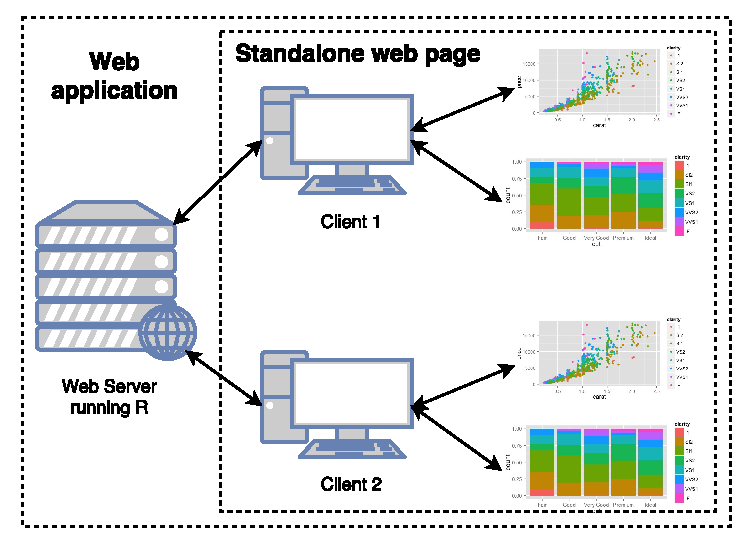
\includegraphics{images/server-client.pdf}
\caption{\label{fig:server-client}A basic visual depiction of linked views
in a standalone web page (A) versus a client-server model (B). In some
cases (A), linked views can be resolved within a web browser, which
generally leads to a better user experience. In other cases (B),
updating views may require calls to a web server running special
software.}
\end{figure}

At some rudimentary level, a programming interface like \textbf{shiny}
provides a way to design a graphical interface around programming
interface(s). This type of software not only enables people to share
their work with others in a user friendly fashion, but it can also make
their own work more efficient. In order to be efficient, the time
invested to create the GUI must be less than the amount of time it saves
by automating the programming task(s). And to empower this type of
efficiency, it helps tremendously to have programming interfaces that
work well together.

\subsection{Synergy among programming
interfaces}\label{synergy-among-programming-interfaces}

A typical data analysis workflow involves many different tasks, from
data acquistion, import, wrangling, visualization, modeling, and
reporting. Wickham and Grolemund (\protect\hyperlink{ref-r4ds}{2016})
points out the non-linear iteration between wrangling, visualization,
and modeling required to derive insights from data. Often times, each
stage requires one or more programming interface, and switching from one
interface to another can be frustrating since different interfaces often
have different philosophies. In some cases, the frustation involved from
transitioning from one interface to another is unavoidable, but in most
cases, working with a collection of interfaces that share the same
underlying principles helps alleviate friction. This is the motivation
behind the R package \textbf{tidyverse} which bundles numerous
interfaces for doing fundamental data analysis tasks based largely on
the tidy data framework (Wickham
\protect\hyperlink{ref-tidyverse}{2016}\protect\hyperlink{ref-tidyverse}{b});
(Wickham
\protect\hyperlink{ref-tidy-data}{2014}\protect\hyperlink{ref-tidy-data}{b}).

While tidy tools provide a nice cognitive framework for many common data
analysis tasks, sometimes it's necessary to work with messy (i.e.,
non-rectangular) data structures. In fact, Wickham and Grolemund
(\protect\hyperlink{ref-r4ds}{2016}) argues that 80\% of data analysis
tasks can be solved with tidy tools while the remaining 20\% requires
other tools. Probably the most common non-tidy data structure in R is
the nested list which is the most flexible and reliable way to represent
web-based data structures, such as JSON and XML, in R.

\section{Acquiring and wrangling web content in
R}\label{acquiring-and-wrangling-web-content-in-r}

\subsection{Interfaces for working with web
content}\label{interfaces-for-working-with-web-content}

R has a rich history of interfacing with web technologies for
accomplishing a variety of tasks such as requesting, manipulating, and
creating web content. As an important first step, extending ideas from
(Chambers \protect\hyperlink{ref-Chambers:1999}{1999}), Brian Ripley
implemented the connections interface for file-oriented input/output in
R (Ripley \protect\hyperlink{ref-Connections}{2001}). This interface
supports a variety of common transfer protocols (HTTP, HTTPS, FTP),
providing access to most files on the web that can be identified with a
Uniform Resource Locator (URL). Connection objects are actually external
pointers, meaning that, instead of immediately reading the file, they
just point to the file, and make no assumptions about the actual
contents of the file.

Many functions in the base R distribution for reading data (e.g.,
\texttt{scan}, \texttt{read.table}, \texttt{read.csv}, etc.) are built
on top of connections, and provide additional functionality for parsing
well-structured plain-text into basic R data structures (vector, list,
data frame, etc.). However, the base R distribution does not provide
functionality for parsing common file formats found on the web (e.g.,
HTML, XML, JSON). In addition, the standard R connection interface
provides no support for communicating with web servers beyond a simple
HTTP GET request (Lang \protect\hyperlink{ref-Lang:2006us}{2006}).

The \textbf{RCurl}, \textbf{XML}, and \textbf{RJSONIO} packages were
major contributions that drastically improved our ability to request,
manipulate, and create web content from R (Nolan and Temple Lang
\protect\hyperlink{ref-nolan-lang}{2014}). The \textbf{RCurl} package
provides a suite of high and low level bindings to the C library
libcurl, making it possible to transfer files over more network
protocols, communicate with web servers (e.g., submit forms, upload
files, etc.), process their responses, and handle other details such as
redirects and authentication (Temple Lang
\protect\hyperlink{ref-RCurl}{2014}\protect\hyperlink{ref-RCurl}{a}).
The \textbf{XML} package provides low-level bindings to the C library
libxml2, making it possible to download, parse, manipulate, and create
XML (and HTML) (Lang \protect\hyperlink{ref-XML}{2013}). To make this
possible, \textbf{XML} also provides some data structures for
representing XML in R. The \textbf{RJSONIO} package provides a mapping
between R objects and JavaScript Object Notation (JSON) (Temple Lang
\protect\hyperlink{ref-RJSONIO}{2014}\protect\hyperlink{ref-RJSONIO}{b}).
These packages were heavily used for years, but several newer interfaces
have made these tasks easier and more efficient.

The \textbf{curl}, \textbf{httr}, and \textbf{jsonlite} packages are
more modern R interfaces for requesting content on the web and
interacting with web servers. The \textbf{curl} package provides a much
simpler interface to libcurl that also supports streaming data (useful
for transferring large data), and generally has better performance than
\textbf{RCurl} (Ooms \protect\hyperlink{ref-curl}{2015}). The
\textbf{httr} package builds on \textbf{curl} and organizes it's
functionality around HTTP verbs (GET, POST, etc.) (Wickham
\protect\hyperlink{ref-httr}{2015}\protect\hyperlink{ref-httr}{a}).
Since most web application programming interfaces (APIs) organize their
functionality around these same verbs, it is often very easy to write R
bindings to web services with \textbf{httr}. The \textbf{httr} package
also builds on \textbf{jsonlite} since it provides consistent mappings
between R/JSON and most most modern web APIs accept and send messages in
JSON format (Ooms
\protect\hyperlink{ref-jsonlite}{2014}\protect\hyperlink{ref-jsonlite}{a}).
These packages have already had a profound impact on the investment
required to interface R with web services, which are useful for many
things beyond data acquisition. For example, it is now easy to install R
packages hosted on the web (\textbf{devtools}), perform cloud computing
(\textbf{analogsea}), and archive/share computational outputs
(\textbf{dvn}, \textbf{rfigshare}, \textbf{RAmazonS3},
\textbf{googlesheets}, \textbf{rdrop2}, etc.).

The \textbf{rvest} package builds on \textbf{httr} and makes it easy to
manipulate content in HTML/XML files (Wickham
\protect\hyperlink{ref-rvest}{2015}\protect\hyperlink{ref-rvest}{c}).
Using \textbf{rvest} in combination with
\href{http://selectorgadget.com/}{SelectorGadget}, it is often possible
to extract structured information (e.g., tables, lists, links, etc) from
HTML with almost no knowledge/familiarity with web technologies. The
\textbf{XML2R} package has a similar goal of providing an interface to
acquire and manipulate XML content into tabular R data structures
without any working knowledge of XML/XSLT/XPath (Sievert
\protect\hyperlink{ref-Sievert:2014a}{2014}\protect\hyperlink{ref-Sievert:2014a}{b}).
As a result, these interfaces reduce the start-up costs required for
analysts to acquire data from the web.

Packages such as \textbf{XML}, \textbf{XML2R}, and \textbf{rvest} can
download and parse the source of web pages, which is \emph{static}, but
extracting \emph{dynamic} web content requires additional tools. The R
package \textbf{rdom} fills this void and makes it easy to render and
access the Document Object Model (DOM) using the headless browsing
engine phantomjs (Sievert
\protect\hyperlink{ref-rdom}{2015}\protect\hyperlink{ref-rdom}{a}). The
R package \textbf{RSelenium} can also render dynamic web pages and
simulate user actions, but its broad scope and heavy software
requirements make it harder to use and less reliable compared to
\textbf{rdom} (Harrison \protect\hyperlink{ref-RSelenium}{2014}).
\textbf{rdom} is also designed to work seamlessly with \textbf{rvest},
so that one may use the \texttt{rdom()} function instead of
\texttt{read\_html()} to render, parse, and return the DOM as HTML
(instead of just the HTML page source).

Any combination of these R packages may be useful in acquiring data for
personal use and/or providing a higher-level interface to specific data
source(s) to increase their accessibility. The next section focuses on
such interfaces.

\subsection{Interfaces for acquiring data on the
web}\label{interfaces-for-acquiring-data-on-the-web}

The web provides access to the world's largest repository of publicly
available information and data. This provides a nice \emph{potential}
resource both teaching and practicing applied statistics, but to be
practical useful, it often requires a custom interface to make data more
accessible. If publishers follow best practices, a custom interface to
the data source usually is not needed, but this is rarely the case. Many
times structured data is embedded within larger unstructured documents,
making it difficult to incorporate into a data analysis workflow. This
is especially true of data used to inform downstream web applications,
typically in XML and/or JSON format. There are two main ways to make
such data more accessible: (1) package, document, and distribute the
data itself (2) provide functionality to acquire the data.

If the data source is fairly small, somewhat static, and freely
available with an open license, then we can directly provide data via R
packaging mechanism. In this case, it is best practice for package
authors include scripts used to acquire, transform, and clean the data.
This model is especially nice for both teaching and providing examples,
since users can easily access data by installing the R package. Wickham
(\protect\hyperlink{ref-rpkgs}{2015}\protect\hyperlink{ref-rpkgs}{b})
provides a nice section outlining the details of bundling data with R
packages.\footnote{This section is freely available online
  \url{http://r-pkgs.had.co.nz/data.html}.}

R packages that just provide functionality to acquire data can be more
desirable than bundling it for several reasons. In some cases, it helps
avoid legal issues with re-hosting copyrighted data. Furthermore, the
source code of R packages can always be inspected, so users can verify
the cleaning and transformations performed on the data to ensure its
integrity, and suggest changes if necessary. They are also versioned,
which makes the data acquisition, and thus any downstream analysis, more
reproducible and transparent. It is also possible to handle dynamic data
with such interfaces, meaning that new data can be acquired without any
change to the underlying source code. As explained in
\protect\hyperlink{taming-pitchfx-data-with-xml2r-and-pitchrx}{Taming
PITCHf/x Data with XML2R and pitchRx}, this is an important quality of
the \textbf{pitchRx} R package since new PITCHf/x data is made available
on a daily basis.

Perhaps the largest centralized effort in this domain is lead by
\href{https://ropensci.org}{rOpenSci}, a community of R developers that,
at the time of writing, maintains more than 50 packages providing access
to scientific data ranging from bird sightings, species occurrence, and
even text/metadata from academic publications. This provides a
tremendous service to researchers who want to spend their time building
models and deriving insights from data, rather than learning the
programming skills necessary to acquire and clean it.

It's becoming increasingly clear that ``meta'' packages that standardize
the interface to data acquisition/curation in a particular domain would
be tremendously useful. However, it is not clear how such interfaces
should be designed. The R package \textbf{etl} is one step in this
direction and aims to provide a standardized interface for \emph{any}
data access package that fits into an Extract-Transform-Load paradigm
(Baumer and Sievert \protect\hyperlink{ref-etl}{2016}). The package
provides generic \texttt{extract}-\texttt{transform}-\texttt{load}
functions, but requires package authors to write custom
\texttt{extract}-\texttt{transform} methods for the specific data
source. In theory, the default \texttt{load} method works for any
application; as well as other database management operations such as
\texttt{update} and \texttt{clean}.

\section{Interactive statistical web
graphics}\label{interactive-statistical-web-graphics}

\subsection{Why interactive graphics?}\label{why-interactive-graphics}

Unlike computer graphics which focuses on representing reality,
virtually; data visualization is about garnering abstract relationships
between multiple variables from visual representation. The
dimensionality of data, the number of variables can be anything, usually
more than 3D, which summons a need to get beyond 2D canvasses for
display. Technology enables this, allowing one to link multiple
low-dimensional displays in meaningful ways to reveal high-dimensional
structure. As demonstrated in Figure \ref{fig:touR} using the R package
\textbf{tourbrush} (Sievert
\protect\hyperlink{ref-tourbrush}{2015}\protect\hyperlink{ref-tourbrush}{b}),
interactive and dynamic statistical graphics allow us to go beyond the
constraints of low-dimensional displays to perceive high-dimensional
relationships in data.

\begin{figure}
\centering
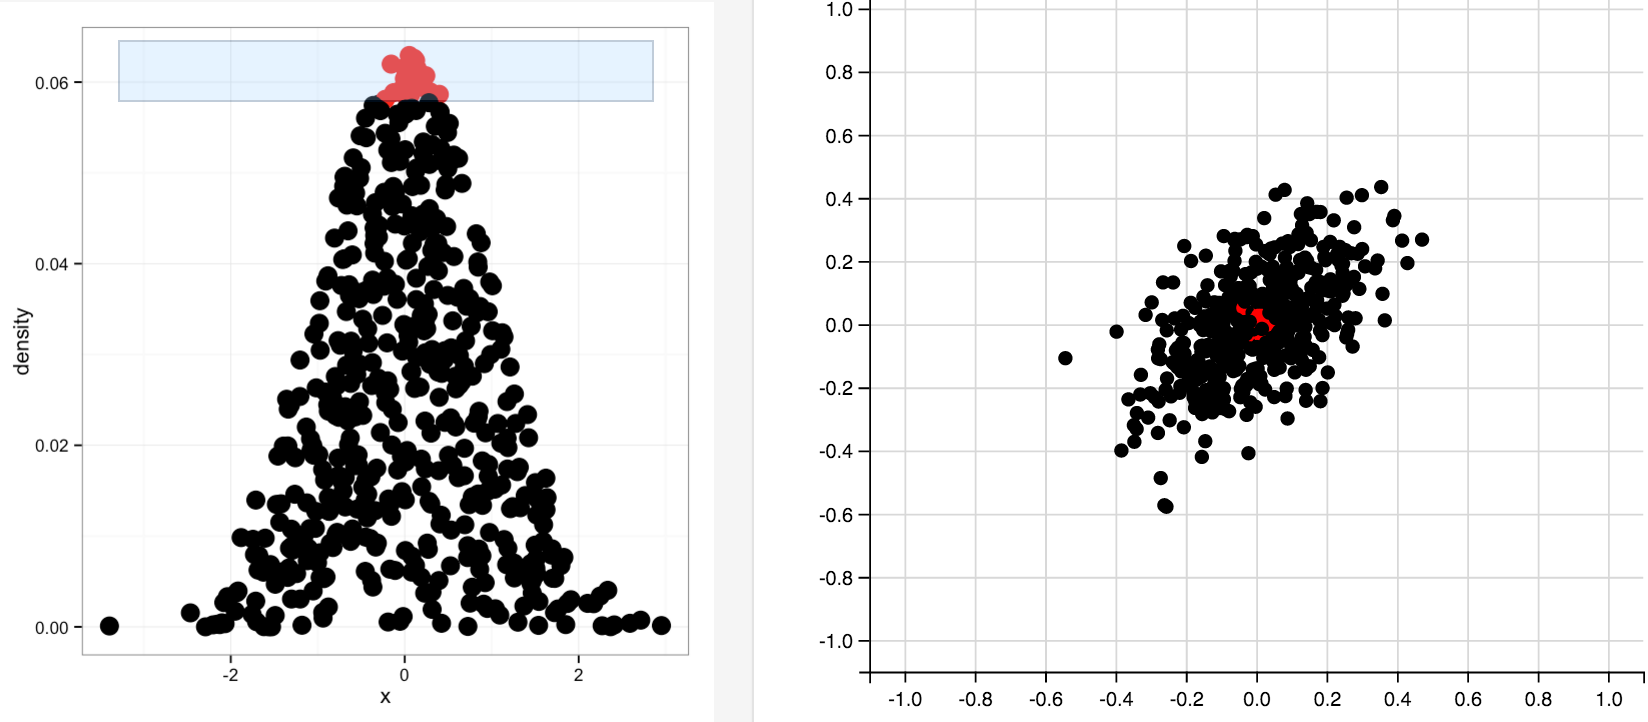
\includegraphics{images/tourbrush}
\caption{\label{fig:touR}A video demonstration of interactive and dynamic
techniques for visualizing high-dimensional relationships in data using
the R package \textbf{tourbrush}. You can view this movie online at
\url{https://vimeo.com/148050343}.}
\end{figure}

Interactive statistical graphics are a useful tool for descriptive
statistics, as well as for building better inferential models. Any
statistician is familiar with diagnosing a model by plotting data in the
model space (e.g., residual plot, qqplot). This works well for
determining if the assumptions of a model are adequate, but rarely
suggests that our model neglects important features in the data. To
combat this problem, Wickham, Cook, and Hofmann
(\protect\hyperlink{ref-Wickham:2015ur}{2015}\protect\hyperlink{ref-Wickham:2015ur}{a})
suggest to plot the model in the data space and use dynamic interactive
statistical graphics to do so. Interactive graphics have also proved to
be useful for exploratory model analysis, a situation where we have many
models to evaluate, compare, and critique (Unwin, Volinsky, and Winkler
\protect\hyperlink{ref-Unwin:2003uy}{2003}); (Urbanek
\protect\hyperlink{ref-Urbanek:2004}{2004}); (Ripley
\protect\hyperlink{ref-Ripley:2004}{2004}); (Unwin
\protect\hyperlink{ref-Unwin:2006}{2006}); (Wickham
\protect\hyperlink{ref-Wickham:2007wq}{2007}). With such power comes
responsibility that we can verify that visual discoveries are real, and
not due to random chance (Buja et al.
\protect\hyperlink{ref-Buja:2009hp}{2009}); (Majumder, Hofmann, and Cook
\protect\hyperlink{ref-Majumder:2013ie}{2013}).

Even within the statistical graphics community, the term
\emph{interactive} graphics can mean wildly different things to
different people (Swayne and Klinke
\protect\hyperlink{ref-swayne-klinke}{1999}). Some early statistical
literature on the topic uses interactive in the sense that a
command-line prompt allows users to create graphics on-the-fly (R. A.
Becker \protect\hyperlink{ref-S:1984}{1984}). That is, users enter
commands into a prompt, the prompts evaluates the command, and prints
the result (known as the read--eval--print loop (REPL)). Modifying a
command to generate another variation of a particular result (e.g., to
restyle a static plot) can be thought of as a type of interaction that
some might call \emph{indirect manipulation}.

Indirect manipulation can be achieved via a GUI or a programming (i.e.,
command-line) interface. Indirect manipulation from the command-line is
more flexible since we have complete control over the commands, but it
is also more cumbersome since we must translate our thoughts into code.
Indirect manipulation via a GUI is more restrictive, but it helps
reduces the gulf of execution (i.e., easier to generate desired output)
for end-users (Hutchins, Hollan, and Norman
\protect\hyperlink{ref-Hutchins:1985wu}{1985}). In this sense, a GUI can
be useful, even for experienced programmers, when the command-line
interface impedes the primary task of deriving insight from data.

In many cases, the gulf of execution can be further reduced through
direct manipulation. Roughly speaking, within the context of interactive
graphics, direct manipulation occurs whenever direct interaction with
plotting elements refocuses or reveals new information tied to the
event. Cook and Swayne (\protect\hyperlink{ref-ggobi:2007}{2007}) use
the terms dynamic graphics and direct manipulation to characterize
``plots that respond in real time to an analyst's queries and change
dynamically to re-focus, link to information from other sources, and
re-organize information.''

Although this thesis focuses on linked views, direct manipulation
encompasses many useful techniques that could be used, for example, to
re-focus a particular view. A simple example would be directly
manipulating the ordering of boxplots to enhance graphical analysis of
variance (ANOVA). By default, most plotting libraries sort categories
alphabetically, but this is usually not optimal for visual comparison of
groups. With a static plotting library such as \textbf{ggplot2}, we
could indirectly manipulate the default by going back to the
command-line, reordering the factor levels of the categorical variables,
and regenerate the plot (Wickham
\protect\hyperlink{ref-ggplot2}{2009}\protect\hyperlink{ref-ggplot2}{a}).
This is flexible and precise since we may order the levels by any
measure we wish (e.g., Median, Mean, IQR, etc.), but it would be much
quicker and easier if we had a GUI with a drop-down menu for most of the
reasonable sorting options. In a general purpose interactive graphics
system such as Mondrian, one can use direct manipulation to directly
click and drag on the categories to reorder them, making it quick and
easy to compare any two groups of interest (Theus and Urbanek
\protect\hyperlink{ref-mondrianbook}{2008}).

The ASA Section on Statistical Computing and Graphics maintains a video
library which captures many useful interactive statistical graphics
techniques. Several videos show how XGobi (predecessor to GGobi), a
dynamic interactive statistical graphics system, can be used to reveal
high-dimensional relationships and structures that cannot be easily
identified using numerical methods alone (Swayne, Cook, and Buja
\protect\hyperlink{ref-xgobi}{1998}).\footnote{For example,
  \url{http://stat-graphics.org/movies/xgobi.html} and
  \url{http://stat-graphics.org/movies/grand-tour.html}} Another notable
video shows how the interactive graphics system Mondrian can be used to
quickly find interesting patterns in high-dimensional data using
exploratory data analysis (EDA) techniques (Theus and Urbanek
\protect\hyperlink{ref-mondrianbook}{2008}).\footnote{\url{http://stat-graphics.org/movies/tour-de-france.html}}
The most recent video shows how dynamic interactive techniques can help
interpret a topic model (a statistical mixture model applied to text
data) using the R package \textbf{LDAvis} (Sievert and Shirley
\protect\hyperlink{ref-Sievert:2014b}{2014}), which is the first
web-based visualization in the library, and is discussed at depth in
\protect\hyperlink{ldavis-a-method-for-visualizing-and-interpreting-topics}{LDAvis:
A method for visualizing and interpreting topics}.

In order to be practically useful, interactive statistical graphics must
be fast, flexible, accessible, portable, and reproducible. In general,
over the last 20-30 years interactive graphics systems were fast and
flexible, but were generally not easily accessible, portable, or
reproducible. The web browser provides a convenient platform to combat
these problems. For example, any visualization created with
\textbf{LDAvis} can be shared through a Uniform Resource Locator (URL),
meaning that anyone with a web browser and an internet connection can
view and interact with a visualization. Furthermore, we can link anyone
to any possible state of the visualization by encoding selections with a
URL fragment identifier. This makes it possible to link readers to an
interesting state of a visualization from an external document, while
still allowing them to independently explore the same visualization and
assess conclusions drawn from it.\footnote{A good example is
  \url{http://cpsievert.github.io/LDAvis/reviews/reviews.html}}

\subsection{Web graphics}\label{web-graphics}

Thanks to the constant evolution and eventual adoption of HTML5 as a web
standard, the modern web browser now provides a viable platform for
building an interactive statistical graphics systems. HTML5 refers to a
collection of technologies, each designed to perform a certain task,
that work together in order to present content in a web browser. The
Document Object Model (DOM) is a convention for managing all of these
technologies to enable \emph{dynamic} and \emph{interactive} web pages.
Among these technologies, there are several that are especially relevant
for interactive web graphics:

\begin{enumerate}
\def\labelenumi{\arabic{enumi}.}
\tightlist
\item
  HTML: A markup language for structuring and presenting web content.
\item
  SVG: A markup language for drawing scalable vector graphics.
\item
  CSS: A language for specifying styling of web content.
\item
  JavaScript: A language for manipulating web content.
\end{enumerate}

Juggling all of these technologies just to create a simple statistical
plot is a tall order. Thankfully, HTML5 technologies are publicly
available, and benefit from thriving community of open source developers
and volunteers. In the context of web-based visualization, the most
influential contribution is Data Driven Documents (D3), a JavaScript
library which provides high-level semantics for binding data to web
content (e.g., SVG elements) and orchestrating scene updates/transitions
(Heer \protect\hyperlink{ref-Bostock:2011}{2011}). D3 is wildly
successful because is builds upon web standards, without abstracting
them away, which fosters customization and interoperability. However,
compared to a statistical graphics environments like R, creating basic
charts is complicated, and a large amount of code must be customized for
each visualization. As a result, web graphics are widely used for
presentation graphics (visualization type is known), but are not (yet!)
practically useful for exploratory graphics (visualization type is not
known).

There are a number of projects attempting to make interactive web
graphics more practically useful for ad-hoc data analysis tasks. For
statisticians and other people working with data, this means the
interface should look and feel like other graphing interfaces in R where
many of the rendering details are abstracted away allowing the user to
focus on data analysis. The next section discusses some approaches that
provide a direct translation of R graphics to a web-based format --
requiring essentially no additional effort by existing R users to take
advantage of them. The section afterwards discusses other approaches
which design a brand-new R interface for creating web graphics.

\subsection{Translating R graphics to the
web}\label{translating-r-graphics-to-the-web}

There are a few ways to translate R graphics to a web format, such as
SVG. R has built-in support for a SVG graphics device, made available
through the \texttt{svg()} function, but it can be quite slow, which
inspired the new \textbf{svglite} package (Wickham et al.
\protect\hyperlink{ref-svglite}{2016}). The \texttt{grid.export()}
function from the \textbf{gridSVG} package also provides an SVG device,
designed specifically for \textbf{grid} graphics (e.g.,
\textbf{ggplot2}, \textbf{lattice}, etc.).\footnote{The
  \textbf{gridGraphics} package makes it possible to draw \textbf{base}
  graphics as \textbf{grid} graphics -- meaning that \textbf{gridSVG}
  can (indirectly) convert any R graphic.} It adds the ability to retain
structured information about grid objects in the SVG output, making it
possible to layer on interactive functionality (Potter and Murrell
\protect\hyperlink{ref-gridSVGreport}{2012}). The \textbf{rvg} package
is a similar project, but implements its own set of graphics devices to
support SVG output as well as proprietary XML-based formats (e.g., Word,
Powerpoint, XLSX) (Gohel
\protect\hyperlink{ref-rvg}{2016}\protect\hyperlink{ref-rvg}{b}).

A number of projects attempt to layer interactivity on top of a SVG
output generated from R code an SVG graphics device. The
\textbf{SVGAnnotation} package was the first attempt at post-processing
SVG files (created via \texttt{svg()}) to add some basic interactivity
including: tooltips, animation, and even linked brushing via mouse hover
(Nolan and Temple Lang
\protect\hyperlink{ref-SVGAnnotation}{2012}).\footnote{Unfortunately,
  this package now serves as a proof of concept as most examples are now
  broken, and no one has contributed to the project in 3 years.} The
\textbf{ggiraph} package is a more modern approach using a similar idea.
It uses the \textbf{rvg} package to generate SVG output via a custom
graphics device; but focuses specifically on extending
\textbf{ggplot2}'s interface, and currently has no semantics for linking
plots (Gohel
\protect\hyperlink{ref-ggiraph}{2016}\protect\hyperlink{ref-ggiraph}{a}).
There are also a number of notable projects that layer interactivity on
top of SVG output provided by \textbf{gridSVG}'s graphics device,
including \textbf{vdmR} which enables (very limited support for) linked
brushing between \textbf{ggplot2} graphics and \textbf{svgPanZoom} which
adds zooming and panning (Fujino \protect\hyperlink{ref-vdmR}{2015});
(Riutta et. al. and Russell \protect\hyperlink{ref-svgPanZoom}{2015}).
Translating R graphics at this level is a fundamentally limited
approach, however, because it loses information about the raw data and
its mapping to visual space.

The \textbf{animint} and \textbf{plotly} packages take a different
approach in translating \textbf{ggplot2} graphics to a web format
(Hocking, VanderPlas, and Sievert
\protect\hyperlink{ref-animint}{2015}); (Sievert et al.
\protect\hyperlink{ref-plotly}{2016}). Instead of translating directly
to SVG via \textbf{gridSVG}, they extract relevant information from the
internal representation of a \textbf{ggplot2} graphic\footnote{For a
  visual display of the internal representation used to render a
  \textbf{ggplot2} graph, see my \textbf{shiny} app here
  \url{https://gallery.shinyapps.io/ggtree}.}, store it in JavaScript
Object Notation (JSON), and pass the JSON as an input to a JavaScript
function, which then produces a web based visualization. This design
pattern is popular among modern web-based graphing libraries, since it
separates out \emph{what} information is contained in the graphic from
\emph{how} to actually draw it. This has a number of advantages; for
example, \textbf{plotly} graphics can be rendered in SVG, or using WebGL
(based on HTML5 canvas, not SVG) which allows the browser to render many
more graphical marks by leveraging the GPU. It also has the advantage of
more extensible from R since novel features can be enabled by adding to
and/or modifying the underlying data structure (instead of writing
ad-hoc JavaScript code to modify the DOM).

Translating existing R graphics to a web-based format is useful for
quickly enabling some basic interactivity, but an extension of the
underlying graphics interface may be required to enable more advanced
features (e.g.~linked views). For example, in both \textbf{animint} and
\textbf{plotly}, we automatically provide tooltips (which reveal more
information about each graphical mark on mouse hover) and clickable
legends that show/hide graphical marks corresponding to the legend
entry. The \textbf{animint} package extends \textbf{ggplot2}'s grammar
of graphics implementation to enable animations and linked views with
relatively small amount of effort required by those familiar with
\textbf{ggplot2}. This extension is discussed at length in the chapter
\protect\hyperlink{animint}{Extending ggplot2's grammar of graphics
implementation for linked and dynamic graphics on the web}. The
\textbf{plotly} package supersedes \textbf{animint} to support a larger
taxonomy of interaction types (e.g., hover, click, click+drag),
interaction modes (e.g., dynamically controllable persistent brush),
chart types (e.g., 3D surfaces), and even provides a consistent
interface for enabling animation/linked-views across graphs created via
\textbf{ggplot2} or its own custom (non-ggplot2) interface. These
features are discussed in
\href{https://cpsievert.github.io/plotly_book/}{plotly for R}.

\hypertarget{interfacing-with-interactive-web-graphics}{\subsection{Interfacing
with interactive web
graphics}\label{interfacing-with-interactive-web-graphics}}

Although it is more onerous for users to learn a new interface, there
are a number of advantages to designing a new R interface (that is
independent of any translation) to a web graphics system. For one, the
translation may require assumptions about internal workings of another
system, making it vulnerable to changes in that system. Moreover, a new
interface may be designed to take advantage of \emph{all} the features
available in the web graphics system. In some cases, the custom
interface can even be used to provide an elegant way to extend the
functionality of a translation mechanism, as described in
\protect\hyperlink{extending-ggplotlyux28ux29}{Extending
\texttt{ggplotly()}}.

An early attempt to design an R interface for general purpose
interactive web graphics was the R package \textbf{rCharts} whose R
interface is heavily inspired by \textbf{lattice} (Vaidyanathan
\protect\hyperlink{ref-rCharts}{2013}); (Sarkar
\protect\hyperlink{ref-lattice}{2008}). The most innovative part of
\textbf{rCharts} was its ability to interface with many different
JavaScript graphing libraries using a single R interface. As the number
of JavaScript graphing libraries began to explode, it became obvious
this was not a sustainable model, as the R package must bundle each
JavaScript library that it supports. However, a lot of the
infrastructure, such as providing the glue to render plots in various
contexts (e.g., the R console, shiny apps, and \textbf{rmarkdown}
documents), have evolved into the R package \textbf{htmlwidgets}
(Vaidyanathan et al. \protect\hyperlink{ref-htmlwidgets}{2015}). Having
built similar bridges for \textbf{animint} and \textbf{LDAvis}, I
personally know and appreciate the amount of time and effort this
package saves other package authors.

The \textbf{htmlwidgets} framework is not constrained to just graphics,
it simply provides a set of conventions for authoring web content from
R. Numerous JavaScript data visualization libraries are now made
available using this framework, and most are designed for particular use
cases, such as \textbf{leaflet} for geo-spatial mapping,
\textbf{dygraphs} for time-series, and \textbf{networkD3} for networks
(Cheng and Xie \protect\hyperlink{ref-leaflet}{2015}); (Vanderkam and
Allaire \protect\hyperlink{ref-dygraphs}{2015}); (Gandrud, Allaire, and
Russell \protect\hyperlink{ref-networkD3}{2015})\footnote{For more
  examples and information, see \url{http://www.htmlwidgets.org/} and
  \url{http://hafen.github.io/htmlwidgetsgallery/}}. There are also HTML
widgets that provide an interface to more general purpose visualization
JavaScript libraries such as \textbf{plotly} and \textbf{rbokeh}
(Sievert et al. \protect\hyperlink{ref-plotly}{2016}); (Hafen and team
\protect\hyperlink{ref-rbokeh}{2015}).

Many \textbf{htmlwidgets} provide at least some native support for
direct manipulation such as identifying (i.e., mousing over points to
reveal labels), focusing (i.e., pan and zoom), and sometimes linking
multiple views (i.e., animation, brushing over points to highlight
points in another view, etc). In some cases, this interactivity is
handled entirely by the underlying JavaScript library, but
\textbf{htmlwidgets} authors may also provide an R interface to custom
JavaScript based logic to extend the interface's functionality. The R
package \textbf{plotly} uses this approach to enable features not found
in plotly.js' JSON specification, such as linked views. To understand
how it works, it helps to know about Model-View-Controller (MVC)
paradigm, and the different ways to approach MVC in a web-based
environment.

\subsection{Multiple MVC paradigms}\label{multiple-mvc-paradigms}

The Model-View-Controller (MVC) paradigm is a popular programming
technique for designing graphical user interfaces with a minimal amount
of dependencies which helps increase responsiveness. Responsiveness is
absolutely crucial for interactive graphics since it greatly impacts our
ability to make observations, draw generalizations, and generate
hypotheses (Z. L. A. J. Heer
\protect\hyperlink{ref-2014-latency}{2014}). In a MVC paradigm, the
model contains all the data and logic necessary to generate view(s). The
controller can be thought of as a component on top of a view that
listens for certain events, and feeds those events to the model so that
the model can update view(s) accordingly. As Figure \ref{fig:mvc} shows,
modern R interfaces to interactive web graphics should have multiple
model(s) that reside in different places (depending the event type).

\begin{figure}
\centering
\includegraphics{images/mvc}
\caption{\label{fig:mvc}Four different MVC paradigms. In all the scenarios,
the graph acts as the controller, but the model (i.e., the data and
logic which updates the view) exists in different places. In Scenario A,
a mouse hover event manipulates the model within the underlying
JavaScript library. In Scenario B, a window resizing manipulates the
model within the HTMLwidget.resize() method, defined by the widget
author. In Scenario C, a mouse hover event manipulates the model within
the underlying JavaScript library \emph{and} a model defined by both the
user (in R) and the widget author (in JavaScript). In Scenario D,
removing outliers from the raw data may require R code to be executed.}
\end{figure}

For relatively simple interactions, like identification (scenario A/C)
and resizing (scenario B) in Figure \ref{fig:mvc}, the model should
reside within the web browser. Many JavaScript libraries have a native
MVC paradigm for manipulating a single graph, like drawing tooltips on
mouse hover (scenario A), but there may be other useful manipulation
events that the paradigm doesn't support. This could be result of the
fact that the JavaScript library simply does not know about the R
interface. For example, resizing should work consistently across various
contexts (whether viewing in RStudio, \textbf{shiny} apps,
\textbf{rmarkdown} documents, etc). Thankfully the \textbf{htmlwidgets}
package provides a JavaScript library that triggers a \texttt{resize()}
event whenever the window size changes within any of these contexts --
allowing the widget author to focus on the resizing model rather
defining all the possible controllers.

For more complicated interactions, the model may have to be defined in R
by the user, even when manipulating a single graph. Even when the model
is defined in R, that does not necessarily imply the controller requires
a hook back to re-execute R code. For example, scenario C in Figure
\ref{fig:mvc} details a situation where the R user has specified that
lines should be highlighted upon hover from the R interface, which is
not natively supported by the underlying JavaScript graphing library,
but can be implemented by the widget author by providing a framework
which translates a model from R to JSON (+ custom JavaScript). In any
case, the widget author should take special care not to trigger a full
redraw of the plot, and do the minimal amount of work necessary to
update the view. For example, in scenario C, the lines are highlighted
by simply reducing the opacity of the non-selected lines. In fact, all
of the examples in the section
\protect\hyperlink{linking-views-without-shiny}{linking views without
shiny} follow this paradigm (scenario C).

A callback to re-execute R code is only necessary if the model requires
information that is not already contained in the JSON object and
JavaScript logic. So, for scenario D in Figure \ref{fig:mvc}, it is
theoretically possible to precompute linear models for every possible
view and let the browser handle the MVC paradigm. However, this approach
does not scale well, so it is often more practical to have the
controller trigger callbacks to R. To provide access to a controller in
\textbf{shiny}, htmlwidget authors need to leverage the JavaScript
function \texttt{Shiny.onInputChange()} to inform the \textbf{shiny}
server (i.e., the model) about a certain event. Here is a hypothetical
and over-simplified example where \texttt{view} is an object
representing a particular graph/view which has an \texttt{on()} method
that triggers the execution of a function whenever a
\texttt{"mouse\_hover"} on this view happens.

\begin{Shaded}
\begin{Highlighting}[]
\VariableTok{view}\NormalTok{.}\AttributeTok{on}\NormalTok{(}\StringTok{"mouse_hover"}\OperatorTok{,} \KeywordTok{function}\NormalTok{(d) }\OperatorTok{\{}
  \VariableTok{Shiny}\NormalTok{.}\AttributeTok{onInputChange}\NormalTok{(}\StringTok{"mouse_hover"}\OperatorTok{,} \NormalTok{d)}\OperatorTok{;}
\OperatorTok{\}}\NormalTok{)}
\end{Highlighting}
\end{Shaded}

Users may then subscribe to the event in a \textbf{shiny} app by
accessing the event in the server logic (a R function which allows one
to access \texttt{input} values, manipulate them, and generate output).
Assuming the data attached the event (\texttt{d}) simply contains the
\texttt{id} property defined in \texttt{scatterplot()}, this is one way
you could modify the color of a point by hovering on it.

\begin{Shaded}
\begin{Highlighting}[]
\NormalTok{function(input, output) \{}
  \NormalTok{x <-}\StringTok{ }\DecValTok{1}\NormalTok{:}\DecValTok{10}
  \NormalTok{y <-}\StringTok{ }\KeywordTok{rnorm}\NormalTok{(}\DecValTok{10}\NormalTok{)}
  \NormalTok{output$view <-}\StringTok{ }\KeywordTok{renderWidget}\NormalTok{(\{}
    \NormalTok{isSelected <-}\StringTok{ }\NormalTok{x ==}\StringTok{ }\NormalTok{input$mouse_hover}
    \KeywordTok{scatterplot}\NormalTok{(x, y, }\DataTypeTok{id =} \NormalTok{x, }\DataTypeTok{color =} \NormalTok{isSelected)}
  \NormalTok{\})}
\NormalTok{\}}
\end{Highlighting}
\end{Shaded}

As previously mentioned, this example is over-simplified for the purpose
of demonstrating the basic approach to subscribing a controller in
\textbf{shiny}. A proper implementation should also scope input values
by view, so users can distinguish events from different views. The
section on \protect\hyperlink{targeting-views}{Targeting views} gives an
example of why scoping is important.

Recently, \textbf{shiny} used this approach to allows users to add
controllers on top of static R graphics\footnote{This website shows what
  information is sent from the client to the server when users interact
  with plot(s) via mouse event(s) --
  \url{http://shiny.rstudio.com/gallery/plot-interaction-basic.html}},
effectively allowing developers to coordinate views in a web app, with
no JavaScript involved. Although this is a useful tool, it is
fundamentally limited, since updates to a static image will always
require a full redraw. More specifically, within the MVC paradigm
context, static images require the entire model (the logic for updating
the view) to reside on the server and very rarely can images be sent to
the client fast enough to appear instantaneous.

The touring video in Figure \ref{fig:touR} helps point out why these
limitations matter. Notice that when a brush event occurs on the left
hand panel (a static graphic), the entire view must be flushed and
repopulated to provide a visual clue for the selection, resulting in a
``glitch'' effect. If that view was web-based, it would be possible to
provide a visual clue without the glitch effect. This glitching effect
would seriously limit the usefulness of the visualization if the right
hand panel of Figure \ref{fig:touR} also had to be flushed for every
animation frame. Fortunately, that view is web-based, and can smoothly
transition from one frame to the next when it receives new data from the
R server, thanks to its hybrid MVC paradigm.

\subsection{Hybrid MVC for one
interface}\label{hybrid-mvc-for-one-interface}

Without a doubt, the MVC paradigm depicted in scenario D of Figure
\ref{fig:mvc} provides a powerful foundation for interactive statistical
graphics. In fact, if interactive web graphics are to replicate and
extend classical approaches to the subject, they should follow this
paradigm to leverage the statistical facilities that R provides, but
\emph{only} when it is necessary, since requiring the browser to
communicate with an external R process is costly on multiple levels.
That being said, assuming the additional infrastructure is required, it
can be very useful to share semantics between R and JSON/JavaScript so
that the browser can receive dynamically changing data from an R server
and be smart and efficient when updating the view.

A great example of a hybrid MVC can be found in the R package
\textbf{ggvis}, a reworking of ggplot2's grammar of graphics to
incorporate interactivity (Chang and Wickham
\protect\hyperlink{ref-ggvis}{2015}). In \textbf{ggvis}, graphs are
created with either an ordinary data frame or a special \emph{reactive}
data frame (i.e., a reactive expression in \textbf{shiny} that outputs a
data frame). The JavaScript model is aware of these special reactive
data frames, and there mapping to visual space, so that when the
JavaScript model receives new data, it can avoid a full redraw and only
modify the visual properties for values that have changed. This not only
enables updates from one view to the next to appear instaneous to the
user, it also opens up the possibility of smoothly transitioning
specific objects from one view to the next (i.e., interpolating between
views). Smooth transitions help facilitate object constancy (i.e.,
tracking an object from one view to the next) which can improve
graphical perception (Heer and Robertson
\protect\hyperlink{ref-animated-transitions}{2007}).

Another nice example of a hybrid MVC can be found in the R package
\textbf{leaflet}, an interface to the popular JavaScript library for
interactive maps. Although its hybrid MVC requires the map to be
embedded within a \textbf{shiny} app, it allows one to modify graphical
markings laid on top of a map without redrawing the map itself.

A hybrid MVC does not have to rely on \textbf{shiny}, and in fact, it
can be used link multiple views without requiring a full redraw or R
code to be re-executed. Furthermore, it can be implemented in such a way
that is arguably easier to express from R compared to a full-blown
\textbf{shiny} app. Figure \ref{fig:scenarios} gives a high-level
overview of how this works in the \textbf{plotly} package. Scenario B
shows a situation where a brush event manipulates a model defined in a
\textbf{shiny} app (via the \texttt{event\_data()} function) which
requires a full redraw. Scenario A shows a situation where a brush event
directly manipulates a linked view via a \textbf{plotly}'s hybrid MVC
model; and in this case, the JavaScript function
\texttt{Plotly.restyle()} is used to simply modify the color the
selected points in both views and reduce the opacity of non-selected
points.

\begin{figure}
\centering
\includegraphics{images/scenarios}
\caption{\label{fig:scenarios}Linking views in plotly with shiny (scenario
B) versus without shiny (scenario A).}
\end{figure}

\subsection{MVC for multiple
interfaces}\label{mvc-for-multiple-interfaces}

As mentioned in
\protect\hyperlink{interfacing-with-interactive-web-graphics}{Interfacing
with interactive web graphics}, there is now a diverse collection of R
packages that interface with JavaScript graphing libraries. Since these
interfaces generate web-based output, we may start to envision a hybrid
MVC paradigm for linking views between different interfaces
\emph{without} a client-server infrastructure like \textbf{shiny}. For
convenience, I will refer to this paradigm as a \emph{centralized}
pipeline, which is depicted on the right-hand side of Figure
\ref{fig:central-pipeline}. Since centralized pipelines cannot
dynamically re-execute R code, they are somewhat limited in their
ability to dynamically transform raw data compared to data pipelines
discussed by Andreas Buja and McDonald
(\protect\hyperlink{ref-viewing-pipeline}{1988}) and Lawrence
(\protect\hyperlink{ref-ggobi-pipeline-design}{2002}). Figure
\ref{fig:central-pipeline} attempts to show this limitation in direct
comparison to the GGobi pipeline, but also highlight the benefit of
enabling linked views between arbitrary systems (and easily sharing
them). As it turns out, a centralized pipeline is sufficient for
creating a fairly large class of useful interactive graphics, and thanks
to tools like \textbf{shiny}, users may still opt into a server-client
infrastructure, if need be.

\begin{figure}
\centering
\includegraphics{images/ggobi-pipeline}
\caption{\label{fig:central-pipeline}The GGobi pipeline, as described by
Lawrence (\protect\hyperlink{ref-ggobi-pipeline-design}{2002}), in
comparison to a centralized pipeline. The GGobi pipeline is shown in
peach color while the centralized pipeline is in both yellow and blue to
point out multiple interfaces can be linked in a centralized pipeline.}
\end{figure}

In a centralized pipeline, the first thing that is needed is a way to
declare a link between the views from R. There are multiple ways to
approach linking, but Figure \ref{fig:crosstalk} defines a link between
views using a primary key relationship (in the data sets used to create
each view), analogous to an approach first described by Buja et al.
(\protect\hyperlink{ref-Buja:1991vh}{1991}). A primary key relationship
is more flexible than a unique key in the sense that the column used to
define the key can have multiple rows with the same value. This
flexibility allows m-to-n linking (e.g.~select m rows in one data set
and n in another) to happen. For example, in Figure \ref{fig:crosstalk},
a brush selects three cities, which is tied to 30 about rows in the data
behind the parallel coordinate plot, but only 3 rows in the data behind
the map. Assuming this primary key is translated to JSON, the client has
\emph{access to} enough information to update the views -- but the model
(i.e., the logic for updating view(s)) has to be implemented separately
by each interface (in JavaScript).

\begin{figure}
\centering
\includegraphics{images/crosstalk}
\caption{\label{fig:crosstalk}The MVC design for linking multiple
htmlwidgets with crosstalk}
\end{figure}

To enable linked views between multiple R interfaces, as in Figure
\ref{fig:crosstalk}, it helps to have standards for both defining a
primary key from R (done by the user) and to set/access primary key
selections in JavaScript (done by the developer). The new R package
\textbf{crosstalk} proposes a \texttt{SharedData} class in R that allows
one to add this primary key attribute to data frames (Cheng
\protect\hyperlink{ref-crosstalk}{2015}\protect\hyperlink{ref-crosstalk}{a}).
It also provides a JavaScript library for setting, storing, and
accessing selection values in the browser, but leaves the actual logic
for updating views to widget authors. In a sense, this project is
similar to the work of North and Shneiderman
(\protect\hyperlink{ref-North:1999vi}{1999}), which provided standards
for ``snapping together'' arbitrary views that are aware of a relational
database schema, but \textbf{crosstalk} does so in a web-based
environment, rather than requiring a machine running Windows.

The first HTML widget to leverage \textbf{crosstalk} was Cheng
(\protect\hyperlink{ref-d3scatter}{2015}\protect\hyperlink{ref-d3scatter}{b}),
but is currently limited to linked scatterplot brushing.\footnote{See,
  for example, \url{http://rpubs.com/jcheng/crosstalk-demo}} Currently,
there are a couple other R packages with \textbf{crosstalk} support,
including \textbf{leaflet} and \textbf{DT} (Xie
\protect\hyperlink{ref-DT}{2015}), but \textbf{plotly} is the only
package with some support for the data pipeline, different selection
modes (transient vs persistent selection), and different interaction
types (e.g., mouse hover, click, and multiple types of click+drag
selections). The pedestrians case study in
\protect\hyperlink{plotly-for-R}{plotly for R} provides an example of
linking views between \textbf{leaflet} and \textbf{plotly} via
\textbf{crosstalk} to quickly pose queries about high-dimensional data.
The section \protect\hyperlink{linking-views-without-shiny}{linking
views without shiny} provides many examples designed to teach the reader
how to use \textbf{plotly} and \textbf{crosstalk} to link views in
numerous scenarios.

\chapter{Scope}

Explain your contributions to each project

\url{https://github.com/ropensci/plotly/graphs/contributors}

\chapter{Taming PITCHf/x Data with XML2R and pitchRx}

This chapter is a paper published in \emph{The R Journal} (Sievert
\protect\hyperlink{ref-Sievert:2014a}{2014}\protect\hyperlink{ref-Sievert:2014a}{b}).
I am the sole author of the paper which is avaliable online here
\url{https://journal.r-project.org/archive/2014-1/sievert.pdf}

The formatting of paper has been modified to make for consistent
typesetting across the thesis.

\specialchapt{ABSTRACT}

\textbf{XML2R} is a framework that reduces the effort required to
transform XML content into tables in a way that preserves parent to
child relationships. \textbf{pitchRx} applies \textbf{XML2R}'s grammar
for XML manipulation to Major League Baseball Advanced Media (MLBAM)'s
Gameday data. With \textbf{pitchRx}, one can easily obtain and store
Gameday data in a remote database. The Gameday website hosts a wealth of
XML data, but perhaps most interesting is PITCHf/x. Among other things,
PITCHf/x data can be used to recreate a baseball's flight path from a
pitcher's hand to home plate. With \textbf{pitchRx}, one can easily
create animations and interactive 3D scatterplots of the baseball's
flight path. PITCHf/x data is also commonly used to generate a static
plot of baseball locations at the moment they cross home plate. These
plots, sometimes called \textit{strike-zone plots}, can also refer to a
plot of event probabilities over the same region. \textbf{pitchRx}
provides an easy and robust way to generate strike-zone plots using the
\textbf{ggplot2} package.

\section{Introduction}\label{introduction}

\subsection{What is PITCHf/x?}\label{what-is-pitchfx}

PITCHf/x is a general term for a system that generates a series of 3D
measurements of a baseball's path from a pitcher's hand to home plate
(Alt and White \protect\hyperlink{ref-patent}{2008}).
\footnote{A \textit{pitcher} throws a ball to the opposing \textit{batter}, who
stands besides home plate and tries to hit the ball into the field
of play.
} In an attempt to estimate the location of the ball at any time point,
a quadratic regression model with nine parameters (defined by the
equations of motion for constant linear acceleration) is fit to each
pitch. Studies with access to the actual measurements suggest that this
model is quite reasonable -- especially for non-knuckleball pitches
(Nathan \protect\hyperlink{ref-trajecoryAnalysis}{2008}). That is, the
fitted path often provides a reasonable estimate (within a couple of
inches) of the actual locations. Unfortunately, only the parameter
estimates are made available to the public. The website that provides
these estimates is maintained by MLBAM and hosts a wealth of other
baseball related data used to inform MLB's Gameday webcast service in
near real time.

\subsection{Why is PITCHf/x important?}\label{why-is-pitchfx-important}

On the business side of baseball, using statistical analysis to scout
and evaluate players has become mainstream. When PITCHf/x was first
introduced, DiMeo (\protect\hyperlink{ref-slate}{2007}) proclaimed it
as,

\begin{quote} ``The new technology that will change statistical analysis [of baseball] forever.'' \end{quote}

PITCHf/x has yet to fully deliver this claim, partially due to the
difficulty in accessing and deriving insight from the large amount of
complex information. By providing better tools to collect and visualize
this data, \textbf{pitchRx} makes PITCHf/x analysis more accessible to
the general public.

\subsection{PITCHf/x applications}\label{pitchfx-applications}

PITCHf/x data is and can be used for many different projects. It can
also complement other baseball data sources, which poses an interesting
database management problem. Statistical analysis of PITCHf/x data and
baseball in general has become so popular that it has helped expose
statistical ideas and practice to the general public. If you have
witnessed television broadcasts of MLB games, you know one obvious
application of PITCHf/x is locating pitches in the strike-zone as well
as recreating flight trajectories, tracking pitch speed, etc. Some
on-going statistical research related to PITCHf/x includes: classifying
pitch types, predicting pitch sequences, and clustering pitchers with
similar tendencies (Pane et al. \protect\hyperlink{ref-curve}{2013}).

\subsection[Contributions of pitchRx and XML2R]{Contributions of \textbf{pitchRx} and \textbf{XML2R}}

The \textbf{pitchRx} package has two main focuses (Sievert
\protect\hyperlink{ref-pitchRx}{2014}\protect\hyperlink{ref-pitchRx}{a}).
The first focus is to provide easy access to Gameday data. Not only is
\textbf{pitchRx} helpful for collecting this data in bulk, but it has
served as a helpful teaching and research aide
(\url{http://baseballwithr.wordpress.com/} is one such example). Methods
for collecting Gameday data existed prior to \textbf{pitchRx}; however,
these methods are not easily extensible and require juggling
technologies that may not be familiar or accessible (Fast
\protect\hyperlink{ref-database}{2007}). Moreover, these working
environments are less desirable than R for data analysis and
visualization. Since \textbf{pitchRx} is built upon \textbf{XML2R}'s
united framework, it can be easily modified and/or extended (Sievert
\protect\hyperlink{ref-XML2R}{2014}\protect\hyperlink{ref-XML2R}{c}).
For this same reason, \textbf{pitchRx} serves as a model for building
customized XML data collection tools with \textbf{XML2R}.

The other main focus of \textbf{pitchRx} is to simplify the process
creating popular PITCHf/x graphics. Strike-zone plots and animations
made via \textbf{pitchRx} utilize the extensible \textbf{ggplot2}
framework as well as various customized options (Wickham
\protect\hyperlink{ref-ggplot2}{2009}\protect\hyperlink{ref-ggplot2}{a}).
\textbf{ggplot2} is a convenient framework for generating strike-zone
plots primarily because of its facet schema which allows one to make
visual comparisons across any combination of discrete variable(s).
Interactive 3D scatterplots are based on the \textbf{rgl} package and
useful for gaining a new perspective on flight trajectories (Adler,
Murdoch, and others \protect\hyperlink{ref-rgl}{2016}).

\section{Getting familiar with
Gameday}\label{getting-familiar-with-gameday}

Gameday data is hosted and made available for free thanks to MLBAM via
\url{http://gd2.mlb.com/components/game/mlb/}.
\footnote{Please be respectful of this service and store any information after
you extract it instead of repeatedly querying the website. Before
using any content from this website, please also read the \href{http://gdx.mlb.com/components/copyright.txt}{copyright}.
} From this website, one can obtain many different types of data besides
PITCHf/x. For example, one can obtain everything from
\href{http://gd2.mlb.com/components/game/mlb/year_2013/month_07/day_16/gid_2013_07_16_aasmlb_nasmlb_1/media/instadium.xml}{structured media metadata}
to
\href{http://gd2.mlb.com/components/game/mlb/twitter/anaInsiderTweets.xml}{insider tweets}.
In fact, this website's purpose is to serve data to various
\url{http://mlb.com} web pages and applications. As a result, some data
is redundant and the format may not be optimal for statistical analysis.
For these reasons, the \texttt{scrape} function is focused on retrieving
data that is useful for PITCHf/x analysis and providing it in a
convenient format for data analysis.

Navigating through the MLBAM website can be overwhelming, but it helps
to recognize that a homepage exists for nearly every day and every game.
For example,
\url{http://gd2.mlb.com/components/game/mlb/year_2011/month_02/day_26/}
displays numerous hyperlinks to various files specific to February 26th,
2011. On this page is a hyperlink to
\href{http://gd2.mlb.com/components/game/mlb/year_2011/month_02/day_26/miniscoreboard.xml}{miniscoreboard.xml}
which contains information on every game played on that date. This page
also has numerous hyperlinks to game specific pages. For example,
\href{http://gd2.mlb.com/components/game/mlb/year_2011/month_02/day_26/gid_2011_02_26_phimlb_nyamlb_1/}{gid\_2011\_02\_26\_phimlb\_nyamlb\_1/}
points to the homepage for that day's game between the NY Yankees and
Philadelphia Phillies. On this page is a hyperlink to the
\href{http://gd2.mlb.com/components/game/mlb/year_2011/month_02/day_26/gid_2011_02_26_phimlb_nyamlb_1/players.xml}{players.xml}
file which contains information about the players, umpires, and coaches
(positions, names, batting average, etc.) coming into that game.

Starting from a particular game's homepage and clicking on the
\href{http://gd2.mlb.com/components/game/mlb/year_2011/month_02/day_26/gid_2011_02_26_phimlb_nyamlb_1/inning/}{inning/}
directory, we \emph{should} see another page with links to the
\href{http://gd2.mlb.com/components/game/mlb/year_2011/month_02/day_26/gid_2011_02_26_phimlb_nyamlb_1/inning/inning_all.xml}{inning\_all.xml}
file and the
\href{http://gd2.mlb.com/components/game/mlb/year_2011/month_02/day_26/gid_2011_02_26_phimlb_nyamlb_1/inning/inning_hit.xml}{inning\_hit.xml}
file. If it is available, the \texttt{inning\_all.xml} file contains the
PITCHf/x data for that game. It's important to note that this file won't
exist for some games, because some games are played in venues that do
not have a working PITCHf/x system in place. This is especially true for
preseason games and games played prior to the 2008 season when the
PITCHf/x system became widely adopted.
\footnote{In this case, \texttt{scrape} will print ``failed to load HTTP resource''
in the R console (after the relevant file name) to indicate that no
data was available.
} The \texttt{inning\_hit.xml} files have manually recorded spatial
coordinates of where a home run landed or where the baseball made
initial contact with a defender after it was hit into play.

The relationship between these XML files and the tables returned by
\texttt{scrape} is presented in Table \ref{tab:pitchfx}. The
\texttt{pitch} table is extracted from files whose name ends in
\texttt{inning\_all.xml}. This is the only table returned by
\texttt{scrape} that contains data on the pitch-by-pitch level. The
\texttt{atbat}, \texttt{runner}, \texttt{action} and \texttt{hip} tables
from this same file are commonly labeled somewhat ambiguously as
play-by-play data. The \texttt{player}, \texttt{coach}, and
\texttt{umpire} tables are extracted from \texttt{players.xml} and are
classified as game-by-game since there is one record per person per
game. Figure \ref{fig:relations} shows how these tables can be connected
to one another in a database setting. The direction of the arrows
represent a one to possibly many relationship. For example, at least one
pitch is thrown for each \textit{at bat} (that is, each bout between
pitcher and batter) and there are numerous at bats within each game.

In a rough sense, one can relate tables returned by \texttt{scrape} back
to XML nodes in the XML files. For convenience, some information in
certain XML nodes are combined into one table. For example, information
gleaned from the `top', `bottom', and `inning' XML nodes within
\texttt{inning\_all.xml} are included as \texttt{inning} and
\texttt{inning\_side} fields in the \texttt{pitch}, \texttt{po},
\texttt{atbat}, \texttt{runner}, and \texttt{action} tables. This helps
reduce the burden of merging many tables together in order to have
inning information on the play-by-play and/or pitch-by-pitch level.
Other information is simply ignored simply because it is redundant. For
example, the `game' node within the \texttt{players.xml} file contains
information that can be recovered from the \texttt{game} table extracted
from the \texttt{miniscoreboard.xml} file. If the reader wants a more
detailed explanation of fields in these tables, Marchi and Albert
(\protect\hyperlink{ref-baseball}{2013}) provide nice overview.

\begin{table}

\caption{\label{tab:pitchfx}Structure of PITCHf/x and related Gameday data sources accessible to `scrape()`}
\centering
\begin{tabular}[t]{llll}
\toprule
Source file & Information & XML nodes & Tables Returned\\
\midrule
miniscoreboard.xml & game-by-game & games, game & game, media\\
 &  & game\_media, media & \\
players.xml & game-by-game & game, team, player, & player, coach,\\
 &  & coach, umpire & umpire\\
inning\_all.xml & play-by-play, & game, inning, bottom, & atbat, po,\\
\addlinespace
 & pitch-by-pitch & top, atbat, po, & pitch, runner,\\
 &  & pitch, runner action & action\\
inning\_hit.xml & play-by-play & hitchart, hip & hip\\
\bottomrule
\end{tabular}
\end{table}

\begin{figure}
\centering
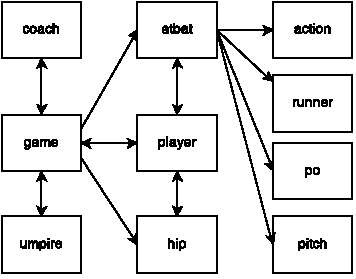
\includegraphics{images/Drawing1.pdf}
\caption{\label{fig:relations}Table relations between Gameday data
accessible via \texttt{scrape()}. The direction of the arrows indicate a
one to possibly many relationship.}
\end{figure}

\section{Introducing XML2R}\label{introducing-xml2r}

\textbf{XML2R} adds to the
\href{http://cran.r-project.org/web/views/WebTechnologies.html}{CRAN Task View on Web Technologies and Services}
by focusing on the transformation of XML content into a collection of
tables. Compared to a lower-level API like the \textbf{XML} package, it
can significantly reduce the amount of coding and cognitive effort
required to perform such a task. In contrast to most higher-level APIs,
it does not make assumptions about the XML structure or its source.
Although \textbf{XML2R} works on any structure, performance and user
experience are enhanced if the content has an inherent relational
structure. \textbf{XML2R}'s novel approach to XML data collection breaks
down the transformation process into a few simple steps and allows the
user to decide how to apply those steps.

The next few sections demonstrate how \textbf{pitchRx} leverages
\textbf{XML2R} in order to produce a collection of tables from
\texttt{inning\_all.xml} files. A similar approach is used by
\texttt{pitchRx::scrape} to construct tables from the other Gameday
files in Table \ref{table:pitchfx}. In fact, \textbf{XML2R} has also
been used in the R package
\href{https://github.com/cpsievert/bbscrapeR}{bbscrapeR} which collects
data from \href{http://nba.com}{nba.com} and
\href{http://wnba.com}{wnba.com}.

\subsection{Constructing file names}\label{constructing-file-names}

Sometimes the most frustrating part of obtaining data in bulk off of the
web is finding the proper collection of URLs or file names of interest.
Since files on the Gameday website are fairly well organized, the
\texttt{makeUrls} function can be used to construct \texttt{urls} that
point to every game's homepage within a window of dates.

\begin{Shaded}
\begin{Highlighting}[]
\NormalTok{urls <-}\StringTok{ }\NormalTok{pitchRx::}\KeywordTok{makeUrls}\NormalTok{(}\DataTypeTok{start =} \StringTok{"2011-06-01"}\NormalTok{, }\DataTypeTok{end =} \StringTok{"2011-06-01"}\NormalTok{) }
\KeywordTok{sub}\NormalTok{(}\StringTok{"http://gd2.mlb.com/components/game/mlb/"}\NormalTok{, }\StringTok{""}\NormalTok{, }\KeywordTok{head}\NormalTok{(urls))}
\CommentTok{#> [1] "year_2011/month_06/day_01/gid_2011_06_01_anamlb_kcamlb_1"}
\CommentTok{#> [2] "year_2011/month_06/day_01/gid_2011_06_01_balmlb_seamlb_1"}
\CommentTok{#> [3] "year_2011/month_06/day_01/gid_2011_06_01_chamlb_bosmlb_1"}
\CommentTok{#> [4] "year_2011/month_06/day_01/gid_2011_06_01_clemlb_tormlb_1"}
\CommentTok{#> [5] "year_2011/month_06/day_01/gid_2011_06_01_colmlb_lanmlb_1"}
\CommentTok{#> [6] "year_2011/month_06/day_01/gid_2011_06_01_flomlb_arimlb_1"}
\end{Highlighting}
\end{Shaded}

\subsection{Extracting observations}\label{extracting-observations}

Once we have a collection of XML \texttt{files}, the next step is to
parse the content into a list of \textit{observations}. An observation
is technically defined as a matrix with one row and some number of
columns. The columns are defined by XML attributes and the XML value (if
any) for a particular XML lineage. The name of each observation tracks
the XML hierarchy so observations can be grouped together in a sensible
fashion at a later point.

\begin{Shaded}
\begin{Highlighting}[]
\KeywordTok{library}\NormalTok{(XML2R)}
\NormalTok{files <-}\StringTok{ }\KeywordTok{paste0}\NormalTok{(urls, }\StringTok{"/inning/inning_all.xml"}\NormalTok{)}
\NormalTok{obs <-}\StringTok{ }\KeywordTok{XML2Obs}\NormalTok{(files, }\DataTypeTok{url.map =} \OtherTok{TRUE}\NormalTok{, }\DataTypeTok{quiet =} \OtherTok{TRUE}\NormalTok{) }
\KeywordTok{table}\NormalTok{(}\KeywordTok{names}\NormalTok{(obs))}
\CommentTok{#> }
\CommentTok{#>                                game }
\CommentTok{#>                                  15 }
\CommentTok{#>                        game//inning }
\CommentTok{#>                                 137 }
\CommentTok{#>        game//inning//bottom//action }
\CommentTok{#>                                 116 }
\CommentTok{#>         game//inning//bottom//atbat }
\CommentTok{#>                                 532 }
\CommentTok{#>  game//inning//bottom//atbat//pitch }
\CommentTok{#>                                1978 }
\CommentTok{#>     game//inning//bottom//atbat//po }
\CommentTok{#>                                  61 }
\CommentTok{#> game//inning//bottom//atbat//runner }
\CommentTok{#>                                 373 }
\CommentTok{#>           game//inning//top//action }
\CommentTok{#>                                 150 }
\CommentTok{#>            game//inning//top//atbat }
\CommentTok{#>                                 593 }
\CommentTok{#>     game//inning//top//atbat//pitch }
\CommentTok{#>                                2183 }
\CommentTok{#>        game//inning//top//atbat//po }
\CommentTok{#>                                  75 }
\CommentTok{#>    game//inning//top//atbat//runner }
\CommentTok{#>                                 509 }
\CommentTok{#>                             url_map }
\CommentTok{#>                                   1}
\end{Highlighting}
\end{Shaded}

This output tells us that 247 pitches were thrown in the bottom inning
and 278 were thrown in the top inning on June 1st, 2011. Also, there are
12 different levels of observations. The list element named
\texttt{url\_map} is not considered an observation and was included
since \texttt{url.map = TRUE}. This helps avoid repeating long file
names in the \texttt{url\_key} column which tracks the mapping between
observations and file names.

\begin{Shaded}
\begin{Highlighting}[]
\NormalTok{obs[}\DecValTok{1}\NormalTok{]}
\CommentTok{#> $`game//inning//top//atbat//pitch`}
\CommentTok{#>      des             des_es           id  type tfs     }
\CommentTok{#> [1,] "Called Strike" "Strike cantado" "3" "S"  "201107"}
\CommentTok{#>      tfs_zulu               x        y        event_num}
\CommentTok{#> [1,] "2011-06-01T20:11:07Z" "103.00" "149.38" "3"      }
\CommentTok{#>      sv_id           play_guid start_speed end_speed sz_top sz_bot}
\CommentTok{#> [1,] "110601_151108" ""        "94.0"      "86.1"    "2.85" "1.36"}
\CommentTok{#>      pfx_x   pfx_z  px       pz      x0       y0     z0      vx0    }
\CommentTok{#> [1,] "-8.12" "11.0" "-0.143" "2.376" "-2.435" "50.0" "5.831" "9.058"}
\CommentTok{#>      vy0        vz0      ax        ay       az        break_y}
\CommentTok{#> [1,] "-137.334" "-7.288" "-15.446" "31.474" "-11.175" "23.8" }
\CommentTok{#>      break_angle break_length pitch_type type_confidence zone nasty}
\CommentTok{#> [1,] "46.3"      "4.0"        "FF"       ".865"          "2"  "46" }
\CommentTok{#>      spin_dir  spin_rate  cc mt url_key}
\CommentTok{#> [1,] "216.336" "2753.789" "" "" "url1"}
\end{Highlighting}
\end{Shaded}

\subsection{Renaming observations}\label{renaming-observations}

Before grouping observations into a collection tables based on their
names, one may want to \texttt{re\_name} observations. Observations with
names \texttt{'game//inning//bottom//atbat'} and
\texttt{'game//inning//top//atbat'} should be included in the same table
since they share XML attributes (in other words, the observations share
variables).

\begin{Shaded}
\begin{Highlighting}[]
\NormalTok{tmp <-}\StringTok{ }\KeywordTok{re_name}\NormalTok{(obs, }\DataTypeTok{equiv =} \KeywordTok{c}\NormalTok{(}\StringTok{"game//inning//top//atbat"}\NormalTok{,                             }
  \StringTok{"game//inning//bottom//atbat"}\NormalTok{), }\DataTypeTok{diff.name =} \StringTok{"inning_side"}\NormalTok{) }
\end{Highlighting}
\end{Shaded}

By passing these names to the \texttt{equiv} argument, \texttt{re\_name}
determines the difference in the naming scheme and suppresses that
difference. In other words, observation names that match the
\texttt{equiv} argument will be renamed to
\texttt{'game//inning//atbat'}. The information removed from the name is
not lost; however, as a new column is appended to the end of each
relevant observation. For example, notice how the \texttt{inning\_side}
column contains the part of the name we just removed:

\begin{Shaded}
\begin{Highlighting}[]
\NormalTok{tmp[}\KeywordTok{grep}\NormalTok{(}\StringTok{"game//inning//atbat"}\NormalTok{, }\KeywordTok{names}\NormalTok{(tmp))][}\DecValTok{1}\NormalTok{:}\DecValTok{2}\NormalTok{]}
\CommentTok{#> $`game//inning//atbat`}
\CommentTok{#>      num b   s   o   start_tfs start_tfs_zulu         batter   stand}
\CommentTok{#> [1,] "1" "3" "2" "0" "201034"  "2011-06-01T20:10:34Z" "430947" "L"  }
\CommentTok{#>      b_height pitcher  p_throws}
\CommentTok{#> [1,] "5-10"   "462956" "R"     }
\CommentTok{#>      des                                                                     }
\CommentTok{#> [1,] "Erick Aybar singles on a line drive to center fielder Melky Cabrera.  "}
\CommentTok{#>      des_es                                                                    }
\CommentTok{#> [1,] "Erick Aybar pega sencillo con línea a jardinero central Melky Cabrera.  "}
\CommentTok{#>      event_num event    event_es   home_team_runs away_team_runs}
\CommentTok{#> [1,] "12"      "Single" "Sencillo" "0"            "0"           }
\CommentTok{#>      url_key inning_side}
\CommentTok{#> [1,] "url1"  "top"      }
\CommentTok{#> }
\CommentTok{#> $`game//inning//atbat`}
\CommentTok{#>      num b   s   o   start_tfs start_tfs_zulu         batter   stand}
\CommentTok{#> [1,] "2" "2" "3" "1" "201412"  "2011-06-01T20:14:12Z" "110029" "L"  }
\CommentTok{#>      b_height pitcher  p_throws}
\CommentTok{#> [1,] "6-0"    "462956" "R"     }
\CommentTok{#>      des                                   }
\CommentTok{#> [1,] "Bobby Abreu called out on strikes.  "}
\CommentTok{#>      des_es                                 event_num event      }
\CommentTok{#> [1,] "Bobby Abreu se poncha sin tirarle.  " "24"      "Strikeout"}
\CommentTok{#>      event_es home_team_runs away_team_runs url_key inning_side}
\CommentTok{#> [1,] "Ponche" "0"            "0"            "url1"  "top"}
\end{Highlighting}
\end{Shaded}

For similar reasons, other observation name pairs are renamed in a
similar fashion.

\begin{Shaded}
\begin{Highlighting}[]
\NormalTok{tmp <-}\StringTok{ }\KeywordTok{re_name}\NormalTok{(tmp, }\DataTypeTok{equiv =} \KeywordTok{c}\NormalTok{(}\StringTok{"game//inning//top//atbat//runner"}\NormalTok{,                             }
  \StringTok{"game//inning//bottom//atbat//runner"}\NormalTok{), }\DataTypeTok{diff.name =} \StringTok{"inning_side"}\NormalTok{)}
\NormalTok{tmp <-}\StringTok{ }\KeywordTok{re_name}\NormalTok{(tmp, }\DataTypeTok{equiv =} \KeywordTok{c}\NormalTok{(}\StringTok{"game//inning//top//action"}\NormalTok{,                             }
  \StringTok{"game//inning//bottom//action"}\NormalTok{), }\DataTypeTok{diff.name =} \StringTok{"inning_side"}\NormalTok{)  }
\NormalTok{tmp <-}\StringTok{ }\KeywordTok{re_name}\NormalTok{(tmp, }\DataTypeTok{equiv =} \KeywordTok{c}\NormalTok{(}\StringTok{"game//inning//top//atbat//po"}\NormalTok{,                            }
  \StringTok{"game//inning//bottom//atbat//po"}\NormalTok{), }\DataTypeTok{diff.name =} \StringTok{"inning_side"}\NormalTok{)}
\NormalTok{obs2 <-}\StringTok{ }\KeywordTok{re_name}\NormalTok{(tmp, }\DataTypeTok{equiv =} \KeywordTok{c}\NormalTok{(}\StringTok{"game//inning//top//atbat//pitch"}\NormalTok{,                             }
  \StringTok{"game//inning//bottom//atbat//pitch"}\NormalTok{), }\DataTypeTok{diff.name =} \StringTok{"inning_side"}\NormalTok{) }
\KeywordTok{table}\NormalTok{(}\KeywordTok{names}\NormalTok{(obs2))}
\CommentTok{#> }
\CommentTok{#>                        game                game//inning }
\CommentTok{#>                          15                         137 }
\CommentTok{#>        game//inning//action         game//inning//atbat }
\CommentTok{#>                         266                        1125 }
\CommentTok{#>  game//inning//atbat//pitch     game//inning//atbat//po }
\CommentTok{#>                        4161                         136 }
\CommentTok{#> game//inning//atbat//runner                     url_map }
\CommentTok{#>                         882                           1}
\end{Highlighting}
\end{Shaded}

\subsection{Linking observations}\label{linking-observations}

After all that renaming, we now have 7 different levels of observations.
Let's examine the first three observations on the \texttt{game//inning}
level:

\begin{Shaded}
\begin{Highlighting}[]
\NormalTok{obs2[}\KeywordTok{grep}\NormalTok{(}\StringTok{"^game//inning$"}\NormalTok{, }\KeywordTok{names}\NormalTok{(obs2))][}\DecValTok{1}\NormalTok{:}\DecValTok{3}\NormalTok{] }
\CommentTok{#> $`game//inning`}
\CommentTok{#>      num away_team home_team next url_key}
\CommentTok{#> [1,] "1" "ana"     "kca"     "Y"  "url1" }
\CommentTok{#> }
\CommentTok{#> $`game//inning`}
\CommentTok{#>      num away_team home_team next url_key}
\CommentTok{#> [1,] "2" "ana"     "kca"     "Y"  "url1" }
\CommentTok{#> }
\CommentTok{#> $`game//inning`}
\CommentTok{#>      num away_team home_team next url_key}
\CommentTok{#> [1,] "3" "ana"     "kca"     "Y"  "url1"}
\end{Highlighting}
\end{Shaded}

Before grouping observations into tables, it is usually important
preserve the parent-to-child relationships in the XML lineage. For
example, one may want to map a particular pitch back to the inning in
which it was thrown. Using the \texttt{add\_key} function, the relevant
value of \texttt{num} for \texttt{game//inning} observations can be
\texttt{recycle}d to its XML descendants.

\begin{Shaded}
\begin{Highlighting}[]
\NormalTok{obswkey <-}\StringTok{ }\KeywordTok{add_key}\NormalTok{(obs2, }\DataTypeTok{parent =} \StringTok{"game//inning"}\NormalTok{, }\DataTypeTok{recycle =} \StringTok{"num"}\NormalTok{, }\DataTypeTok{key.name =} \StringTok{"inning"}\NormalTok{)}
\end{Highlighting}
\end{Shaded}

As it turns out, the \texttt{away\_team} and \texttt{home\_team} columns
are redundant as this information is embedded in the \texttt{url}
column. Thus, there is only one other informative attribute on this
level which is \texttt{next}. By recycling this value among its
descendants, we remove any need to retain a \texttt{game//inning} table.

\begin{Shaded}
\begin{Highlighting}[]
\NormalTok{obswkey <-}\StringTok{ }\KeywordTok{add_key}\NormalTok{(obswkey, }\DataTypeTok{parent =} \StringTok{"game//inning"}\NormalTok{, }\DataTypeTok{recycle =} \StringTok{"next"}\NormalTok{)}
\end{Highlighting}
\end{Shaded}

It is also imperative that we can link a \texttt{pitch},
\texttt{runner}, or \texttt{po} back to a particular \texttt{atbat}.
This can be done as follows:

\begin{Shaded}
\begin{Highlighting}[]
\NormalTok{obswkey <-}\StringTok{ }\KeywordTok{add_key}\NormalTok{(obswkey, }\DataTypeTok{parent =} \StringTok{"game//inning//atbat"}\NormalTok{, }\DataTypeTok{recycle =} \StringTok{"num"}\NormalTok{)}
\end{Highlighting}
\end{Shaded}

\subsection{Collapsing observations}\label{collapsing-observations}

Finally, we are in a position to pool together observations that have a
common name. The \texttt{collapse\_obs} function achieves this by row
binding observations with the same name together and returning a list of
matrices. Note that \texttt{collapse\_obs} does not require that
observations from the same level to have the same set of variables in
order to be bound into a common table. In the case where variables are
missing, \texttt{NA}s will be inserted as values.

\begin{Shaded}
\begin{Highlighting}[]
\NormalTok{tables <-}\StringTok{ }\KeywordTok{collapse_obs}\NormalTok{(obswkey) }
\CommentTok{#As mentioned before, we do not need the 'inning' table }
\NormalTok{tables <-}\StringTok{ }\NormalTok{tables[!}\KeywordTok{grepl}\NormalTok{(}\StringTok{"^game//inning$"}\NormalTok{, }\KeywordTok{names}\NormalTok{(tables))]      }
\NormalTok{table.names <-}\StringTok{ }\KeywordTok{c}\NormalTok{(}\StringTok{"game"}\NormalTok{, }\StringTok{"action"}\NormalTok{, }\StringTok{"atbat"}\NormalTok{, }\StringTok{"pitch"}\NormalTok{, }\StringTok{"po"}\NormalTok{, }\StringTok{"runner"}\NormalTok{) }
\NormalTok{tables <-}\StringTok{ }\KeywordTok{setNames}\NormalTok{(tables, table.names) }
\KeywordTok{head}\NormalTok{(tables[[}\StringTok{"runner"}\NormalTok{]])}
\CommentTok{#>      id       start end  event                event_num url_key}
\CommentTok{#> [1,] "430947" ""    "1B" "Single"             "12"      "url1" }
\CommentTok{#> [2,] "430947" "1B"  "2B" "Stolen Base 2B"     "19"      "url1" }
\CommentTok{#> [3,] "430947" "2B"  "3B" "Groundout"          "30"      "url1" }
\CommentTok{#> [4,] "430947" "3B"  ""   "Groundout"          "36"      "url1" }
\CommentTok{#> [5,] "543333" ""    "1B" "Single"             "58"      "url1" }
\CommentTok{#> [6,] "543333" "1B"  ""   "Pickoff Attempt 1B" "69"      "url1" }
\CommentTok{#>      inning_side inning next num score rbi earned}
\CommentTok{#> [1,] "top"       "1"    "Y"  "1" NA    NA  NA    }
\CommentTok{#> [2,] "top"       "1"    "Y"  "2" NA    NA  NA    }
\CommentTok{#> [3,] "top"       "1"    "Y"  "3" NA    NA  NA    }
\CommentTok{#> [4,] "top"       "1"    "Y"  "4" NA    NA  NA    }
\CommentTok{#> [5,] "bottom"    "1"    "Y"  "7" NA    NA  NA    }
\CommentTok{#> [6,] "bottom"    "1"    "Y"  "8" NA    NA  NA}
\end{Highlighting}
\end{Shaded}

\section{Collecting Gameday data with
pitchRx}\label{collecting-gameday-data-with-pitchrx}

The main scraping function in \textbf{pitchRx}, \texttt{scrape}, can be
used to easily obtain data from the files listed in Table
\ref{table:pitchfx}. In fact, any combination of these files can be
queried using the \texttt{suffix} argument. In the example below, the
\texttt{start} and \texttt{end} arguments are also used so that all
available file types for June 1st, 2011 are queried.

\begin{Shaded}
\begin{Highlighting}[]
\KeywordTok{library}\NormalTok{(pitchRx)}
\NormalTok{files <-}\StringTok{ }\KeywordTok{c}\NormalTok{(}\StringTok{"inning/inning_all.xml"}\NormalTok{, }\StringTok{"inning/inning_hit.xml"}\NormalTok{, }
  \StringTok{"miniscoreboard.xml"}\NormalTok{, }\StringTok{"players.xml"}\NormalTok{)}
\NormalTok{dat <-}\StringTok{ }\KeywordTok{scrape}\NormalTok{(}\DataTypeTok{start =} \StringTok{"2011-06-01"}\NormalTok{, }\DataTypeTok{end =} \StringTok{"2011-06-01"}\NormalTok{, }\DataTypeTok{suffix =} \NormalTok{files)}
\end{Highlighting}
\end{Shaded}

The \texttt{game.ids} option can be used instead of \texttt{start} and
\texttt{end} to obtain an equivalent \texttt{dat} object. This option
can be useful if the user wants to query specific games rather than all
games played over a particular time span. When using this
\texttt{game.ids} option, the built-in \texttt{gids} object, is quite
convenient.

\begin{Shaded}
\begin{Highlighting}[]
\KeywordTok{data}\NormalTok{(gids, }\DataTypeTok{package =} \StringTok{"pitchRx"}\NormalTok{)}
\NormalTok{gids11 <-}\StringTok{ }\NormalTok{gids[}\KeywordTok{grep}\NormalTok{(}\StringTok{"2011_06_01"}\NormalTok{, gids)]}
\KeywordTok{head}\NormalTok{(gids11)}
\CommentTok{#> [1] "gid_2011_06_01_anamlb_kcamlb_1" "gid_2011_06_01_balmlb_seamlb_1"}
\CommentTok{#> [3] "gid_2011_06_01_chamlb_bosmlb_1" "gid_2011_06_01_clemlb_tormlb_1"}
\CommentTok{#> [5] "gid_2011_06_01_colmlb_lanmlb_1" "gid_2011_06_01_flomlb_arimlb_1"}
\end{Highlighting}
\end{Shaded}

\begin{Shaded}
\begin{Highlighting}[]
\NormalTok{dat <-}\StringTok{ }\KeywordTok{scrape}\NormalTok{(}\DataTypeTok{game.ids =} \NormalTok{gids11, }\DataTypeTok{suffix =} \NormalTok{files)}
\end{Highlighting}
\end{Shaded}

The object \texttt{dat} is a list of data frames containing all data
available for June 1st, 2011 using \texttt{scrape}. The list names match
the table names provided in Table \ref{table:pitchfx}. For example,
\texttt{dat\$atbat} is data frame with every at bat on June 1st, 2011
and \texttt{dat\$pitch} has information related to the outcome of each
pitch (including PITCHf/x parameters). The \texttt{object.size} of
\texttt{dat} is nearly 300MB. Multiplying this number by 100 days
exceeds the memory of most machines. Thus, if a large amount of data is
required, the user should exploit the R database interface (R Special
Interest Group on Databases \protect\hyperlink{ref-DBI}{2013}).

\section{Storing and querying Gameday
data}\label{storing-and-querying-gameday-data}

Since PITCHf/x data can easily exhaust memory, one should consider
establishing a database instance before using \texttt{scrape}. By
passing a database connection to the \texttt{connect} argument,
\texttt{scrape} will try to create (and/or append to existing) tables
using that connection. If the connection fails for some reason, tables
will be written as csv files in the current working directory. The
benefits of using the \texttt{connect} argument includes improved memory
management which can greatly reduce run time. \texttt{connect} will
support a MySQL connection, but creating a SQLite database is quite easy
with \textbf{dplyr} (Wickham and Francois
\protect\hyperlink{ref-dplyr}{2014}).

\begin{Shaded}
\begin{Highlighting}[]
\KeywordTok{library}\NormalTok{(dplyr)}
\NormalTok{db <-}\StringTok{ }\KeywordTok{src_sqlite}\NormalTok{(}\StringTok{"GamedayDB.sqlite3"}\NormalTok{, }\DataTypeTok{create =} \OtherTok{TRUE}\NormalTok{)}
\CommentTok{# Collect and store all PITCHf/x data from 2008 to now}
\KeywordTok{scrape}\NormalTok{(}\DataTypeTok{start =} \StringTok{"2008-01-01"}\NormalTok{, }\DataTypeTok{end =} \KeywordTok{Sys.Date}\NormalTok{(), }
  \DataTypeTok{suffix =} \StringTok{"inning/inning_all.xml"}\NormalTok{, }\DataTypeTok{connect =} \NormalTok{db$con)}
\end{Highlighting}
\end{Shaded}

In the later sections, animations of four-seam and cut fastballs thrown
by Mariano Rivera and Phil Hughes during the 2011 season are created. In
order to obtain the data for those animations, one could query
\texttt{db} which now has PITCHf/x data from 2008 to date. This query
requires criteria on: the \texttt{pitcher\_name} field (in the
\texttt{atbat} table), the \texttt{pitch\_type} field (in the
\texttt{pitch} table), and the \texttt{date} field (in both tables). To
reduce the time required to search those records, one should create an
index on each of these three fields.

\begin{Shaded}
\begin{Highlighting}[]
\KeywordTok{library}\NormalTok{(DBI)}
\KeywordTok{dbSendQuery}\NormalTok{(db$con, }\StringTok{"CREATE INDEX pitcher_index ON atbat(pitcher_name)"}\NormalTok{) }
\KeywordTok{dbSendQuery}\NormalTok{(db$con, }\StringTok{"CREATE INDEX type_index ON pitch(pitch_type)"}\NormalTok{) }
\KeywordTok{dbSendQuery}\NormalTok{(db$con, }\StringTok{"CREATE INDEX date_atbat ON atbat(date)"}\NormalTok{) }
\end{Highlighting}
\end{Shaded}

As a part of our query, we'll have to join the \texttt{atbat} table
together with the \texttt{pitch} table. For this task, the
\texttt{gameday\_link} and \texttt{num} fields are helpful since
together they provide a way to match pitches with at bats. For this
reason, a multi-column index on the \texttt{gameday\_link} and
\texttt{num} fields will further reduce run time of the query.

\begin{Shaded}
\begin{Highlighting}[]
\KeywordTok{dbSendQuery}\NormalTok{(db$con, }\StringTok{'CREATE INDEX pitch_join ON pitch(gameday_link, num)'}\NormalTok{) }
\KeywordTok{dbSendQuery}\NormalTok{(db$con, }\StringTok{'CREATE INDEX atbat_join ON atbat(gameday_link, num)'}\NormalTok{)}
\end{Highlighting}
\end{Shaded}

Although the query itself could be expressed entirely in SQL,
\textbf{dplyr}'s grammar for data manipulation (which is database
agnostic) can help to simplify the task. In this case, \texttt{at.bat}
is a tabular \emph{representation} of the remote \texttt{atbat} table
restricted to cases where Rivera or Hughes was the pitcher. That is,
\texttt{at.bat} does not contain the actual data, but it does contain
the information necessary to retrieve it from the database.

\begin{Shaded}
\begin{Highlighting}[]
\NormalTok{at.bat <-}\StringTok{ }\KeywordTok{tbl}\NormalTok{(db, }\StringTok{"atbat"}\NormalTok{) %>%}\StringTok{   }
\StringTok{  }\KeywordTok{filter}\NormalTok{(pitcher_name %in%}\StringTok{ }\KeywordTok{c}\NormalTok{(}\StringTok{"Mariano Rivera"}\NormalTok{, }\StringTok{"Phil Hughes"}\NormalTok{))}
\end{Highlighting}
\end{Shaded}

Similarly, \texttt{fbs} is a tabular representation of the
\texttt{pitch} table restricted to four-seam (FF) and cut fastballs
(FC).

\begin{Shaded}
\begin{Highlighting}[]
\NormalTok{fbs <-}\StringTok{ }\KeywordTok{tbl}\NormalTok{(db, }\StringTok{"pitch"}\NormalTok{) %>%}\StringTok{      }
\StringTok{  }\KeywordTok{filter}\NormalTok{(pitch_type %in%}\StringTok{ }\KeywordTok{c}\NormalTok{(}\StringTok{"FF"}\NormalTok{, }\StringTok{"FC"}\NormalTok{))}
\end{Highlighting}
\end{Shaded}

An \texttt{inner\_join} of these two filtered tables returns a tabular
representation of all four-seam and cut fastballs thrown by Rivera and
Hughes. Before \texttt{collect} actually performs the database query and
brings the relevant data into the R session, another restriction is
added so that only pitches from 2011 are included.

\begin{Shaded}
\begin{Highlighting}[]
\NormalTok{pitches <-}\StringTok{ }\KeywordTok{inner_join}\NormalTok{(fbs, at.bat) %>%}\StringTok{ }
\StringTok{  }\KeywordTok{filter}\NormalTok{(date >=}\StringTok{ "2011_01_01"} \NormalTok{&}\StringTok{ }\NormalTok{date <=}\StringTok{ "2012_01_01"}\NormalTok{) %>%}
\StringTok{  }\KeywordTok{collect}\NormalTok{()}
\end{Highlighting}
\end{Shaded}

\section{Visualizing PITCHf/x}\label{visualizing-pitchfx}

\subsection{Strike-zone plots and umpire
bias}\label{strike-zone-plots-and-umpire-bias}

Amongst the most common PITCHf/x graphics are strike-zone plots. Such a
plot has two axes and the coordinates represent the location of
baseballs as they cross home plate. The term strike-zone plot can refer
to either \emph{density} or \emph{probabilistic} plots. Density plots
are useful for exploring what \emph{actually} occurred, but
probabilistic plots can help address much more interesting questions
using statistical inference. Although probabilistic plots can be used to
visually track any event probability across the strike-zone, their most
popular use is for addressing umpire bias in a strike versus ball
decision (Green and Daniels \protect\hyperlink{ref-bias}{2014}). The
probabilistic plots section demonstrates how \textbf{pitchRx} simplifies
the process behind creating such plots via a case study on the impact of
home field advantage on umpire decisions.

In the world of sports, it is a common belief that umpires (or referees)
have a tendency to favor the home team. PITCHf/x provides a unique
opportunity to add to this discussion by modeling the probability of a
called strike at home games versus away games. Specifically, conditioned
upon the umpire making a decision at a specific location in the
strike-zone, if the probability that a home pitcher receives a called
strike is higher than the probability that an away pitcher receives a
called strike, then there is evidence to support umpire bias towards a
home pitcher.

There are many different possible outcomes of each pitch, but we can
condition on the umpire making a decision by limiting to the following
two cases. A \textit{called strike} is an outcome of a pitch where the
batter does not swing and the umpire declares the pitch a strike (which
is a favorable outcome for the pitcher). A \textit{ball} is another
outcome where the batter does not swing and the umpire declares the
pitch a ball (which is a favorable outcome for the batter). All
\texttt{decisions} made between 2008 and 2013 can be obtained from
\texttt{db} with the following query using \textbf{dplyr}.

\begin{Shaded}
\begin{Highlighting}[]
\CommentTok{# First, add an index on the pitch description to speed up run-time}
\KeywordTok{dbSendQuery}\NormalTok{(db$con, }\StringTok{"CREATE INDEX des_index ON pitch(des)"}\NormalTok{)}

\NormalTok{pitch <-}\StringTok{ }\KeywordTok{tbl}\NormalTok{(db, }\StringTok{"pitch"}\NormalTok{) %>%}\StringTok{   }
\StringTok{  }\KeywordTok{filter}\NormalTok{(des %in%}\StringTok{ }\KeywordTok{c}\NormalTok{(}\StringTok{"Called Strike"}\NormalTok{, }\StringTok{"Ball"}\NormalTok{)) %>%}\StringTok{   }
\StringTok{  }\CommentTok{# Keep pitch location, descriptions    }
\StringTok{  }\KeywordTok{select}\NormalTok{(px, pz, des, gameday_link, num) %>%}\StringTok{   }
\StringTok{  }\CommentTok{# 0-1 indicator of strike/ball   }
\StringTok{  }\KeywordTok{mutate}\NormalTok{(}\DataTypeTok{strike =} \KeywordTok{as.numeric}\NormalTok{(des ==}\StringTok{ "Called Strike"}\NormalTok{))}

\NormalTok{atbat <-}\StringTok{ }\KeywordTok{tbl}\NormalTok{(db, }\StringTok{"atbat"}\NormalTok{) %>%}\StringTok{   }
\StringTok{  }\CommentTok{# Select variables to be used later as covariates in probabilistic models}
\StringTok{  }\KeywordTok{select}\NormalTok{(b_height, p_throws, stand, inning_side, date, gameday_link, num)    }

\NormalTok{decisions <-}\StringTok{ }\KeywordTok{inner_join}\NormalTok{(pitch, atbat) %>%}\StringTok{   }
\StringTok{  }\KeywordTok{filter}\NormalTok{(date <=}\StringTok{ "2014_01_01"}\NormalTok{) %>%}\StringTok{   }
\StringTok{  }\KeywordTok{collect}\NormalTok{()}
\end{Highlighting}
\end{Shaded}

\subsubsection{Density plots}

The \texttt{decisions} data frame contains data on over 2.5 million
pitches thrown from 2008 to 2013. About a third of them are called
strikes and two-thirds balls. Figure \ref{fig:STRIKES} shows the density
of all called strikes. Clearly, most called strikes occur on the outer
region of the strike-zone. Many factors could contribute to this
phenomenon; which we will not investigate here.

\begin{Shaded}
\begin{Highlighting}[]
\CommentTok{# strikeFX uses the stand variable to calculate strike-zones }
\CommentTok{# Here is a slick way to create better facet titles without changing data values}
\NormalTok{relabel <-}\StringTok{ }\NormalTok{function(variable, value) \{ }
  \NormalTok{value <-}\StringTok{ }\KeywordTok{sub}\NormalTok{(}\StringTok{"^R$"}\NormalTok{, }\StringTok{"Right-Handed Batter"}\NormalTok{, value) }
  \KeywordTok{sub}\NormalTok{(}\StringTok{"^L$"}\NormalTok{, }\StringTok{"Left-Handed Batter"}\NormalTok{, value) }
\NormalTok{\}}
\NormalTok{strikes <-}\StringTok{ }\KeywordTok{subset}\NormalTok{(decisions, strike ==}\StringTok{ }\DecValTok{1}\NormalTok{)}
\KeywordTok{strikeFX}\NormalTok{(strikes, }\DataTypeTok{geom =} \StringTok{"raster"}\NormalTok{, }\DataTypeTok{layer =} \KeywordTok{facet_grid}\NormalTok{(. ~}\StringTok{ }\NormalTok{stand, }\DataTypeTok{labeller =} \NormalTok{relabel))}
\end{Highlighting}
\end{Shaded}

\begin{figure}
\centering
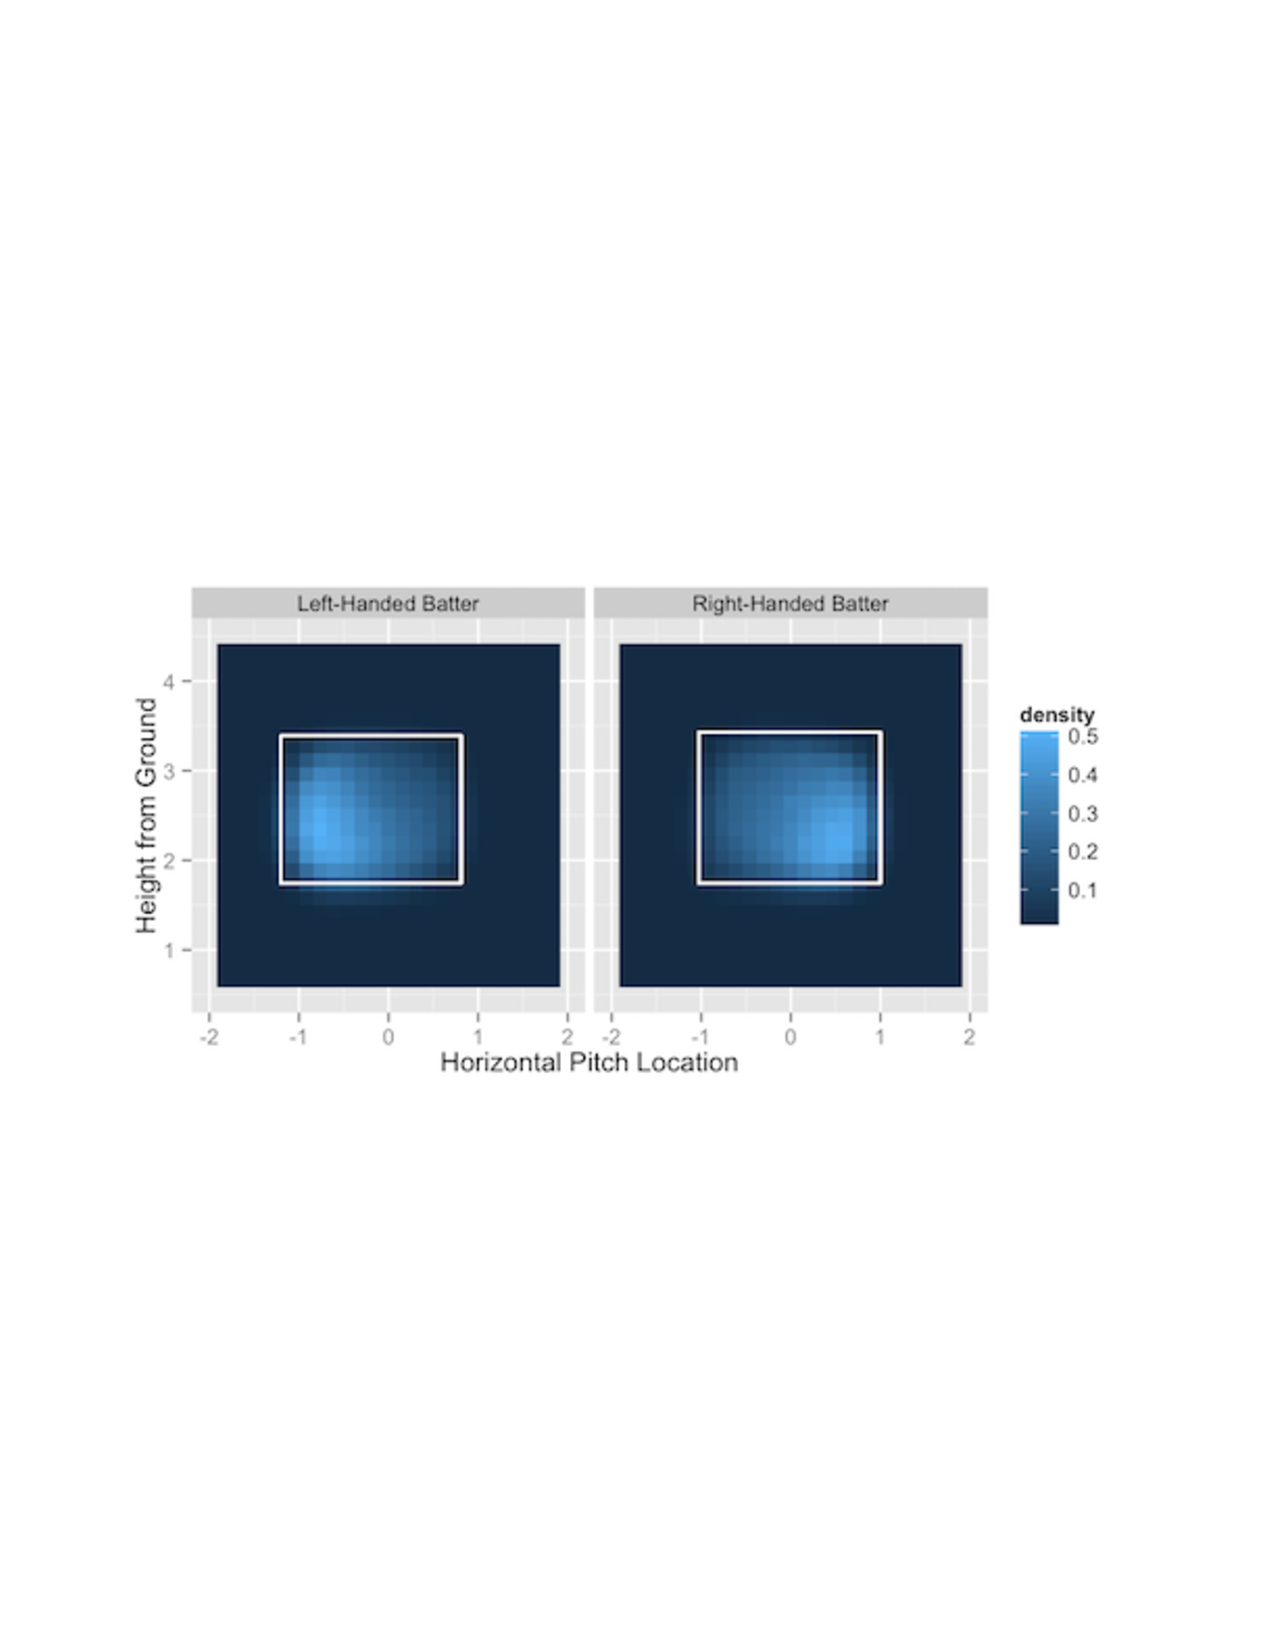
\includegraphics{images/strikes.pdf}
\caption{\label{fig:STRIKES}Density of called strikes for right-handed
batters and left-handed batters (from 2008 to 2013).}
\end{figure}

Figure \ref{fig:STRIKES} shows one static rectangle (or strike-zone) per
plot automatically generated by \texttt{strikeFX}. The definition of the
strike-zone is notoriously ambiguous. As a result, the boundaries of the
strike-zone may be noticeably different in some situations. However, we
can achieve a fairly accurate representation of strike-zones using a
rectangle defined by batters' average height and stance (Fast
\protect\hyperlink{ref-Strikezones}{2011}). As Figure
\ref{fig:strike-probs} reinforces, batter stance makes an important
difference since the strike-zone seems to be horizontally shifted away
from the batter. The batter's height is also important since the
strike-zone is classically defined as approximately between the batter's
knees and armpits.

Figure \ref{fig:STRIKES} has is one strike-zone per plot since the
\texttt{layer} option contains a \textbf{ggplot2} argument that facets
according to batter stance. Facet layers are a powerful tool for
analyzing PITCHf/x data because they help produce quick and insightful
comparisons. In addition to using the \texttt{layer} option, one can add
layers to a graphic returned by \texttt{strikeFX} using \textbf{ggplot2}
arithmetic. It is also worth pointing out that Figure \ref{fig:STRIKES}
could have been created without introducing the \texttt{strikes} data
frame by using the \texttt{density1} and \texttt{density2} options.

\begin{Shaded}
\begin{Highlighting}[]
\KeywordTok{strikeFX}\NormalTok{(decisions, }\DataTypeTok{geom =} \StringTok{"raster"}\NormalTok{, }\DataTypeTok{density1 =} \KeywordTok{list}\NormalTok{(}\DataTypeTok{des =} \StringTok{"Called Strike"}\NormalTok{),          }
  \DataTypeTok{density2 =} \KeywordTok{list}\NormalTok{(}\DataTypeTok{des =} \StringTok{"Called Strike"}\NormalTok{)) +}\StringTok{ }\KeywordTok{facet_grid}\NormalTok{(. ~}\StringTok{ }\NormalTok{stand, }\DataTypeTok{labeller =} \NormalTok{relabel)}
\end{Highlighting}
\end{Shaded}

In general, when \texttt{density1} and \texttt{density2} are identical,
the result is equivalent to subsetting the data frame appropriately
beforehand. More importantly, by specifying \emph{different} values for
\texttt{density1} and \texttt{density2}, differenced densities are
easily generated. In this case, a grid of density estimates for
\texttt{density2} are subtracted from the corresponding grid of density
estimates for \texttt{density1}. Note that the default \texttt{NULL}
value for either density option infers that the entire data set defines
the relevant density. Thus, if \texttt{density2} was \texttt{NULL} (when
\texttt{density1 = list(des = 'Called Strike')}), we would obtain the
density of called strikes minus the density of \emph{both} called
strikes and balls. In Figure \ref{fig:strikesVSballs}, we define
\texttt{density1} as called strikes and define \texttt{density2} as
balls. As expected, we see positive density values (in blue) inside the
strike-zone and negative density values (in red) outside of the
strike-zone.

\begin{Shaded}
\begin{Highlighting}[]
\KeywordTok{strikeFX}\NormalTok{(decisions, }\DataTypeTok{geom =} \StringTok{"raster"}\NormalTok{, }\DataTypeTok{density1 =} \KeywordTok{list}\NormalTok{(}\DataTypeTok{des =} \StringTok{"Called Strike"}\NormalTok{), }
  \DataTypeTok{density2 =} \KeywordTok{list}\NormalTok{(}\DataTypeTok{des =} \StringTok{"Ball"}\NormalTok{), }\DataTypeTok{layer =} \KeywordTok{facet_grid}\NormalTok{(. ~}\StringTok{ }\NormalTok{stand, }\DataTypeTok{labeller =} \NormalTok{relabel)) }
\end{Highlighting}
\end{Shaded}

\begin{figure}
\centering
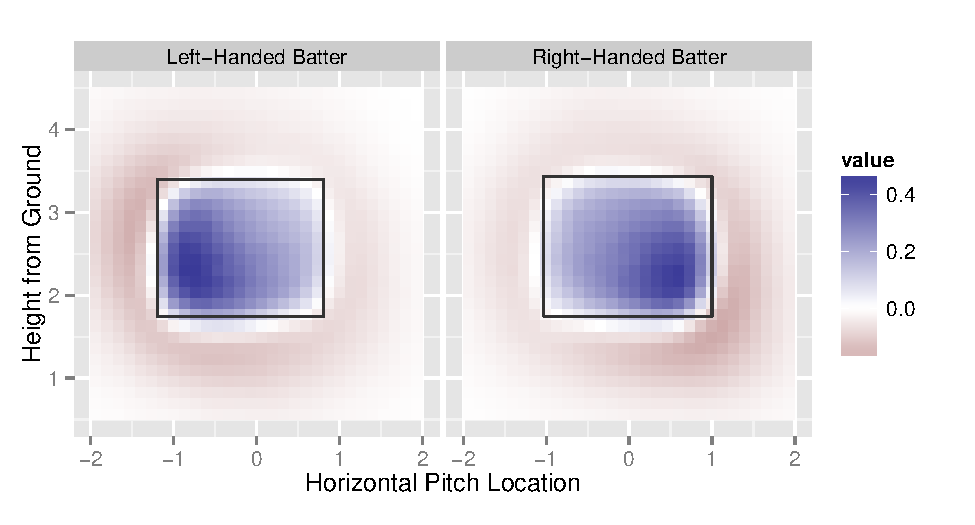
\includegraphics{images/strikesVSballs.pdf}
\caption{\label{fig:strikesVSballs}Density of called strikes minus density
of balls for both right-handed batters and left-handed batters (from
2008 to 2013). The blue region indicates a higher frequency of called
strikes and the red region indicates a higher frequency of balls.}
\end{figure}

These density plots are helpful for visualizing the observed frequency
of events; however, they are not very useful for addressing our umpire
bias hypothesis. Instead of looking simply at the \emph{density}, we
want to model the \emph{probability} of a strike called at each
coordinate given the umpire has to make a decision.

\subsubsection{Probabilistic plots}

There are many approaches to probabilistic modeling over a two
dimensional spatial region. Since our response is often categorical,
generalized additive models (GAMs) is a popular and desirable approach
to modeling events over the strike-zone (Mills
\protect\hyperlink{ref-loess}{2010}). There are numerous R package
implementations of GAMs, but the \texttt{bam} function from the
\textbf{mgcv} package has several desirable properties (Wood
\protect\hyperlink{ref-mgcv}{2006}). Most importantly, the smoothing
parameter can be estimated using several different methods. In order to
have a reasonable estimate of the smooth 2D surface, GAMs require fairly
large amount of observations. As a result, run time can be an issue --
especially when modeling 2.5 million observations! Thankfully, the
\texttt{bam} function has a \texttt{cluster} argument which allows one
to distribute computations across multiple cores using the built in
\textbf{parallel} package.

\begin{Shaded}
\begin{Highlighting}[]
\KeywordTok{library}\NormalTok{(parallel) }
\NormalTok{cl <-}\StringTok{ }\KeywordTok{makeCluster}\NormalTok{(}\KeywordTok{detectCores}\NormalTok{() -}\StringTok{ }\DecValTok{1}\NormalTok{)}
\KeywordTok{library}\NormalTok{(mgcv) }
\NormalTok{m <-}\StringTok{ }\KeywordTok{bam}\NormalTok{(strike ~}\StringTok{ }\KeywordTok{interaction}\NormalTok{(stand, p_throws, inning_side) +}\StringTok{                }
\StringTok{  }\KeywordTok{s}\NormalTok{(px, pz, }\DataTypeTok{by =} \KeywordTok{interaction}\NormalTok{(stand, p_throws, inning_side)),              }
  \DataTypeTok{data =} \NormalTok{decisions, }\DataTypeTok{family =} \KeywordTok{binomial}\NormalTok{(}\DataTypeTok{link =} \StringTok{'logit'}\NormalTok{), }\DataTypeTok{cluster =} \NormalTok{cl)}
\end{Highlighting}
\end{Shaded}

This formula models the probability of a strike as a function of the
baseball's spatial location, the batter's stance, the pitcher's throwing
arm, and the side of the inning. Since home pitchers always pitch during
the top of the inning, \texttt{inning\_side} also serves as an
indication of whether a pitch is thrown by a home pitcher. In this case,
the \texttt{interaction} function creates a factor with eight different
levels since every input factor has two levels. Consequently, there are
8 different levels of smooth surfaces over the spatial region defined by
\texttt{px} and \texttt{pz}.

The fitted model \texttt{m} contains a lot of information which
\texttt{strikeFX} uses in conjunction with any \textbf{ggplot2} facet
commands to infer which and how surfaces should be plotted. In
particular, the \texttt{var.summary} is used to identify model
covariates, as well their default conditioning values. In our case, the
majority of \texttt{decisions} are from right-handed pitchers and the
top of the inning. Thus, the default conditioning values are
\texttt{"top"} for \texttt{inning\_side} and \texttt{"R"} for
\texttt{p\_throws}. If different conditioning values are desired,
\texttt{var.summary} can be modified accordingly. To demonstrate, Figure
\ref{fig:strike-probs} shows 2 of the 8 possible surfaces that
correspond to a right-handed \emph{away} pitcher.

\begin{Shaded}
\begin{Highlighting}[]
\NormalTok{away <-}\StringTok{ }\KeywordTok{list}\NormalTok{(}\DataTypeTok{inning_side =} \KeywordTok{factor}\NormalTok{(}\StringTok{"bottom"}\NormalTok{, }\DataTypeTok{levels =} \KeywordTok{c}\NormalTok{(}\StringTok{"top"}\NormalTok{, }\StringTok{"bottom"}\NormalTok{)))}
\NormalTok{m$var.summary <-}\StringTok{ }\KeywordTok{modifyList}\NormalTok{(m$var.summary, away)}
\KeywordTok{strikeFX}\NormalTok{(decisions, }\DataTypeTok{model =} \NormalTok{m, }\DataTypeTok{layer =} \KeywordTok{facet_grid}\NormalTok{(. ~}\StringTok{ }\NormalTok{stand, }\DataTypeTok{labeller =} \NormalTok{relabel))}
\end{Highlighting}
\end{Shaded}

\begin{figure}
\centering
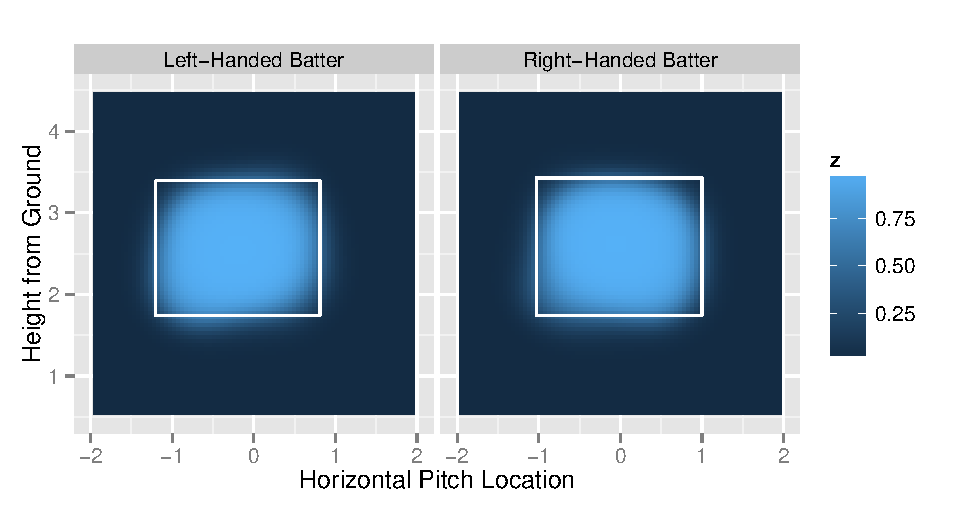
\includegraphics{images/prob-strike.pdf}
\caption{\label{fig:strike-probs}Probability that a right-handed away
pitcher receives a called strike (provided the umpire has to make a
decision). Plots are faceted by the handedness of the batter.}
\end{figure}

Using the same intuition exploited earlier to obtain differenced density
plots, we can easily obtain differenced probability plots. To obtain
Figure \ref{fig:diff-probs}, we simply add \texttt{p\_throws} as another
facet variable and \texttt{inning\_side} as a differencing variable. In
this case, conditioning values do not matter since every one of the 8
surfaces are required in order to produce Figure \ref{fig:diff-probs}.

\begin{Shaded}
\begin{Highlighting}[]
\CommentTok{# Function to create better labels for both stand and p_throws}
\NormalTok{relabel2 <-}\StringTok{ }\NormalTok{function(variable, value) \{    }
  \NormalTok{if (variable %in%}\StringTok{ "stand"}\NormalTok{)      }
    \KeywordTok{return}\NormalTok{(}\KeywordTok{sub}\NormalTok{(}\StringTok{"^L$"}\NormalTok{, }\StringTok{"Left-Handed Batter"}\NormalTok{,                 }
      \KeywordTok{sub}\NormalTok{(}\StringTok{"^R$"}\NormalTok{, }\StringTok{"Right-Handed Batter"}\NormalTok{, value)))   }
  \NormalTok{if (variable %in%}\StringTok{ "p_throws"}\NormalTok{)      }
    \KeywordTok{return}\NormalTok{(}\KeywordTok{sub}\NormalTok{(}\StringTok{"^L$"}\NormalTok{, }\StringTok{"Left-Handed Pitcher"}\NormalTok{,                 }
      \KeywordTok{sub}\NormalTok{(}\StringTok{"^R$"}\NormalTok{, }\StringTok{"Right-Handed Pitcher"}\NormalTok{, value))) }
\NormalTok{\}}
\KeywordTok{strikeFX}\NormalTok{(decisions, }\DataTypeTok{model =} \NormalTok{m, }\DataTypeTok{layer =} \KeywordTok{facet_grid}\NormalTok{(p_throws ~}\StringTok{ }\NormalTok{stand, }\DataTypeTok{labeller =} \NormalTok{relabel2),}
  \DataTypeTok{density1 =} \KeywordTok{list}\NormalTok{(}\DataTypeTok{inning_side =} \StringTok{"top"}\NormalTok{), }\DataTypeTok{density2 =} \KeywordTok{list}\NormalTok{(}\DataTypeTok{inning_side =} \StringTok{"bottom"}\NormalTok{))}
\end{Highlighting}
\end{Shaded}

\begin{figure}
\centering
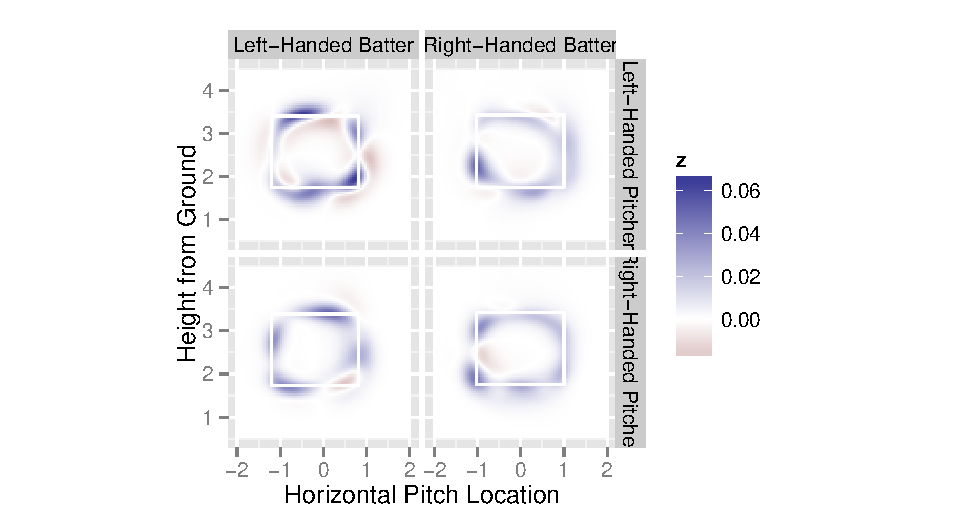
\includegraphics{images/prob-diff.pdf}
\caption{\label{fig:diff-probs}Difference between home and away pitchers in
the probability of a strike (provided the umpire has to make a
decision). The blue regions indicate a higher probability of a strike
for home pitchers and red regions indicate a higher probability of a
strike for away pitchers. Plots are faceted by the handedness of both
the pitcher and the batter.}
\end{figure}

The four different plots in Figure \ref{fig:diff-probs} represent the
four different combination of values among \texttt{p\_throws} and
\texttt{stand}. In general, provided that a pitcher throws to a batter
in the blue region, the pitch is more likely to be called a strike if
the pitcher is on their home turf. Interestingly, there is a
well-defined blue elliptical band around the boundaries of the typical
strike-zone. Thus, home pitchers are more likely to receive a favorable
call -- especially when the classification of the pitch is in question.
In some areas, the home pitcher has up to a 6 percent higher probability
of receiving a called strike than an away pitcher. The subtle
differences in spatial patterns across the different values of
\texttt{p\_throws} and \texttt{stand} are interesting as well. For
instance, pitching at home has a large positive impact for a left-handed
pitcher throwing in the lower inside portion of the strike-zone to a
right-handed batter, but the impact seems negligible in the mirror
opposite case. Differenced probabilistic densities are clearly an
interesting visual tool for analyzing PITCHf/x data. With
\texttt{strikeFX}, one can quickly and easily make all sorts of visual
comparisons for various situations. In fact, one can explore and compare
the probabilistic structure of any well-defined event over a strike-zone
region (for example, the probability a batter reaches base) using a
similar approach.

\subsection{2D animation}\label{d-animation}

\texttt{animateFX} provides convenient and flexible functionality for
animating the trajectory of any desired set of pitches. For
demonstration purposes, this section animates every four-seam and cut
fastball thrown by Mariano Rivera and Phil Hughes during the 2011
season. These pitches provide a good example of how facets play an
important role in extracting new insights. Similar methods can be used
to analyze any MLB player (or combination of players) in greater detail.

\texttt{animateFX} tracks three dimensional pitch locations over a
sequence of two dimensional plots. The animation takes on the viewpoint
of the umpire; that is, each time the plot refreshes, the balls are
getting closer to the viewer. This is reflected with the increase in
size of the points as the animation progresses. Obviously, some pitches
travel faster than others, which explains the different sizes within a
particular frame. Animations revert to the initial point of release once
\emph{all} of the baseballs have reached home plate. During an
interactive session, \texttt{animateFX} produces a series of plots that
may not viewed easily. One option available to the user is to wrap
\texttt{animation::saveHTML} around \texttt{animateFX} to view the
animation in a browser with proper looping controls (Xie
\protect\hyperlink{ref-animation}{2013}\protect\hyperlink{ref-animation}{a}).

To reduce the time and thinking required to produce these animations,
\texttt{animateFX} has default settings for the geometry, color, opacity
and size associated with each plot. Any of these assumptions can be
altered - except for the point geometry. In order for animations to
work, a data frame with the appropriately named PITCHf/x parameters
(that is, x0, y0, z0, vx0, vy0, vz0, ax0, ay0 and az0) is required. In
Figure \ref{fig:animate1}, every four-seam and cut fastball thrown by
Rivera and Hughes during the 2011 season is visualized using the
\texttt{pitches} data frame obtained earlier (the animation is available
at \url{http://cpsievert.github.io/pitchRx/ani1}).

\begin{Shaded}
\begin{Highlighting}[]
\KeywordTok{animateFX}\NormalTok{(pitches, }\DataTypeTok{layer=}\KeywordTok{list}\NormalTok{(}\KeywordTok{theme_bw}\NormalTok{(), }\KeywordTok{coord_equal}\NormalTok{(),}
  \KeywordTok{facet_grid}\NormalTok{(pitcher_name~stand, }\DataTypeTok{labeller =} \NormalTok{relabel)))}
\end{Highlighting}
\end{Shaded}

\begin{figure}
\centering
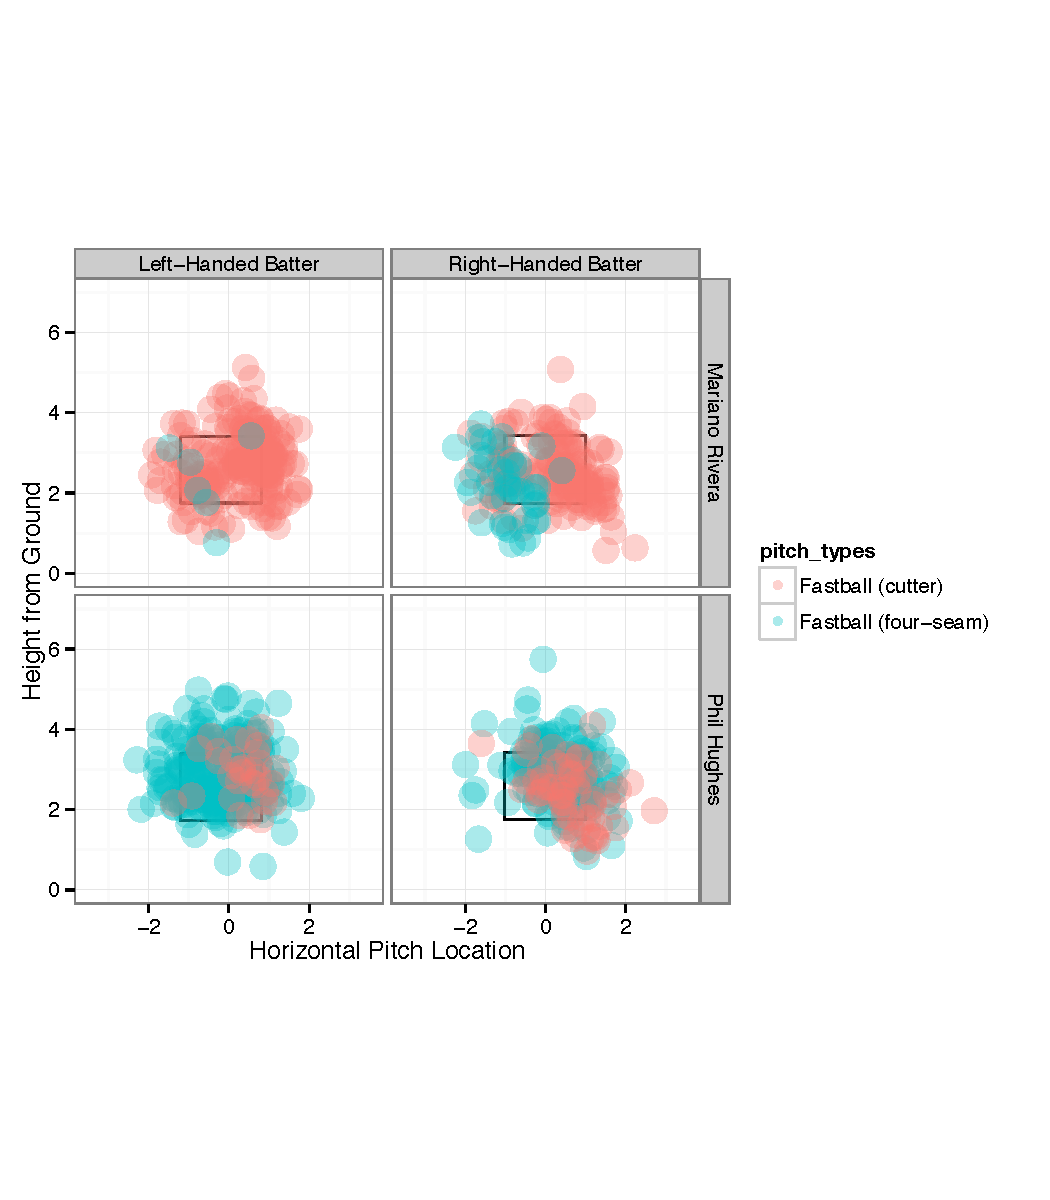
\includegraphics{images/ani-frame1.pdf}
\caption{\label{fig:animate1}The last frame of an animation of every
four-seam and cutting fastballs thrown by NY Yankee pitchers Mariano
Rivera and Phil Hughes during the 2011 season. The actual animation can
be viewed at \url{http://cpsievert.github.io/pitchRx/ani1}. Pitches are
faceted by pitcher and batting stance. For instance, the top left plot
portrays pitches thrown by Rivera to left-handed batters.}
\end{figure}

In the animation corresponding to Figure \ref{fig:animate1}, the upper
right-hand portion (Rivera throwing to right-handed batters) reveals the
clearest pattern in flight trajectories. Around the point of release,
Rivera's two pitch types are hard to distinguish. However, after a
certain point, there is a very different flight path among the two pitch
types. Specifically, the drastic left-to-right movement of the cut
fastball is noticeably different from the slight right-to-left movement
of the four-seam fastball. In recent years, cut fastballs have gained
notoriety among the baseball community as a coveted pitch for pitchers
have at their disposal. This is largely due to the difficulty that a
batter has in distinguishing the cut fastball from another fastball as
the ball travels toward home plate. Clearly, this presents an advantage
for the pitcher since they can use deception to reduce batter's ability
to predict where the ball will cross home plate. This deception factor
combined with Rivera's ability to locate his pitches explain his
accolades as one of the greatest pitchers of all time (Traub
\protect\hyperlink{ref-NYT}{2010}).

Although we see a clear pattern in Rivera's pitches, MLB pitchers are
hardly ever that predictable. Animating that many pitches for another
pitcher can produce a very cluttered graphic which is hard to interpret
(especially when many pitch types are considered). However, we may still
want to obtain an indication of pitch trajectory over a set of many
pitches. A way to achieve this is to average over the PITCHf/x
parameters to produce an overall sense of pitch type behavior (via the
\texttt{avg.by} option). Note that the facet variables are automatically
considered indexing variables. That is, in Figure \ref{fig:animate2},
there are eight `average' pitches since there are two pitch types, two
pitchers, and two types of batting stance (the animation is available at
\url{http://cpsievert.github.io/pitchRx/ani2}).

\begin{Shaded}
\begin{Highlighting}[]
\KeywordTok{animateFX}\NormalTok{(pitches, }\DataTypeTok{avg.by =} \StringTok{"pitch_types"}\NormalTok{, }\DataTypeTok{layer =} \KeywordTok{list}\NormalTok{(}\KeywordTok{coord_equal}\NormalTok{(), }\KeywordTok{theme_bw}\NormalTok{(),}
  \KeywordTok{facet_grid}\NormalTok{(pitcher_name~stand, }\DataTypeTok{labeller =} \NormalTok{relabel)))}
\end{Highlighting}
\end{Shaded}

\begin{figure}
\centering
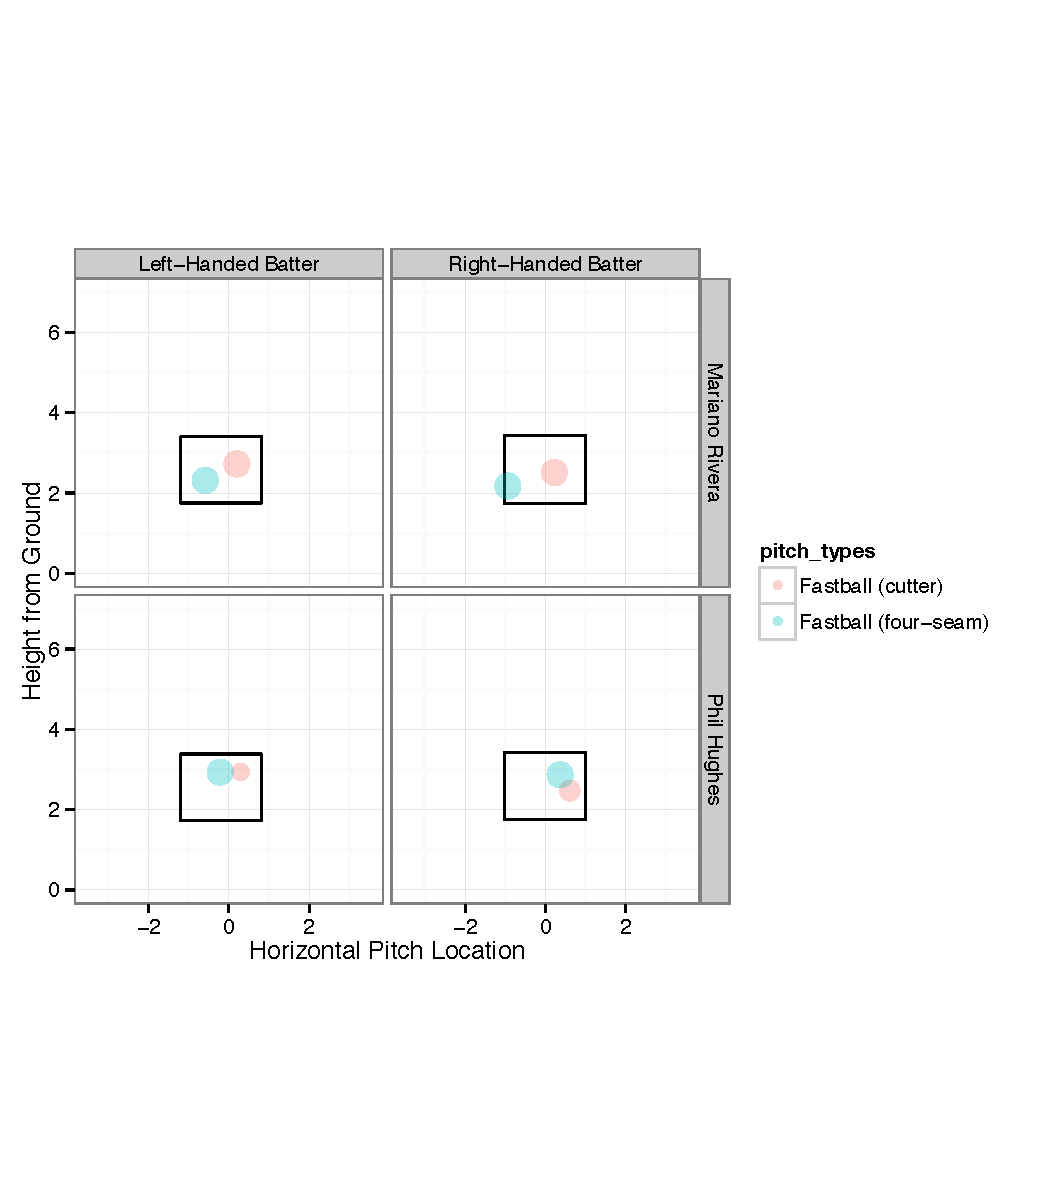
\includegraphics{images/ani-frame2.pdf}
\caption{\label{fig:animate2}The last frame of an animation of averaged
four-seam and cutting fastballs thrown by NY Yankee pitchers Mariano
Rivera and Phil Hughes during the 2011 season. The actual animation can
be viewed at \url{http://cpsievert.github.io/pitchRx/ani2}. PITCHf/x
parameters are averaged over pitch type, pitcher and batting stance. For
instance, the bottom right plot portrays an average four-seam and
average cutter thrown by Hughes to right-handed batters.}
\end{figure}

\subsection{Interactive 3D graphics}\label{interactive-3d-graphics}

\textbf{rgl} is an R package that utilizes OpenGL for graphics
rendering. \texttt{interactiveFX} utilizes \textbf{rgl} functionality to
reproduce flight paths on an interactive 3D platform. Figure
\ref{fig:rgl} has two static pictures of Mariano Rivera's 2011 fastballs
on this interactive platform. This is great for gaining new perspectives
on a certain set of pitches, since the trajectories can be viewed from
any angle. Figure \ref{fig:rgl} showcases the difference in trajectory
between Rivera's pitch types.

\begin{Shaded}
\begin{Highlighting}[]
\NormalTok{Rivera <-}\StringTok{ }\KeywordTok{subset}\NormalTok{(pitches, pitcher_name ==}\StringTok{ "Mariano Rivera"}\NormalTok{)}
\KeywordTok{interactiveFX}\NormalTok{(Rivera, }\DataTypeTok{avg.by =} \StringTok{"pitch_types"}\NormalTok{)}
\end{Highlighting}
\end{Shaded}

\begin{figure}
\centering
\includegraphics{images/rgl}
\caption{\label{fig:rgl}3D scatterplot of pitches from Rivera. Pitches are
plotted every one-hundredth of a second. Cutting fastballs are shown in
red and four-seam fastballs are shown in blue. The left hand plot takes
a viewpoint of Rivera and the right hand plot takes a viewpoint near the
umpire. Note these are static pictures of an interactive object.}
\end{figure}

\section{Conclusion}\label{conclusion}

\textbf{pitchRx} utilizes \textbf{XML2R}'s convenient framework for
manipulating XML content in order to provide easy access to PITCHf/x and
related Gameday data. \textbf{pitchRx} removes access barriers which
allows the average R user and baseball fan to spend their valuable time
analyzing Gameday's enormous source of baseball information.
\textbf{pitchRx} also provides a suite of functions that greatly reduce
the amount of work involved to create popular PITCHf/x graphics. For
those interested in obtaining other XML data, \textbf{pitchRx} serves as
a nice example of leveraging \textbf{XML2R} to quickly assemble custom
XML data collection mechanisms.

\chapter{LDAvis: A method for visualizing and interpreting topics}

This chapter is a paper published in The Proceedings of the Workshop on
Interactive Language Learning, Visualization, and Interfaces (ACL 2014)
(Sievert and Shirley \protect\hyperlink{ref-Sievert:2014b}{2014}). I am
the primary author of the paper which is avaliable online here
\url{http://nlp.stanford.edu/events/illvi2014/papers/sievert-illvi2014.pdf}

The formatting of paper has been modified to make for consistent
typesetting across the thesis.

\specialchapt{ABSTRACT}

We present \texttt{LDAvis}, an \texttt{R} package for creating We
present \texttt{LDAvis}, a web-based interactive visualization of topics
estimated using Latent Dirichlet Allocation that is built using a
combination of R and d3. Our visualization provides a global view of the
topics (and how they differ from each other), while at the same time
allowing for a deep inspection of the tokens most highly associated with
each individual topic. First, we propose a novel method for choosing
which tokens to present to a user to aid in the task of topic
interpretation, in which we define the \emph{relevance} of a token to a
topic. Second, we present the results of a user study that illustrates
how ranking tokens by their relevance to a given topic relates to that
topic's interpretability, and we recommend a default method of computing
relevance to maximize topic interpretability. Last, we incorporate
relevance into \texttt{LDAvis} in a way that allows users to flexibly
explore topic-token relationships to better understand a fitted LDA
model.

\section{Introduction}\label{section:introduction}

Recently much attention has been paid to visualizing the output of topic
models fit using Latent Dirichlet Allocation (LDA) (Matthew J. Gardner
and Seppi \protect\hyperlink{ref-Gardner}{2010}); (Chaney and Blei
\protect\hyperlink{ref-Blei-2012}{2012}); (Jason Chuang and Heer 2012b);
(Brynjar Gretarsson and Smyth \protect\hyperlink{ref-Gretarsson}{2011}).
Such visualizations are challenging to create because of the high
dimensionality of the fitted model -- LDA is typically applied to
thousands of documents, which are modeled as mixtures of dozens of
topics, which themselves are modeled as distributions over thousands of
tokens (David M. Blei and Jordan
\protect\hyperlink{ref-Blei-2003}{2012}); (Griffiths and Steyvers
\protect\hyperlink{ref-Griffiths}{2004}). The most promising basic
technique for creating LDA visualizations that are both compact and
thorough is \emph{interactivity}.

We introduce an interactive visualization system that we call
\texttt{LDAvis} that attempts to answer a few basic questions about a
fitted topic model: (1) What is the meaning of each topic?, (2) How
prevalent is each topic?, and (3) How do the topics relate to each
other? Different visual components answer each of these questions, some
of which are original, and some of which are borrowed from existing
tools.

Our visualization (illustrated in Figure \ref{fig:overview}) has two
basic pieces. First, the left panel of our visualization presents a
``global'' view of the topic model, and answers questions 2 and 3. In
this view, we plot the topics as circles in the two-dimensional plane
whose centers are determined by computing the distance between topics
(using a distance measure of the user's choice) and then by using
multidimensional scaling to project the inter-topic distances onto two
dimensions, as is done in (Jason Chuang and Heer 2012a). We encode each
topic's overall prevalence using the areas of the circles, where we sort
the topics in decreasing order of prevalence.

Second, the right panel of our visualization depicts a horizontal
barchart whose bars represent the individual tokens that are the most
useful for interpreting the currently selected topic on the left, and
allows users to answer question 1, ``What is the meaning of each
topic?''. A pair of overlaid bars represent both the corpus-wide
frequency of a given token as well as the topic-specific frequency of
the token, as in (Jason Chuang and Heer 2012b).

The left and right panels of our visualization are linked such that
selecting a topic (on the left) reveals the most useful tokens (on the
right) for interpreting the selected topic. In addition, selecting a
token (on the right) reveals the conditional distribution over topics
(on the left) for the selected token. This kind of linked selection
allows users to examine a large number of topic-token relationships in a
compact manner.

\begin{figure}
\centering
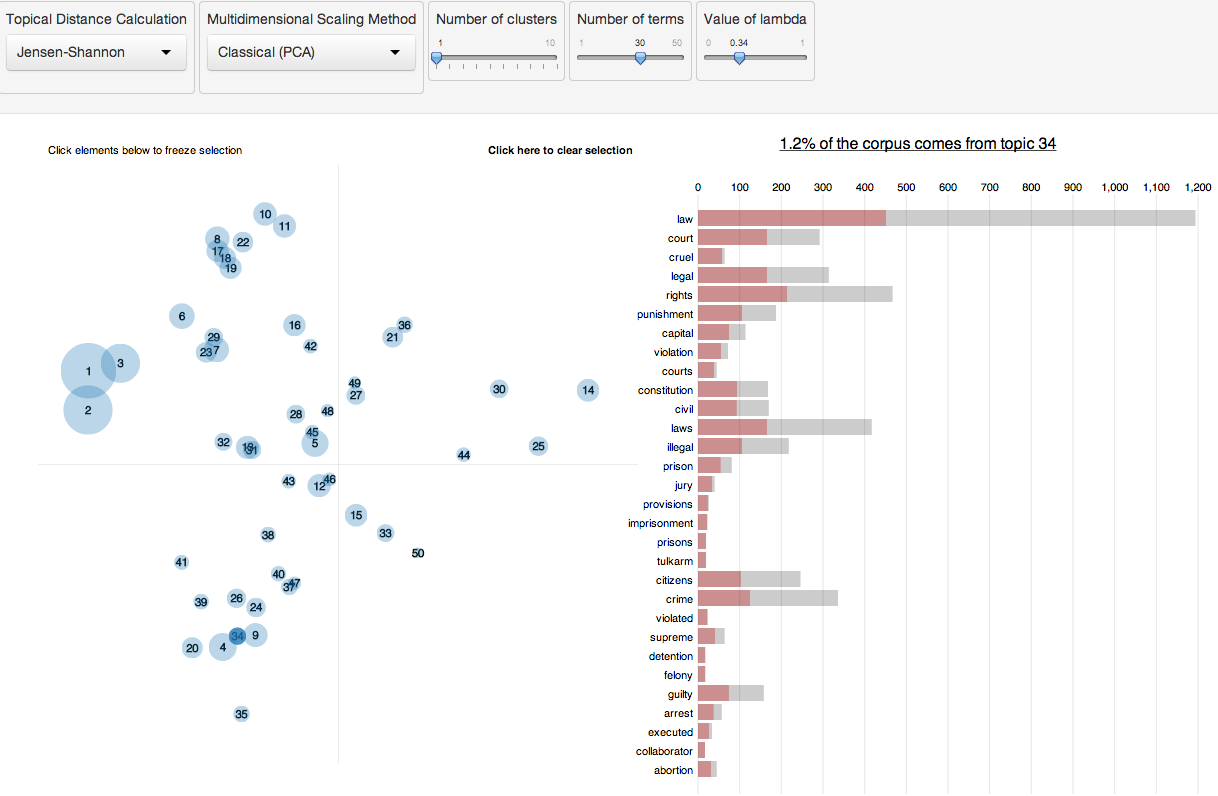
\includegraphics{images/fig_topic34b}
\caption{\label{fig:overview}The layout of LDAvis, with the global topic
view on the left, and the token barcharts on the right. Linked
selections allow users to reveal aspects of the topic-token
relationships compactly.}
\end{figure}

A key innovation of our system is how we determine the most useful
tokens for interpreting a given topic, and how we allow users to
interactively adjust this determination. A topic in LDA is a multinomial
distribution over the tokens in the vocabulary, where the vocabulary
typically contains thousands of tokens. To interpret a topic, one
typically examines a ranked list of the most probable tokens in that
topic, using anywhere from three to thirty tokens in the list. The
problem with interpreting topics this way is that common tokens in the
corpus often appear near the top of such lists for multiple topics,
making it hard to differentiate the meanings of these topics.

Bischof and Airoldi (\protect\hyperlink{ref-Bischof}{2012}) propose
ranking tokens for a given topic in terms of both the \emph{frequency}
of the token under that topic as well as the token's \emph{exclusivity}
to the topic, which accounts for the degree to which it appears in that
particular topic to the exclusion of others. We propose a similar
measure that we call the \emph{relevance} of a token to a topic to
create a flexible method for ranking tokens in order of usefulness for
interpreting topics. We discuss our definition of relevance, and its
graphical interpretation, in detail in Section \ref{section:relevance}.
We also present the results of a user study conducted to determine the
optimal tuning parameter in the definition of relevance to aid the task
of topic interpretation in
Section\textasciitilde{}\ref{section:userstudy}, and we describe how we
incorporate relevance into our interactive visualization in
Section\textasciitilde{}\ref{section:system}.

\section{Related Work}\label{section:relatedwork}

Much work has been done recently regarding the interpretation of topics
(i.e.~measuring topic ``coherence'') as well as visualization of topic
models.

\subsection{Topic Interpretation and Coherence}

It is well-known that the topics inferred by LDA are not always easily
interpretable by humans. Jonathan Chang and Blei
(\protect\hyperlink{ref-Chang}{2009}) established via a large user study
that standard quantitative measures of fit, such as those summarized by
Hanna M. Wallach and Mimno (\protect\hyperlink{ref-Wallach}{2009}), do
not necessarily agree with measures of topic interpretability by humans.
Daniel Ramage et al. (\protect\hyperlink{ref-Ramage}{2009}) assert that
``characterizing topics is hard'' and describe how using the top-\(k\)
tokens for a given topic might not always be best, but offer few
concrete alternatives.

Loulwah AlSumait and Domeniconi
(\protect\hyperlink{ref-AlSumait}{2009}), David Mimno and McCallum
(\protect\hyperlink{ref-Mimno}{2011}), and Jason Chuang and Heer (2013b)
develop quantitative methods for measuring the interpretability of
topics based on experiments with data sets that come with some notion of
topical ground truth, such as document metadata or expert-created topic
labels. These methods are useful for understanding, in a global sense,
which topics are interpretable (and why), but they don't specifically
attempt to aid the user in interpreting \emph{individual} topics.

Blei and Lafferty (\protect\hyperlink{ref-Blei-2009}{2009}) developed
``Turbo Topics'', a method of identifying n-grams within LDA-inferred
topics that, when listed in decreasing order of probability, provide
users with extra information about the usage of tokens within topics.
This two-stage process yields good results on experimental data,
although the resulting output is still simply a ranked list containing a
mixture of tokens and n-grams, and the usefulness of the method for
topic interpretation was not tested in a user study.

David Newman and Baldwin (\protect\hyperlink{ref-Newman-JCDL}{2010})
describe a method for ranking tokens within topics to aid
interpretability called Pointwise Mutual Information (PMI) ranking.
Under PMI ranking of tokens, each of the ten most probable tokens within
a topic are ranked in decreasing order of approximately how often they
occur in close proximity to the nine other most probable tokens from
that topic in some large, external ``reference'' corpus, such as
Wikipedia or Google n-grams. Although this method correlated highly with
human judgments of token importance within topics, it does not easily
generalize to topic models fit to corpora that don't have a readily
available external source of word co-occurrences.

In contrast, Taddy (\protect\hyperlink{ref-Taddy}{2011}) uses an
intrinsic measure to rank tokens within topics: a quantity called
\emph{lift}, defined as the ratio of a token's probability within a
topic to its marginal probability across the corpus. This generally
decreases the rankings of globally frequent tokens, which can be
helpful. We find that it can be noisy, however, by giving high rankings
to very rare tokens that occur in only a single topic, for instance.
While such tokens may contain useful topical content, if they are very
rare the topic may remain difficult to interpret.

Finally, Bischof and Airoldi (\protect\hyperlink{ref-Bischof}{2012})
propose and implement a new statistical topic model that infers both a
token's frequency as well as its \emph{exclusivity} -- the degree to
which its occurrences are limited to only a few topics. They introduce a
univariate measure called a FREX score (``\(\mathbf{FR}\)equency and
\(\mathbf{EX}\)clusivity'') which is a weighted harmonic mean of a
token's rank within a given topic with respect to frequency and
exclusivity, and they recommend it as a way to rank tokens to aid topic
interpretation. We propose a similar method that is a weighted average
of a token's probability and its lift, and we justify it with a user
study and incorporate it into our interactive visualization.

\subsection{Topic Model Visualization Systems}

A number of visualization systems for topic models have arisen in recent
years. Several of them focus on allowing users to browse documents,
topics, and tokens to learn about the relationships between these three
canonical topic model units (Matthew J. Gardner and Seppi
\protect\hyperlink{ref-Gardner}{2010}); (Chaney and Blei
\protect\hyperlink{ref-Blei-2012}{2012}) (Justin Snyder and Wolfe
\protect\hyperlink{ref-Snyder}{2013}). These browsers typically use
lists of the most probable tokens within topics to summarize the topics,
and the visualization elements are limited to barcharts or word clouds
of token probabilities for each topic, pie charts of topic probabilities
for each document, and/or various barcharts or scatterplots related to
document metadata. Although these tools can be useful for browsing a
corpus, we seek a more compact visualization, with the more narrow focus
of quickly and easily understanding the individual topics themselves
(without necessarily visualizing documents).

Jason Chuang and Heer (2012b) develop such a tool, called ``Termite'',
which visualizes the set of topic-token distributions estimated in LDA
using a matrix layout. The authors introduce two measures of the
usefulness of tokens for understanding a topic model:
\emph{distinctiveness} and \emph{saliency}. These quantities measure how
much information a token conveys about a topic by computing the
Kullback-Liebler divergence between the distribution of topics given the
token and the marginal distribution of topics (distinctiveness),
optionally weighted by the token's overall frequency (saliency). The
authors recommend saliency as a thresholding method for selecting which
tokens are included in the visualization, and they further use a
seriation method for ordering the most salient tokens to highlight
differences between topics.

Termite is a compact, intuitive interactive visualization of the topics
in a topic model, but by only including tokens that rank high in
saliency or distinctiveness, which are \emph{global} properties of
tokens, it is restricted to providing a \emph{global} view of the model,
rather than allowing a user to deeply inspect individual topics by
visualizing a potentially different set of tokens for every single
topic. In fact, Jason Chuang and Heer (2013a) describe the use of a
``topic-specific word ordering'' as potentially useful future work.

\section{Relevance of tokens to topics}

Here we define \emph{relevance}, our method for ranking tokens within
topics, and we describe the results of a user study to learn an optimal
tuning parameter in the computation of relevance.

\subsection{Definition of Relevance}\label{section:relevance}

Let \(\phi_{kw}\) denote the probability of token
\(w \in \{1, ..., V\}\) for topic \(k\in \{1, ..., K\}\), where \(V\)
denotes the number of unique tokens in the vocabulary, and let \(p_w\)
denote the marginal probability of token \(w\) in the corpus. One
typically estimates \(\phi\) in LDA using Variational Bayes methods or
Collapsed Gibbs Sampling, and \(p_w\) from the empirical distribution of
the corpus (optionally smoothed by including prior weights as
pseudo-counts).

We define the \emph{relevance} of token \(w\) to topic \(k\) given a
weight parameter \(\lambda\) (where \(0 \leq \lambda \leq 1\)) as: \[
r(w, k \mid \lambda) = \lambda \log(\phi_{kw}) + (1 - \lambda)\log\Bigl(\frac{\phi_{kw}}{p_w}\Bigr),
\] where \(\lambda\) determines the weight given to the probability of
token \(w\) under topic \(k\) relative to its lift. Setting
\(\lambda = 1\) results in the familiar ranking of tokens in decreasing
order of their topic-specific probability, and setting \(\lambda = 0\)
ranks tokens solely by their lift, which we found anecdotally to result
in ``noisy'' topics full of rare tokens. We wish to learn an ``optimal''
value of \(\lambda\) for topic interpretation from our user study.

First, though, to see how different values of \(\lambda\) result in
different ranked token lists, consider the plot in Figure
\ref{fig:relevance}. We fit a 50-topic model to the 20 Newsgroups data
(details are described in
Section\textasciitilde{}\ref{section:userstudy}) and plotted
\(\log\)(lift) on the \(y\)-axis vs. \(\log(\phi_{kw})\) on the
\(x\)-axis for each token in the vocabulary (which has size
\(V=22,524\)) for a given topic. Figure \ref{fig:relevance} shows this
plot for Topic 29, which occurred mostly in documents posted to the
``Motorcycles'' newsgroup, but also from documents posted to the
``Automobiles'' newsgroup and the ``Electronics'' newsgroup.
Graphically, the line separating the most relevant tokens for this
topic, given \(\lambda\), has slope \(-\lambda/(1 - \lambda)\) (see
Figure \ref{fig:relevance}).

For this topic, the top-5 most relevant tokens given \(\lambda = 1\)
(ranking solely by probability) are \{out, \#emailaddress,
\#twodigitnumer, up, \#onedigitnumber\}, where a `\#' symbol denotes a
token that is an entity representing a class of things. In contrast to
this list, which contains globally common tokens and which provides very
little meaning regarding motorcycles, automobiles, or electronics, the
top-5 most relevant tokens given \(\lambda = 1/3\) are \{oil, plastic,
pipes, fluid, and lights\}. The second set of tokens is much more
descriptive of the topic being discussed than the first.

\begin{figure}
\centering
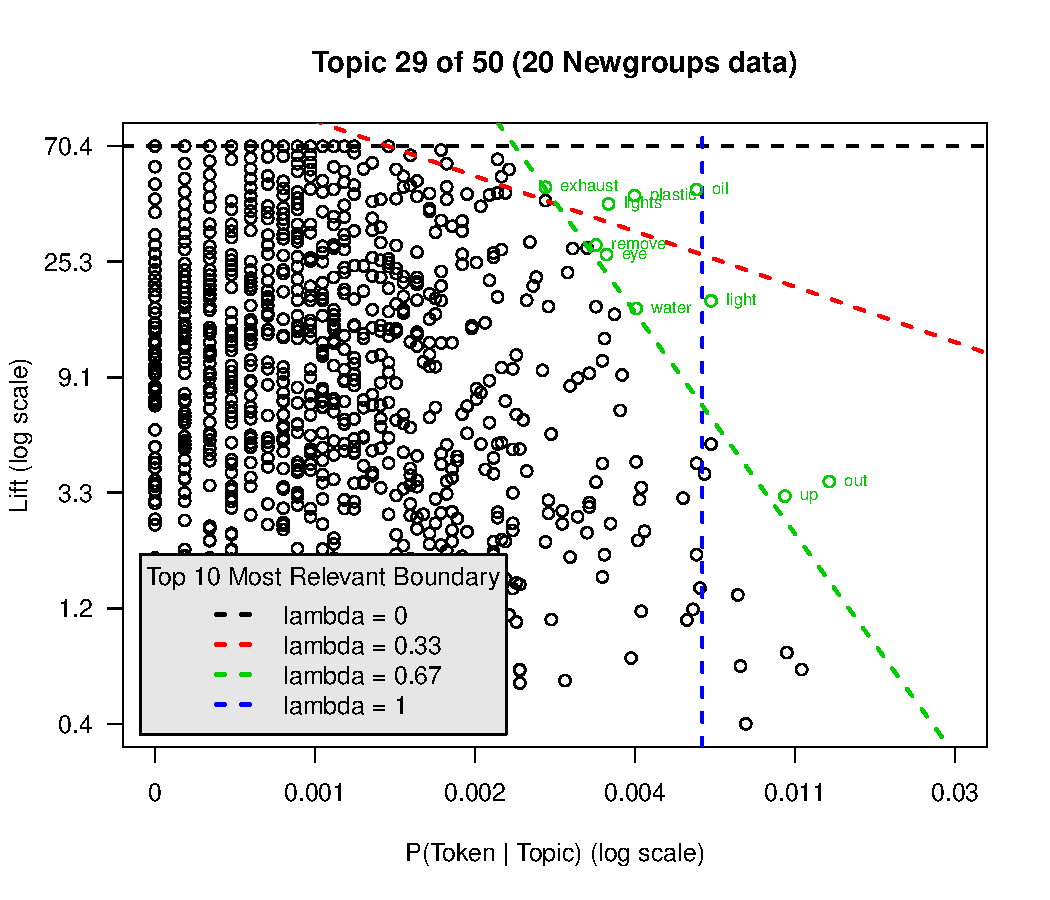
\includegraphics{images/fig_topic29.pdf}
\caption{\label{fig:relevance}Dotted lines separating the top-10 most
relevant tokens for different values of \(\lambda\), with the most
relevant tokens for \(\lambda\) = 2/3 displayed and highlighted in
green.}
\end{figure}

\subsection{User Study}\label{section:userstudy}

We conducted a user study to determine whether there was an optimal
value of \(\lambda\) in the definition of relevance to aid topic
interpretation. First, we fit a 50-topic model to the \(D=13,695\)
documents in the 20 Newsgroups data which were posted to a single
Newsgroup (rather than two or more Newsgroups). We used the Collapsed
Gibbs Sampler algorithm (Griffiths and Steyvers
\protect\hyperlink{ref-Griffiths}{2004}) to sample the latent topics for
each of the \(N=1,590,376\) tokens in the data, and we saved their topic
assignments from the last iteration (after convergence). We then
computed the 20 by 50 table, \(T\), which contains, in cell \(T_{gk}\),
the count of the number of times a token from topic
\(k \in \{1, ..., 50\}\) was assigned to Newsgroup
\(g \in \{1, ..., 20\}\), where we defined the Newsgroup of a token to
be the Newsgroup to which the document containing that token was posted.
Some of the LDA-inferred topics occurred almost exclusively (\(>90\)\%
of occurrences) in documents from a single Newsgroup, such as Topic 38,
which was the estimated topic for 15,705 tokens in the corpus, 14,233 of
which came from documents posted to the ``Medicine'' (or ``sci.med'')
Newsgroup. Other topics occurred in a wide variety of Newsgroups. One
would expect these ``spread-out'' topics to be harder to interpret than
the ``pure'' topics like Topic 38.

In the study we recruited 29 subjects among our colleagues, and each
subject completed an online experiment consisting of 50 tasks, one for
each topic in the fitted LDA model. Task \(k\) (for
\(k \in \{1, ..., 50\}\)) was to read a list of five tokens, ranked from
1-5 in terms of relevance to topic \(k\), where \(\lambda \in (0, 1)\)
was randomly sampled to compute relevance. The user was instructed to
identify which ``topic'' the list of tokens discussed from a list of
three possible ``topics'', where their choices were names of the
Newsgroups. The correct answer for task \(k\) (i.e.~our ``ground
truth'') was defined as the Newsgroup that contributed the most tokens
to topic \(k\) (i.e.~the Newsgroup with the largest count in the \(k\)th
column of the table \(T\)), and the two alternative choices were the
Newsgroups that contributed the second and third-most tokens to topic
\(k\).

We anticipated that the effect of \(\lambda\) on the probability of a
user making the correct choice could be different across topics. In
particular, for ``spread-out'' topics that were inherently difficult to
interpret, because their tokens were drawn from a wide variety of
Newsgroups (similar to a ``fused'' topic in Jason Chuang and Heer
(2013b)), we expected the proportion of correct responses to be roughly
1/3 no matter the value of \(\lambda\) used to compute relevance.
Similarly, for very ``pure'' topics, whose tokens were drawn almost
exclusively from one Newsgroup, we expected the task to be easy for any
value of \(\lambda\). To account for this, we analyzed the experimental
data by fitting a varying-intercepts logistic regression model to allow
each of the fifty topics to have its own baseline difficulty level,
where the effect of \(\lambda\) is shared across topics. We used a
quadratic function of \(\lambda\) in the model (linear, cubic and
quartic functions were explored and rejected).

As expected, the baseline difficulty of each topic varied widely. In
fact, seven of the topics were correctly identified by all 29 users, and
one topic was incorrectly identified by all 29 users. For the remaining
42 topics we estimated a topic-specific intercept term to control for
the inherent difficulty of identifying the topic (not just due to its
tokens being spread among multiple Newsgroups, but also to account for
the inherent familiarity of each topic to our subject pool -- subjects,
on average, were more familiar with ``Cars'' than ``The X Window
System'', for example).

\begin{figure}
\centering
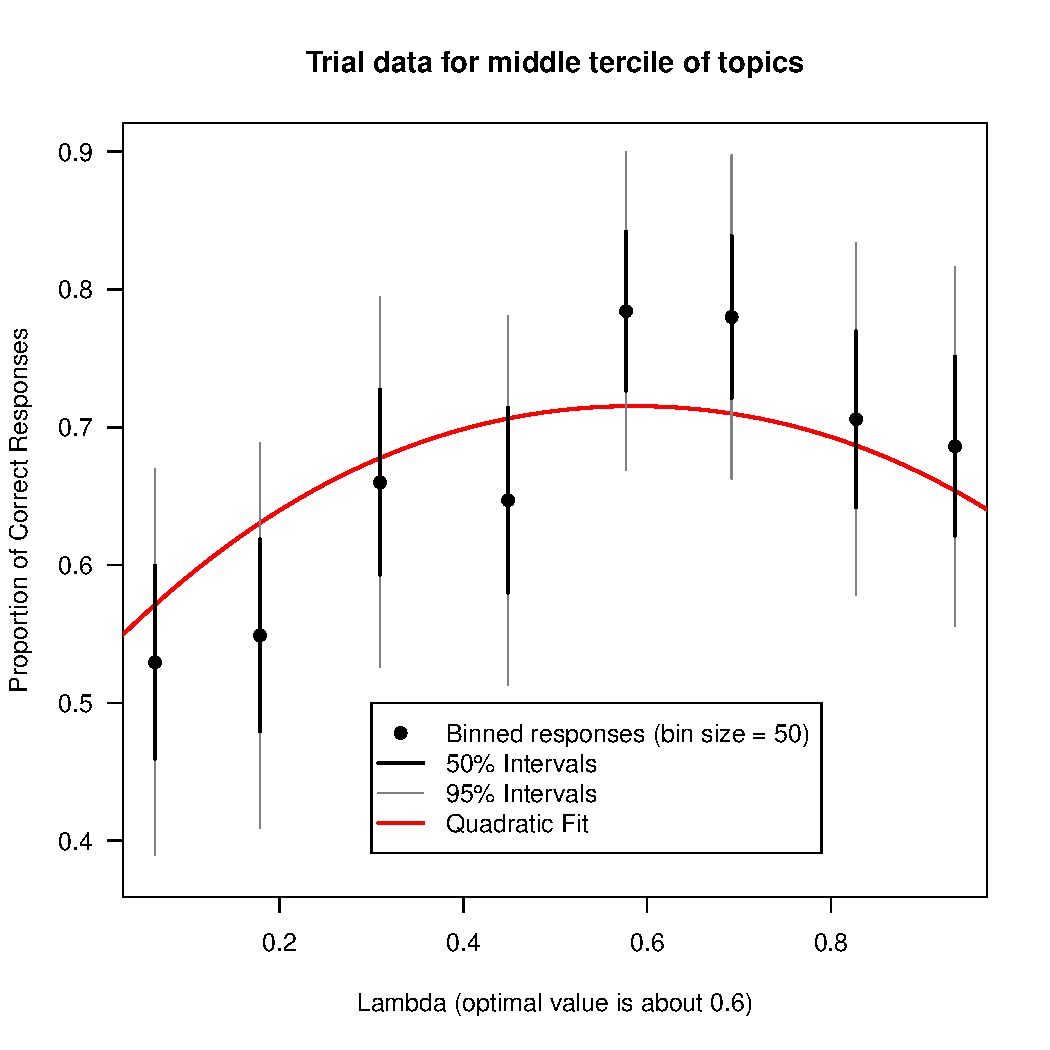
\includegraphics{images/fig_lambda.pdf}
\caption{\label{fig:lambda}A plot of the proportion of correct responses in
a user study vs.~the value of \(\lambda\) used to compute the most
relevant tokens for each topic.}
\end{figure}

The estimated effects of \(\lambda\) and \(\lambda^2\) were 2.74 and
-2.34, with standard errors 1.03 and 1.00. Taken together, their joint
effect was statistically significant (\(\chi^2\) p-value = 0.018). \%,
but the signs of their coefficients agreed with out intuition, and in a
similarly designed large-scale user study (on Mechanical Turk, for
instance), we expect that their joint effect would be statistically
significant. To see the estimated effect of \(\lambda\) on the
probability of correctly identifying a topic, consider Figure
\ref{fig:lambda}. We plot binned proportions of correct responses (on
the y-axis) vs. \(\lambda\) (on the x-axis) for the 14 topics whose
estimated topic-specific intercepts fell into the middle tercile among
the 42 topics that weren't trivial or impossible to identify. Among
these topics there was roughly a 67\% baseline probability of correct
identification. As Figure \ref{fig:lambda} shows, for these topics, the
``optimal'' value of \(\lambda\) was about 0.6, and it resulted in a
70\% - 75\% probability of correct identification, whereas for values of
\(\lambda\) near 0 or 1, the proportion of correct responses was closer
to 55\% or 60\%. We view this as evidence that ranking tokens according
to relevance, where \(\lambda < 1\), can aid topic interpretation, even
if this precise task (selecting a known topic label from a list of
pre-defined labels associated with each document as metadata) is not
always the goal. A similar conclusion might be drawn from an experiment
to study the FREX token ranking method of Bischof and Airoldi
(\protect\hyperlink{ref-Bischof}{2012}).

Note that in our experiment, we used the collection of single-posted 20
Newsgroups documents to define our ``ground truth'' data. An alternative
method for collecting ``ground truth'' data would have been to recruit
experts to label topics from an LDA model. We chose against this option
because doing so would present a classic ``chicken-or-egg'' problem: If
we use expert-labeled topics in an experiment to learn how to summarize
topics so that they can be interpreted (i.e. ``labeled''), we would only
re-learn the way that our experts were instructed, or allowed, to label
the topics in the first place! If, for instance, the experts were
presented with a ranked list of the most probable tokens for each topic,
this would influence the interpretations and labels they give to the
topics, and the experimental result would be the circular conclusion
that ranking tokens by probability allows users to recover the
``expert'' labels most easily. To avoid this, we felt strongly that we
should use data in which documents have metadata associated with them.
The 20 Newsgroups data provides an externally validated source of topic
labels, in the sense that the labels were presented to users (in the
form of Newsgroup names), and users subsequently filled in the content.
It represents, essentially, a crowd-sourced collection of tokens, or
content, for a certain set of topic labels.

\section{Our Visualization System}\label{section:system}

Our interactive, web-based visualization system, \texttt{LDAvis}, has
two core functionalities that enable users to understand the topic-token
relationships in a fitted LDA model, and a number of extra features that
provide additional perspectives on the model. \%Usually these questions
can not be answered easily with a few simple plots and/or metrics.
Instead, an interactive layout such as \texttt{LDAvis} allows one to
quickly explore model output, form new hypotheses and verify findings.

\begin{figure}
\centering
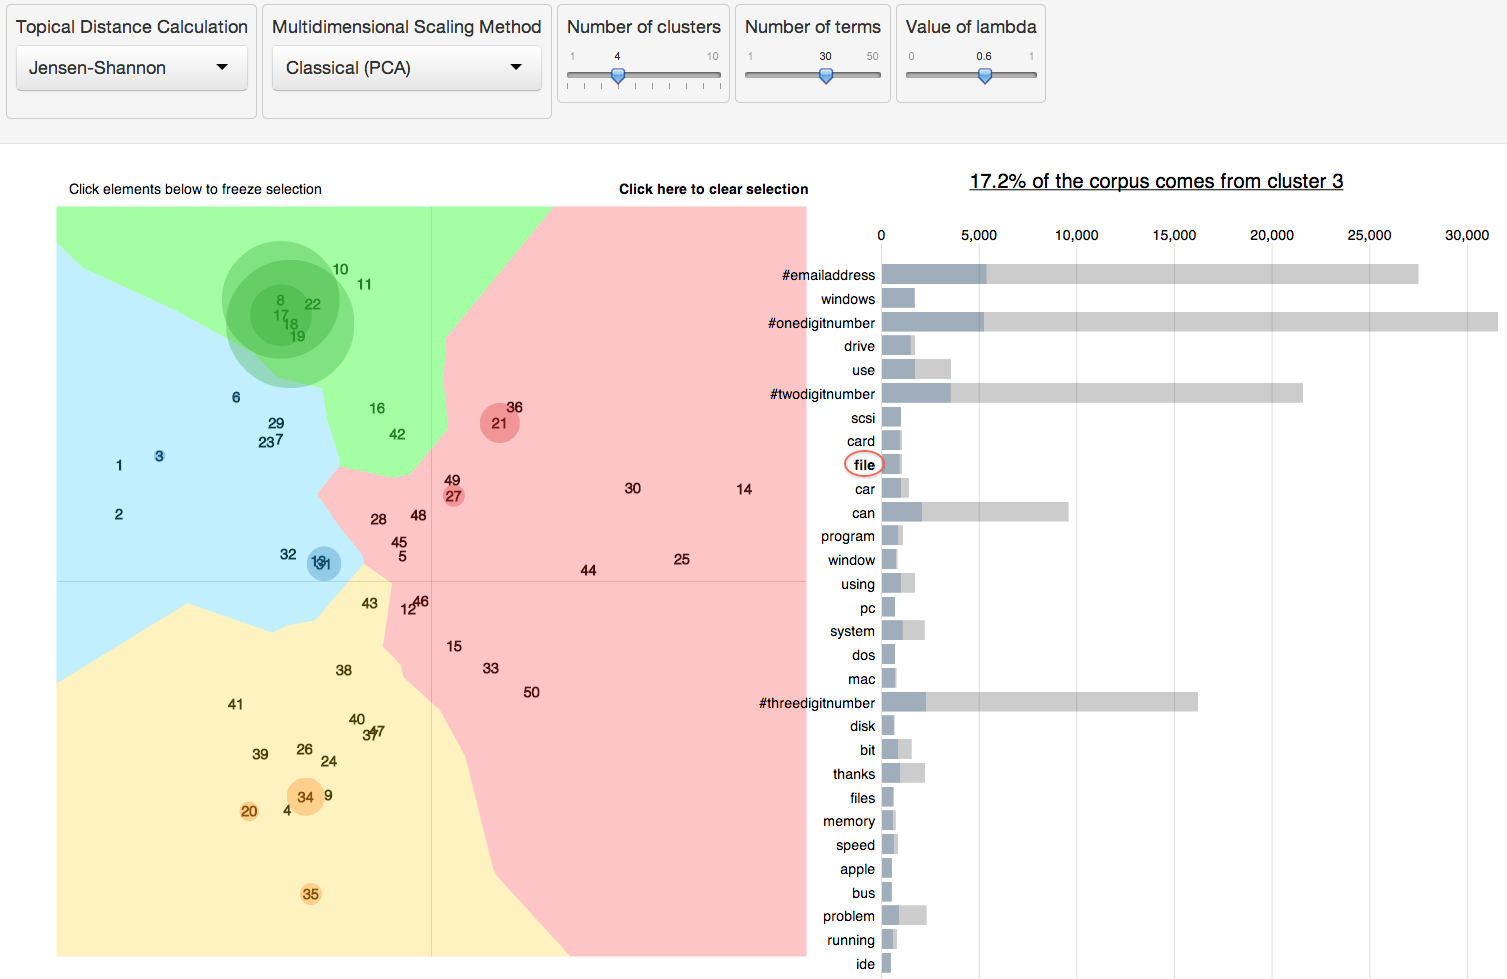
\includegraphics{images/fig_file_new2}
\caption{\label{fig:file}The user has chosen to segment the topics into four
clusters, and has selected the green cluster to populate the barchart
with the most relevant tokens for that cluster. Then, the user hovered
over the ninth bar from the top, `file', to display the conditional
distribution over topics for this token.}
\end{figure}

First and foremost, \texttt{LDAvis} allows one to select a topic to
reveal the most relevant tokens for that topic. In Figure
\ref{fig:overview}, Topic 34 is selected, and its 30 most relevant
tokens (given \(\lambda\) = 0.34, in this case) populate the bar chart
to the right (ranked in order of relevance from top to bottom). The
widths of the gray bars represent the corpus-wide frequencies of each
token, and the widths of the red bars represent the topic-specific
frequencies of each token. A slider allows users to change the value of
\(\lambda\), which can alter the rankings of tokens to aid topic
interpretation. By default, \(\lambda\) is set to 0.6, as suggested by
our user study in Section\textasciitilde{}\ref{section:userstudy}. If
\(\lambda = 1\), tokens are ranked solely by \(\phi_{kw}\), which
implies the red bars would be sorted from widest (at the top) to
narrowest (at the bottom). By comparing the widths of the red and gray
bars for a given token, users can quickly understand whether a token is
highly relevant to the selected topic because of its lift (a high ratio
of red to gray), or its probability (absolute width of red). The top 3
most relevant tokens in Figure \ref{fig:overview} are ``law'',
``rights'', and ``court''. Note that ``law'' is a common word which is
generated by Topic 34 in about 40\% of its corpus-wide occurrences,
whereas ``cruel'' is a relatively rare word with very high lift -- it
occurs almost exclusively in Topic 34. Such properties of the
topic-token relationship are readily visible in \texttt{LDAvis} for
every topic.

On the left panel, two visual features provide a global perspective of
the topics. First, the areas of the circles are proportional to the
relative prevalences of the topics in the corpus, \(\theta_k\), which
can be computed as \(\theta_k = \sum_d N_d\theta_{dk}\) for documents
\(d = 1, ..., D\), where document \(d\) contains \(N_d\) tokens. In the
50-topic model fit to the 20 Newsgroups data, the first three topics
comprise 12\%, 9\%, and 6\% of the corpus, and all contain common,
non-specific tokens (although there are differences: Topic 2 contains
formal debate-related language such as ``conclusion'', ``evidence'', and
``argument'', whereas Topic 3 contains slang conversational language
such as ``kinda'', ``like'', and ``yeah''). In addition to visualizing
topic prevalence, the left pane shows inter-topic differences. The
default for computing inter-topic distances is Jensen-Shannon
divergence, although other metrics are enabled. The default for scaling
the set of inter-topic distances defaults to Principal Components, but
other other algorithms are also enabled.

The second core feature of \texttt{LDAvis} is the ability to select a
token (by hovering over it) to reveal its conditional distribution over
topics. This distribution is visualized by altering the areas of the
topic circles such that they are proportional to the token-specific
frequencies across the corpus. This allows the user to verify, as
discussed in Jason Chuang and Heer (2012a), whether the multidimensional
scaling of topics has faithfully clustered similar topics in
two-dimensional space. For example, in Figure \ref{fig:file}, the token
``file'' is selected. In the majority of this token's occurrences, it is
drawn from one of several topics located in the upper left-hand region
of the global topic view. Upon inspection, this group of topics can be
interpreted broadly as a discussion of computer hardware and software.
This verifies, to some extent, their placement, via multidimensional
scaling, into the same two-dimensional region. It also suggests that the
word ``file'' used in this context refers to a computer file. However,
there is also conditional probability mass for the token ``file'' on
Topic 34. As shown in Figure \ref{fig:overview}, Topic 34 can be
interpreted as discussing the criminal punishment system where ``file''
refers to court filings. Similar discoveries can be made for any word
that exhibits polysemy (such as ``drive'' appearing in computer- and
automobile-related topics, or ``ground'' occurring in electrical- and
baseball-related topics).

Beyond its within-browser interaction capability, \texttt{LDAvis}
leverages the \texttt{R} language to allow users to easily alter the
topical distance measurement as well as the multidimensional scaling
algorithm to produce the global topic view. In addition, there is an
option to apply \(k\)-means clustering to the topics (as a function of
their two-dimensional locations in the global topic view). This is
merely an effort to facilitate semantic zooming in an LDA model with
many topics where `after-the-fact' clustering may be an easier way to
learn clusters of topics, rather than fitting a hierarchical topic model
(David M. Blei and Tenenbaum
\protect\hyperlink{ref-Blei-hierarchical}{2003}), for example. Selecting
a cluster (or region) of topics reveals the most relevant tokens for
that group of topics, where the token distribution of a cluster of
topics is defined as the average of the token distributions of the
individual topics in the cluster. In Figure \ref{fig:file}, the green
cluster of topics is selected, and the most relevant tokens are
predominantly related to computer hardware and software.

\section{Discussion}\label{section:futurework}

We have described a web-based, interactive visualization system,
\texttt{LDAvis}, that enables deep inspection of topic-token
relationships in an LDA model, while simultaneously providing a
``global'' view of the topics, via their prevalences and similarities to
each other, in a compact space. We also propose a novel way to rank
tokens within topics to aid in the task of topic interpretation, and we
present a user study that attempts to not only \emph{measure} the
interpretability of a topic, but also how to \emph{maximize} the
interpretability of the topic.

For future work, we anticipate performing a larger user study to further
understand how to facilitate topic interpretation in fitted LDA models,
including a comparison of multiple methods, such as ranking by Turbo
Topics (Blei and Lafferty \protect\hyperlink{ref-Blei-2009}{2009}) or
FREX scores (Bischof and Airoldi \protect\hyperlink{ref-Bischof}{2012}),
in addition to relevance. We also note the need to visualize
correlations between topics, as this can provide insight into what is
happening on the document level without actually displaying entire
documents. Last, we seek a solution to the problem of visualizing a
large number of topics (say, from 100 - 500 topics) in a compact way.

\chapter{Extending ggplot2's grammar of graphics implementation for linked and dynamic graphics on the web} \label{sec:animint}

This chapter is a paper currently under revision with intention of
submitting to the Journal of Computational and Graphical Statistics. I
am the primary author of the paper and there is a working draft
available here --
\url{https://github.com/tdhock/animint-paper/blob/jcgs/HOCKING-animint.pdf}

The formatting of paper has been modified to make for consistent
typesetting across the thesis.

\specialchapt{ABSTRACT}

The web is the most popular medium for sharing interactive data
visualizations thanks to the portability of the web browser and the
accessibility of the internet. Unfortunately, creating interactive web
graphics often requires a working knowledge of numerous web technologies
that are foreign to many people working with data. As a result, web
graphics are rarely used for exploratory data analysis where quick
iteration between different visualizations is of utmost importance. This
is the core strength of ggplot2, a popular data visualization package
for R, the world's leading open-source statistical programming language.
The conceptual framework behind ggplot2 is based on the grammar of
graphics, which lays a foundation for describing any static graphic as a
small set of independent components. Perhaps the most fundamental
component is the mapping from abstract data to the visual space,
sometimes referred to as the aesthetic mapping. We propose adding two
new aesthetics to the grammar, which together are sufficient for
elegantly describing both animations and certain classes of coordinated
linked views. We implement this extension in the open-source R package
animint, which converts ggplot2 objects to interactive web
visualizations via D3.

\section{Introduction}
\label{sec:intro}

The world's leading open source statistical programming language, R, has
a rich history of interfacing with computational tools for the use of
people doing data analysis and statistics research (R Core Team
\protect\hyperlink{ref-RCore}{2015}). Understanding R's core audience is
important, as they typically want to maximize their time working on data
analysis problems, and minimize time spent learning computational tools.
R excels in this regard, as it is designed specifically for interactive
use, where users can quickly explore their data using highly expressive
interfaces. Another key player in R's success story is its packaging
infrastructure, which provides tools for distributing entire research
conpendium(s) (code, data, documentation, auxiliary documents, etc)
(Gentleman and Lang \protect\hyperlink{ref-Gentleman:Lang}{2004}).

One of the most widely used R packages is ggplot2 (Wickham
\protect\hyperlink{ref-ggplot2-book}{2009}\protect\hyperlink{ref-ggplot2-book}{b}),
a data visualization package inspired by the grammar of graphics
(Wilkinson et al. \protect\hyperlink{ref-wilkinson}{2006}). In fact,
Donoho (\protect\hyperlink{ref-Donoho:2015tu}{2015}) writes: ``This
effort may have more impact on today's practice of data analysis than
many highly-regarded theoretical statistics papers``. In our experience,
ggplot2 has made an impact thanks to its foundation in the grammar of
graphics, carefully chosen defaults, and overall usability. This helps
data analysts rapidly iterate and discover informative visualizations --
an essential task in exploratory data analysis (EDA). When dealing with
high-dimensional data, however, it is often useful to produce
interactive and/or dynamic graphics, which ggplot2 does not inherently
support.

Interactive graphics toolkits in R have been used for decades to enhance
the EDA workflow, but these approaches are often not easy to reproduce
or distribute to a larger audience. It is true that most graphics
generated during EDA are ultimately not useful, but sometimes,
understanding gained during this phase is most easily shared via the
interactive graphics themselves. Thus, there is value is being able to
easily share, and embed interactive graphics inside a larger report.
Unfortunately, this is typically hard, if not impossible, using
traditional interactive graphics toolkits. As a result, there is a large
disconnect between the visualization tools that we use for exploration
versus presentation.

We aim to narrow this gap in visualization tools by extending ggplot2's
grammar of graphics implementation for interactive and dynamic web
graphics. Our extension allows one to create animated transitions and
perform database queries via direct manipulation of linked views like
those described in (Ahlberg, Williamson, and Shneiderman
\protect\hyperlink{ref-Ahlberg:1991}{1991}) and (Buja et al.
\protect\hyperlink{ref-Buja:1991vh}{1991}). A conceptual model for our
extension is provided in Section \ref{sec:extension} and Section
\ref{sec:animation}. In Section \ref{sec:worldbank}, we demonstrate our
extension with an example. In Section \ref{sec:implementation}, we
outline design decisions made in our implementation in the R package
animint. In Section \ref{sec:performance}, we provide a sense scope for
our system and its performance limitations through a handful of
examples. In Section \ref{sec:compare}, we conduct a comparison study by
replicating examples with other leading systems. Finally, in Section
\ref{sec:limitations}, we discuss future work and limitations of our
current system.

\section{Related Work}

We aim to provide a system which empowers ggplot2 users to go beyond the
confines of static graphics with minimal friction imposed upon their
current workflow. We acknowledge that numerous systems which support
similar visualization techniques exist outside of the R ecosystem, but
we intentionally focus on R interfaces since the surrounding statistical
computing environment is crucial for enabling an efficient exploratory
data analysis workflow.

It is important to acknowledge that ggplot2 is built on top of the R
package grid, a low-level graphics system, which is now bundled with R
itself (R Core Team \protect\hyperlink{ref-RCore}{2015}). Neither grid,
nor base R graphics, have strong support for handling user interaction
creating a need for add-on packages. There are a number of approaches
these packages take to rendering, each with their own benefits and
drawbacks. Traditionally, they build on low-level R interfaces to
graphical systems such as GTK+ (Lawrence and Temple Lang
\protect\hyperlink{ref-RGtk2}{2010}), Qt (Lawrence and Sarkar
\protect\hyperlink{ref-qtbase}{2016}\protect\hyperlink{ref-qtbase}{a});
(Lawrence and Sarkar
\protect\hyperlink{ref-qtpaint}{2016}\protect\hyperlink{ref-qtpaint}{b}),
or Java GUI frameworks (Urbanek \protect\hyperlink{ref-rJava}{2015}). In
general, the resulting system can be very fast and flexible, but sharing
ir reproducing output is usually a problem due to the heavy software
requirements. Although there may be sacrifice in performance, using the
modern web browser as a canvas is more portable, accessible, and
composable (graphics can be embedded within larger
frameworks/documents).

Base R does provide a Scalable Vector Graphics (SVG) device,
\texttt{svg()}, via the Cairo graphics API (Cairo
\protect\hyperlink{ref-cairo}{2016}). The R package SVGAnnotation (Nolan
and Temple Lang \protect\hyperlink{ref-SVGAnnotation}{2012}) provides
functionality to post-process \texttt{svg()} output in order to add
interactive and dynamic features. This is a powerful approach, since in
theory it can work with any R graphic, but the package is self described
as a proof-of-concept which reverse engineers poorly structured
\texttt{svg()} output. As a result, anyone wishing to extend or alter
the core functionality needs a deep understanding of base graphics and
SVG.

The lack of well-structured SVG for R graphics motivated the gridSVG
package which provides sensible structuring of SVG output for grid
graphics (Murrell and Potter \protect\hyperlink{ref-gridSVG}{2015}).
This package also provides some low-level tools for animating or adding
interactive features, where grid objects must be referenced by name. As
a result, if one wanted to use this interface to add interactivity to a
ggplot2 plot, they must know and understand the grid naming scheme
ggplot2 uses internally and hope it does not change down the road. An
interface where interactivity can be expressed by referencing the data
to be visualized, rather than the building blocks of the graphics
system, would be preferable since the former interface is decoupled from
the implementation and does not require knowledge of grid.

In terms of the user interface, the R package gganimate is very similar
to our system (Robinson
\protect\hyperlink{ref-gganimate}{2016}\protect\hyperlink{ref-gganimate}{b}).
It directly extends ggplot2 by adding a new aesthetic, named
\texttt{frame}, which splits the data into subsets (one for each unique
value of the frame variable), produces a static plot for each subset,
and uses the animation package to combine the images into a key frame
animation (Xie
\protect\hyperlink{ref-animation}{2013}\protect\hyperlink{ref-animation}{a}).
This is quite similar, but not as flexible as our system's support for
animation, which we fully describe in Section \ref{sec:animation}.
Either system has the ability to control the amount of time that a given
frame is displayed, but our system can also animate the transition
between frames via the \texttt{d3.transition()} API (Bostock,
Oglevetsky, and Heer \protect\hyperlink{ref-d3}{2011}). Smooth
transitions help us track positions between frames, which is useful in
many scenarios, such as the touring example discussed in
Section\textasciitilde{}6.

Tours are a useful visualization technique for exploring
high-dimensional data which requires interactive and dynamic graphics.
The open source software ggobi is currently the most fully-featured tool
for touring data and has support for interactive techniques such as
linking, zooming, panning, and identifying (Cook and Swayne
\protect\hyperlink{ref-ggobi:2007}{2007}). The R package rggobi (Wickham
et al. \protect\hyperlink{ref-rggobi}{2008}) provides an R interface to
ggobi's graphical interface, but unfortunately, the software
requirements for installation and use of this toolchain are heavy and
stringent. Furthermore, sharing the interactive versions of these
graphics are not possible. The R package cranvas aims to be the
successor to ggobi, with support for similar interactive techniques, but
with a more flexible interface for describing plots inspired by the
grammar of graphics (Yihui Xie \protect\hyperlink{ref-cranvas}{2013}).
Cranvas also has heavy and stringent software requirements which limits
the portability and accessibility of the software.

Another R package for interactive graphics which draws design
inspiration from the grammar of graphics is ggvis (Chang and Wickham
\protect\hyperlink{ref-ggvis}{2015}). It does not directly extend
ggplot2, but instead provides a brand new purely functional interface
which is designed with interactive graphics in mind. It currently relies
on Vega to render the SVG graphics from JSON (A. S. A. K. W. A. J. Heer
\protect\hyperlink{ref-vega}{2014}), and the R package shiny to enable
many of its interactive capabilities (Chang et al.
\protect\hyperlink{ref-shiny}{2015}). The interface gives tremendous
power to R users, as it allows one to write R functions to handle user
events. This power does come with a cost, though, as sharing and hosting
ggvis graphics typically requires special web server software, even when
the interaction logic could be handled entirely client-side. As we
outline in Section \ref{sec:implementation}, our system does not require
a web server, but can also be used inside shiny web applications, when
desired.

\section{Extending the layered grammar of graphics}

In this section, we propose an extension to the layered grammar of
graphics (Wickham
\protect\hyperlink{ref-ggplot2-paper}{2010}\protect\hyperlink{ref-ggplot2-paper}{a})
which enables declarative expression of animations and database queries
via direct manipulation. In the ggplot2 system, there are five essential
components that define a layer of graphical markings: data, mappings
(i.e., aesthetics), geometry, statistic, and position. These simple
components are easily understood in isolation and can be combined in
many ways to express a wide array of graphics. For a simple example,
here is one way to create a scatterplot in ggplot2 of variables named
\texttt{<X>} and \texttt{<Y>} in \texttt{<DATA>}:

\begin{Shaded}
\begin{Highlighting}[]
\KeywordTok{ggplot}\NormalTok{() +}\StringTok{ }\KeywordTok{layer}\NormalTok{(}
  \DataTypeTok{data =} \NormalTok{<DATA>, }
  \DataTypeTok{mapping =} \KeywordTok{aes}\NormalTok{(}\DataTypeTok{x =} \NormalTok{<X>, }\DataTypeTok{y =} \NormalTok{<Y>), }
  \DataTypeTok{geom =} \StringTok{"point"}\NormalTok{, }
  \DataTypeTok{stat =} \StringTok{"identity"}\NormalTok{,}
  \DataTypeTok{position =} \StringTok{"identity"}
\NormalTok{)}
\end{Highlighting}
\end{Shaded}

For every geometry, ggplot2 provides a convenient wrapper around
\texttt{layer()} which provides sensible defaults for the statistic and
position (in this case, both are ``identity''):

\begin{Shaded}
\begin{Highlighting}[]
\KeywordTok{ggplot}\NormalTok{() +}\StringTok{ }\KeywordTok{geom_point}\NormalTok{(}
  \DataTypeTok{data =} \NormalTok{<DATA>, }
  \KeywordTok{aes}\NormalTok{(}\DataTypeTok{x =} \NormalTok{<X>, }\DataTypeTok{y =} \NormalTok{<Y>)}
\NormalTok{)}
\end{Highlighting}
\end{Shaded}

A single ggplot2 plot can be comprised of multiple layers, and different
layers can correspond to different data. Since each graphical mark
within a ggplot2 layer corresponds to one (or more) observations in
\texttt{<DATA>}, aesthetic mappings provide a mechanism for mapping
graphical selections to the original data (and vice-versa) which is
essential to any interactive graphics system (Andreas Buja and McDonald
\protect\hyperlink{ref-viewing-pipeline}{1988}); (Wickham et al.
\protect\hyperlink{ref-plumbing}{2010}). Thus, given a way to combine
multiple ggplot2 plots into a single view, this design can be extended
to support a notion of multiple linked views, as those discussed in
(Ahlberg, Williamson, and Shneiderman
\protect\hyperlink{ref-Ahlberg:1991}{1991}) and (Buja et al.
\protect\hyperlink{ref-Buja:1991vh}{1991}).

\subsection{Direct Manipulation of Database Queries}
\label{sec:extension}

Cook and Swayne (\protect\hyperlink{ref-ggobi:2007}{2007}) use SQL
queries to formalize the direct manipulation methods discussed in
Ahlberg, Williamson, and Shneiderman
(\protect\hyperlink{ref-Ahlberg:1991}{1991}) and Buja et al.
(\protect\hyperlink{ref-Buja:1991vh}{1991}). As it turns out, we can
embed this framework inside the layered grammar of graphics with two
classes of new aesthetics: one class to define a selection source and
one to define a target. This is most easily seen using our animint
implementation, which has a \texttt{clickSelects} aesthetic for defining
the selection source (via mouse click) and a \texttt{showSelected}
aesthetic for defining the target. Here we use animint to create a
linked view between a bar chart and a scatter plot, where the user can
click on bars to control the points shown in the scatterplot, as shown
in the video in Figure \ref{fig:tips}. As a result, we can quickly see
how the relationship among tip amount and total bill amount depends on
whether the customer is smoker.

\begin{Shaded}
\begin{Highlighting}[]
\KeywordTok{library}\NormalTok{(animint)}
\NormalTok{p1 <-}\StringTok{ }\KeywordTok{ggplot}\NormalTok{() +}\StringTok{ }\KeywordTok{geom_bar}\NormalTok{(}
  \DataTypeTok{data =} \NormalTok{reshape2::tips, }
  \KeywordTok{aes}\NormalTok{(}\DataTypeTok{x =} \NormalTok{smoker, }\DataTypeTok{clickSelects =} \NormalTok{smoker)}
\NormalTok{)}
\NormalTok{p2 <-}\StringTok{ }\KeywordTok{ggplot}\NormalTok{() +}\StringTok{ }\KeywordTok{geom_point}\NormalTok{(}
  \DataTypeTok{data =} \NormalTok{reshape2::tips, }
  \KeywordTok{aes}\NormalTok{(}\DataTypeTok{x =} \NormalTok{total_bill, }\DataTypeTok{y =} \NormalTok{tip, }
      \DataTypeTok{showSelected =} \NormalTok{smoker)}
\NormalTok{)}
\KeywordTok{animint2dir}\NormalTok{(}\KeywordTok{list}\NormalTok{(}\DataTypeTok{p1 =} \NormalTok{p1, }\DataTypeTok{p2 =} \NormalTok{p2))}
\end{Highlighting}
\end{Shaded}

\begin{figure}
\centering
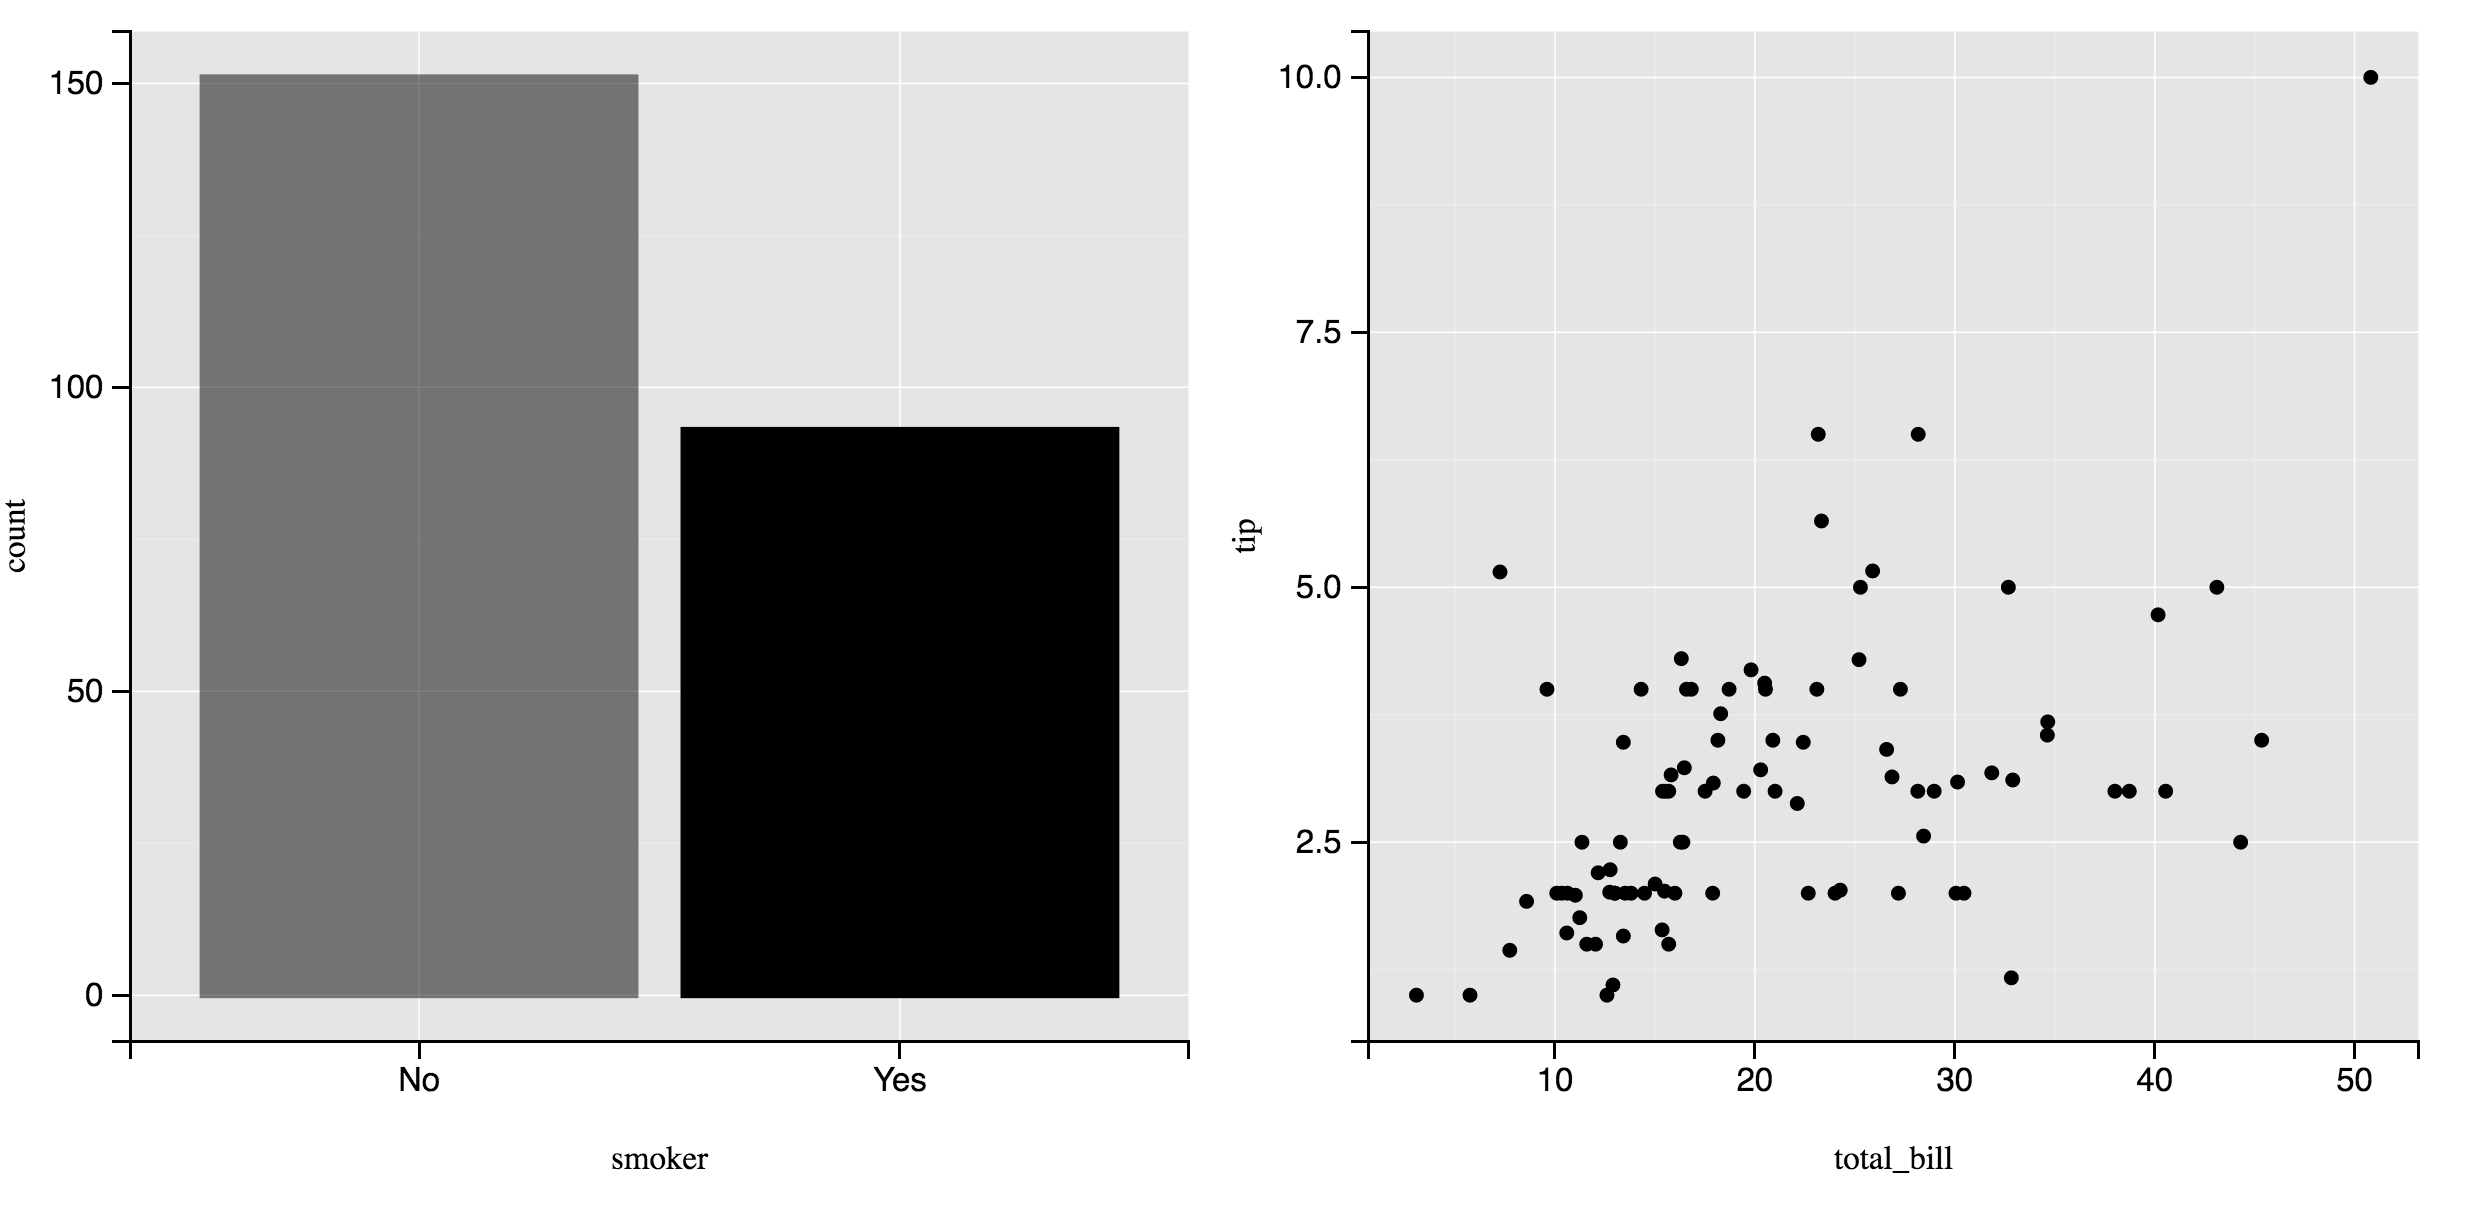
\includegraphics{images/tips}
\caption{\label{fig:tips}Linked database querying via direct manipulation
using animint. A video demonstration can be viewed online at
\url{https://vimeo.com/160496419}}
\end{figure}

In essense, the R code above allows us to use direct manipulation to
dynamically perform SQL queries of the form:

\begin{Shaded}
\begin{Highlighting}[]
\KeywordTok{SELECT} \NormalTok{total_bill, tip }\KeywordTok{FROM} \NormalTok{tips}
  \KeywordTok{WHERE} \NormalTok{smoker }\KeywordTok{IN} \NormalTok{clickSelects}
\end{Highlighting}
\end{Shaded}

In this example, \texttt{clickSelects} is either ``Yes'' or ``No'', but
as we show in later examples, \texttt{clickSelects} can also be an array
of values. Although \texttt{clickSelects} is tied to a mouseclick event,
this same framework supports other selection events, such as hover or
click+drag. Statistically speaking, this is useful for visualizing and
navigating through joint distributions conditional upon discrete values.
In this sense, our extension is closely related to the same a basis
which leads to trellis displays (Richard A. Becker
\protect\hyperlink{ref-trellis}{1996}) and linked scatterplot brushing
(Becker and Cleveland
\protect\hyperlink{ref-brushing-scatterplots}{1987}). The major
differences are that conditioning: is layer (i.e., not plot) specific,
is not tied to a particular geometry, and can be controlled through
direct manipulation or animation controls. \%\% TODO: make connections
to scagnostics? trelliscope?

\subsection{Adding animation}
\label{sec:animation}

In some sense, the \texttt{showSelected} aesthetic splits the layer into
subsets -- one for every unique value of the \texttt{showSelected}
variable. The \texttt{clickSelects} aesthetics provides a mechanism to
alter the visibility of those subset(s) via direct manipulation, but our
system also provides a mechanism for automatically looping through
selections to produce animation(s). We acheive this by reserving the
name \texttt{time} to specify which variable to select as well as the
amount of time to wait before changing the selection (in milliseconds).
We also reserve the name \texttt{duration} to specify the amount of time
used to smoothly transition between frames (with linear easing). The
code below was used to generate Figure \ref{fig:animation} which
demonstrates a simple animation with smooth transitions between 10
frames of a single point. Note that the resulting web page has controls
for interactively altering the \texttt{time} and \texttt{duration}
parameters.

\begin{Shaded}
\begin{Highlighting}[]
\NormalTok{d <-}\StringTok{ }\KeywordTok{data.frame}\NormalTok{(}\DataTypeTok{v =} \DecValTok{1}\NormalTok{:}\DecValTok{10}\NormalTok{)}
\NormalTok{plotList <-}\StringTok{ }\KeywordTok{list}\NormalTok{(}
  \DataTypeTok{plot =} \KeywordTok{ggplot}\NormalTok{() +}\StringTok{ }\KeywordTok{geom_point}\NormalTok{(}
    \DataTypeTok{data =} \NormalTok{d, }\KeywordTok{aes}\NormalTok{(}\DataTypeTok{x=}\NormalTok{v, }\DataTypeTok{y=}\NormalTok{v, }\DataTypeTok{showSelected=}\NormalTok{v)}
  \NormalTok{),}
  \DataTypeTok{time =} \KeywordTok{list}\NormalTok{(}\DataTypeTok{variable =} \StringTok{"v"}\NormalTok{, }\DataTypeTok{ms =} \DecValTok{1000}\NormalTok{),}
  \DataTypeTok{duration =} \KeywordTok{list}\NormalTok{(}\DataTypeTok{v =} \DecValTok{1000}\NormalTok{)}
\NormalTok{)}
\KeywordTok{animint2dir}\NormalTok{(plotList)}
\end{Highlighting}
\end{Shaded}

\begin{figure}
\centering
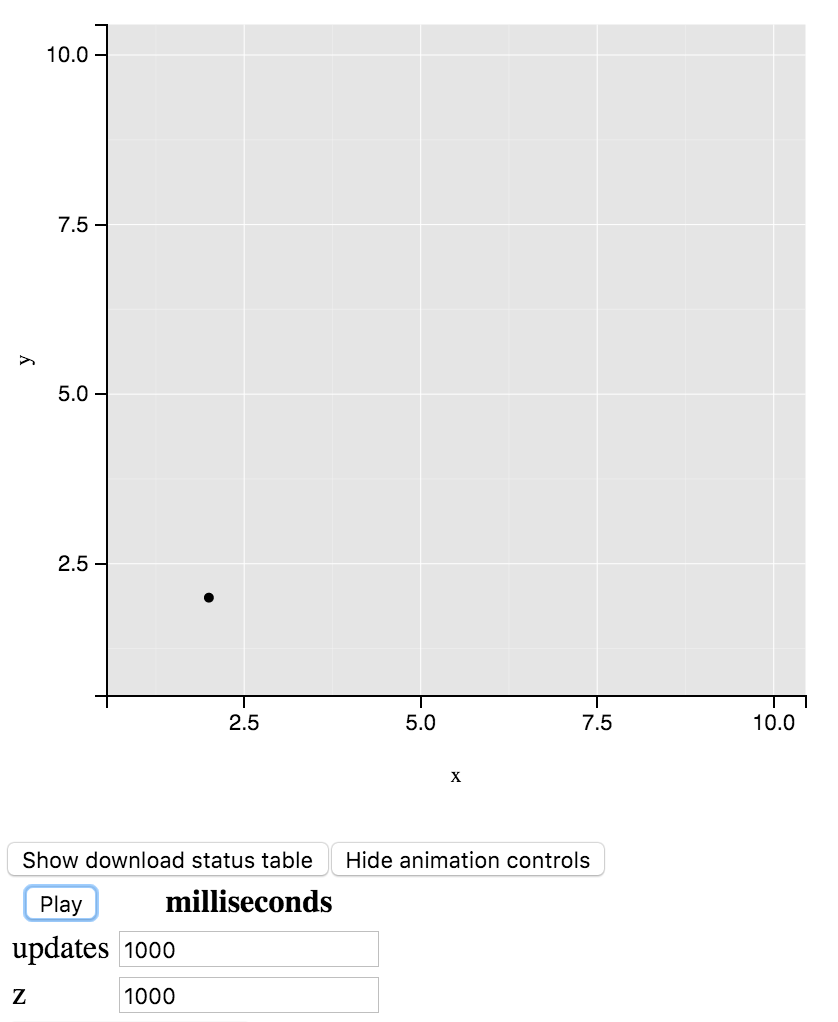
\includegraphics{images/animation}
\caption{\label{fig:animation}A simple animation with smooth transitions and
interactively altering transition durations. A video demonstration can
be viewed online at \url{https://vimeo.com/160505146}}
\end{figure}

\subsection{World Bank Example}
\label{sec:worldbank}

Figure \ref{fig:worldbank} shows an interactive animation of the World
Bank data set (World Bank \protect\hyperlink{ref-WorldBank}{2012})
created with our animint implementation. The visualization helps us
explore the change in the relationship between life expectancy and
fertility over time for 205 countries. By default, the year 1979 and the
countries United States and Vietnam are selected, but readers are
encouraged to watch the video of the animation and/or interact the
visualization using a web
browser.\footnote{\url{http://bl.ocks.org/tdhock/raw/8ce47eebb3039263878f/}}
In the interactive version, the selected value of the year variable is
automatically incremented every few seconds, using animation to
visualize yearly changes in the relationship between life expectancy and
fertility rate.

\begin{figure}
\centering
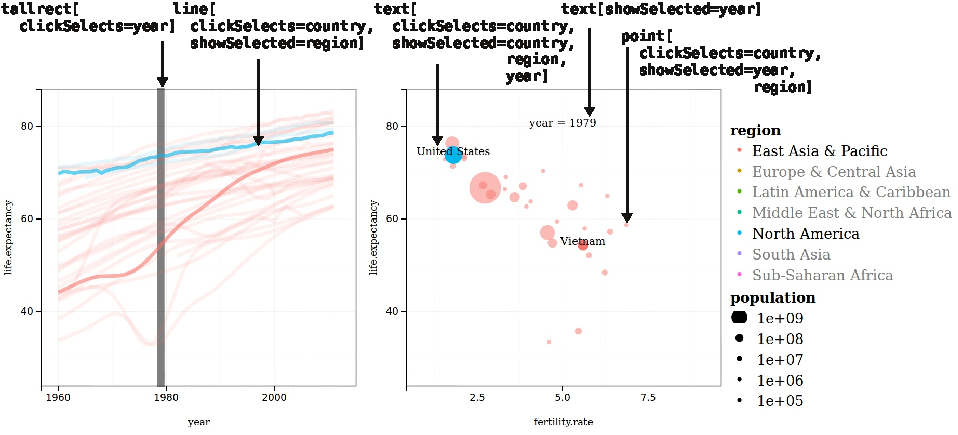
\includegraphics{images/figure-1.pdf}
\caption{\label{fig:worldbank}An interactive animation of World Bank
demographic data of several countries, designed using
\texttt{clickSelects} and \texttt{showSelected} keywords (top). Left: a
multiple time series from 1960 to 2010 of life expectancy, with bold
lines showing the selected countries and a vertical grey tallrect
showing the selected year. Right: a scatterplot of life expectancy
versus fertility rate of all countries. The legend and text elements
show the current selection: year=1979, country= \{United States,
Vietnam\}, and region=\{East Asia \& Pacific, North America\}}
\end{figure}

When viewing the interactive version of Figure \ref{fig:worldbank},
suppose we wish to select Thailand. Direct manipulation is not very
useful in this case since it is not easy to identify and select Thailand
based on graphical marks on a plot. For this reason, animint also
provides dropdown menu(s) for each selection variable to aid the
selection process. Figure \ref{fig:widgets} shows what the user sees
after typing ``th'' in the search box. Note that these dropdowns support
selection of multiple values and coordinate sensibly with selections
made via direct manipulation.

\begin{figure}
\centering
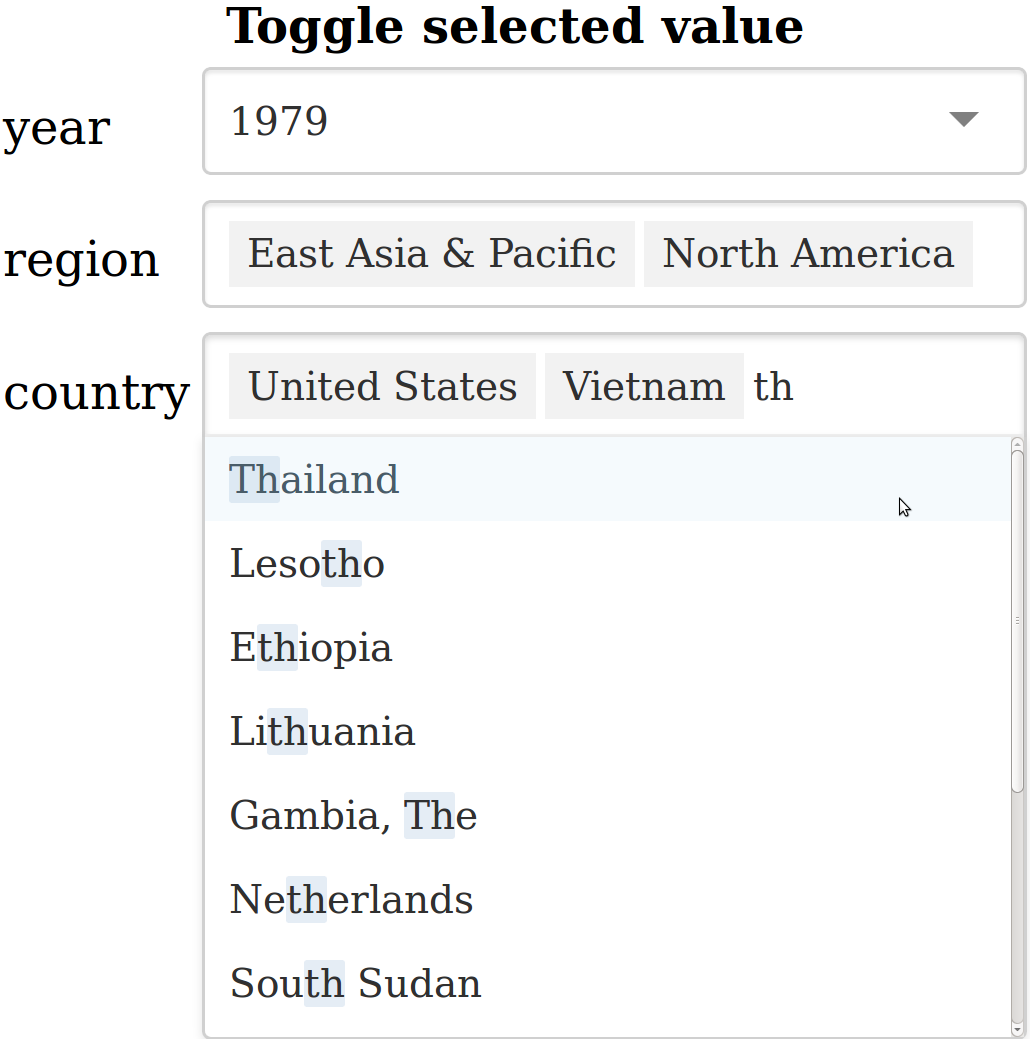
\includegraphics{images/Screenshot-toggle-selected-value}
\caption{\label{fig:widgets}Animint provides a menu to update each selection
variable. In this example, after typing `th' the country menu shows the
subset of matching countries.}
\end{figure}

We anticipate that some ggplot2 users will be able to reverse engineer
the animint code which creates Figure \ref{fig:worldbank}, simply by
looking at it. In fact, this is a big reason why ggplot2 is so widely
used: it helps minimize the amount of time required to translate a
figure that exists in your head into computer code. Note that, in the
left hand plot of Figure \ref{fig:worldbank}, we have a time series of
the life expectancy where each line is a country (i.e., we
\texttt{group} by country) and lines are colored by region. By clicking
on a line, we also want the country label to appear in the right hand
plot, so we also need to set \texttt{clickSelects=country}. Lastly, by
setting \text{showSelected=region}, we can hide/show lines by clicking
on the color legend entries.

\begin{Shaded}
\begin{Highlighting}[]
\NormalTok{timeSeries <-}\StringTok{ }\KeywordTok{ggplot}\NormalTok{() +}\StringTok{ }\KeywordTok{geom_line}\NormalTok{(}
  \DataTypeTok{data =} \NormalTok{WorldBank,}
  \KeywordTok{aes}\NormalTok{(}\DataTypeTok{x =} \NormalTok{year, }\DataTypeTok{y =} \NormalTok{life.expectancy,}
      \DataTypeTok{group =} \NormalTok{country, }\DataTypeTok{color =} \NormalTok{region,}
      \DataTypeTok{clickSelects =} \NormalTok{country, }
      \DataTypeTok{showSelected =} \NormalTok{region)}
\NormalTok{)}
\end{Highlighting}
\end{Shaded}

We want to provide a visual clue for the selected year in the time
series, so we also layer some ``tall rectangles" onto the time series.
These tall rectangles will also serve as a way to directly modify the
selected year. The tallrect geometry is a special case of a rectangle
that automatically spans the entire vertical range, so we just have to
specify the horizontal range via \texttt{xmin} and \texttt{xmax}. Also,
since the layered grammar of graphics allows for different data in each
layer, we supply a data frame with just the unique years in the entire
data for this layer.

\begin{Shaded}
\begin{Highlighting}[]
\NormalTok{years <-}\StringTok{ }\KeywordTok{data.frame}\NormalTok{(}\DataTypeTok{year =} \KeywordTok{unique}\NormalTok{(WorldBank$year))}
\NormalTok{timeSeries <-}\StringTok{ }\NormalTok{timeSeries +}\StringTok{ }\KeywordTok{geom_tallrect}\NormalTok{(}
  \DataTypeTok{data =} \NormalTok{years,}
  \KeywordTok{aes}\NormalTok{(}\DataTypeTok{xmin =} \NormalTok{year -}\StringTok{ }\FloatTok{0.5}\NormalTok{, }\DataTypeTok{xmax =} \NormalTok{year +}\StringTok{ }\FloatTok{0.5}\NormalTok{,}
      \DataTypeTok{clickSelects =} \NormalTok{year)}
\NormalTok{)}
\end{Highlighting}
\end{Shaded}

As for the right hand plot in Figure \ref{fig:worldbank}, there are
three layers: a point layer for countries, a text layer for countries,
and a text layer to display the selected year. By clicking on a point,
we want to display the country text label and highlight the
corresponding time series on the right hand plot, so we set
\texttt{clickSelects=country} in this layer. Furthermore, we only want
to show the points for the selected year and region, so we also need
\texttt{showSelected=year} and \texttt{showSelected2=region}.

\begin{Shaded}
\begin{Highlighting}[]
\NormalTok{scatterPlot <-}\StringTok{ }\KeywordTok{ggplot}\NormalTok{() +}\StringTok{ }\KeywordTok{geom_point}\NormalTok{(}
  \DataTypeTok{data =} \NormalTok{WorldBank,}
  \KeywordTok{aes}\NormalTok{(}\DataTypeTok{x =} \NormalTok{fertility.rate, }\DataTypeTok{y =} \NormalTok{life.expectancy,}
      \DataTypeTok{color =} \NormalTok{region, }\DataTypeTok{size =} \NormalTok{population,}
      \DataTypeTok{clickSelects =} \NormalTok{country,}
      \DataTypeTok{showSelected =} \NormalTok{year,}
      \DataTypeTok{showSelected2 =} \NormalTok{region)}
\NormalTok{)}
\end{Highlighting}
\end{Shaded}

The text layer for annotating selected countries is essentially the same
as the point layer, except we map the country name to the \texttt{label}
aesthetic.

\begin{Shaded}
\begin{Highlighting}[]
\NormalTok{scatterPlot <-}\StringTok{ }\NormalTok{scatterPlot +}\StringTok{ }\KeywordTok{geom_text}\NormalTok{(}
  \DataTypeTok{data =} \NormalTok{WorldBank,}
  \KeywordTok{aes}\NormalTok{(}\DataTypeTok{x =} \NormalTok{fertility.rate, }\DataTypeTok{y =} \NormalTok{life.expectancy,}
      \DataTypeTok{label =} \NormalTok{country,}
      \DataTypeTok{showSelected =} \NormalTok{country,}
      \DataTypeTok{showSelected2 =} \NormalTok{year,}
      \DataTypeTok{showSelected3 =} \NormalTok{region)}
\NormalTok{)}
\end{Highlighting}
\end{Shaded}

Lastly, to help identify the selected year when viewing the scatterplot,
we add another layer of text at a fixed location.

\begin{Shaded}
\begin{Highlighting}[]
\NormalTok{scatterPlot <-}\StringTok{ }\NormalTok{scatterPlot +}\StringTok{ }\KeywordTok{geom_text}\NormalTok{(}
  \DataTypeTok{data =} \NormalTok{years, }\DataTypeTok{x =} \DecValTok{5}\NormalTok{, }\DataTypeTok{y =} \DecValTok{80}\NormalTok{,}
  \KeywordTok{aes}\NormalTok{(}\DataTypeTok{label =} \KeywordTok{paste}\NormalTok{(}\StringTok{"year ="}\NormalTok{, year),}
      \DataTypeTok{showSelected =} \NormalTok{year)}
\NormalTok{)}
\end{Highlighting}
\end{Shaded}

Now that we have defined the plots in Figure \ref{fig:worldbank}, we can
set the \texttt{time} and \texttt{duration} options (introduced in
Section \ref{sec:animation}) to control the animation parameters. Our
animint implementation also respects a \texttt{selector.types} option
which controls whether or not selections for a given variable can
accumulate and a \texttt{first} option for controlling which values are
selected by default.
\footnote{We maintain a complete list of (animint specific) options here --
\url{https://github.com/tdhock/animint/wiki/Advanced-features-present-animint-but-not-in-ggplot2}}
By default, supplying the list of plots and additional options to
\texttt{animint2dir()} will write all the files necessary to render the
visualization to a temporary directory and prompt a web browser to open
an HTML file.

\begin{Shaded}
\begin{Highlighting}[]
\NormalTok{viz <-}\StringTok{ }\KeywordTok{list}\NormalTok{(}
  \DataTypeTok{timeSeries =} \NormalTok{timeSeries,}
  \DataTypeTok{scatterPlot =} \NormalTok{scatterPlot,}
  \DataTypeTok{time =} \KeywordTok{list}\NormalTok{(}\DataTypeTok{variable =} \StringTok{"year"}\NormalTok{, }\DataTypeTok{ms =} \DecValTok{3000}\NormalTok{),}
  \DataTypeTok{duration =} \KeywordTok{list}\NormalTok{(}\DataTypeTok{year =} \DecValTok{1000}\NormalTok{),}
  \DataTypeTok{selector.types =} \KeywordTok{list}\NormalTok{(}
    \DataTypeTok{year =} \StringTok{"single"}\NormalTok{,}
    \DataTypeTok{country =} \StringTok{"multiple"}\NormalTok{,}
    \DataTypeTok{region =} \StringTok{"multiple"}
  \NormalTok{),}
  \DataTypeTok{first =} \KeywordTok{list}\NormalTok{(}
    \DataTypeTok{country =} \KeywordTok{c}\NormalTok{(}\StringTok{"United States"}\NormalTok{, }\StringTok{"Thailand"}\NormalTok{)}
  \NormalTok{)}
\NormalTok{)}
\KeywordTok{animint2dir}\NormalTok{(viz)}
\end{Highlighting}
\end{Shaded}

\subsection{Implementation details}
\label{sec:implementation}

As shown in Figure \ref{fig:design}, the animint system is implemented
in 2 parts: the compiler and the renderer. The compiler is implemented
in about 2000 lines of R code that converts a list of ggplots and
options to a JSON plot meta-data file and a tab-separated values (TSV)
file database.

\begin{figure}
\centering
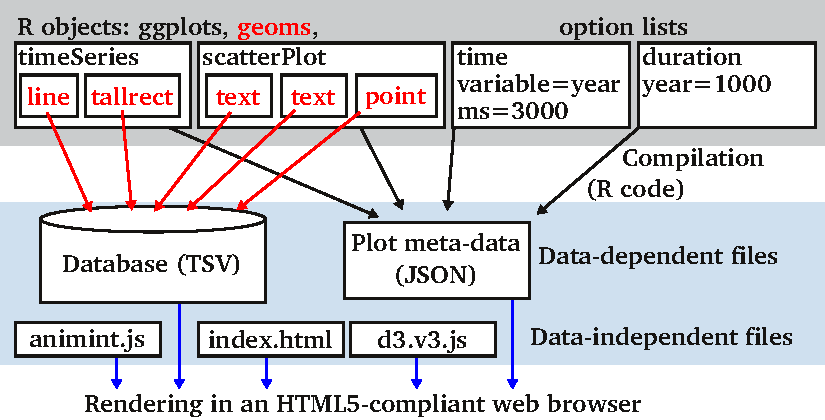
\includegraphics{images/figure-design.pdf}
\caption{\label{fig:design}A schematic explanation of compilation and
rendering in the World Bank visualization. Top: the interactive
animation is a list of 4 R objects: 2 ggplots and 2 option lists.
Center: animint R code compiles data in ggplot geoms to a database of
TSV files (\textcolor{red}{$\rightarrowtriangle$}). It also compiles
plot meta-data including ggplot aesthetics, animation time options, and
transition duration options to a JSON meta-data file
(\(\rightarrowtriangle\)). Bottom: those data-dependent compiled files
are combined with data-independent JavaScript and HTML files which
render the interactive animation in a web browser
(\textcolor{blue}{$\rightarrowtriangle$}).}
\end{figure}

\begin{figure}
\centering
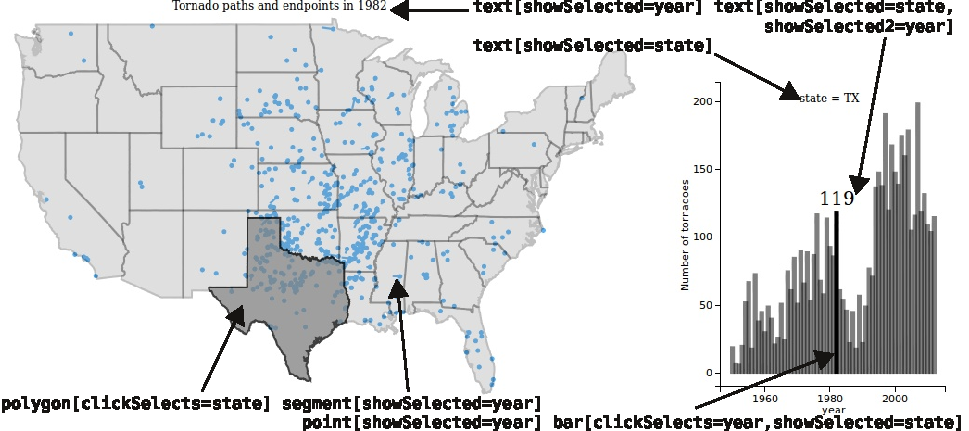
\includegraphics{images/figure-tornado.pdf}
\caption{\label{fig:tornado}Interactive animation of tornadoes recorded from
1950 to 2012 in the United States. Left: map of the lower 48 United
States with tornado paths in 1982. The text shows the selected year, and
clicking the map changes the selected state, currently Texas. Right:
time series of tornado counts in Texas. Clicking a bar changes the
selected year, and the text shows selected state and the number of
tornadoes recorded there in that year (119 tornadoes in Texas in 1982).}
\end{figure}

\begin{figure}
\centering
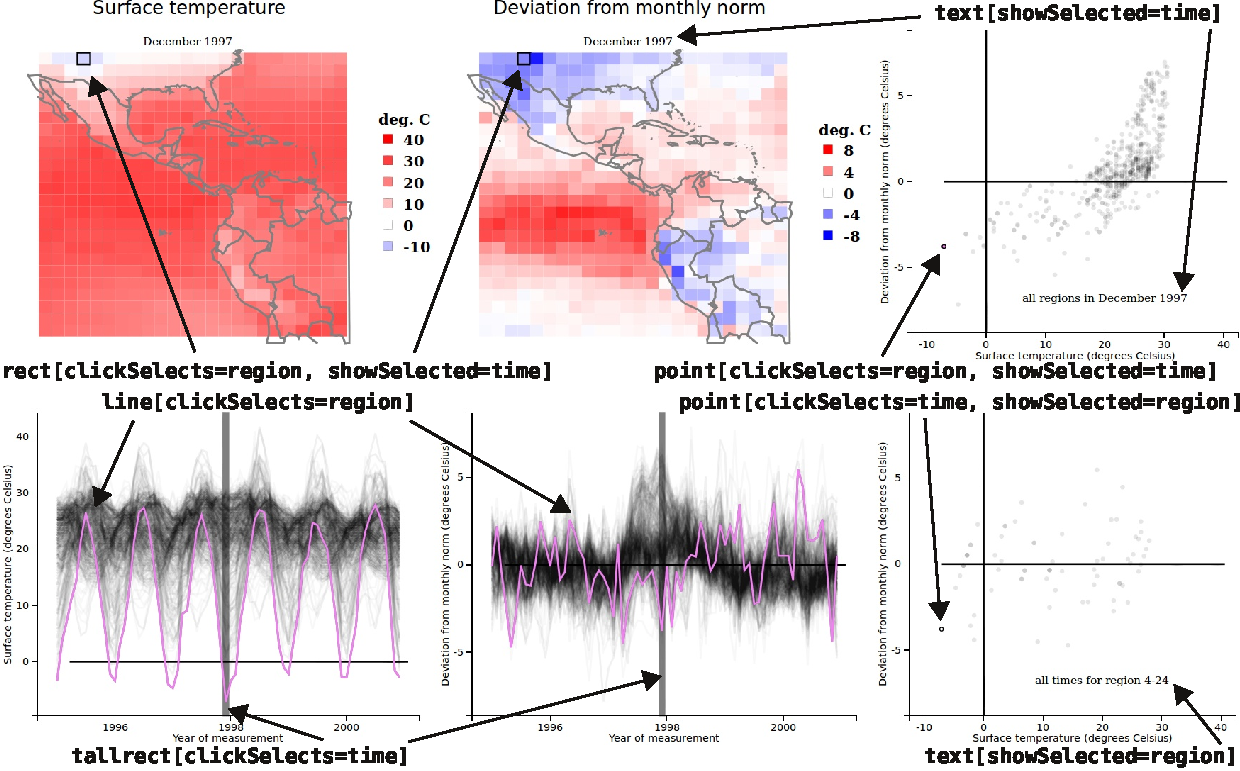
\includegraphics{images/figure-climate.pdf}
\caption{\label{fig:climate}Visualization containing 6 linked, interactive,
animated plots of Central American climate data. Top: for the selected
time (December 1997), maps displaying the spatial distribution of two
temperature variables, and a scatterplot of these two variables. The
selected region is displayed with a black outline, and can be changed by
clicking a rect on the map or a point on the scatterplot. Bottom: time
series of the two temperature variables with the selected region shown
in violet, and a scatterplot of all times for that region. The selected
time can be changed by clicking a background tallrect on a time series
or a point on the scatterplot. The selected region can be changed by
clicking a line on a time series.}
\end{figure}

The compiler scans the aesthetics in the ggplots to determine how many
selection variables are present, and which geoms to update after a
selection variable is updated. It uses ggplot2 to automatically
calculate the axes scales, legends, labels, backgrounds, and borders. It
outputs this information to the JSON plot meta-data file.

The compiler also uses ggplot2 to convert data variables (e.g.~life
expectancy and region) to visual properties (e.g.~y position and color).
The data for each layer/geom are saved in several TSV files, one for
each combination showSelected values. Thus for large data sets, the web
browser only needs to download the subset of data required to render the
current selection (Heer \protect\hyperlink{ref-2013-immens}{2013}).

When repeated data would be saved in each of the TSV files, an extra
common TSV file is created so that the repeated data only need to be
stored and downloaded once. In that case, the other TSV files do not
store the common data, but are merged with the common data after
downloading. This method for constructing the TSV file database was
developed to minimize the disk usage of animint, particularly for
ggplots of spatial maps as in Figure \ref{fig:tornado}.

Finally, the rendering engine (\texttt{index.html}, \texttt{d3.v3.js},
and \texttt{animint.js} files) is copied to the plot directory. The
\texttt{animint.js} renderer is implemented in about 2200 lines of
JavaScript/D3 code that renders the TSV and JSON data files as SVG in a
web browser. Importantly, animation is achieved by using the JavaScript
\texttt{setInterval} function, which updates the \texttt{time} selection
variable every few seconds. Since the compiled plot is just a directory
of files, the interactive plots can be hosted on any web server. The
interactive plots can be viewed by opening the \texttt{index.html} page
in any modern web browser.

\section{Exploring performance \& scope with examples}
\label{sec:performance}

This section attempts to demonstrate a range of visualizations that are
supported by animint with more examples. Figure \ref{fig:tornado} shows
an interactive animation of tornadoes observed in the United States
between 1950 and 2012. At any moment in time, the user can
simultaneously view the spatial distribution of tornadoes in the
selected year over all states, and see the trend over all years for the
selected state. Clicking a state on the map updates the time series bars
to show the tornado counts from that state. Clicking a bar on the time
series updates the selected year. Figure \ref{fig:climate} shows an
interactive animation of climate time series data observed in Central
America. Two maps display the spatial distribution of two temperature
variables, which are shown over time in corresponding the time series
plots below. Scatterplots also show the relationships between the two
temperature variables for the selected time and region. Clicking any of
the plots updates all 6 of them. The \texttt{clickSelects} and
\texttt{showSelected} aesthetics make it easy to design this set of 6
linked plots in only 87 lines of code.

Summary statistics describing complexity and performance for examples in
this paper, as well as other animint examples, are displayed in Table
\ref{tab:examples}. The climate data visualization has noticeably slow
animations, since it displays about 88,980 geometric elements at once
(\url{http://bit.ly/QcUrhn}). We observed this slowdown across all
browsers, which suggested that there is an inherent bottleneck when
rendering large interactive plots in web browsers using JavaScript and
SVG. Another animint with a similar amount of total rows is based on the
evolution data (\url{http://bit.ly/O0VTS4}), but since it shows less
data onscreen (about 2703 elements), it exhibits faster responses to
interactivity and animation.

Animint is still useful for creating interactive but non-animated plots
when there is not a time variable in the data. In fact, 7 of the 11
examples in Table \ref{tab:examples} are not animated. For example,
linked plots are useful to illustrate complex concepts such as a change
point detection model in the breakpoints data
(\url{http://bit.ly/1gGYFIV}). The user can explore different model
parameters and data sets since these are encoded as animint interaction
variables.

\begin{table*}[htp] % This table is too wide to fill in the page.
  \centering
  \hspace*{-2cm}
  % latex table generated in R 3.1.1 by xtable 1.7-3 package
% Thu Oct  9 14:20:02 2014
\begin{tabular}{rrrrrrrrrrr}
  \hline
 & LOC & seconds & MB & rows & onscreen & variables & interactive & plots & animated? & Fig \\ 
  \hline
worldPop & 17 & 0.2 & 0.1 & 924 & 624 &  4 &  2 &  2 & yes &  \\ 
  WorldBank & 20 & 2.3 & 2.1 & 34132 & 11611 &  6 &  2 &  2 & yes &  \ref{fig:worldbank} \\ 
  evolution & 25 & 21.6 & 12.0 & 240600 & 2703 &  5 &  2 &  2 & yes &  \\ 
  change & 36 & 2.8 & 2.5 & 36238 & 25607 & 12 &  2 &  3 & no &  \\ 
  tornado & 39 & 1.7 & 6.1 & 103691 & 16642 & 11 &  2 &  2 & no &  \ref{fig:tornado} \\ 
  prior & 54 & 0.7 & 0.2 & 1960 & 142 & 12 &  3 &  4 & no &  \\ 
  compare & 66 & 10.7 & 7.9 & 133958 & 2140 & 20 &  2 &  5 & no &  \\ 
  breakpoints & 68 & 0.5 & 0.3 & 4242 & 667 & 13 &  2 &  3 & no &  \\ 
  climate & 84 & 12.8 & 19.7 & 253856 & 88980 & 15 &  2 &  6 & yes &  \ref{fig:climate} \\ 
  scaffolds & 110 & 56.3 & 78.5 & 618740 & 9051 & 30 &  3 &  3 & no &  \\ 
  ChIPseq & 229 & 29.9 & 78.3 & 1292464 & 1156 & 44 &  4 &  5 & no & \\ 
   \hline
\end{tabular}

  \vskip 0.2cm
  \caption{Characteristics of 11 interactive visualizations designed with
    animint. The interactive version of these visualizations can be accessed 
    via \url{http://sugiyama-www.cs.titech.ac.jp/\~toby/animint/}.
    From left to right, we show the data set name, the
    lines of R code (LOC) including data processing but not including comments
    (80 characters max per line),
    the amount of time it takes to compile the visualization (seconds),
    the total size of the uncompressed TSV files in megabytes (MB),
    the total number of data points (rows),
    the median number of data points shown at once (onscreen),
    the number of data columns visualized (variables),
    the number of \texttt{clickSelects}/\texttt{showSelected} 
    variables (interactive),
    the number of linked panels (plots),
    if the plot is animated,
    and the corresponding Figure number in this paper (Fig).
  }
\label{tab:examples}
\end{table*}

\section{Comparison study}
\label{sec:compare}

In this section we compare our animint implementation with other similar
leading systems by creating a given visualization in each system and
discussing the pros and cons of the different approaches.

\subsection{The Grand Tour}
\label{sec:tour}

The Grand Tour is a well-known method for viewing high dimensional data
which requires interactive and dynamic graphics (Asimov
\protect\hyperlink{ref-grand-tour}{1985}). Figure \ref{fig:tour} shows a
grand tour of 300 observations sampled from a correlated tri-variate
normal distribution. The left hand view shows the marginal density of
each point while the right hand view ``tours" through 2D projections of
the 3D data. There are many ways to choose projections in a tour, and
many ways to interpolate between projections, most of which can be
programmed fairly easily using R and relevant add-on packages. In this
case, we used the R package tourr, which uses the geodesic random walk
(i.e., random 2D projection with geodesic interpolation) in its grand
tour algorithm (Wickham et al. \protect\hyperlink{ref-tourr}{2011}).

\begin{figure}
\centering
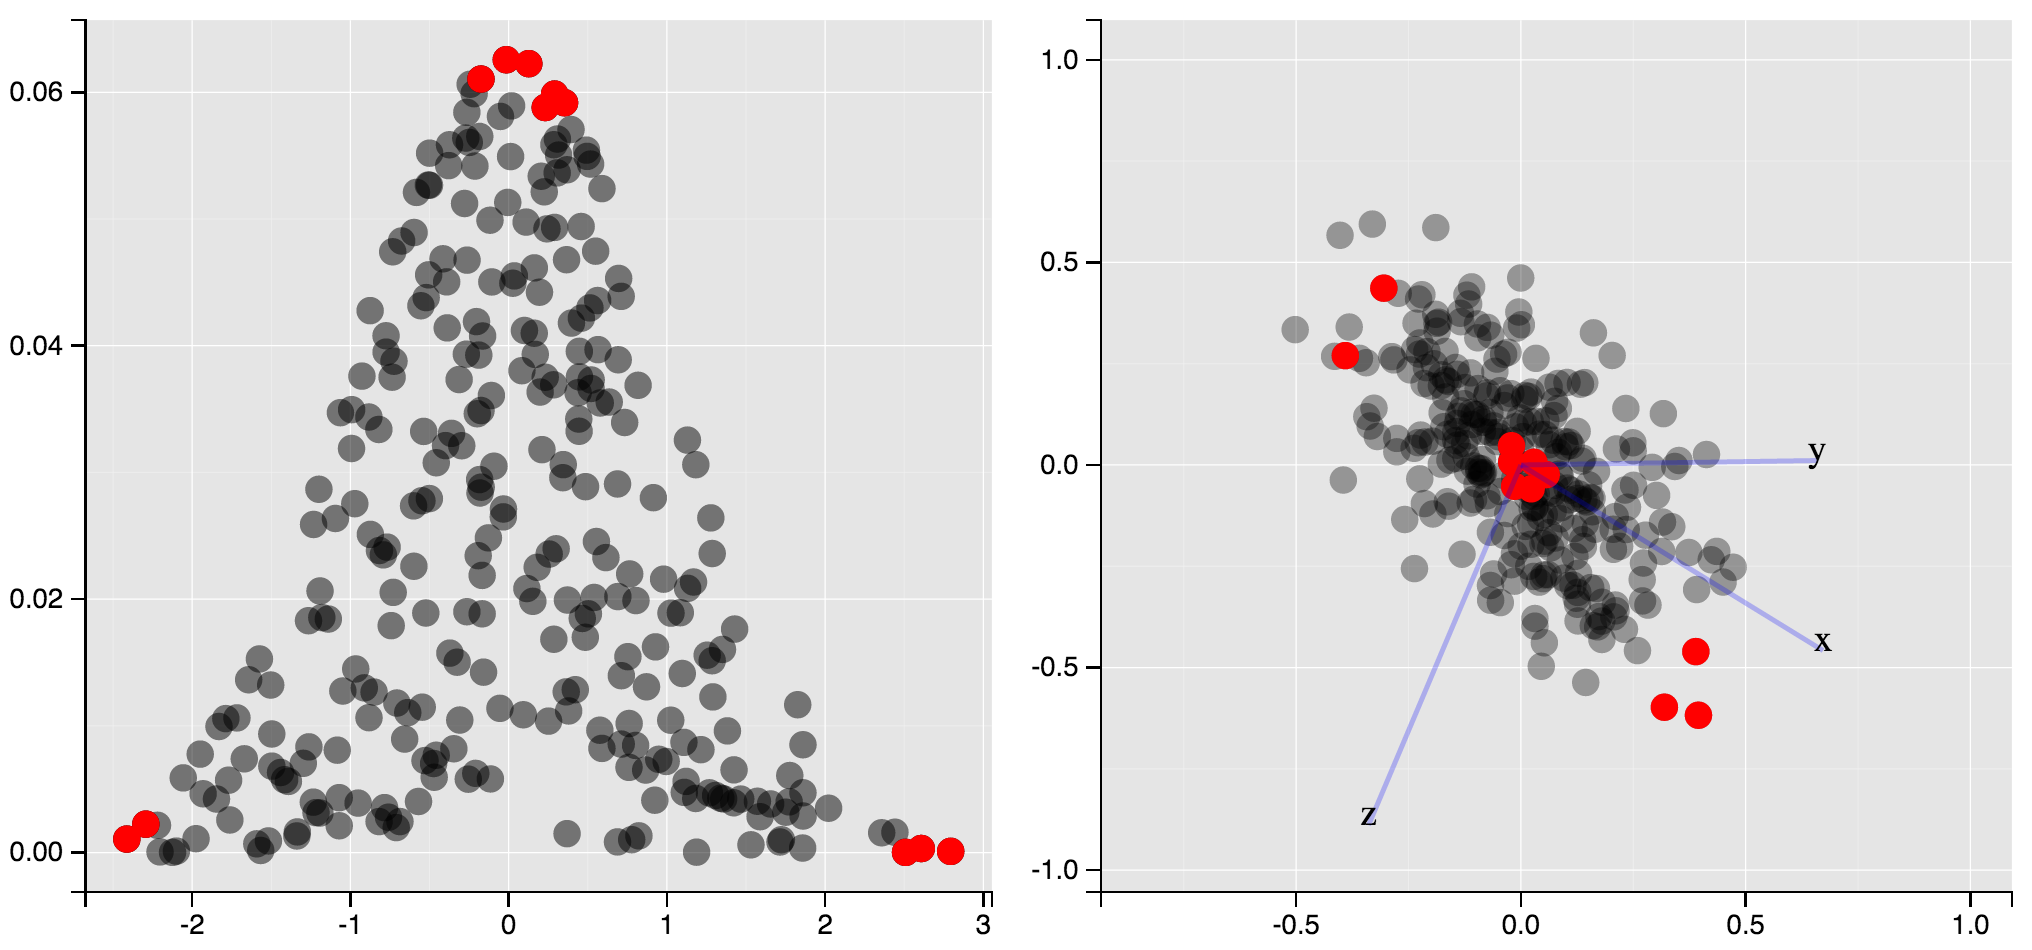
\includegraphics{images/tour}
\caption{\label{fig:tour}Linked selection in a grand tour with animint. A
video demonstration can be viewed online at
\url{https://vimeo.com/160720834}}
\end{figure}

When touring data, it is generally useful to link low-dimensional
displays with the tour itself. The video in Figure \ref{fig:tour} was
generated with our current animint implementation, and points are
selected via mouse click which reveal that points with high marginal
density are located in the ellipsoid center while points with a low
marginal density appear near the ellipsoid border. In this case, it
would be convenient to also have brush selection, as we demonstrate in
Figure \ref{fig:tourbrush} which implements the same touring example
using the R packages ggvis and shiny. The brush in Figure
\ref{fig:tourbrush} is implemented with shiny's support for brushing
static images, which currently does not support multiple brushes, making
it difficult to select non-contiguous regions.

\begin{figure}
\centering
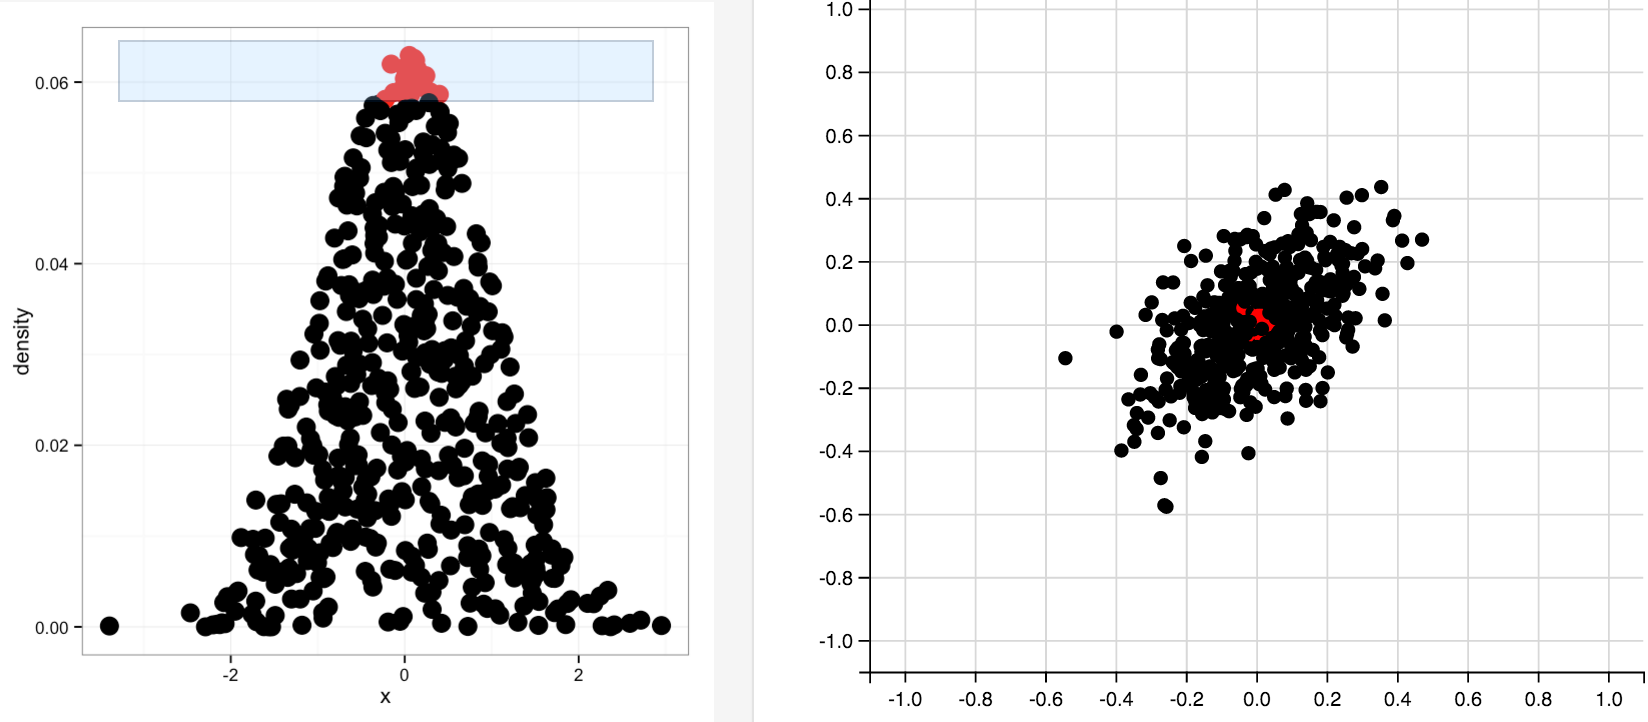
\includegraphics{images/tourbrush}
\caption{\label{fig:tourbrush}Linked selection in a grand tour with ggvis
and shiny. A video demonstration can be viewed online at
\url{https://vimeo.com/160825528}}
\end{figure}

This example helps point out a few other important differences in using
animint versus ggvis+shiny to implement ``multiple linked and dynamic
views" as described in (Ahlberg, Williamson, and Shneiderman
\protect\hyperlink{ref-Ahlberg:1991}{1991}) and (Buja et al.
\protect\hyperlink{ref-Buja:1991vh}{1991}). Maintaining state of the
linked brush in Figure \ref{fig:tourbrush} requires both knowledge and
clever use of some sophicated programming techniques such as closures
and reactivity. It also requires knowledge of the shiny web application
framework and a new approach to the grammar of graphics. On the other
hand, maintaining state in Figure \ref{fig:tour} requires a few
different \texttt{clickSelects}/\texttt{showSelected} mappings. As a
result, we believe animint provides a more elegant user interface for
this application.

The tourring example also helps point out important consequences of the
design and implementation of these two different systems. As mentioned
in Section \ref{sec:implementation}, our current animint implementation
requires every subset of data to be precomputed before render time. For
visualizations such as tours, where it is more efficient to perform
statistical computations on-the-fly, this can be a harsh restriction,
but this is a restriction of our current implementation (not a
restriction of the framework itself). As a result, when touring a large
high-dimensional space, where many projections are needed, ggvis+shiny
may be desirable since the projections are computed on the server and
sent to the browser in real-time. This works fine when the application
is running and viewed on the same host machine, but viewing such an
application hosted on a remote machine can produce staggered animations
since client-server requests must be performed, processed, and rendered
roughly 30 times a second. Also, generally speaking, the animint system
results a more pleasant experience when it comes to hosting and sharing
applications since it doesn't require a Web Server with R and special
software already installed.

\subsection{World Bank Example}

We also recreated Figure \ref{fig:worldbank} using ggvis+shiny (see
\url{http://bit.ly/1SsJKlN}) and Tableau (see
\url{http://bit.ly/worldBank-tableau}). Even as experienced ggvis+shiny
users, we found it quite difficult to replicate this example, and were
not able completely replicate it due to a lack of a mechanism for
coordinating indirect and direct manipulations. Overall the
visualization is pretty similar, but lacks a few important features. In
particular, there is no way to control the selected year using both the
slider (indirect) and clicking on the ggvis plot (direct). It also lacks
the ability to click on a countries time series and label the
corresponding point on the scatterplot. This might be possible, but we
could not find a way to update a plot based on a click event on a
different plot. Even with this lack of functionality, the ggvis+shiny is
significantly more complicated and requires more code (about 100 lines
of code compared to 30).

It was also impossible to completely replicate Figure
\ref{fig:worldbank} using Tableau essentially because the example
requires a \emph{layered} approach to the grammar of graphics. In
particular, since graphical marks and interaction source/target(s) must
derive from the same table in Tableau, it was impossible to control the
clickable multiple time series and the clickable tallrects in different
ways based on the two different selection variables. In other words, in
Tableau, selections are managed on the plot level, but in animint,
selections are specific to each graphical layer.

\section{User feedback and observations}

By working with researchers in several fields of research, we have
created a wide variety of interactive visualizations using animint.
Typically, the researchers have a complex data set that they wish to
visualize, but they do not have the expertise or time to create an
interactive data visualization. The animint system made it easy to
collaborate with the various domain experts, who were able to provide us
with annotated sketches of the desired plots, which we then translated
to animint R code. In this section we share comments and constructive
criticism that we have obtained from our users.

\subsection{User perspective}

For the \texttt{prior} data visualization (\url{http://bit.ly/1peIT7t}),
the animint user is a machine learning researcher who developed an
algorithm and applied it to 4 benchmark data sets. He wanted to explore
how his algorithm performed, in comparison to a baseline learning
algorithm. He appreciated the intuition about his algorithm's
performance that he learned from the interactive plots: ``Interactive
plotting allows us to explore all relationships of our high-dimensional
dataset and gives us an intuitive understanding of the performance of
our proposed algorithm. An intuitive understanding of the results is
important since it shows under which conditions our proposed method
works well and provides avenues for further research.''

Another user from a machine learning background found the interactive
plots useful for presenting his work: `\texttt{the}regularization path'
is a difficult concept to demonstrate in my research. The animint
(\url{http://bit.ly/1gVb8To}) helped greatly by rendering an interactive
plot of regularization path, likelihood, and graph at the same time and
illustrating their connections. It also reveals an interesting
phenomenon that maximizing the testing likelihood actually gives many
false positives.''

In another application, the animint user was a genomics researcher:
``viewing and exploring my complex intestinal microbiome dataset in
animint allowed me to grasp the patterns and relationships between
samples at an almost intuitive level. The interactive aspect of it was
very helpful for browsing through the dataset.''

Finally, users also appreciated the simple web interface, and the detail
that is possible to show in interactive plots, but impossible to show in
publications: ``\ldots{} the web interface is simple and easy to use. It
also enables us to publish more detailed interactive results on our
website to accompany the results presented in publications.''

\subsection{Developer perspective}

R users, and in particular ggplot2 users, have found that animint is
easy to learn and use. One statistics Ph.D.~student writes, ``animint is
a fantastic framework for creating interactive graphics for someone
familiar with R and ggplot2's grammar of graphics implementation. The
API is very intuitive and allows one to quickly bring their static
graphics to life in a way that facilitates exploratory data analysis.''

\section{Limitations and future work}
\label{sec:limitations}

A number of limitations derive from the fact that some plot features are
computed once during the compilation step and remain static on a
rendered plot. For example, users are unable to change variable mappings
after compilation. Also, when different data subsets have very different
ranges of values, it may be preferable to recompute scales when
\texttt{clickSelects} selection(s) change. A future implementation of
animint would benefit from changes to the compiler and renderer that
allow scales to be updated after each click. Some of these limitations
can be resolved by adding interactive widgets to ``recompile" components
hard-coded in the plot meta information. In fact, animint makes it easy
to embed visualizations inside of shiny web applications, and we have an
example of interactively redefining variable mappings
(\url{http://bit.ly/animint-shiny}).

Our compiler also currently takes advantage of ggplot2 internals to
compute statistics and positional adjustments before rendering. As a
result, statistics/positions will not dynamically recompute based on
selections. In other words, using
\texttt{clickSelects}/\texttt{showSelected} with non-identity
statistic(s)/position(s) may not generate a sensible result. It would be
possible, but a significant amount of work, to transfer these
computations from the compiler to the renderer.

Another set of limitations derive our current restriction that all
subsets (corresponding to each possible selection) must be precomputed
before render time. As eluded to in Section \ref{sec:tour}, if there is
a large space of possible selections, it is impractical to precompute
every subset before viewing. Therefore, it would be useful if the
renderer could dynamically compute subsets when new selections are made.

Our implementation is also limited to two specific types of direct
manipulation: selecting graphical elements via mouse click
(\texttt{clickSelects}), and showing/hiding related elements
(\texttt{showSelected}). However, the framework described in Section
\ref{sec:extension} is not restricted to a particular event type, so
\texttt{hoverSelects} and \texttt{brushSelects} aesthetics could be
added, for instance. There are other types of interaction that should be
added, that wouldn't require additional extensions to the grammar of
graphics, such as: zooming, panning, and plot resizing.

\section{Conclusion}

Our R package animint extends ggplot2's layered grammar of graphics
implementation for a declarative approach to producing interactive and
dynamic web graphics. By adding two aesthetics to specify selection
source(s) and target(s), ggplot2 users can quickly and easily create
animations with smooth transitions and perform database queries via
direct manipulation of linked views. As a result, animint is a useful
tool not only for exploratory data analysis, but also for the
presentation and distribution of interactive statistical graphics.

\section*{Acknowledgements}

The authors wish to thank animint users MC Du Plessis, Song Liu,
Nikoleta Juretic, and Eric Audemard who have contributed constructive
criticism and helped its development.

\chapter{Interactive data visualization on the web using R}

\section{Introduction}\label{introduction-1}

Cook, Buja, and Swayne (\protect\hyperlink{ref-Cook:2007uk}{2007})
proposed a taxonomy of interactive data visualization based on three
fundamental data analysis tasks: finding Gestalt, posing queries, and
making comparisons. The top-level of the taxonomy comes in two parts:
\emph{rendering}, or what to show on a plot; and \emph{manipulation}, or
what to do with plots. Under the manipulation branch, they propose three
branches of manipulation: focusing individual views, arranging many
views, and linking multiple views. Of course, each of the three
manipulation branches include a set of techniques for accomplishing a
certain task (e.g., within focusing views: controlling aspect ratio,
zoom, pan, etc), and they provide a series of examples demonstrating
techniques using the XGobi software toolkit (Swayne, Cook, and Buja
\protect\hyperlink{ref-xgobi}{1998}). This paper applies similar
interactive techniques to analyze data from three different sources
using web-based interactive graphics.

Traditionally, interactive graphics software toolkits are available as
desktop applications, but more recently, toolkits have used a web-based
approach. In addition to being easier to share and embed within
documents, a web-based approach opens up more potential for linking
views between different interactive graphics toolkits. This ability
grants a tremendous amount of power to the analyst since they may
combine the strengths of several systems at once. However,
unfortunately, there has been a suprising lack of work done on enabling
graphical queries between multiple views (like the work done by Buja et
al. (\protect\hyperlink{ref-Buja:1991vh}{1991}); Unwin A.
(\protect\hyperlink{ref-MANET}{1996}); Cook, Buja, and Swayne
(\protect\hyperlink{ref-Cook:2007uk}{2007}); Cook and Swayne
(\protect\hyperlink{ref-ggobi:2007}{2007}), but in a web-based
environment).

For a number of years, R users have been able to link arbitrary views
via the \textbf{shiny} package -- a reactive programming framework for
authoring web applications entirely within R (Chang et al.
\protect\hyperlink{ref-shiny}{2015}). Although \textbf{shiny} is a
powerful tool for prototyping, it may introduce unnecessary
computational complexity, and lacks semantics for performing graphical
queries on web-based graphics. As a result, when linking views in a
\textbf{shiny} app, one typically has to resort to a naive updating rule
-- when a query is made, the entire graph has to be redrawn. By adding
semantics for graphical queries, it allows the underlying graphing
libraries to be more intelligent about updating rules which generally
leads to a more responsive graphical query.

The R package \textbf{plotly} is one such project that has semantics for
linking views with and without \textbf{shiny} (Sievert et al.
\protect\hyperlink{ref-plotly}{2016}); (Sievert
\protect\hyperlink{ref-plotly-book}{2016}\protect\hyperlink{ref-plotly-book}{b}).
In fact, all of the figures presented in
\protect\hyperlink{exploring-pedestrian-counts}{Exploring pedestrian
counts} are available as standalone HTML files (i.e., without
\textbf{shiny}) and were created from R with \textbf{plotly} and
\textbf{leaflet} (a package for creating interactive web-based maps)
(Cheng and Xie \protect\hyperlink{ref-leaflet}{2015}). There are,
without a doubt, limitations to the types of links one may create
without \textbf{shiny}, and some of the examples in
\protect\hyperlink{Tracking-disease-outbreak}{Tracking disease outbreak}
and \protect\hyperlink{exploring-australian-election-data}{Exploring
Australian election data} embed \textbf{plotly} graphs within
\textbf{shiny} to dynamically perform customized R computations in
response to user events.

\section{Case Studies}\label{case-studies}

\hypertarget{exploring-pedestrian-counts}{\subsection{Exploring
pedestrian counts}\label{exploring-pedestrian-counts}}

The first example uses pedestrian counts from around the city published
on the City of Melbourne's open data platform (Melbourne
\protect\hyperlink{ref-melbourne}{2016}). The City currently maintains
at least 43 sensors (spread across the central business district), which
record the number of pedestrians that walk by every hour. The analysis
presented here uses counts starting in 2013 when all 42 of these sensors
began recording counts, all the way through July of 2016. This code for
obtaining and pre-processing this data, as well as the (cleaned-up) data
is made available in the R package \textbf{pedestrians} (Sievert
\protect\hyperlink{ref-pedestrians}{2016}\protect\hyperlink{ref-pedestrians}{a}).
The main dataset of interest is named \texttt{pedestrians} and contains
nearly 1 million counts, but over 400,000 counts are missing:

\begin{Shaded}
\begin{Highlighting}[]
\KeywordTok{data}\NormalTok{(pedestrians, }\DataTypeTok{package =} \StringTok{"pedestrians"}\NormalTok{)}
\KeywordTok{summary}\NormalTok{(}\KeywordTok{is.na}\NormalTok{(pedestrians$Counts))}
\CommentTok{#>    Mode   FALSE    TRUE    NA's }
\CommentTok{#> logical  942624  407189       0}
\end{Highlighting}
\end{Shaded}

\subsubsection{Exploring missingness}\label{exploring-missingness}

Trying to visualize time series of this magnitude in its raw form simply
is not useful, but we can certainly extract features and use them to
guide our analysis. Figure \ref{fig:missing} shows the number of missing
values broken down by sensor. Southbank has the most missing values by a
significant amount and the hand-full of stations with the fewest missing
values have nearly the same number of missing values. One thing that
Figure \ref{fig:missing} can not tell us is \emph{where} these missing
values actually occur. To investigate this question, it is helpful to
link this information to the corresponding time series.

\begin{figure}
\centering
\includegraphics{bookdown_files/figure-latex/missing-1.pdf}
\caption{\label{fig:missing}Missing values by station.}
\end{figure}

Again, visualizing the entire time series all at once is not realistic,
but we can still gain an understanding of the relationship between
missingness and time via down-sampling techniques. Figure
\ref{fig:missing-by-time} displays an interactive version of Figure
\ref{fig:missing} linked to a down-sampled (stratified within sensor
location) time series. Clicking on a particular bar reveals the sampled
time series for that sensor location. The top one-third of all sensors
are relatively new sensors, the middle third generally encounter long
periods of down-time, while the bottom third seem to have very little to
no pattern in their missingness.

\begin{figure}
\centering
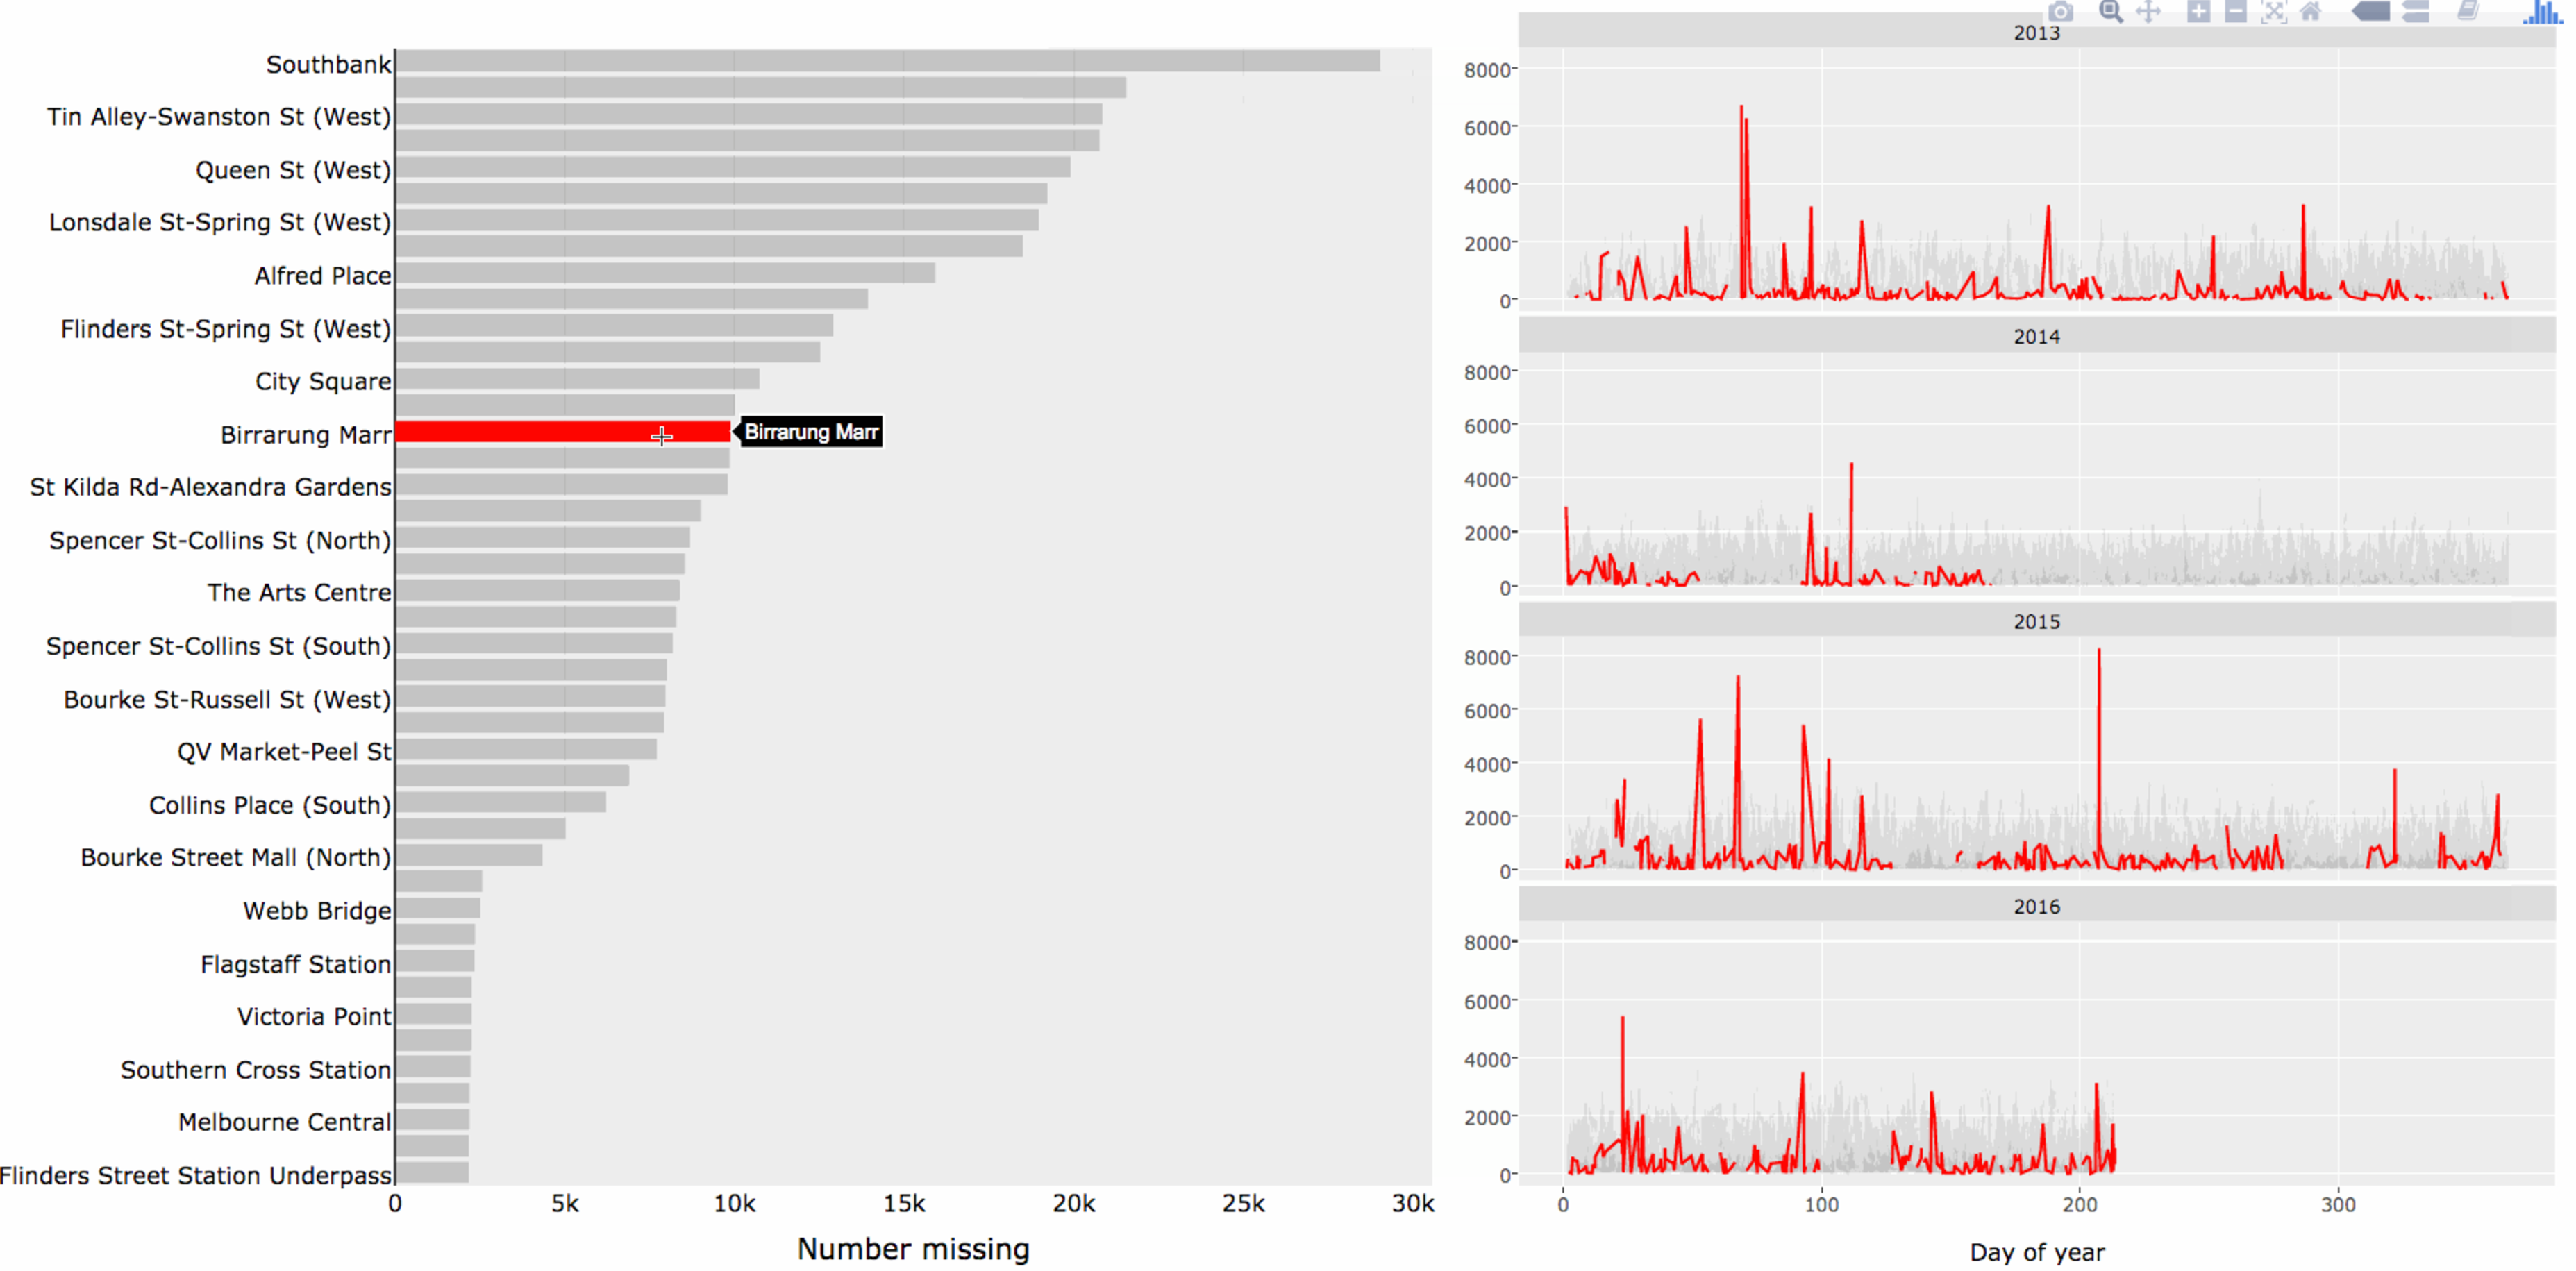
\includegraphics{images/pedestrians-missing.pdf}
\caption{\label{fig:missing-by-time}An interactive bar chart of the number
of missing counts by station linked to a sampled time series of counts.
See \href{https://vimeo.com/189035350}{here} for the corresponding video
and \href{http://cpsievert.github.io/pedestrians/missing-by-time/}{here}
for the interactive figure.}
\end{figure}

\subsubsection{Exploring trend and
seasonality}\label{exploring-trend-and-seasonality}

A time series \(Y_t\) can be thought of as a linear combination of at
least three components:

\[Y_t = T_t + S_t + I_t, \hspace{0.4cm} t \in \{1, \dots, T \} \] where
\(T_t\) is the trend, \(S_t\) is the seasonality, and \(I_t\) is the
``irregular'' component (i.e., remainder). For the sensor data, we could
imagine having multiple types of seasonality (e.g., hour, day, month,
year), but as Figure \ref{fig:missing-by-time} showed, year doesn't seem
to have much effect, and as we will see later, hour of day has a
significant effect (which is sensible for most traffic data), so we
focus on hour of day as a seasonal component. Estimating these
components has important applications in time series modeling (e.g.,
seasonal adjustments), but we could also leverage these estimates to
produce further time series ``features'' to guide our graphical
analysis.

There are many to go about modeling and estimating these time series
components. Partly due to its widespread availability in R, the
\texttt{stl()} function, which is based on LOESS smoothing, is a popular
and reasonable approach (R. B. Cleveland and Terpenning
\protect\hyperlink{ref-stl}{1990}); (R Core Team
\protect\hyperlink{ref-RCore}{2015}). Both the \textbf{anomalous} and
\textbf{tscognostics} R packages use estimates from
\texttt{stl()}\footnote{If no seasonal component exists, a Generalized
  Additive Models is used to estimate the trend component (Wood
  \protect\hyperlink{ref-mgcv}{2006}).} to measure the strength of trend
(as \(\hat{Var(T_t)}\)) and strength of seasonality (as
\(\hat{Var(S_t)}\)) (Hyndman, Wang, and Laptev
\protect\hyperlink{ref-anomalous}{2016}); (Wang
\protect\hyperlink{ref-tscognostics}{2016}). From these estimates, they
produce other informative summary statistics, such as the seasonal peak
(\(Max_{t}(\hat{S_t})\)), trough (\(Min_{t}(\hat{S_t})\)), spike (
\(Var[(Y_t - \bar{Y})^2]\)); as well as trend linearity
(\(\hat{\beta_1}\)) and curvature (\(\hat{\beta_2}\)) (coefficients from
a 2nd degree polynomial fit to the estimated trend
\(\mu = \beta_0 + \beta_1\hat{T_t} + \beta_2\hat{T_t^2}\)).

After computing these 7 different summary statistics for each sensor, we
may graphically explore the 7-dimensional space that they live in, as
shown in Figure \ref{fig:pedestrians-stl-tour}. The top row of Figure
\ref{fig:pedestrians-stl-tour} shows different views of the summary
statistics: in the left-hand side is an animated display which
interpolates between random 2D projections of the 7 dimensions (aka, a
grand tour) and on the right-hand side is a parallel coordinates plot
(Asimov \protect\hyperlink{ref-grand-tour}{1985}). For the parallel
coordinates plot, each dimension is standardized to have mean 0 and
standard deviation 1. The parallel coordinates plot helps to reveal an
unusual station (Tin Alley-Swanson St) in terms of both curvature and
linearity, which is then highlighted so we can visually track the
unusual point as it lies in this 7 dimensional feature space.

The static image in Figure \ref{fig:pedestrians-stl-tour} captures the
state of the interactive graphic after Tin Alley-Swanson St has been
selected and highlighted in red. The same sampled counts behind Figure
\ref{fig:missing-by-time} are used to generate the scatterplot (count
versus hour of day) in the lower left-hand panel. The lower right-hand
panel displays the inter-quartile range (IQR) by hour for the entire
dataset. The black ribbon is the overall IQR and the red ribbon is the
IQR for Tin Alley-Swanson St.~Having both the IQR and the raw counts in
the same display is useful for gaining an understanding of the variation
in seasonality over time (IQR), while still being able to discover
outliers or unusual patterns (raw).

\begin{figure}
\centering
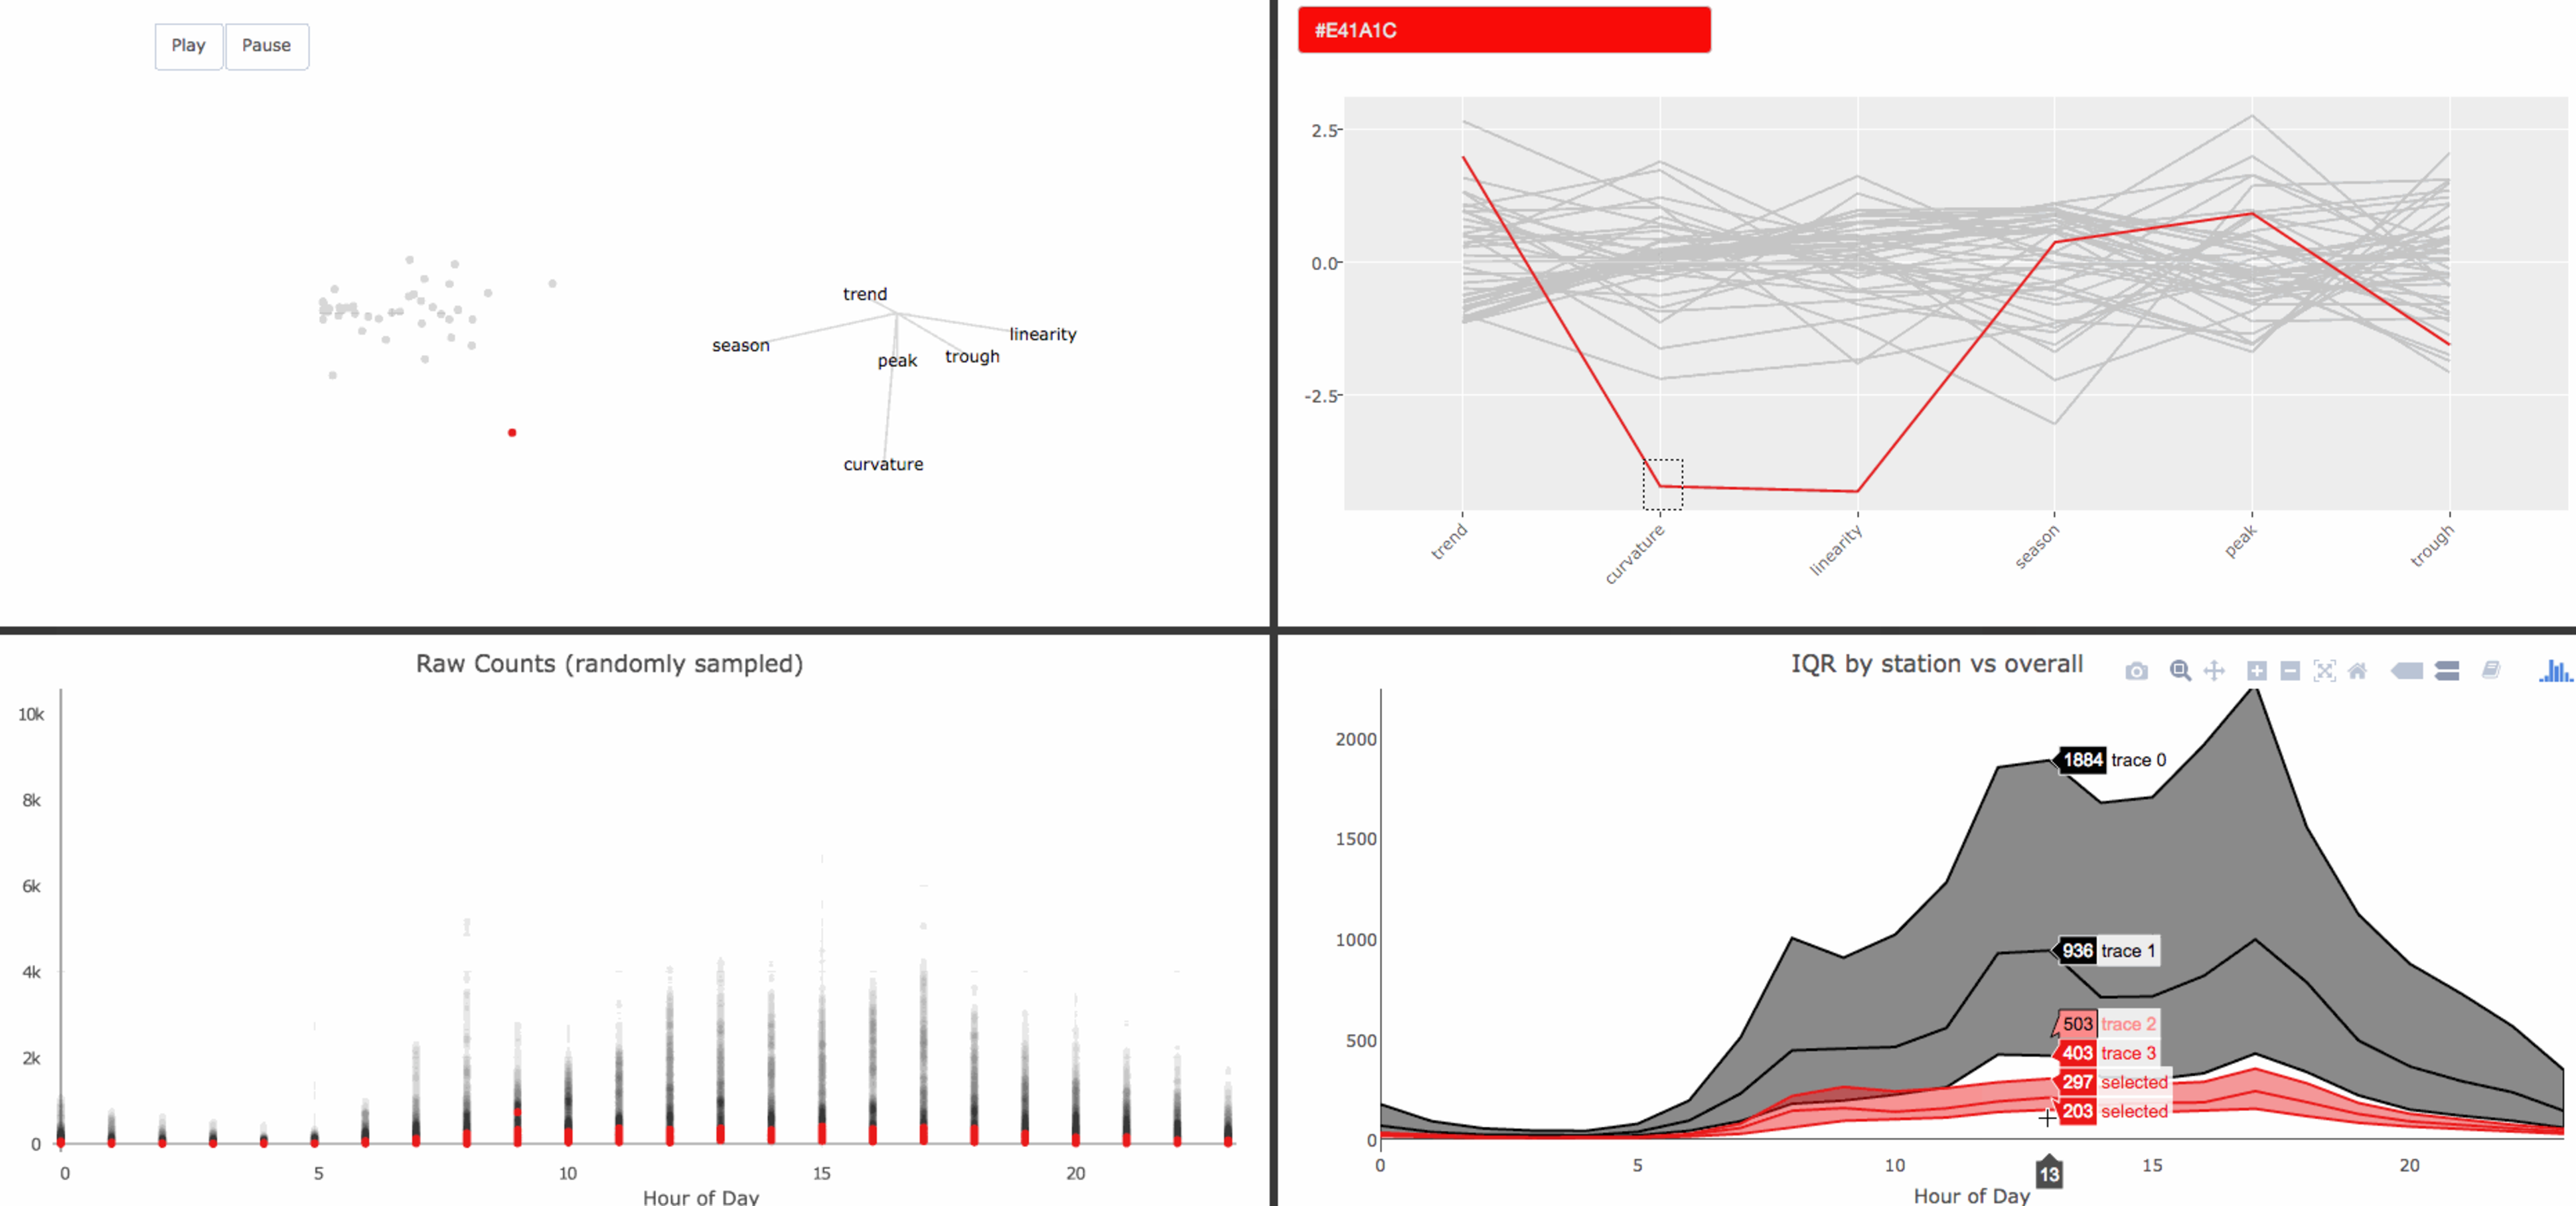
\includegraphics{images/pedestrians-stl-tour.pdf}
\caption{\label{fig:pedestrians-stl-tour}Linking views of counts (second
row) with features generated from seasonal trend decomposition (first
row). The top left panel shows a grand tour of the 7 dimensional space
and the top right panel a parallel coordinates plot. In both views, it
is apparent that one station (Tin Alley-Swanson St), highlighted in red,
has irregular curvature and linearity compared to the other stations. By
linking raw counts and the hourly IQR, we can see that this station
experiences relatively low traffic (red) compared to overall traffic
(black). See \href{https://vimeo.com/189170669}{here} for the
corresponding video and
\href{http://cpsievert.github.io/pedestrians/stl-tour/}{here} for the
interactive figure.}
\end{figure}

A careful inspection of the grand tour in Figure
\ref{fig:pedestrians-stl-tour} hints at another sensor that is
relatively close to Tin Alley-Swanson St in the feature space. Figure
\ref{fig:pedestrians-stl-tour2} uses a persistent linked brush to
highlight this other sensor (Bourke St-Russell St) in blue. Replaying
the tour (as shown in the video corresponding to Figure
\ref{fig:pedestrians-stl-tour2}) with these points highlighted different
colors makes it easier to track their distance (relative to each other
as well as the other points) throughout the feature space.

\begin{figure}
\centering
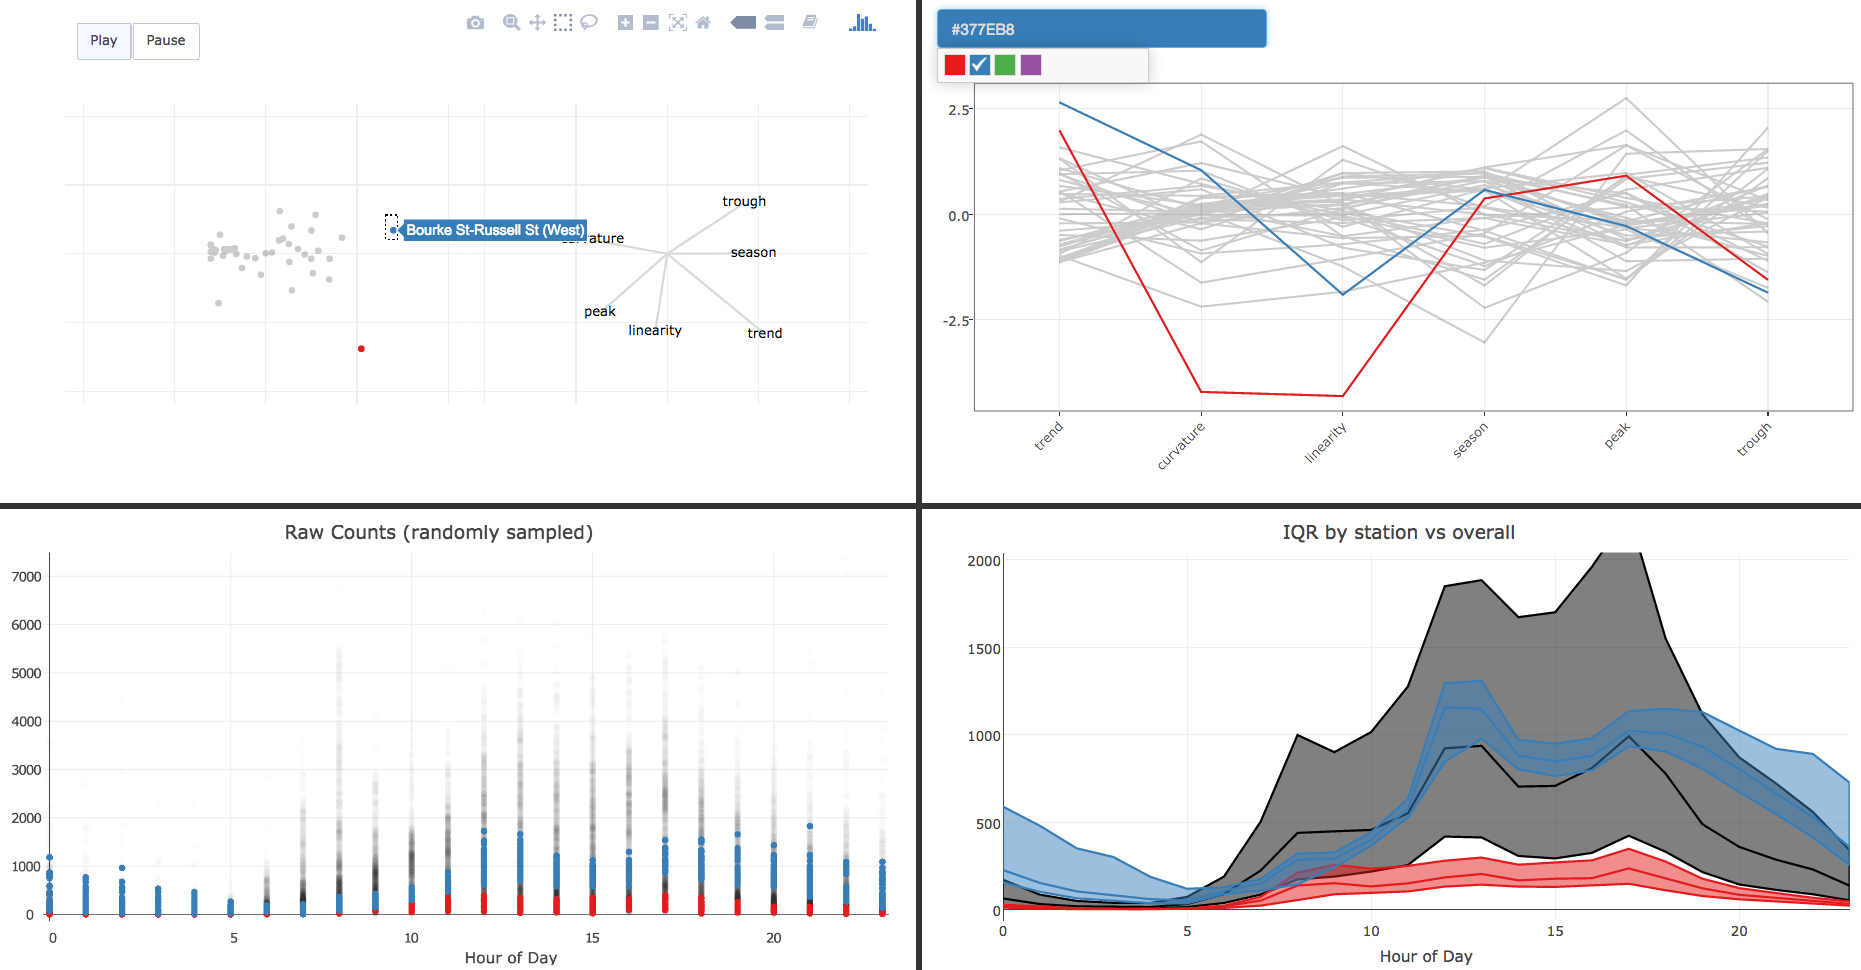
\includegraphics{images/pedestrians-stl-tour2}
\caption{\label{fig:pedestrians-stl-tour2}Using persistent linked brushing
to compare the trend and seasonality of Tin Alley-Swanson St.~to Bourke
St-Russell St (West). See \href{https://vimeo.com/189048529}{here} for
the corresponding video and
\href{http://cpsievert.github.io/pedestrians/stl-tour/}{here} for the
interactive figure.}
\end{figure}

A fair amount of insight can be extracted from the interactive graphic
in Figure \ref{fig:pedestrians-stl-tour}, but focusing just on the
STL-based features is somewhat limiting. There are certainly other
features that capture aspects of the time series that these features
have missed. In theory, the mathematics and the visualization techniques
behind Figure \ref{fig:pedestrians-stl-tour} can be extended to any
number of dimensions. In practice, technology and time typically limits
us to tens to hundreds of dimensions. The next section incorporates more
features and also links this information to a geographic map so we can
investigate the relationship between geographic location and certain
features.

\subsubsection{Exploring many features}\label{exploring-many-features}

Figure \ref{fig:pedestrians-cog-tour} is an extension of Figure
\ref{fig:pedestrians-stl-tour} to incorporate 10 other time series
features, as well as a map of Melbourne. In this much larger feature
space, Tin Alley-Swanson St. (highlighted in red) is still an unusual
sensor, but not quite as unusual as Waterfront City (highlighted in
blue). Also, rather interestingly, both of these sensors are located on
the outskirts of the city, relative to the other sensors. It appears
Waterfront City is so noticeably unusual due to its very large value of
lumpiness (defined as the variance of block variances of size 24).
Inspecting the unusually high raw counts for this station reveals some
insight as to why that is case -- the counts are relatively low
year-round, but then spike dramatically on new years eve and on January
26th. A Google search reveals that Waterfront City is a popular place to
watch fireworks. This is a nice example of how interactive graphics can
help us discover and explain \emph{why} unusual patterns occur.

\begin{figure}
\centering
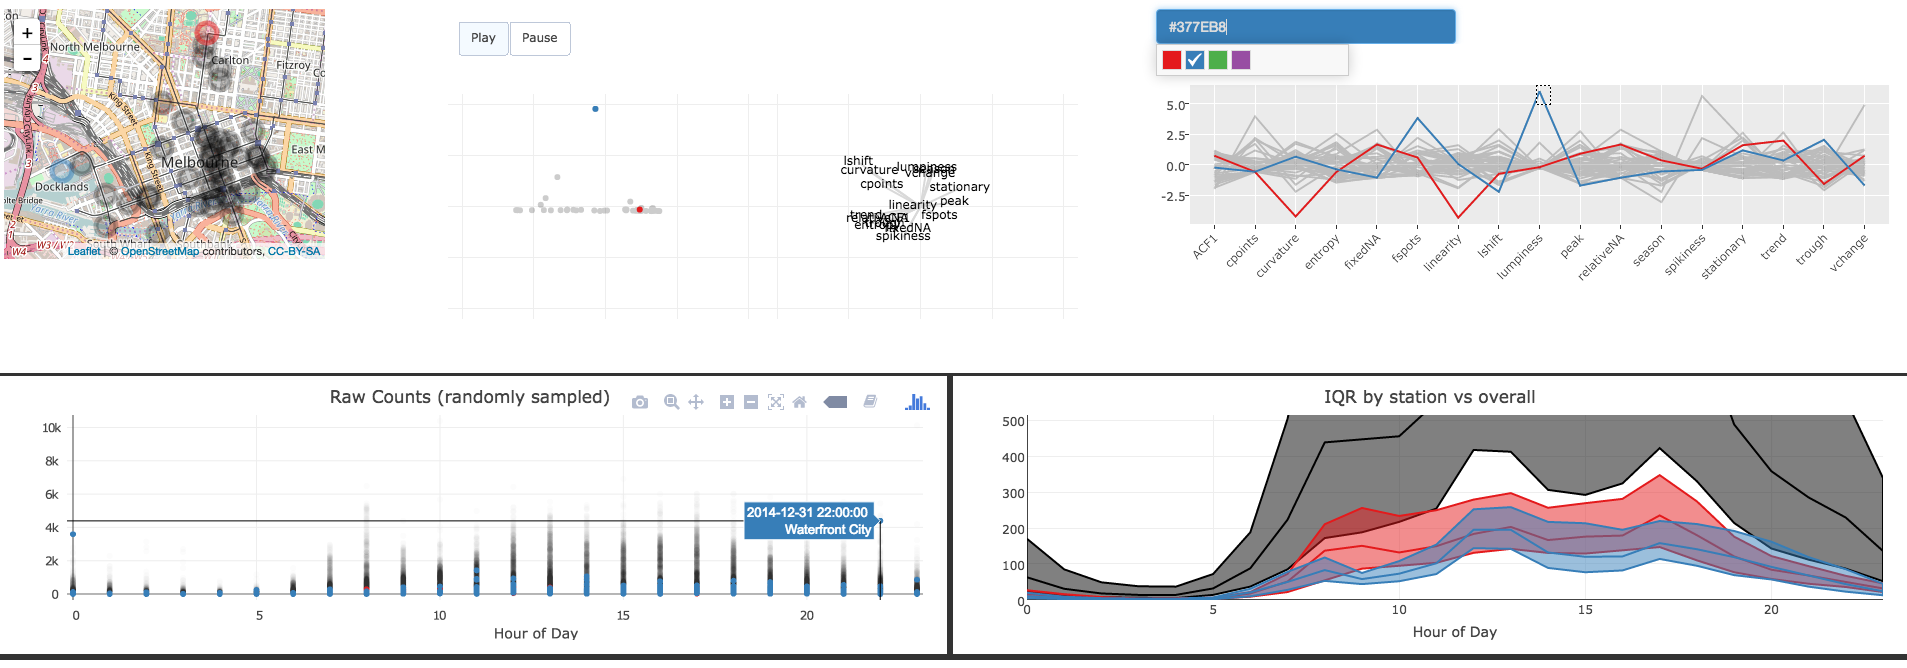
\includegraphics{images/pedestrians-cog-tour}
\caption{\label{fig:pedestrians-cog-tour}Seventeen time series features
linked to a geographic map as well as raw counts. This static image was
generated using a persistent brush to compare Tin Alley-Swanson St. (in
red) to Waterfront City (in blue). In addition to being unusual in the
feature space, these sensors are also on the outskirts of the city. See
\href{https://vimeo.com/189185214}{here} for the corresponding video and
\href{http://cpsievert.github.io/pedestrians/cog-tour/}{here} for the
interactive figure.}
\end{figure}

In addition to discovering interesting details, we can also use Figure
\ref{fig:pedestrians-cog-tour} to make meaningful comparisons in overall
behavior across numerous sensors. Figure
\ref{fig:pedestrians-cog-tour-acf} uses a persistent linked brush to
compare sensors with a high first order autocorrelation
(\(Corr(Y_t, Y_{t-1})\)), in red, against sensors with low
autocorrelation, in blue. A few interesting observations can be made
from this selection state.

\begin{figure}
\centering
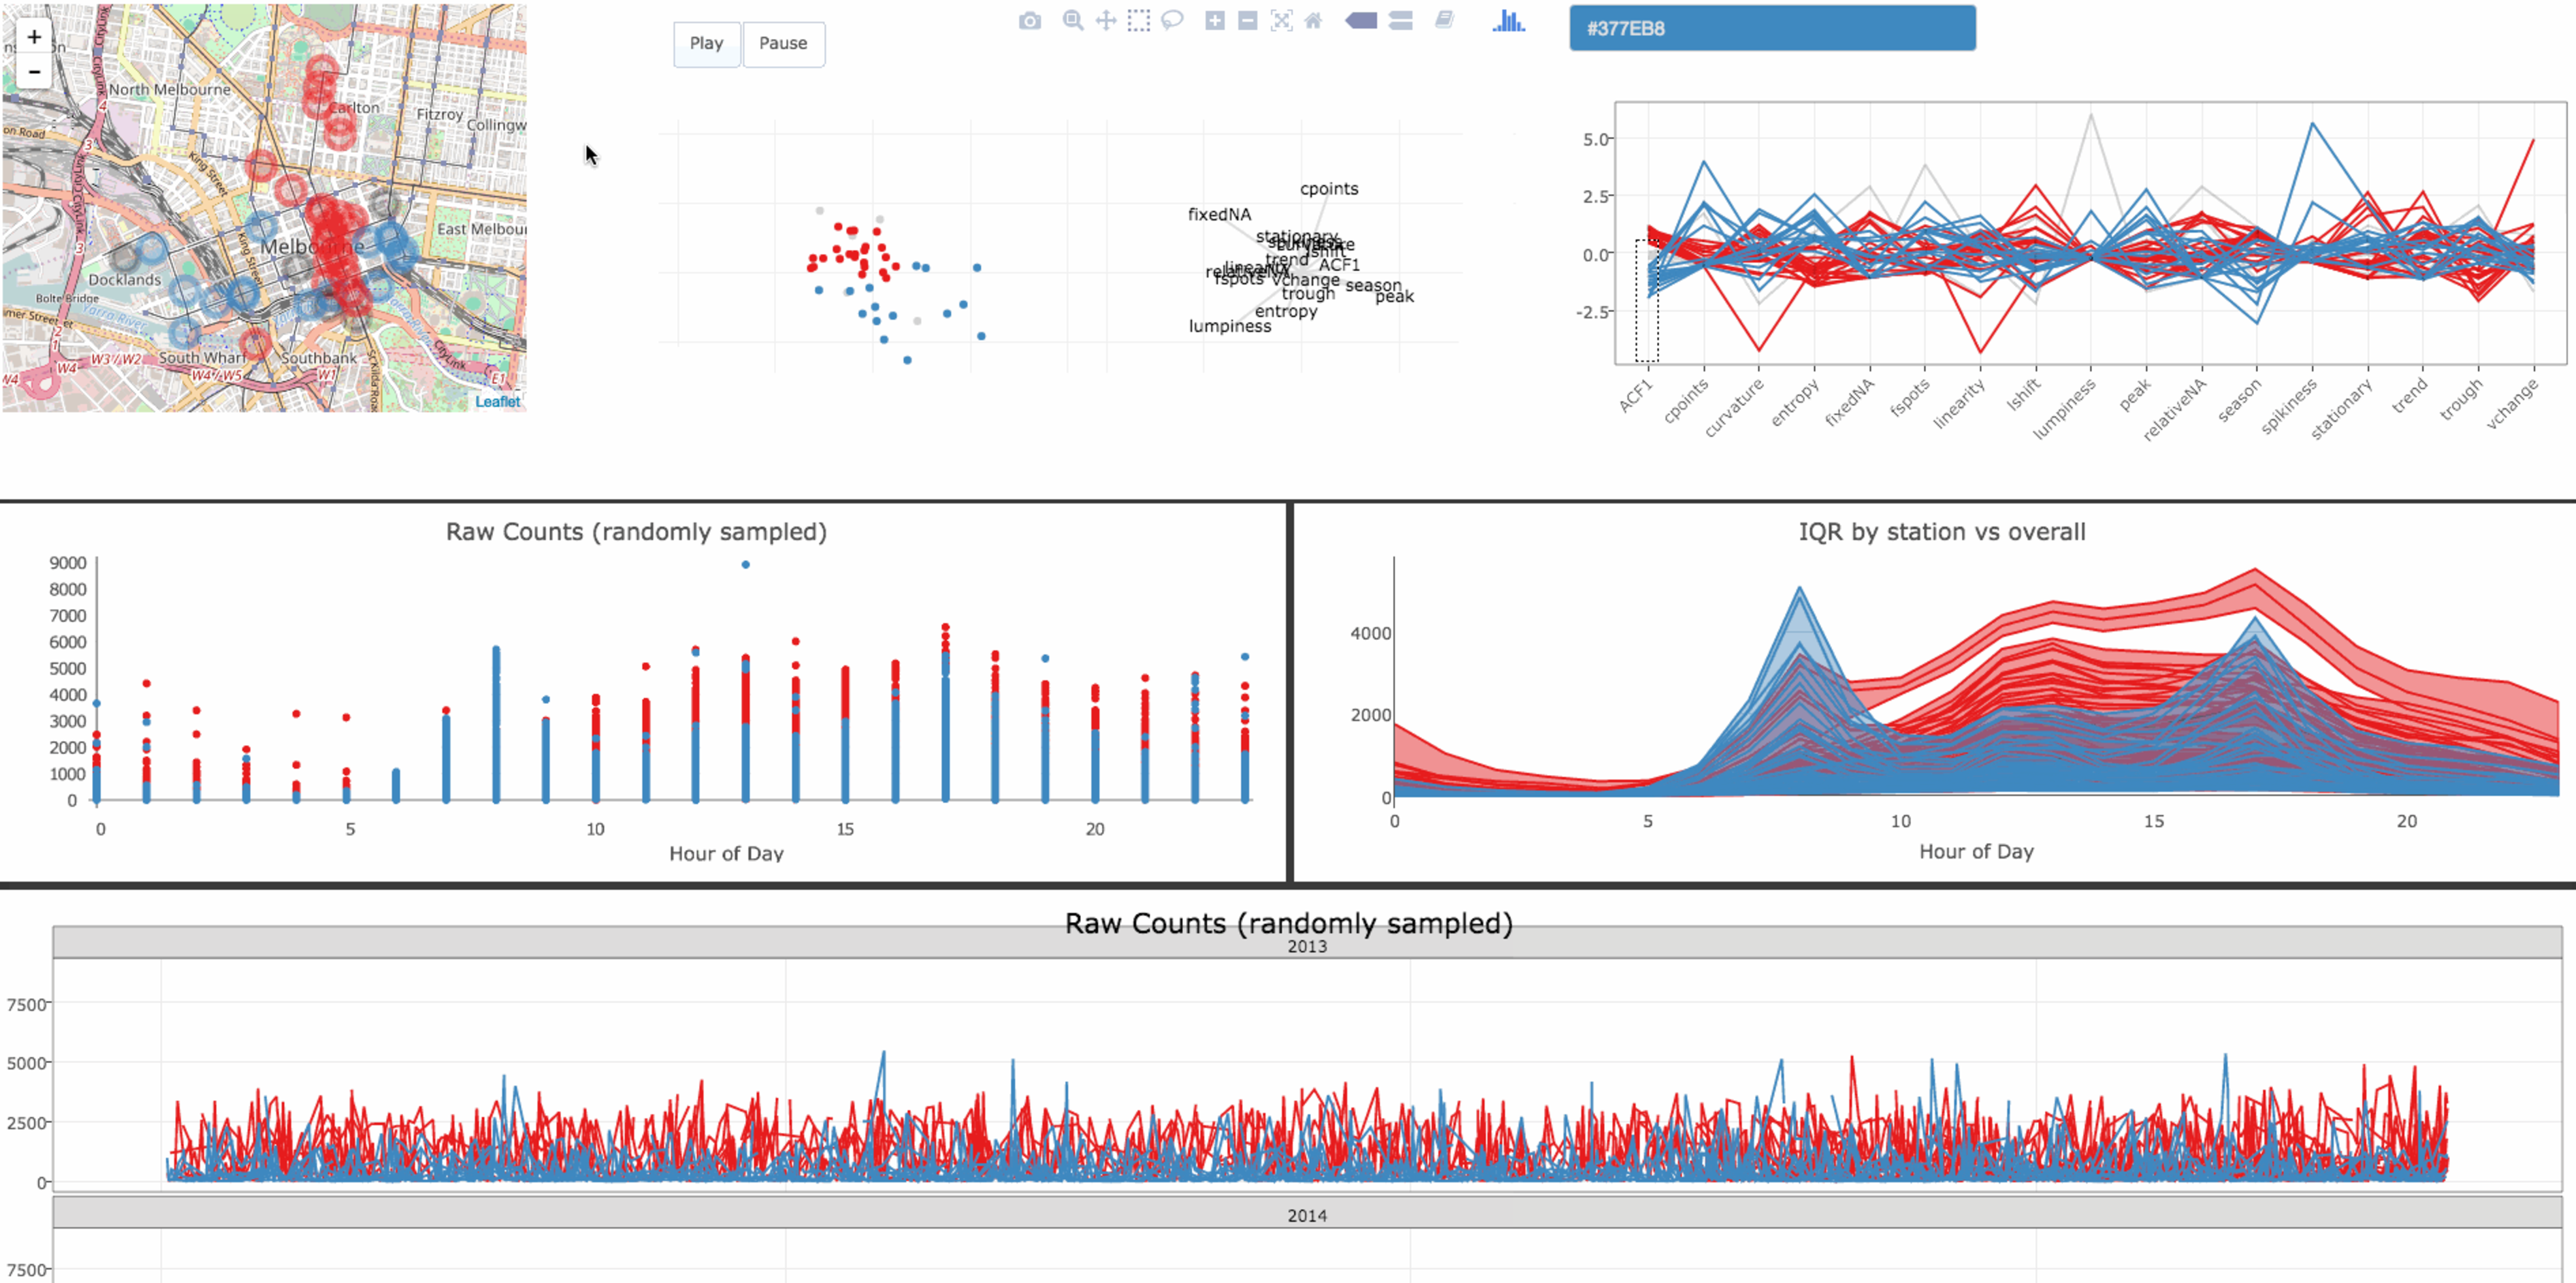
\includegraphics{images/pedestrians-cog-tour-acf.pdf}
\caption{\label{fig:pedestrians-cog-tour-acf}Sensors with high first order
autocorrelation (in red) versus sensors with low autocorrelation (in
blue). See \href{https://vimeo.com/189187319}{here} for the
corresponding video and
\href{http://cpsievert.github.io/pedestrians/cog-tour/}{here} for the
interactive figure.}
\end{figure}

The most striking relationship with respect to autocorrelation in Figure
\ref{fig:pedestrians-cog-tour-acf} is in the geographic locations.
Sensors with high autocorrelation (red) appear along Swanson St. -- the
heart of the central business district in Melbourne. These stations
experience a fairly steady flow of traffic throughout the day since both
tourists and people going to/from work use nearby trains/trams to get
from place to place. On the other hand, sensors with a low
autocorrelation\footnote{It should be noted that the (raw)
  autocorrelation is positive for each station with a minimum of 0.66,
  median of 0.83, and max of 0.94.} see the bulk of their traffic at the
start and end of the work day. It seems that this feature alone would
provide a fairly good criteria for splitting these sensors into 2
groups, which we could verify and study further via hierarchical
clustering.

Figure \ref{fig:pedestrians-dendro} links a dendrogram of a hierarchical
cluster analysis (using the complete linkage method via the
\texttt{hclust()} function in R) to other views of the data. A
persistent brush selects all the sensors under a given node --
effectively providing a tool to choose a number of clusters and
visualize model results in the data space (in real-time). Splitting the
dendrogram at the root node splits the sensors into 2 groups (red and
green) which confirms prior suspicions -- sensors on Swanson St (high
autocorrelation) are most different from sensors on the outskirts of the
city (low autocorrelation). Increasing the number of clusters to 3-4
splits off the unusual sensors that we identified in our previous
observations (Waterfront City, Birrarung Marr, and Tin Alley-Swanson
St).

\begin{figure}
\centering
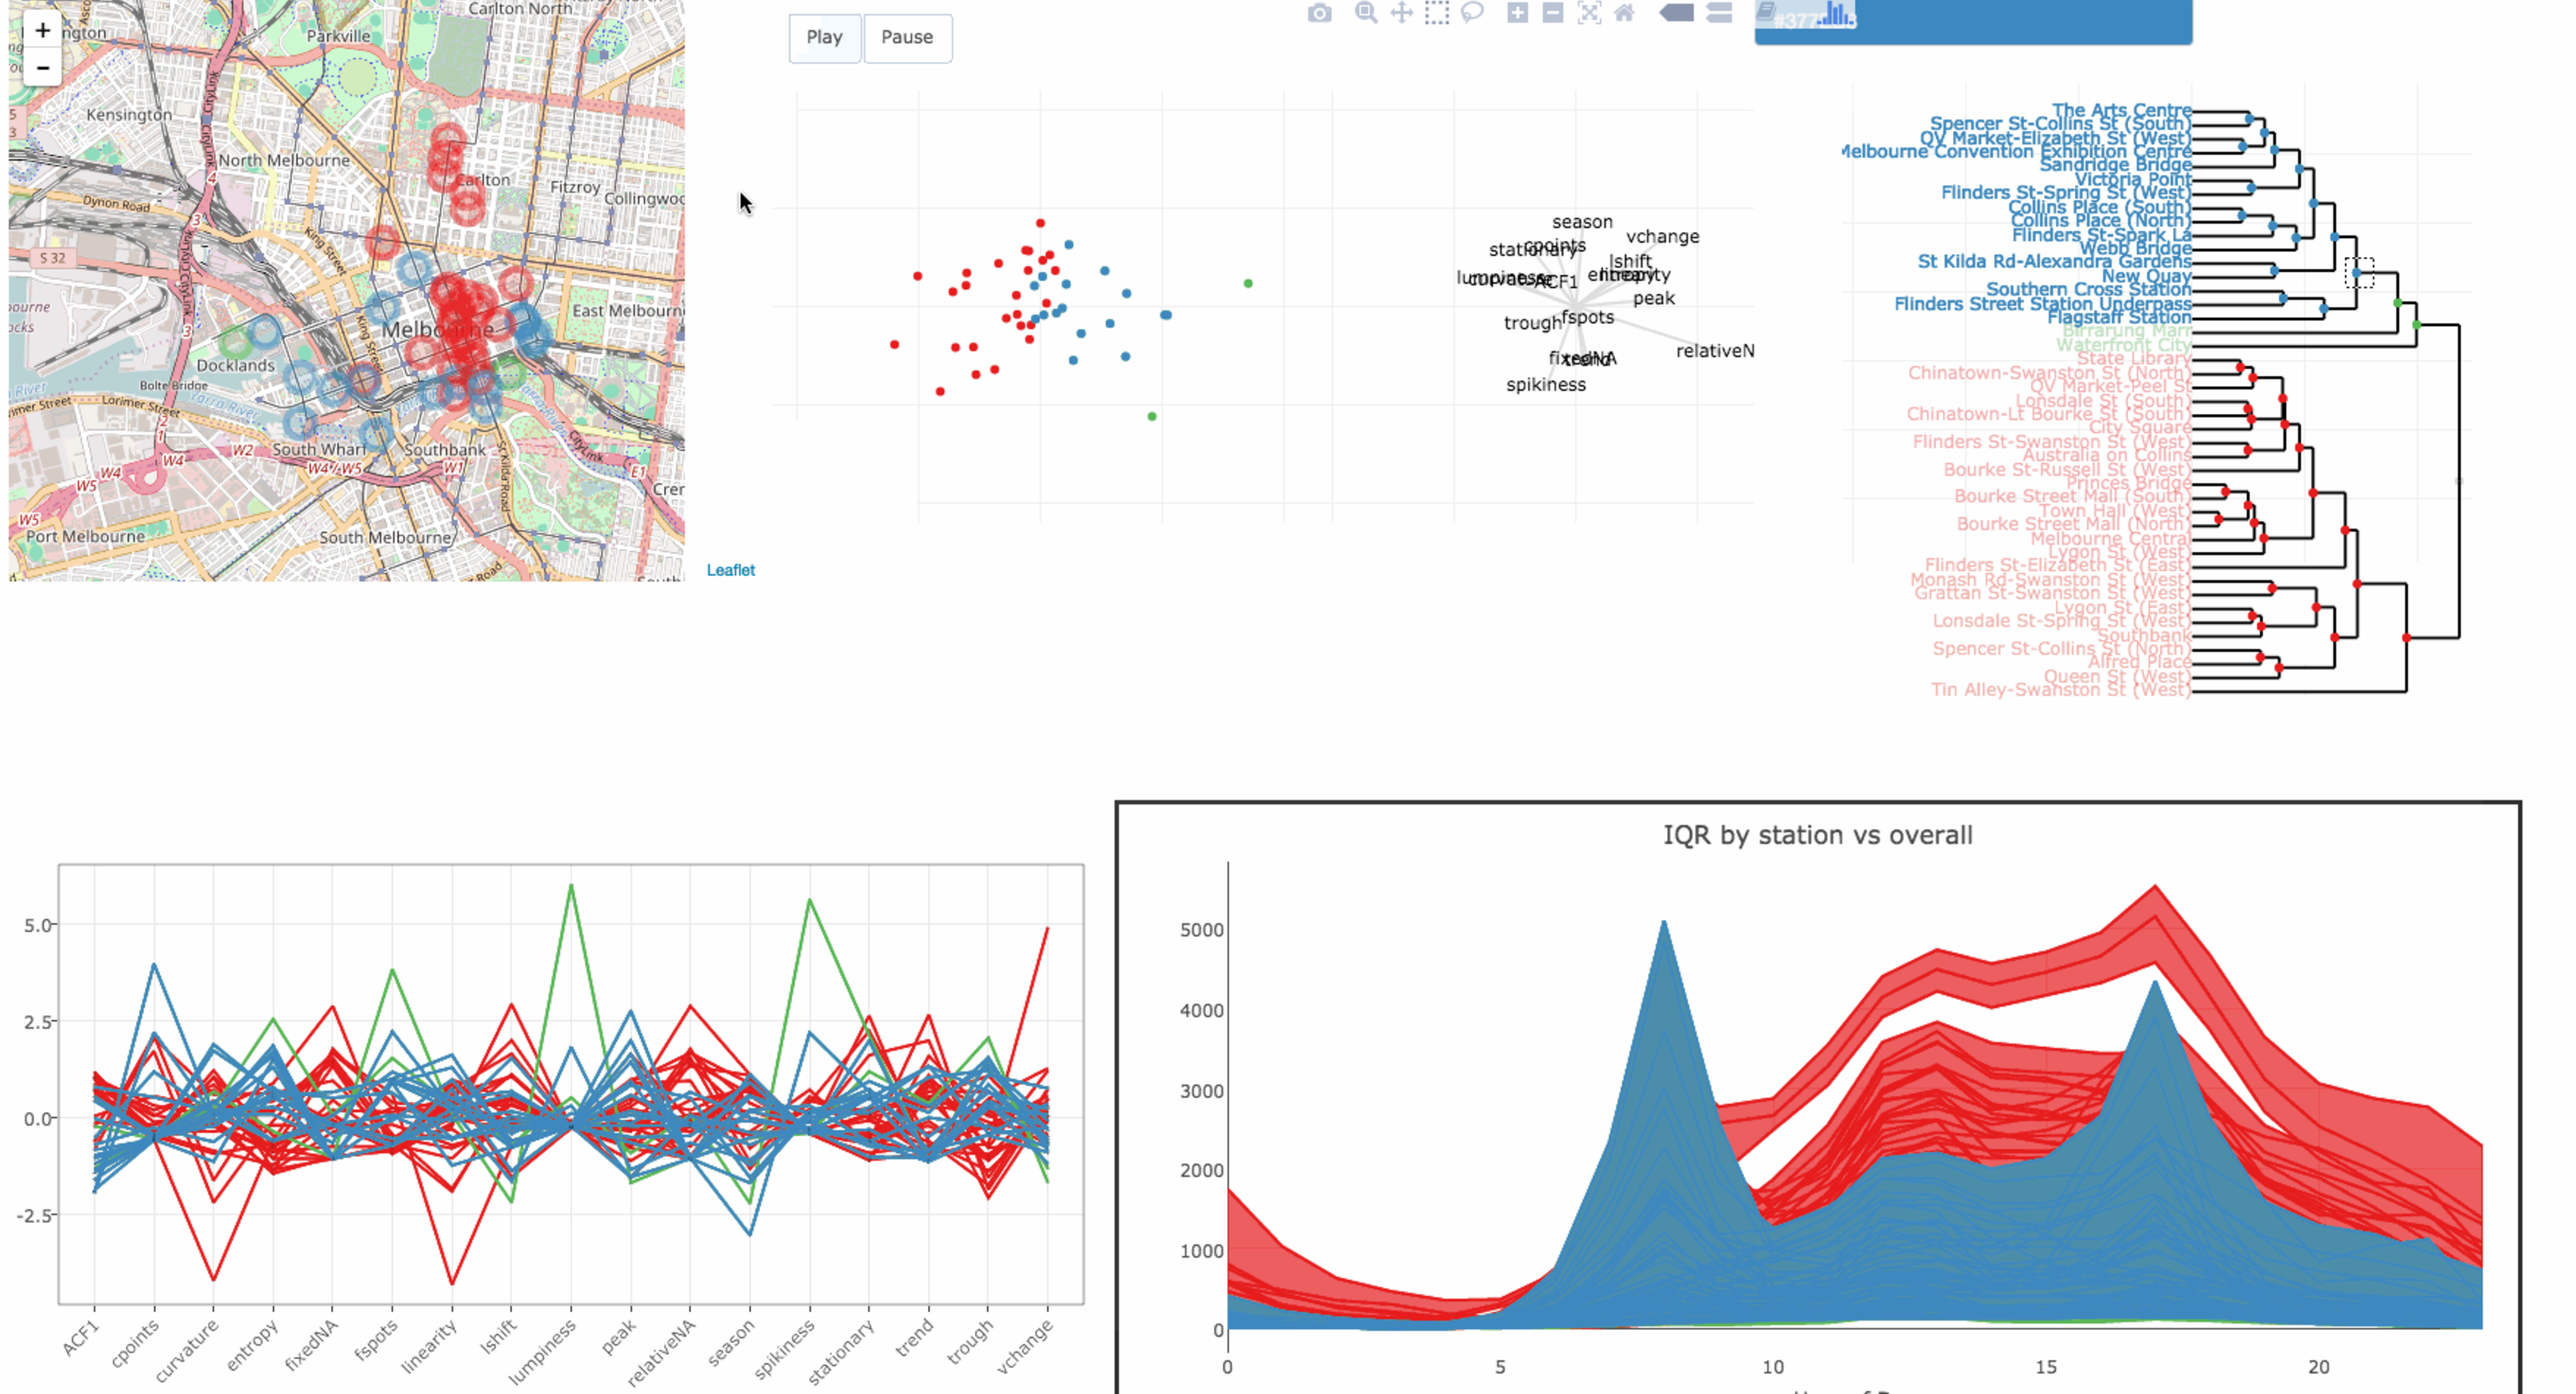
\includegraphics{images/pedestrians-dendro.pdf}
\caption{\label{fig:pedestrians-dendro}Linking a dendrogram of hierarchical
clustering results to multiple views of the raw data. See
\href{https://vimeo.com/189670650}{here} for the corresponding video and
\href{http://cpsievert.github.io/pedestrians/tour-dendro/}{here} for the
interactive figure.}
\end{figure}

This case study on pedestrian counts uses interactive graphic techniques
for numerous data analysis tasks. In fact, Figure
\ref{fig:pedestrians-cog-tour} alone provides at least one example of
each task outlined by Cook, Buja, and Swayne
(\protect\hyperlink{ref-Cook:2007uk}{2007}): finding Gestalt, posing
queries, and making comparisons. Furthermore, as Figure
\ref{fig:pedestrians-cog-tour} shows, and Wickham, Cook, and Hofmann
(\protect\hyperlink{ref-model-vis-paper}{2015}\protect\hyperlink{ref-model-vis-paper}{b})
writes, these same interactive techniques can also be a helpful for
understanding, inspecting, and diagnosing statistics models. The next
case study on Zika virus infections demonstrates how interactive
graphics can be useful for tracking disease outbreak and detecting data
quality issues.

\subsection{Tracking disease outbreak}\label{tracking-disease-outbreak}

The next case study investigates Zika disease outbreaks across North,
Central, and South America. The data was obtained from a publically
available repository that curates data from numerous public reports
across numerous countries and regions (Rodriguez et al.
\protect\hyperlink{ref-zika-data}{2016}). Of course, each country has a
different reporting method, so reported cases can and do fall under many
different categories. Thankfully, Rodriguez et al.
(\protect\hyperlink{ref-zika-data}{2016}) have done the tedious work of
standardizing these codes so we can combine all of these reports into a
single dataset. In some countries, reports are broken down to by
different demographics, and include reports of similar diseases such as
Flavi virus and GBS, but this analysis focuses specifically on
suspected/confirmed Zika cases at the location level.

The R package \textbf{zikar} bundles suspected/confirmed Zika cases at
the location level and provides specially designed tools for visualizing
it (Sievert
\protect\hyperlink{ref-zikar}{2016}\protect\hyperlink{ref-zikar}{c}).
All the graphics in this section were generated via the
\texttt{explore()} function from \textbf{zikar}, which invokes a
\textbf{shiny} app with linked interactive graphics (Chang et al.
\protect\hyperlink{ref-shiny}{2015}).\footnote{A hosted version of this
  web application is avaliable
  \href{http://104.131.111.111:3838/zikar/}{here}.} Figure
\ref{fig:zikar} displays the default view of the web application, which
provides a concise overview of the reported counts. The map on the
left-hand side shows the different reporting locations. The non-black
markers represent multiple locations, and hovering over a marker reveals
the entire region that the marker represents. From this, we can see that
the bulk of reporting locations are in the northern part of South
America and the southern part of Central America. The right hand side of
Figure \ref{fig:zikar} shows the overall density of weekly cases (on a
log scale) as well as the weekly median over time.

\begin{figure}
\centering
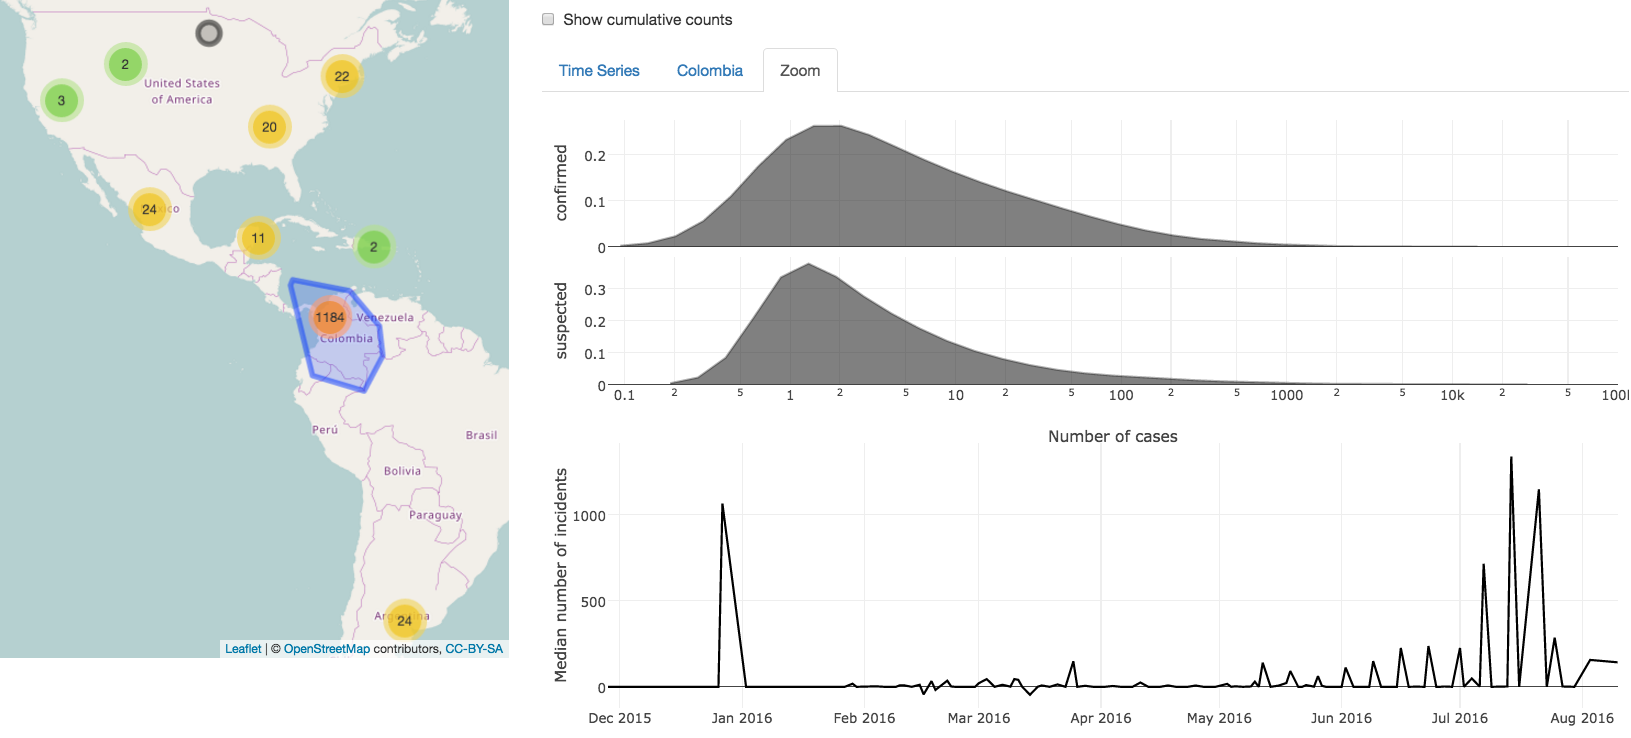
\includegraphics{images/zikar}
\caption{\label{fig:zikar}Multiple views of the Zika outbreak data. On the
left-hand side is a map of the reporting locations. On the right is the
overall density of suspected/confirmed cases reported per week (on a log
scale), and the overall weekly median over time.}
\end{figure}

Zooming and panning to a particular region on the interactive map
reveals more information conditioned on the bounding box of the map.
Figure \ref{fig:zikar-zoom} displays information specific to the
Dominican Republic. In the map itself, the ``marker clusters'' have
updated for a more granular view of the number of locations reporting
within the area. In the other views, statistics conditional upon this
region (in red) are overlayed against overall statistics (in black) for
fast and easy comparison(s). Figure \ref{fig:zikar-zoom} shows the
density of suspected cases in the Dominican is much higher than the
overall density, and the density for confirmed cases has a much larger
amount of variation. Furthermore, the weekly median within this region
is consistently higher from March 2016 to July 2016.

\begin{figure}
\centering
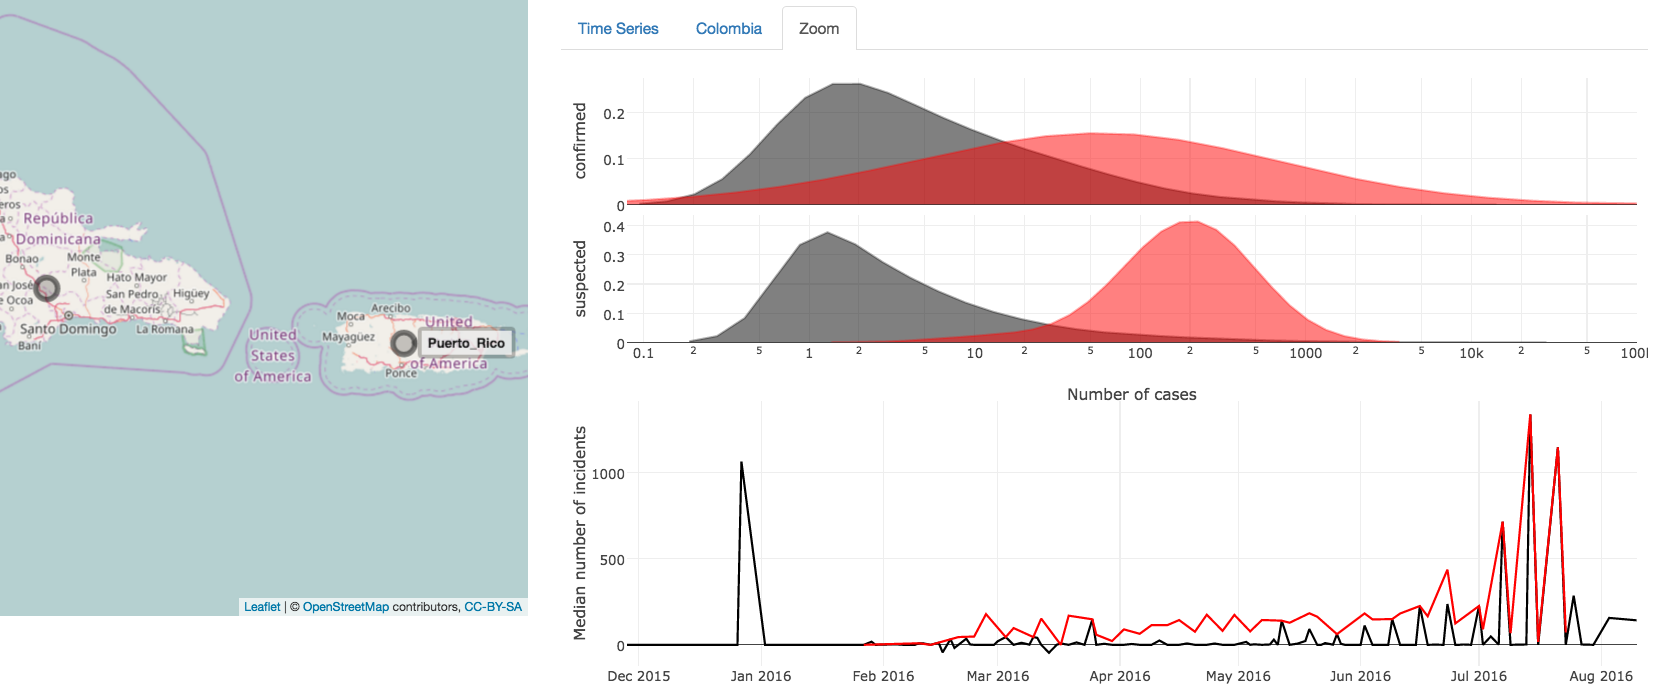
\includegraphics{images/zikar-zoom}
\caption{\label{fig:zikar-zoom}A comparison of the overall cases (in black)
to the cases conditional on the map bounds (in red). Zooming and panning
the interactive map dynamically updates the density estimates and median
number of incidents.}
\end{figure}

Figure \ref{fig:zikar} helps to point out an issue with the data -- in
some weeks, the median number of all reported cases is negative. Using
the zooming and panning capabilities of Figure \ref{fig:zikar}, one may
quickly find a sub-region of the map that reflects the same overall
issue, which helps to guide an investigation into why this issue exists.
Figure \ref{fig:zikar-nicaragua} uses this functionality to find that
both El Salvador and Nicaragua report negative counts, at different
times of the year. Considering that these countries report a cumulative
count of currently infected people, these negative non-cumulative counts
indicate mis-diagnosis or death. Since deaths caused by Zika in adults
are quite rare, and symptoms from the Zika virus are hard to
differentiate from the more common Dengue virus (another disease spread
via infected mosquitoes), mis-diagnosis seems to be the more likely
reason for the negative counts (Jr. and VICTOR
\protect\hyperlink{ref-zika-nyt}{2016}).

\begin{figure}
\centering
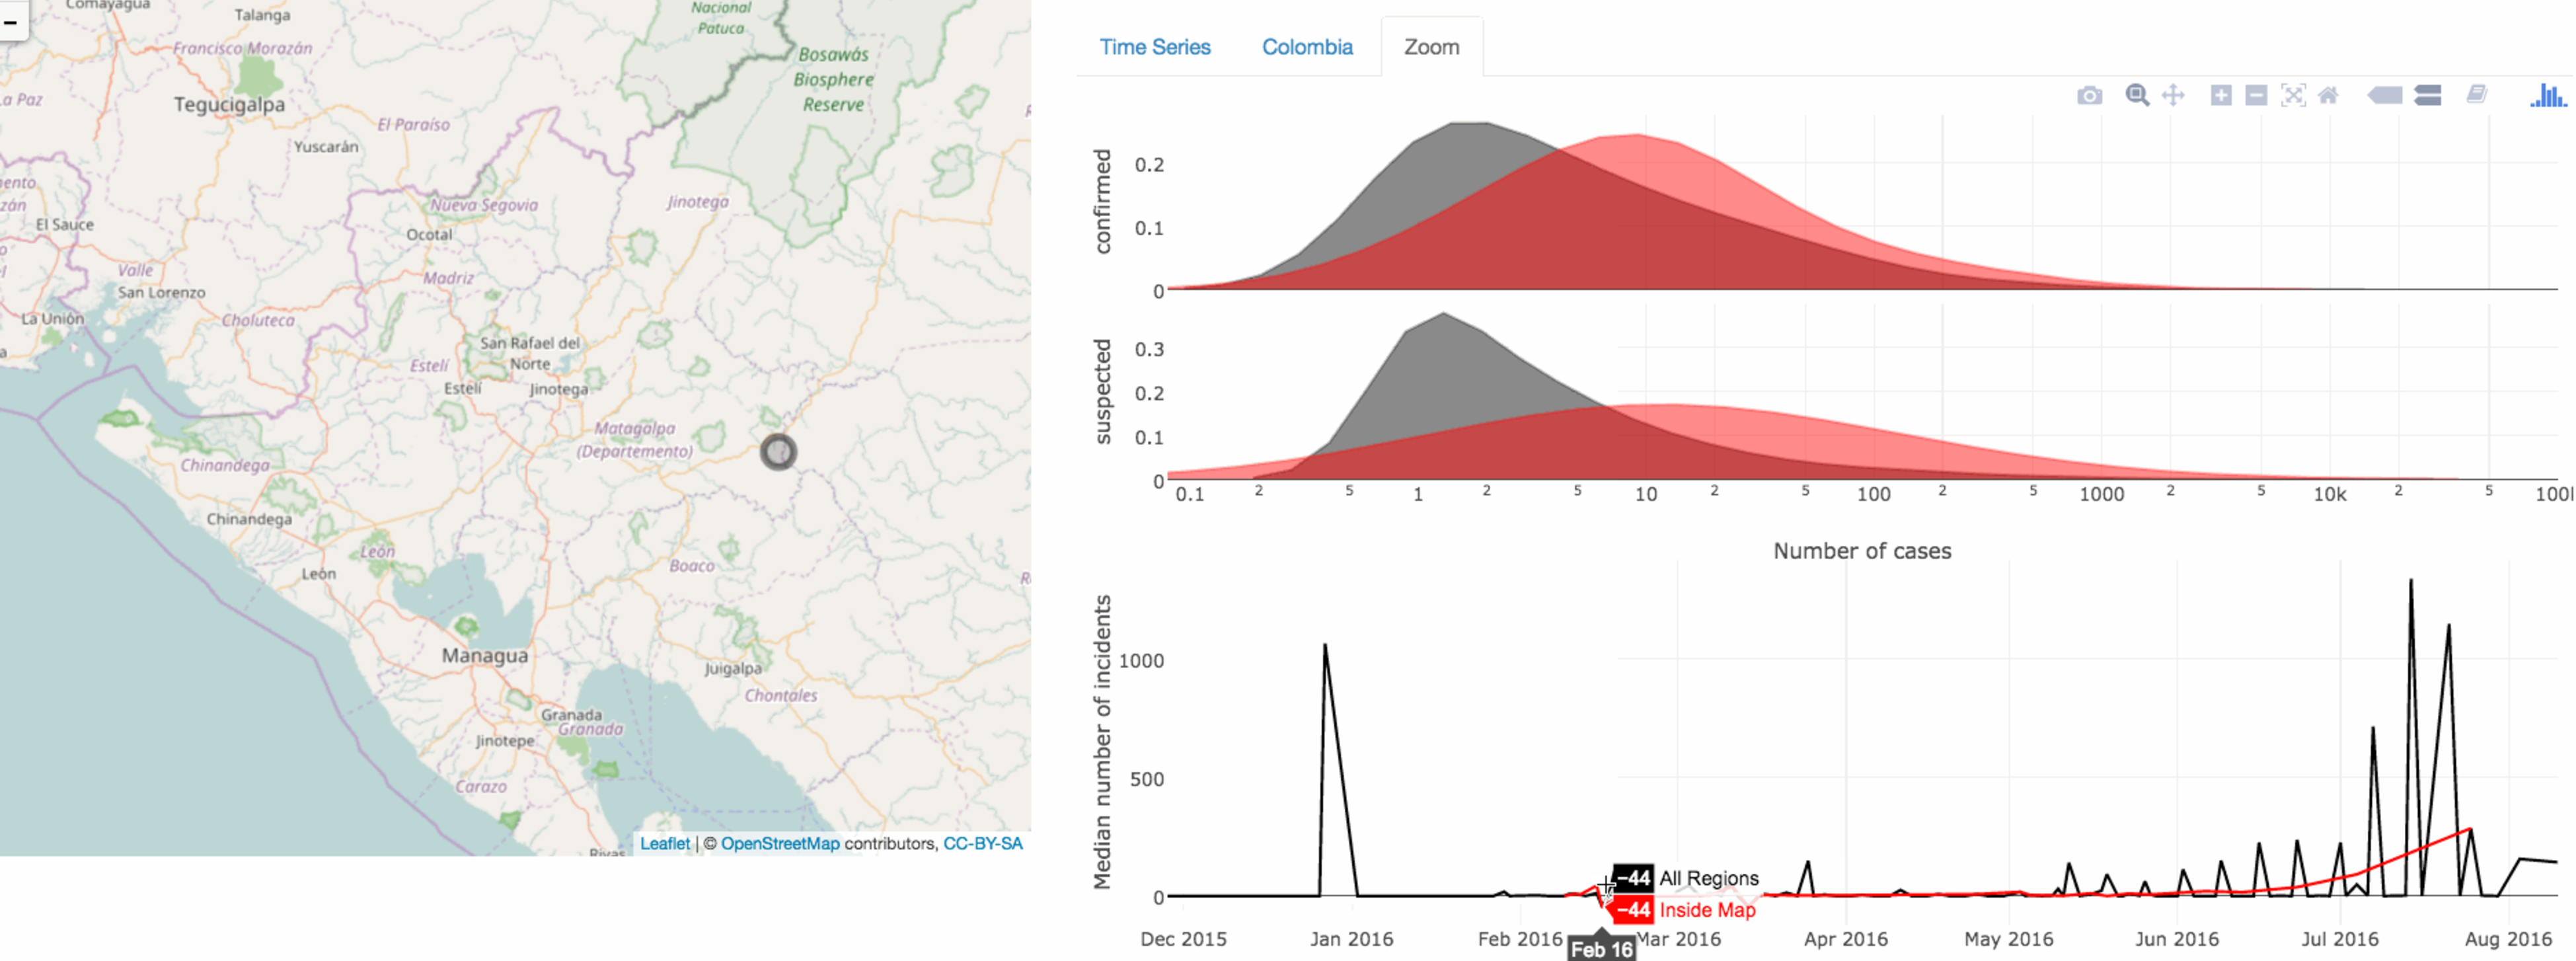
\includegraphics{images/zikar-nicaragua.pdf}
\caption{\label{fig:zikar-nicaragua}Zooming and panning to a region of the
map that has a negative median of overall cases (Nicaragua). A video of
the zooming and panning may be viewed
\href{https://vimeo.com/190610577}{here}.}
\end{figure}

As it turns out, Nicaragua and El Salvador are not the only countries
that have reported a lower cumulative count from one week to the next.
Figure \ref{fig:zikar-cumulative} shows cumulative confirmed (in red)
and suspected (in blue) counts by location within 9 different countries.
Argentina is another country that has clearly encountered mis-diagnosis
issues -- there is a consistent dip in counts across all locations
within the country on two particular dates in May 2016. Although Figure
\ref{fig:zikar-cumulative} covers almost all the countries in this data,
it only covers \textasciitilde{}5\% of all reporting locations. Columbia
alone accounts for \textasciitilde{}95\% of all locations found in this
data and has some unique reporting issues of its own.

\begin{figure}
\centering
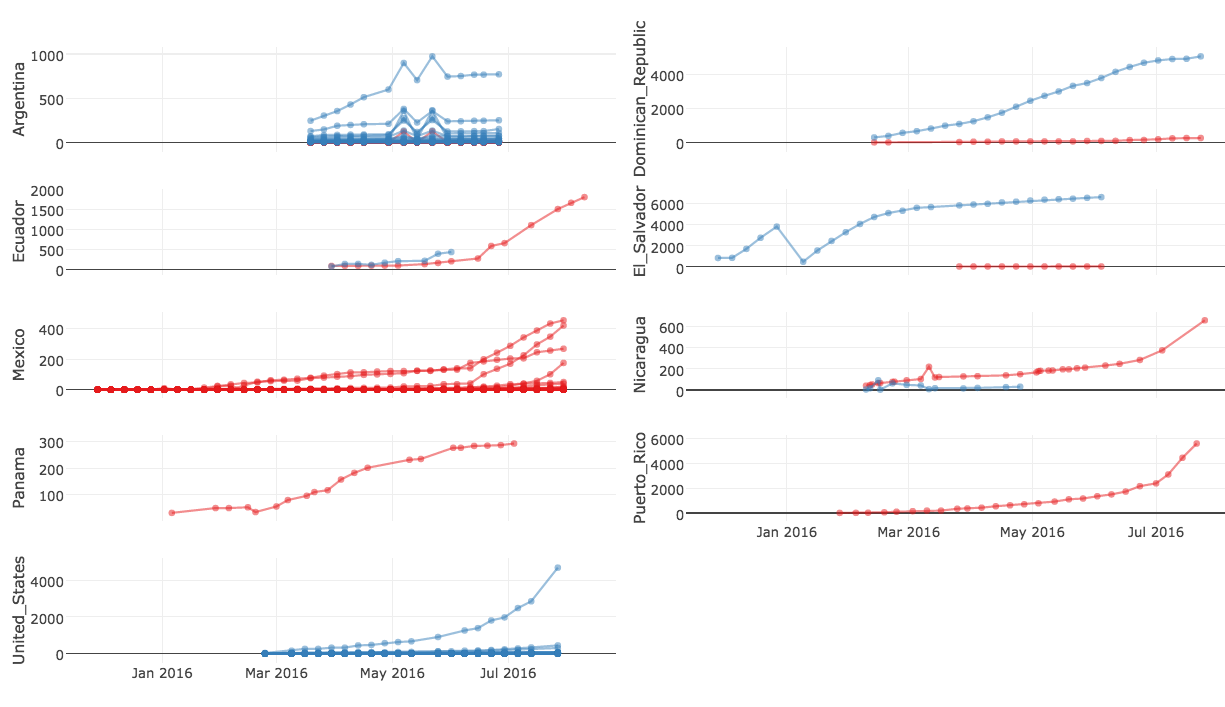
\includegraphics{images/zikar-cumulative}
\caption{\label{fig:zikar-cumulative}Cumulative confirmed (in red) and
suspected (in blue) counts by location within 9 different countries.}
\end{figure}

Figure \ref{fig:zikar-columbia} shows the cumulative number of confirmed
(in red) and suspected (in blue) cases for every reporting location in
Columbia. From the static version of Figure \ref{fig:zikar-columbia}, it
seems plausible that every location re-classified all confirmed cases to
suspected around mid-March. By clicking on a particular line (shown in
the video of Figure \ref{fig:zikar-columbia}) to highlight the
confirmed/suspected counts for a particular location, it becomes even
more obvious that every Columbian location simply changed all their
cases from confirmed to suspected.

\begin{figure}
\centering
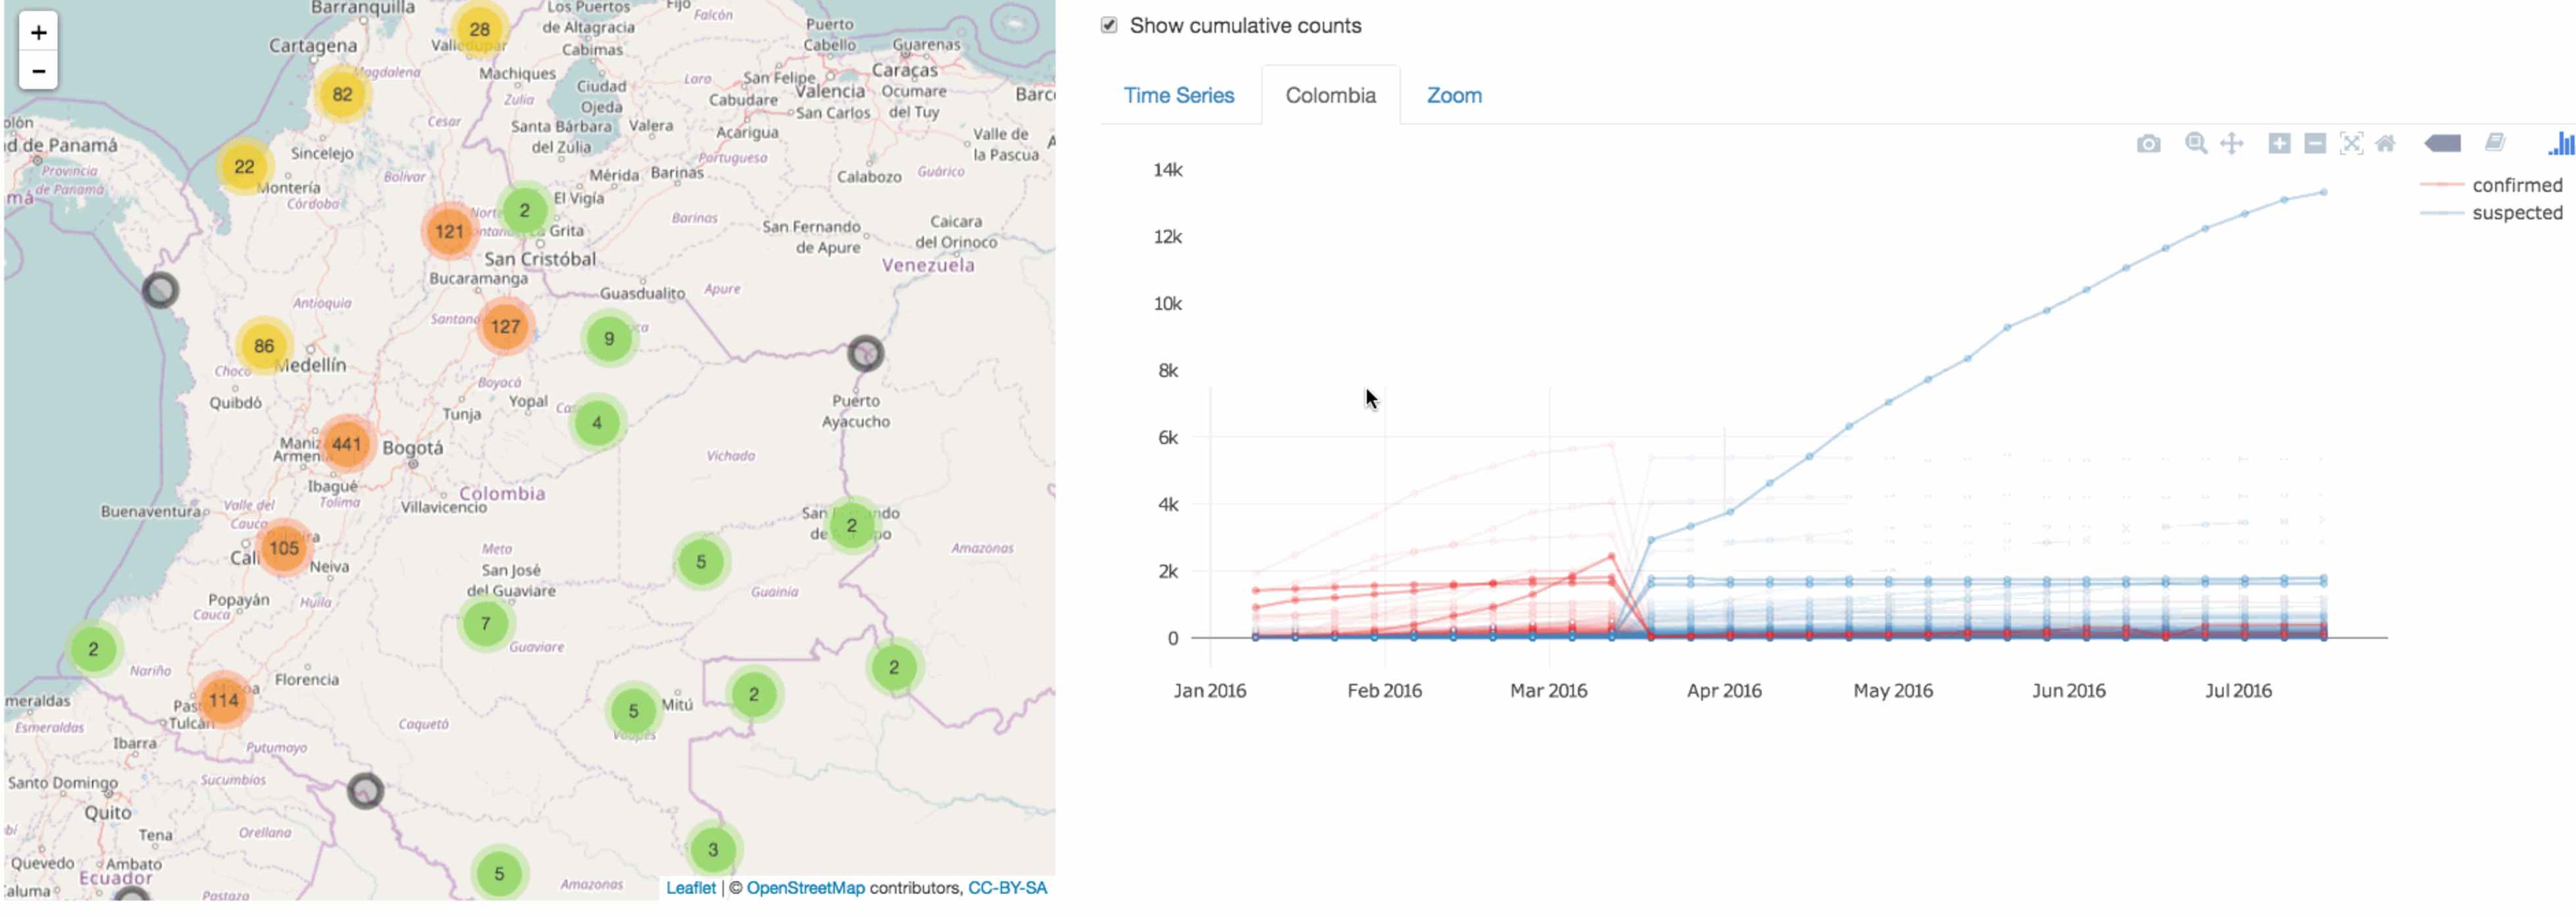
\includegraphics{images/zikar-colombia.pdf}
\caption{\label{fig:zikar-colombia}Highlighting cumulative confirmed (in
red) and suspected (in blue) counts by location within Colombia to
verify re-classifications from confirmed to suspected. A video of the
interactive highlighting may be viewed
\href{https://vimeo.com/190736801}{here}.}
\end{figure}

This case study shows how interactive graphics can be useful to discover
issues in data that should be addressed before any statistical modeling
occurs. For this reason, they are particularly useful for analysts
coming at the problem with a lack of domain expertise, and can provide
insight helpful for downstream analysis. The next case study uses
interactive graphics to explore Australian election data and provides a
nice example of combining numerous data sources into a single dashboard
of linked views.

\hypertarget{exploring-australian-election-data}{\subsection{Exploring
Australian election data}\label{exploring-australian-election-data}}

The next case study takes a look at the relationship between
demographics and voting behavior in the 2013 Australian federal
election. Demographic information was obtained from the Australian
Bureau of Statistics (ABS)\footnote{Downloaded from
  \url{https://www.censusdata.abs.gov.au/datapacks/}}, voting
information was obtained from the Australian Electoral Commission
(AEC)\footnote{Downloaded from
  \url{http://www.aec.gov.au/elections/federal_elections/2013/downloads.htm}},
and all the data and graphics presented here are available via the R
package \textbf{eechidna} (Cook et al.
\protect\hyperlink{ref-eechidna}{2016}). Thankfully, these data sources
are linked via electoral boundaries from the 2013 election (and the
geo-spatial boundaries are also available\footnote{\url{http://www.aec.gov.au/Electorates/gis/gis_datadownload.htm}}),
making it possible to explore the relationship between voting behavior
and demographics across electorates.

Figure \ref{fig:eechidna-2p}

\begin{figure}
\centering
\includegraphics{images/eechidna-2p.pdf}
\caption{\label{fig:eechidna-2p}Comparing demographics in electorate won by
the Liberal Party to the Labor Party.}
\end{figure}

\section{Conclusion}\label{conclusion-2}

\section{Acknowledgements}\label{acknowledgements-1}

Thank you to the organizers (Nicholas Tierney, Miles McBain, Jessie
Roberts) of the rOpenSci hackathon as well as my group members (Heike
Hofmann, Di Cook, Rob Hyndman, Ben Marwick, Earo Wang) where the
\textbf{eechidna} package first took flight. Thank you to Di Cook and
Earo Wang for sparking my interest in the pedestrians data, helping to
implement the \textbf{pedestrians} R package, and many fruitful
discussions (some with Heike Hofmann and Rob Hyndman).

\chapter{plotly for R}

This chapter contains many web-based interactive graphics and moving
images. Since moving images are not allowed on the University's
publishing platform, I highly suggest viewing the web-based version of
this chapter -- \url{https://cpsievert.github.io/plotly_book/}

\section{Two approaches, one object}\label{two-approaches-one-object}

There are two main ways to initiate a plotly object in R. The
\texttt{plot\_ly()} function transforms \emph{data} into a plotly
object, while the \texttt{ggplotly()} function transforms a \emph{ggplot
object} into a plotly object (Wickham
\protect\hyperlink{ref-ggplot2}{2009}\protect\hyperlink{ref-ggplot2}{a});
(Sievert et al. \protect\hyperlink{ref-plotly}{2016}). Regardless of how
a plotly object is created, printing it results in an interactive
web-based visualization with tooltips, zooming, and panning enabled by
default. The R package also has special semantics for
\protect\hyperlink{arranging-multiple-views}{arranging},
\protect\hyperlink{multiple-linked-views}{linking}, and
\protect\hyperlink{animating-views}{animating} plotly objects. This
chapter discusses some of the philosophy behind each approach, explores
some of their similarities, and explains why understanding both
approaches is extremely powerful.

The initial inspiration for the \texttt{plot\_ly()} function was to
support \href{https://github.com/plotly/plotly.js}{plotly.js} chart
types that \textbf{ggplot2} doesn't support, such as 3D surface and mesh
plots. Over time, this effort snowballed into an interface to the entire
plotly.js graphing library with additional abstractions inspired by the
grammar of graphics (Wilkinson
\protect\hyperlink{ref-Wilkinson:2005}{2005}). This newer
``non-ggplot2'' interface to plotly.js is currently not, and may never
be, as fully featured as \textbf{ggplot2}. Since we can already
translate a fairly large amount of ggplot objects to plotly objects, I'd
rather not reinvent those same abstractions, and advance our ability to
\protect\hyperlink{multiple-linked-views}{link multiple views}.

The next section uses a case study to introduce some of the similarities
between \texttt{ggplotly()}/\texttt{plot\_ly()}, introduces the concept
of a \protect\hyperlink{the-data-plot-pipeline}{data-plot-pipeline}, and
also demonstrates how to \protect\hyperlink{extending-ggplotly}{extend
\texttt{ggplotly()}} with functions that can modify plotly objects.

\subsection{A case study of housing sales in
Texas}\label{a-case-study-of-housing-sales-in-texas}

The \textbf{plotly} package depends on \textbf{ggplot2} which bundles a
data set on monthly housing sales in Texan cities acquired from the
\href{http://recenter.tamu.edu/}{TAMU real estate center}. After the
loading the package, the data is ``lazily loaded'' into your session, so
you may reference it by name:

\begin{Shaded}
\begin{Highlighting}[]
\KeywordTok{library}\NormalTok{(plotly)}
\NormalTok{txhousing}
\CommentTok{#> # A tibble: 8,602 × 9}
\CommentTok{#>      city  year month sales   volume median listings inventory  date}
\CommentTok{#>     <chr> <int> <int> <dbl>    <dbl>  <dbl>    <dbl>     <dbl> <dbl>}
\CommentTok{#> 1 Abilene  2000     1    72  5380000  71400      701       6.3  2000}
\CommentTok{#> 2 Abilene  2000     2    98  6505000  58700      746       6.6  2000}
\CommentTok{#> 3 Abilene  2000     3   130  9285000  58100      784       6.8  2000}
\CommentTok{#> 4 Abilene  2000     4    98  9730000  68600      785       6.9  2000}
\CommentTok{#> 5 Abilene  2000     5   141 10590000  67300      794       6.8  2000}
\CommentTok{#> 6 Abilene  2000     6   156 13910000  66900      780       6.6  2000}
\CommentTok{#> # ... with 8,596 more rows}
\end{Highlighting}
\end{Shaded}

In attempt to understand house price behavior over time, we could plot
\texttt{date} on x, \texttt{median} on y, and group the lines connecting
these x/y pairs by \texttt{city}. Using \textbf{ggplot2}, we can
\emph{initiate} a ggplot object with the \texttt{ggplot()} function
which accepts a data frame and a mapping from data variables to visual
aesthetics. By just initiating the object, \textbf{ggplot2} won't know
how to geometrically represent the mapping until we add a layer to the
plot via one of \texttt{geom\_*()} (or \texttt{stat\_*()}) functions (in
this case, we want \texttt{geom\_line()}). In this case, it is also a
good idea to specify alpha transparency so that 5 lines plotted on top
of each other appear as solid black, to help avoid overplotting.

\begin{rmdtip}
If you're new to \textbf{ggplot2}, the
\href{https://www.rstudio.com/wp-content/uploads/2015/12/ggplot2-cheatsheet-2.0.pdf}{ggplot2
cheatsheet} provides a nice quick overview. The
\href{http://docs.ggplot2.org/current/}{online docs} or
\href{http://www.cookbook-r.com/Graphs/}{R graphics cookbook} are
helpful for learning by example, and the
\href{https://github.com/hadley/ggplot2-book}{ggplot2 book} provides a
nice overview of the conceptual underpinnings.
\end{rmdtip}

\begin{Shaded}
\begin{Highlighting}[]
\NormalTok{p <-}\StringTok{ }\KeywordTok{ggplot}\NormalTok{(txhousing, }\KeywordTok{aes}\NormalTok{(date, median)) +}
\StringTok{  }\KeywordTok{geom_line}\NormalTok{(}\KeywordTok{aes}\NormalTok{(}\DataTypeTok{group =} \NormalTok{city), }\DataTypeTok{alpha =} \FloatTok{0.2}\NormalTok{)}
\end{Highlighting}
\end{Shaded}

\subsubsection{\texorpdfstring{The \texttt{ggplotly()}
function}{The ggplotly() function}}\label{ggplotly}

Now that we have a valid \textbf{ggplot2} object, \texttt{p}, the
\textbf{plotly} package provides the \texttt{ggplotly()} function which
converts a ggplot object to a plotly object. By default, it supplies the
entire aesthetic mapping to the tooltip, but the \texttt{tooltip}
argument provides a way to restrict tooltip info to a subset of that
mapping. Furthermore, in cases where the statistic of a layer is
something other than the identity function (e.g., \texttt{geom\_bin2d()}
and \texttt{geom\_hex()}), relevant ``intermediate'' variables generated
in the process are also supplied to the tooltip. This provides a nice
mechanism for decoding visual aesthetics (e.g., color) used to represent
a measure of interest (e.g, count/value). Figure \ref{fig:ggsubplot}
demonstrates tooltip functionality for a number of scenarios, and uses
\texttt{subplot()} function from the \textbf{plotly} package (discussed
in more detail in \protect\hyperlink{arranging-multiple-views}{Arranging
multiple views}) to concisely display numerous interactive versions of
ggplot objects.

\begin{Shaded}
\begin{Highlighting}[]
\KeywordTok{subplot}\NormalTok{(}
  \NormalTok{p, }\KeywordTok{ggplotly}\NormalTok{(p, }\DataTypeTok{tooltip =} \StringTok{"city"}\NormalTok{), }
  \KeywordTok{ggplot}\NormalTok{(txhousing, }\KeywordTok{aes}\NormalTok{(date, median)) +}\StringTok{ }\KeywordTok{geom_bin2d}\NormalTok{(),}
  \KeywordTok{ggplot}\NormalTok{(txhousing, }\KeywordTok{aes}\NormalTok{(date, median)) +}\StringTok{ }\KeywordTok{geom_hex}\NormalTok{(),}
  \DataTypeTok{nrows =} \DecValTok{2}\NormalTok{, }\DataTypeTok{shareX =} \OtherTok{TRUE}\NormalTok{, }\DataTypeTok{shareY =} \OtherTok{TRUE}\NormalTok{,}
  \DataTypeTok{titleY =} \OtherTok{FALSE}\NormalTok{, }\DataTypeTok{titleX =} \OtherTok{FALSE}
\NormalTok{)}
\end{Highlighting}
\end{Shaded}

\begin{figure}
\centering
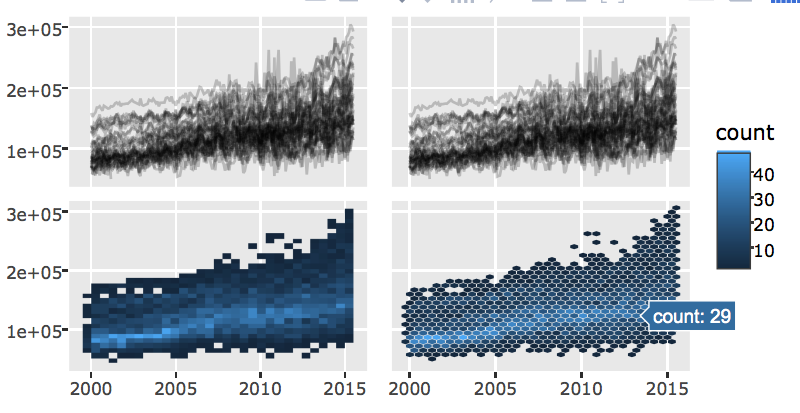
\includegraphics{screenshots/ggsubplot}
\caption{\label{fig:ggsubplot}Monthly median house price in the state of
Texas. The top row displays the raw data (by city) and the bottom row
shows 2D binning on the raw data. The binning is helpful for showing the
overall trend, but hovering on the lines in the top row helps reveal
more detailed information about each city.}
\end{figure}

\begin{rmdtip}
Although \textbf{ggplot2} does not have a \texttt{text} aesthetic, the
\texttt{ggplotly()} function recognizes this aesthetic and displays it
in the tooltip by default. In addition to providing a way to supply
``meta'' information, it also provides a way to customize your tooltips
(do this by restricting the tooltip to the text aesthetic --
\texttt{ggplotly(p,\ tooltip\ =\ "text")})
\end{rmdtip}

The \texttt{ggplotly()} function translates most things that you can do
in \textbf{ggplot2}, but not quite everything. To help demonstrate the
coverage, I've built a
\href{http://ropensci.github.io/plotly/ggplot2}{plotly version of the
ggplot2 docs}. This version of the docs displays the \texttt{ggplotly()}
version of each plot in a static form (to reduce page loading time), but
you can click any plot to view its interactive version. The next section
deomnstrates how to create plotly.js visualizations via the R package,
without \textbf{ggplot2}, via the \texttt{plot\_ly()} function. We'll
then leverage those concepts to
\protect\hyperlink{extending-ggplotly}{extend \texttt{ggplotly()}}.

\subsubsection{\texorpdfstring{The \texttt{plot\_ly()}
interface}{The plot\_ly() interface}}\label{the-plot_ly-interface}

\hypertarget{the-layered-grammar-of-graphics}{\paragraph{The Layered
Grammar of Graphics}\label{the-layered-grammar-of-graphics}}

The cognitive framework underlying the \texttt{plot\_ly()} interface
draws inspiration from the layered grammar of graphics (Wickham
\protect\hyperlink{ref-Wickham:2010hya}{2010}\protect\hyperlink{ref-Wickham:2010hya}{b}),
but in contrast to \texttt{ggplotly()}, it provides a more flexible and
direct interface to
\href{https://github.com/plotly/plotly.js}{plotly.js}. It is more direct
in the sense that it doesn't call \textbf{ggplot2}'s sometimes expensive
plot building routines, and it is more flexible in the sense that data
frames are not required, which is useful for visualizing matrices, as
shown in \protect\hyperlink{get-started}{Get Started}. Although data
frames are not required, using them is highly recommended, especially
when constructing a plot with multiple layers or groups.

When a data frame is associated with a \textbf{plotly} object, it allows
us to manipulate the data underlying that object in the same way we
would directly manipulate the data. Currently, \texttt{plot\_ly()}
borrows semantics from and provides special plotly methods for generic
functions in the \textbf{dplyr} and \textbf{tidyr} packages (Wickham and
Francois \protect\hyperlink{ref-dplyr}{2014}); (Wickham
\protect\hyperlink{ref-tidyr}{2016}\protect\hyperlink{ref-tidyr}{a}).
Most importantly, \texttt{plot\_ly()} recognizes and preserves groupings
created with \textbf{dplyr}'s \texttt{group\_by()} function.

\begin{Shaded}
\begin{Highlighting}[]
\KeywordTok{library}\NormalTok{(dplyr)}
\NormalTok{tx <-}\StringTok{ }\KeywordTok{group_by}\NormalTok{(txhousing, city)}
\CommentTok{# initiate a plotly object with date on x and median on y}
\NormalTok{p <-}\StringTok{ }\KeywordTok{plot_ly}\NormalTok{(tx, }\DataTypeTok{x =} \NormalTok{~date, }\DataTypeTok{y =} \NormalTok{~median)}
\CommentTok{# plotly_data() returns data associated with a plotly object, note the group attribute!}
\KeywordTok{plotly_data}\NormalTok{(p)}
\CommentTok{#> Source: local data frame [8,602 x 9]}
\CommentTok{#> Groups: city [46]}
\CommentTok{#> }
\CommentTok{#>      city  year month sales   volume median listings inventory  date}
\CommentTok{#>     <chr> <int> <int> <dbl>    <dbl>  <dbl>    <dbl>     <dbl> <dbl>}
\CommentTok{#> 1 Abilene  2000     1    72  5380000  71400      701       6.3  2000}
\CommentTok{#> 2 Abilene  2000     2    98  6505000  58700      746       6.6  2000}
\CommentTok{#> 3 Abilene  2000     3   130  9285000  58100      784       6.8  2000}
\CommentTok{#> 4 Abilene  2000     4    98  9730000  68600      785       6.9  2000}
\CommentTok{#> 5 Abilene  2000     5   141 10590000  67300      794       6.8  2000}
\CommentTok{#> 6 Abilene  2000     6   156 13910000  66900      780       6.6  2000}
\CommentTok{#> # ... with 8,596 more rows}
\end{Highlighting}
\end{Shaded}

Defining groups in this fashion ensures \texttt{plot\_ly()} will produce
at least one graphical mark per group.\footnote{In practice, it's easy
  to forget about ``lingering'' groups (e.g.,
  \texttt{mtcars\ \%\textgreater{}\%\ group\_by(vs,\ am)\ \%\textgreater{}\%\ summarise(s\ =\ sum(mpg))}),
  so in some cases, you may need to \texttt{ungroup()} your data before
  plotting it.} So far we've specified \texttt{x}/\texttt{y} attributes
in the plotly object \texttt{p}, but we have not yet specified the
geometric relation between these x/y pairs. Similar to
\texttt{geom\_line()} in \textbf{ggplot2}, the \texttt{add\_lines()}
function connects (a group of) x/y pairs with lines in the order of
their \texttt{x} values, which is useful when plotting time series as
shown in Figure \ref{fig:houston}.

\begin{Shaded}
\begin{Highlighting}[]
\CommentTok{# add a line highlighting houston}
\KeywordTok{add_lines}\NormalTok{(}
  \CommentTok{# plots one line per city since p knows city is a grouping variable}
  \KeywordTok{add_lines}\NormalTok{(p, }\DataTypeTok{alpha =} \FloatTok{0.2}\NormalTok{, }\DataTypeTok{name =} \StringTok{"Texan Cities"}\NormalTok{, }\DataTypeTok{hoverinfo =} \StringTok{"none"}\NormalTok{),}
  \DataTypeTok{name =} \StringTok{"Houston"}\NormalTok{, }\DataTypeTok{data =} \KeywordTok{filter}\NormalTok{(txhousing, city ==}\StringTok{ "Houston"}\NormalTok{)}
\NormalTok{)}
\end{Highlighting}
\end{Shaded}

\begin{figure}
\centering
\includegraphics{bookdown_files/figure-latex/houston-1.pdf}
\caption{\label{fig:houston}Monthly median house price in Houston in
comparison to other Texan cities.}
\end{figure}

The \textbf{plotly} package has a collection of \texttt{add\_*()}
functions, all of which inherit attributes defined in
\texttt{plot\_ly()}. These functions also inherit the data associated
with the plotly object provided as input, unless otherwise specified
with the \texttt{data} argument. I prefer to think about
\texttt{add\_*()} functions like a layer in \textbf{ggplot2}, which is
slightly different, but related to a plotly.js trace. In Figure
\ref{fig:houston}, there is a 1-to-1 correspondence between layers and
traces, but \texttt{add\_*()} functions do generate numerous traces
whenever mapping a discrete variable to a visual aesthetic (e.g.,
\href{scatterplots-discrete-color}{color}). In this case, since each
call to \texttt{add\_lines()} generates a single trace, it makes sense
to \texttt{name} the trace, so a sensible legend entry is created.

In the first layer of Figure \ref{fig:houston}, there is one line per
city, but all these lines belong a single trace. We \emph{could have}
produced one trace for each line, but this is way more computationally
expensive because, among other things, each trace produces a legend
entry and tries to display meaningful hover information. It is much more
efficient to render this layer as a single trace with missing values to
differentiate groups. In fact, this is exactly how the group aesthetic
is translated in \texttt{ggplotly()}; otherwise, layers with many groups
(e.g., \texttt{geom\_map()}) would be slow to render.

\hypertarget{the-data-plot-pipeline}{\paragraph{The
data-plot-pipeline}\label{the-data-plot-pipeline}}

Since every \textbf{plotly} function modifies a plotly object (or the
data underlying that object), we can express complex multi-layer plots
as a sequence (or, more specifically, a directed acyclic graph) of data
manipulations and mappings to the visual space. Moreover,
\textbf{plotly} functions are designed to take a plotly object as input,
and return a modified plotly object, making it easy to chain together
operations via the pipe operator (\texttt{\%\textgreater{}\%}) from the
\textbf{magrittr} package (Bache and Wickham
\protect\hyperlink{ref-magrittr}{2014}). Consequently, we can re-express
Figure \ref{fig:houston} in a much more readable and understandable
fashion.

\begin{Shaded}
\begin{Highlighting}[]
\NormalTok{allCities <-}\StringTok{ }\NormalTok{txhousing %>%}
\StringTok{  }\KeywordTok{group_by}\NormalTok{(city) %>%}
\StringTok{  }\KeywordTok{plot_ly}\NormalTok{(}\DataTypeTok{x =} \NormalTok{~date, }\DataTypeTok{y =} \NormalTok{~median) %>%}
\StringTok{  }\KeywordTok{add_lines}\NormalTok{(}\DataTypeTok{alpha =} \FloatTok{0.2}\NormalTok{, }\DataTypeTok{name =} \StringTok{"Texan Cities"}\NormalTok{, }\DataTypeTok{hoverinfo =} \StringTok{"none"}\NormalTok{)}

\NormalTok{allCities %>%}
\StringTok{  }\KeywordTok{filter}\NormalTok{(city ==}\StringTok{ "Houston"}\NormalTok{) %>%}
\StringTok{  }\KeywordTok{add_lines}\NormalTok{(}\DataTypeTok{name =} \StringTok{"Houston"}\NormalTok{)}
\end{Highlighting}
\end{Shaded}

\includegraphics{bookdown_files/figure-latex/unnamed-chunk-48-1.pdf}

Sometimes the directed acyclic graph property of a pipeline can be too
restrictive for certain types of plots. In this example, after filtering
the data down to Houston, there is no way to recover the original data
inside the pipeline. The \texttt{add\_fun()} function helps to
work-around this restriction\footnote{Credit to Winston Chang and Hadley
  Wickham for this idea. The \texttt{add\_fun()} is very much like
  \texttt{layer\_f()} function in \textbf{ggvis}.} -- it works by
applying a function to the plotly object, but does not affect the data
associated with the plotly object. This effectively provides a way to
isolate data transformations within the pipeline\footnote{Also,
  effectively putting a
  \href{http://www.memecreator.org/meme/yo-dawg-i-heard-u-like-pipelines-so-we-put-a-pipeline-in-your-pipeline}{pipeline
  inside a pipeline}}. Figure \ref{fig:houston-vs-sa} uses this idea to
highlight both Houston and San Antonio.

\begin{Shaded}
\begin{Highlighting}[]
\NormalTok{allCities %>%}
\StringTok{  }\KeywordTok{add_fun}\NormalTok{(function(plot) \{}
    \NormalTok{plot %>%}\StringTok{ }\KeywordTok{filter}\NormalTok{(city ==}\StringTok{ "Houston"}\NormalTok{) %>%}\StringTok{ }\KeywordTok{add_lines}\NormalTok{(}\DataTypeTok{name =} \StringTok{"Houston"}\NormalTok{)}
  \NormalTok{\}) %>%}
\StringTok{  }\KeywordTok{add_fun}\NormalTok{(function(plot) \{}
    \NormalTok{plot %>%}\StringTok{ }\KeywordTok{filter}\NormalTok{(city ==}\StringTok{ "San Antonio"}\NormalTok{) %>%}\StringTok{ }\KeywordTok{add_lines}\NormalTok{(}\DataTypeTok{name =} \StringTok{"San Antonio"}\NormalTok{)}
  \NormalTok{\})}
\end{Highlighting}
\end{Shaded}

\begin{figure}
\centering
\includegraphics{bookdown_files/figure-latex/houston-vs-sa-1.pdf}
\caption{\label{fig:houston-vs-sa}Monthly median house price in Houston and
San Antonio in comparison to other Texan cities.}
\end{figure}

It is useful to think of the function supplied to \texttt{add\_fun()} as
a ``layer'' function -- a function that accepts a plot object as input,
possibly applies a transformation to the data, and maps that data to
visual objects. To make layering functions more modular, flexible, and
expressive, the \texttt{add\_fun()} allows you to pass additional
arguments to a layer function. Figure \ref{fig:summary} makes use of
this pattern, by creating a reusable function for layering both a
particular city as well as the first, second, and third quartile of
median monthly house sales (by city).

\begin{Shaded}
\begin{Highlighting}[]
\CommentTok{# reusable function for highlighting a particular city}
\NormalTok{layer_city <-}\StringTok{ }\NormalTok{function(plot, name) \{}
  \NormalTok{plot %>%}\StringTok{ }\KeywordTok{filter}\NormalTok{(city ==}\StringTok{ }\NormalTok{name) %>%}\StringTok{ }\KeywordTok{add_lines}\NormalTok{(}\DataTypeTok{name =} \NormalTok{name)}
\NormalTok{\}}

\CommentTok{# reusable function for plotting overall median & IQR}
\NormalTok{layer_iqr <-}\StringTok{ }\NormalTok{function(plot) \{}
  \NormalTok{plot %>%}
\StringTok{    }\KeywordTok{group_by}\NormalTok{(date) %>%}\StringTok{ }
\StringTok{    }\KeywordTok{summarise}\NormalTok{(}
      \DataTypeTok{q1 =} \KeywordTok{quantile}\NormalTok{(median, }\FloatTok{0.25}\NormalTok{, }\DataTypeTok{na.rm =} \OtherTok{TRUE}\NormalTok{),}
      \DataTypeTok{m =} \KeywordTok{median}\NormalTok{(median, }\DataTypeTok{na.rm =} \OtherTok{TRUE}\NormalTok{),}
      \DataTypeTok{q3 =} \KeywordTok{quantile}\NormalTok{(median, }\FloatTok{0.75}\NormalTok{, }\DataTypeTok{na.rm =} \OtherTok{TRUE}\NormalTok{)}
    \NormalTok{) %>%}
\StringTok{    }\KeywordTok{add_lines}\NormalTok{(}\DataTypeTok{y =} \NormalTok{~m, }\DataTypeTok{name =} \StringTok{"median"}\NormalTok{, }\DataTypeTok{color =} \KeywordTok{I}\NormalTok{(}\StringTok{"black"}\NormalTok{)) %>%}
\StringTok{    }\KeywordTok{add_ribbons}\NormalTok{(}\DataTypeTok{ymin =} \NormalTok{~q1, }\DataTypeTok{ymax =} \NormalTok{~q3, }\DataTypeTok{name =} \StringTok{"IQR"}\NormalTok{, }\DataTypeTok{color =} \KeywordTok{I}\NormalTok{(}\StringTok{"black"}\NormalTok{))}
\NormalTok{\}}

\NormalTok{allCities %>%}
\StringTok{  }\KeywordTok{add_fun}\NormalTok{(layer_iqr) %>%}
\StringTok{  }\KeywordTok{add_fun}\NormalTok{(layer_city, }\StringTok{"Houston"}\NormalTok{) %>%}
\StringTok{  }\KeywordTok{add_fun}\NormalTok{(layer_city, }\StringTok{"San Antonio"}\NormalTok{)}
\CommentTok{#> Error in x[!is.na(x)]: object of type 'closure' is not subsettable}
\end{Highlighting}
\end{Shaded}

A layering function does not have to be a data-plot-pipeline itself. Its
only requirement on a layering function is that the first argument is a
plot object and it returns a plot object. This provides an opportunity
to say, fit a model to the plot data, extract the model components you
desire, and map those components to visuals. Furthermore, since
\textbf{plotly}'s \texttt{add\_*()} functions don't require a
data.frame, you can supply those components directly to attributes (as
long as they are well-defined), as done in Figure \ref{fig:forecast} via
the \textbf{forecast} package (Hyndman
\protect\hyperlink{ref-forecast}{2016}).

\begin{Shaded}
\begin{Highlighting}[]
\KeywordTok{library}\NormalTok{(forecast)}
\NormalTok{layer_forecast <-}\StringTok{ }\NormalTok{function(plot) \{}
  \NormalTok{d <-}\StringTok{ }\KeywordTok{plotly_data}\NormalTok{(plot)}
  \NormalTok{series <-}\StringTok{ }\KeywordTok{with}\NormalTok{(d, }
    \KeywordTok{ts}\NormalTok{(median, }\DataTypeTok{frequency =} \DecValTok{12}\NormalTok{, }\DataTypeTok{start =} \KeywordTok{c}\NormalTok{(}\DecValTok{2000}\NormalTok{, }\DecValTok{1}\NormalTok{), }\DataTypeTok{end =} \KeywordTok{c}\NormalTok{(}\DecValTok{2015}\NormalTok{, }\DecValTok{7}\NormalTok{))}
  \NormalTok{)}
  \NormalTok{fore <-}\StringTok{ }\KeywordTok{forecast}\NormalTok{(}\KeywordTok{ets}\NormalTok{(series), }\DataTypeTok{h =} \DecValTok{48}\NormalTok{, }\DataTypeTok{level =} \KeywordTok{c}\NormalTok{(}\DecValTok{80}\NormalTok{, }\DecValTok{95}\NormalTok{))}
  \NormalTok{plot %>%}
\StringTok{    }\KeywordTok{add_ribbons}\NormalTok{(}\DataTypeTok{x =} \KeywordTok{time}\NormalTok{(fore$mean), }\DataTypeTok{ymin =} \NormalTok{fore$lower[, }\DecValTok{2}\NormalTok{],}
                \DataTypeTok{ymax =} \NormalTok{fore$upper[, }\DecValTok{2}\NormalTok{], }\DataTypeTok{color =} \KeywordTok{I}\NormalTok{(}\StringTok{"gray95"}\NormalTok{), }
                \DataTypeTok{name =} \StringTok{"95% confidence"}\NormalTok{, }\DataTypeTok{inherit =} \OtherTok{FALSE}\NormalTok{) %>%}
\StringTok{    }\KeywordTok{add_ribbons}\NormalTok{(}\DataTypeTok{x =} \KeywordTok{time}\NormalTok{(fore$mean), }\DataTypeTok{ymin =} \NormalTok{fore$lower[, }\DecValTok{1}\NormalTok{],}
                \DataTypeTok{ymax =} \NormalTok{fore$upper[, }\DecValTok{1}\NormalTok{], }\DataTypeTok{color =} \KeywordTok{I}\NormalTok{(}\StringTok{"gray80"}\NormalTok{), }
                \DataTypeTok{name =} \StringTok{"80% confidence"}\NormalTok{, }\DataTypeTok{inherit =} \OtherTok{FALSE}\NormalTok{) %>%}
\StringTok{    }\KeywordTok{add_lines}\NormalTok{(}\DataTypeTok{x =} \KeywordTok{time}\NormalTok{(fore$mean), }\DataTypeTok{y =} \NormalTok{fore$mean, }\DataTypeTok{color =} \KeywordTok{I}\NormalTok{(}\StringTok{"blue"}\NormalTok{), }
              \DataTypeTok{name =} \StringTok{"prediction"}\NormalTok{)}
\NormalTok{\}}

\NormalTok{txhousing %>%}
\StringTok{  }\KeywordTok{group_by}\NormalTok{(city) %>%}
\StringTok{  }\KeywordTok{plot_ly}\NormalTok{(}\DataTypeTok{x =} \NormalTok{~date, }\DataTypeTok{y =} \NormalTok{~median) %>%}
\StringTok{  }\KeywordTok{add_lines}\NormalTok{(}\DataTypeTok{alpha =} \FloatTok{0.2}\NormalTok{, }\DataTypeTok{name =} \StringTok{"Texan Cities"}\NormalTok{, }\DataTypeTok{hoverinfo =} \StringTok{"none"}\NormalTok{) %>%}
\StringTok{  }\KeywordTok{add_fun}\NormalTok{(layer_iqr) %>%}
\StringTok{  }\KeywordTok{add_fun}\NormalTok{(layer_forecast)}
\CommentTok{#> Error in x[!is.na(x)]: object of type 'closure' is not subsettable}
\end{Highlighting}
\end{Shaded}

In summary, the ``data-plot-pipeline'' is desirable for a number of
reasons: (1) makes your code easier to read and understand, (2)
encourages you to think of both your data and plots using a single,
uniform data structure, which (3) makes it easy to combine and reuse
transformations. As it turns out, we can even use these ideas when
creating a plotly object via \texttt{ggplotly()}, as discused in the
next section \protect\hyperlink{extending-ggplotly}{Extending
\texttt{ggplotly()}}(extending-ggplotly.

\hypertarget{extending-ggplotly}{\subsection{\texorpdfstring{Extending
\texttt{ggplotly()}}{Extending ggplotly()}}\label{extending-ggplotly}}

\subsubsection{Customizing the layout}\label{customizing-the-layout}

Since the \texttt{ggplotly()} function returns a plotly object, we can
manipulate that object in the same way that we would manipulate any
other plotly object. A simple and useful application of this is to
specify interaction modes, like plotly.js'
\href{https://plot.ly/r/reference/\#layout-dragmode}{layout.dragmode}
for specifying the mode of click+drag events. Figure
\ref{fig:ggplotly-layout} demonstrates how the default for this
attribute can be modified via the \texttt{layout()} function.

\begin{Shaded}
\begin{Highlighting}[]
\NormalTok{p <-}\StringTok{ }\KeywordTok{ggplot}\NormalTok{(}\KeywordTok{fortify}\NormalTok{(gold), }\KeywordTok{aes}\NormalTok{(x, y)) +}\StringTok{ }\KeywordTok{geom_line}\NormalTok{()}
\NormalTok{gg <-}\StringTok{ }\KeywordTok{ggplotly}\NormalTok{(p)}
\KeywordTok{layout}\NormalTok{(gg, }\DataTypeTok{dragmode =} \StringTok{"pan"}\NormalTok{)}
\end{Highlighting}
\end{Shaded}

\begin{figure}
\centering
\includegraphics{bookdown_files/figure-latex/ggplotly-layout-1.pdf}
\caption{\label{fig:ggplotly-layout}Customizing the dragmode of an
interactive ggplot2 graph.}
\end{figure}

Perhaps a more useful application is to add a range slider to the
x-axis, which allows you to zoom on the x-axis, without losing the
global context. This is quite useful for quickly altering the limits of
your plot to achieve an optimal aspect ratio for your data (William S.
Cleveland \protect\hyperlink{ref-banking}{1988}), without losing the
global perspective. Figure \ref{fig:ggplotly-rangeslider} uses the
\texttt{rangeslider()} function to add a rangeslider to the plot.

\begin{Shaded}
\begin{Highlighting}[]
\KeywordTok{rangeslider}\NormalTok{(gg)}
\end{Highlighting}
\end{Shaded}

\begin{figure}
\centering
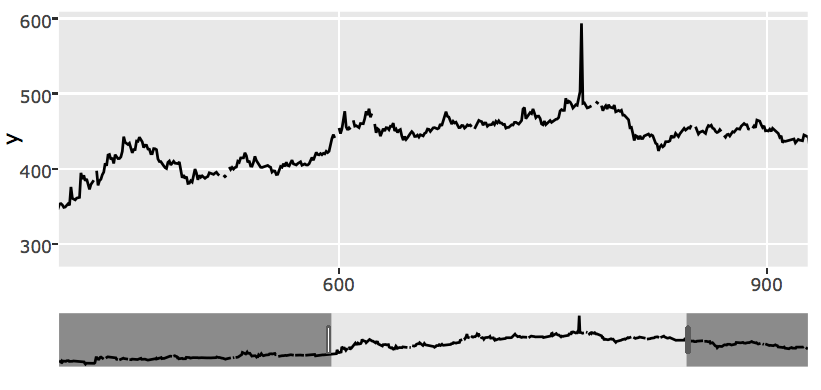
\includegraphics{screenshots/ggplotly-rangeslider}
\caption{\label{fig:ggplotly-rangeslider}Adding a rangeslider to an
interactive ggplot2 graph.}
\end{figure}

Since a single plotly object can only have one layout, modifying the
layout of \texttt{ggplotly()} is fairly easy, but it's trickier to
\protect\hyperlink{adding-layers}{add} and
\protect\hyperlink{modifying-layers}{modify} layers.

\hypertarget{adding-layers}{\subsubsection{Adding
layers}\label{adding-layers}}

Since \texttt{ggplotly()} returns a plotly object, and plotly objects
have data associated with them, we can effectively associate data from a
ggplot object with a plotly object, before or after summary statistics
have been applied. Since each ggplot layer owns a data frame, it is
useful to have some way to specify the particular layer of data of
interest, which is the point of the \texttt{layerData} argument in
\texttt{ggplotly()}. Also, when a particular layer applies a summary
statistic (e.g., \texttt{geom\_bin()}), or applies a model (e.g.,
\texttt{geom\_smooth()}) to the data, it might be useful to access the
output of that transformation, which is the point of the
\texttt{originalData} argument in \texttt{ggplotly()}.

\begin{Shaded}
\begin{Highlighting}[]
\NormalTok{p <-}\StringTok{ }\KeywordTok{ggplot}\NormalTok{(mtcars, }\KeywordTok{aes}\NormalTok{(}\DataTypeTok{x =} \NormalTok{wt, }\DataTypeTok{y =} \NormalTok{mpg)) +}
\StringTok{   }\KeywordTok{geom_point}\NormalTok{() +}\StringTok{ }\KeywordTok{geom_smooth}\NormalTok{()}
\NormalTok{p %>%}
\StringTok{  }\KeywordTok{ggplotly}\NormalTok{(}\DataTypeTok{layerData =} \DecValTok{2}\NormalTok{, }\DataTypeTok{originalData =} \OtherTok{FALSE}\NormalTok{) %>%}
\StringTok{  }\KeywordTok{plotly_data}\NormalTok{()}
\CommentTok{#> # A tibble: 80 × 13}
\CommentTok{#>       x     y  ymin  ymax    se PANEL group  colour   fill  size}
\CommentTok{#> * <dbl> <dbl> <dbl> <dbl> <dbl> <int> <int>   <chr>  <chr> <dbl>}
\CommentTok{#> 1  1.51  32.1  28.1  36.0  1.92     1    -1 #3366FF grey60     1}
\CommentTok{#> 2  1.56  31.7  28.2  35.2  1.72     1    -1 #3366FF grey60     1}
\CommentTok{#> 3  1.61  31.3  28.1  34.5  1.54     1    -1 #3366FF grey60     1}
\CommentTok{#> 4  1.66  30.9  28.0  33.7  1.39     1    -1 #3366FF grey60     1}
\CommentTok{#> 5  1.71  30.5  27.9  33.0  1.26     1    -1 #3366FF grey60     1}
\CommentTok{#> 6  1.76  30.0  27.7  32.4  1.16     1    -1 #3366FF grey60     1}
\CommentTok{#> # ... with 74 more rows, and 3 more variables: linetype <dbl>,}
\CommentTok{#> #   weight <dbl>, alpha <dbl>}
\end{Highlighting}
\end{Shaded}

This is the dataset ggplot2 uses to actually draw the fitted values (as
a line) and standard error bounds (as a ribbon). Figure
\ref{fig:se-annotations} uses this data to add additional information
about the model fit; in particular, it adds a vertical lines and
annotations at the x-values that are associated with the highest and
lowest amount uncertainty in y.

\begin{Shaded}
\begin{Highlighting}[]
\NormalTok{p %>%}
\StringTok{  }\KeywordTok{ggplotly}\NormalTok{(}\DataTypeTok{layerData =} \DecValTok{2}\NormalTok{, }\DataTypeTok{originalData =} \NormalTok{F) %>%}
\StringTok{  }\KeywordTok{add_fun}\NormalTok{(function(p) \{}
    \NormalTok{p %>%}\StringTok{ }\KeywordTok{slice}\NormalTok{(}\KeywordTok{which.max}\NormalTok{(se)) %>%}
\StringTok{      }\KeywordTok{add_segments}\NormalTok{(}\DataTypeTok{x =} \NormalTok{~x, }\DataTypeTok{xend =} \NormalTok{~x, }\DataTypeTok{y =} \NormalTok{~ymin, }\DataTypeTok{yend =} \NormalTok{~ymax) %>%}
\StringTok{      }\KeywordTok{add_annotations}\NormalTok{(}\StringTok{"Maximum uncertainty"}\NormalTok{, }\DataTypeTok{ax =} \DecValTok{60}\NormalTok{)}
  \NormalTok{\}) %>%}
\StringTok{  }\KeywordTok{add_fun}\NormalTok{(function(p) \{}
    \NormalTok{p %>%}\StringTok{ }\KeywordTok{slice}\NormalTok{(}\KeywordTok{which.min}\NormalTok{(se)) %>%}
\StringTok{      }\KeywordTok{add_segments}\NormalTok{(}\DataTypeTok{x =} \NormalTok{~x, }\DataTypeTok{xend =} \NormalTok{~x, }\DataTypeTok{y =} \NormalTok{~ymin, }\DataTypeTok{yend =} \NormalTok{~ymax) %>%}
\StringTok{      }\KeywordTok{add_annotations}\NormalTok{(}\StringTok{"Minimum uncertainty"}\NormalTok{)}
  \NormalTok{\})}
\end{Highlighting}
\end{Shaded}

\begin{figure}
\centering
\includegraphics{bookdown_files/figure-latex/se-annotations-1.pdf}
\caption{\label{fig:se-annotations}Leveraging data associated with a
\texttt{geom\_smooth()} layer to display additional information about
the model fit.}
\end{figure}

Although it is not used in this example, it worth noting that when
adding plotly layers to the output of \texttt{ggplotly()}, it will
inherit mappings from the ggplot aesthetic mapping, which may or may not
be desired, but the \texttt{inherit} argument in any of the
\texttt{add\_*()} functions may be set to \texttt{FALSE} to avoid this
behavoir.

\hypertarget{modifying-layers}{\subsubsection{Modifying
layers}\label{modifying-layers}}

As mentioned previously, \texttt{ggplotly()} translates each ggplot2
layer into one or more plotly.js traces. In this translation, it is
forced to make a number of assumptions about trace attribute values that
may or may not be appropriate for the use case. The \texttt{style()}
function is useful in this scenario, as it provides a way to modify
trace attribute values in a plotly object. Before using it, you may want
to inspect the actual traces in a given plotly object using the
\texttt{plotly\_json()} function. This function uses the
\textbf{listviewer} package to display a convenient interactive view of
the JSON object sent to plotly.js (de Jong and Russell
\protect\hyperlink{ref-listviewer}{2016}). By clicking on the arrow next
to the data element, you can see the traces (data) behind the plot. In
this case, we have three traces: one for the \texttt{geom\_point()}
layer and two for the \texttt{geom\_smooth()} layer.

\begin{Shaded}
\begin{Highlighting}[]
\KeywordTok{plotly_json}\NormalTok{(p)}
\end{Highlighting}
\end{Shaded}

\begin{figure}
\centering
\includegraphics{bookdown_files/figure-latex/listviewer-1.pdf}
\caption{\label{fig:listviewer}Using listviewer to inspect a plotly object.}
\end{figure}

Say, for example, we'd like to display information when hovering over
points, but not when hovering over the fitted values or error bounds.
The ggplot2 API has no semantics for making this distinction, but this
is easily done in plotly.js by setting the
\href{https://plot.ly/r/reference/\#scatter-hoverinfo}{hoverinfo}
attribute to \texttt{"none"}. Since the fitted values or error bounds
are contained in the second and third traces, we can hide the
information on just these traces using the \texttt{traces} attribute in
the \texttt{style()} function:

\begin{Shaded}
\begin{Highlighting}[]
\KeywordTok{style}\NormalTok{(p, }\DataTypeTok{hoverinfo =} \StringTok{"none"}\NormalTok{, }\DataTypeTok{traces =} \DecValTok{2}\NormalTok{:}\DecValTok{3}\NormalTok{)}
\end{Highlighting}
\end{Shaded}

\includegraphics{bookdown_files/figure-latex/unnamed-chunk-51-1.pdf}

\section{The plotly cookbook}\label{the-plotly-cookbook}

This chapter demonstrates the rendering capabilities of
\texttt{plot\_ly()} through a series of examples. The
\texttt{plot\_ly()} function provides a direct interface to plotly.js,
so anything in \href{https://plot.ly/r/reference/}{the figure reference}
can be specified via \texttt{plot\_ly()}, but this chapter will focus
more on the special semantics unique to the R package that can't be
found on the figure reference. Along the way, we will touch on some best
practices in visualization.

\hypertarget{scatter-traces}{\subsection{Scatter
traces}\label{scatter-traces}}

A plotly visualization is composed of one (or more) trace(s), and every
trace has a \texttt{type}. The default trace type, ``scatter'', can be
used to draw a large amount of geometries, and actually powers many of
the \texttt{add\_*()} functions such as \texttt{add\_markers()},
\texttt{add\_lines()}, \texttt{add\_paths()}, \texttt{add\_segments()},
\texttt{add\_ribbons()}, and \texttt{add\_polygons()}. Among other
things, these functions make assumptions about the
\href{https://plot.ly/r/reference/\#scatter-mode}{mode} of the scatter
trace, but any valid attribute(s) listed under the
\href{https://plot.ly/r/reference/\#scatter}{scatter section of the
figure reference} may be used to override defaults.

The \texttt{plot\_ly()} function has a number of arguments that make it
easier to scale data values to visual aesthetics (e.g.,
\texttt{color}/\texttt{colors}, \texttt{symbol}/\texttt{symbols},
\texttt{linetype}/\texttt{linetypes}, \texttt{size}/\texttt{sizes}).
These arguments are unique to the R package and dynamically determine
what objects in the figure reference to populate (e.g.,
\href{https://plot.ly/r/reference/\#scatter-marker-color}{\texttt{marker.color}}
vs \href{https://plot.ly/r/reference/\#scatter}{\texttt{line.color}}).
Generally speaking, the singular form of the argument defines the domain
of the scale (data) and the plural form defines the range of the scale
(visuals). To make it easier to alter default visual aesthetics (e.g.,
change all points from blue to black), ``AsIs'' values (values wrapped
with the \texttt{I()} function) are interpreted as values that already
live in visual space, and thus do not need to be scaled. The next
section on scatterplots explores detailed use of the
\texttt{color}/\texttt{colors}, \texttt{symbol}/\texttt{symbols}, \&
\texttt{size}/\texttt{sizes} arguments. The section on
\protect\hyperlink{line-plots}{lineplots} explores detailed use of the
\texttt{linetype}/\texttt{linetypes}.

\hypertarget{scatterplots}{\subsubsection{Scatterplots}\label{scatterplots}}

The scatterplot is useful for visualizing the correlation between two
quantitative variables. If you supply a numeric vector for x and y in
\texttt{plot\_ly()}, it defaults to a scatterplot, but you can also be
explicit about adding a layer of markers/points via the
\texttt{add\_markers()} function. A common problem with scatterplots is
overplotting, meaning that there are multiple observations occupying the
same (or similar) x/y locations. There are a few ways to combat
overplotting including: alpha transparency, hollow symbols, and
\protect\hyperlink{rectangular-binning-in-R}{2D density estimation}.
Figure \ref{fig:scatterplots} shows how alpha transparency and hollow
symbols can provide an improvement over the default.

\begin{Shaded}
\begin{Highlighting}[]
\KeywordTok{subplot}\NormalTok{(}
  \KeywordTok{plot_ly}\NormalTok{(mpg, }\DataTypeTok{x =} \NormalTok{~cty, }\DataTypeTok{y =} \NormalTok{~hwy, }\DataTypeTok{name =} \StringTok{"default"}\NormalTok{),}
  \KeywordTok{plot_ly}\NormalTok{(mpg, }\DataTypeTok{x =} \NormalTok{~cty, }\DataTypeTok{y =} \NormalTok{~hwy) %>%}\StringTok{ }\KeywordTok{add_markers}\NormalTok{(}\DataTypeTok{alpha =} \FloatTok{0.2}\NormalTok{, }\DataTypeTok{name =} \StringTok{"alpha"}\NormalTok{),}
  \KeywordTok{plot_ly}\NormalTok{(mpg, }\DataTypeTok{x =} \NormalTok{~cty, }\DataTypeTok{y =} \NormalTok{~hwy) %>%}\StringTok{ }\KeywordTok{add_markers}\NormalTok{(}\DataTypeTok{symbol =} \KeywordTok{I}\NormalTok{(}\DecValTok{1}\NormalTok{), }\DataTypeTok{name =} \StringTok{"hollow"}\NormalTok{)}
\NormalTok{)}
\end{Highlighting}
\end{Shaded}

\begin{figure}
\centering
\includegraphics{bookdown_files/figure-latex/scatterplots-1.pdf}
\caption{\label{fig:scatterplots}Three versions of a basic scatterplot}
\end{figure}

In Figure \ref{fig:scatterplots}, hollow circles are specified via
\texttt{symbol\ =\ I(1)}. By default, the \texttt{symbol} argument (as
well as the \texttt{color}/\texttt{size}/\texttt{linetype} arguments)
assumes value(s) are ``data'', which need to be mapped to a visual
palette (provided by \texttt{symbols}). Wrapping values with the
\texttt{I()} function notifies \texttt{plot\_ly()} that these values
should be taken ``AsIs''. If you compare the result of
\texttt{plot(1:25,\ 1:25,\ pch\ =\ 1:25)} to Figure \ref{fig:pch},
you'll see that \texttt{plot\_ly()} can translate R's plotting
characters (pch), but you can also use
\href{https://plot.ly/r/reference/\#scatter-marker-symbol}{plotly.js'
symbol syntax}, if you desire.

\begin{Shaded}
\begin{Highlighting}[]
\KeywordTok{subplot}\NormalTok{(}
  \KeywordTok{plot_ly}\NormalTok{(}\DataTypeTok{x =} \DecValTok{1}\NormalTok{:}\DecValTok{25}\NormalTok{, }\DataTypeTok{y =} \DecValTok{1}\NormalTok{:}\DecValTok{25}\NormalTok{, }\DataTypeTok{symbol =} \KeywordTok{I}\NormalTok{(}\DecValTok{1}\NormalTok{:}\DecValTok{25}\NormalTok{), }\DataTypeTok{name =} \StringTok{"pch"}\NormalTok{),}
  \KeywordTok{plot_ly}\NormalTok{(mpg, }\DataTypeTok{x =} \NormalTok{~cty, }\DataTypeTok{y =} \NormalTok{~hwy, }\DataTypeTok{symbol =} \NormalTok{~cyl, }\DataTypeTok{symbols =} \DecValTok{1}\NormalTok{:}\DecValTok{3}\NormalTok{, }\DataTypeTok{name =} \StringTok{"cyl"}\NormalTok{)}
\NormalTok{)}
\end{Highlighting}
\end{Shaded}

\begin{figure}
\centering
\includegraphics{bookdown_files/figure-latex/pch-1.pdf}
\caption{\label{fig:pch}Specifying symbol in a scatterplot}
\end{figure}

When mapping a numeric variable to \texttt{symbol}, it creates only one
trace, so no legend is generated. If you do want one trace per symbol,
make sure the variable you're mapping is a factor, as Figure
\ref{fig:symbol-factor} demonstrates. When plotting multiple traces, the
default plotly.js color scale will apply, but you can set the color of
every trace generated from this layer with
\texttt{color\ =\ I("black")}, or similar.

\begin{Shaded}
\begin{Highlighting}[]
\NormalTok{p <-}\StringTok{ }\KeywordTok{plot_ly}\NormalTok{(mpg, }\DataTypeTok{x =} \NormalTok{~cty, }\DataTypeTok{y =} \NormalTok{~hwy, }\DataTypeTok{alpha =} \FloatTok{0.3}\NormalTok{) }
\KeywordTok{subplot}\NormalTok{(}
  \KeywordTok{add_markers}\NormalTok{(p, }\DataTypeTok{symbol =} \NormalTok{~cyl, }\DataTypeTok{name =} \StringTok{"A single trace"}\NormalTok{),}
  \KeywordTok{add_markers}\NormalTok{(p, }\DataTypeTok{symbol =} \NormalTok{~}\KeywordTok{factor}\NormalTok{(cyl), }\DataTypeTok{color =} \KeywordTok{I}\NormalTok{(}\StringTok{"black"}\NormalTok{))}
\NormalTok{)}
\end{Highlighting}
\end{Shaded}

\begin{figure}
\centering
\includegraphics{bookdown_files/figure-latex/symbol-factor-1.pdf}
\caption{\label{fig:symbol-factor}Mapping symbol to a factor}
\end{figure}

The \texttt{color} argument adheres to similar rules as \texttt{symbol}:

\begin{itemize}
\item
  If numeric, \texttt{color} produces one trace, but
  \href{https://plot.ly/r/reference/\#scatter-marker-colorbar}{colorbar}
  is also generated to aide the decoding of colors back to data values.
  The \texttt{colorbar()} function can be used to customize the
  appearance of this automatically generated guide. The default
  colorscale is viridis, a perceptually-uniform colorscale (even when
  converted to black-and-white), and perceivable even to those with
  common forms of color blindness (Data Science
  \protect\hyperlink{ref-viridis}{2016}).
\item
  If discrete, \texttt{color} produces one trace per value, meaning a
  \href{https://plot.ly/r/reference/\#layout-legend}{legend} is
  generated. If an ordered factor, the default colorscale is viridis
  (Garnier \protect\hyperlink{ref-viridisLite}{2016}); otherwise, it is
  the ``Set2'' palette from the \textbf{RColorBrewer} package (Neuwirth
  \protect\hyperlink{ref-RColorBrewer}{2014})
\end{itemize}

\begin{Shaded}
\begin{Highlighting}[]
\NormalTok{p <-}\StringTok{ }\KeywordTok{plot_ly}\NormalTok{(mpg, }\DataTypeTok{x =} \NormalTok{~cty, }\DataTypeTok{y =} \NormalTok{~hwy, }\DataTypeTok{alpha =} \FloatTok{0.5}\NormalTok{)}
\KeywordTok{subplot}\NormalTok{(}
  \KeywordTok{add_markers}\NormalTok{(p, }\DataTypeTok{color =} \NormalTok{~cyl, }\DataTypeTok{showlegend =} \OtherTok{FALSE}\NormalTok{) %>%}\StringTok{ }
\StringTok{    }\KeywordTok{colorbar}\NormalTok{(}\DataTypeTok{title =} \StringTok{"Viridis"}\NormalTok{, }\DataTypeTok{len =} \DecValTok{1}\NormalTok{/}\DecValTok{2}\NormalTok{, }\DataTypeTok{y =} \DecValTok{1}\NormalTok{),}
  \KeywordTok{add_markers}\NormalTok{(p, }\DataTypeTok{color =} \NormalTok{~}\KeywordTok{factor}\NormalTok{(cyl))}
\NormalTok{) %>%}\StringTok{ }\KeywordTok{layout}\NormalTok{(}\DataTypeTok{showlegend =} \OtherTok{TRUE}\NormalTok{)}
\end{Highlighting}
\end{Shaded}

\begin{figure}
\centering
\includegraphics{screenshots/color-types}
\caption{\label{fig:color-types}Variations on a numeric color mapping.}
\end{figure}

There are a number of ways to alter the default colorscale via the
\texttt{colors} argument. This argument excepts: (1) a color brewer
palette name (see the row names of
\texttt{RColorBrewer::brewer.pal.info} for valid names), (2) a vector of
colors to interpolate, or (3) a color interpolation function like
\texttt{colorRamp()} or \texttt{scales::colour\_ramp()}. Although this
grants a lot of flexibility, one should be concious of using a
sequential colorscale for numeric variables (\& ordered factors) as
shown in \ref{fig:color-numeric}, and a qualitative colorscale for
discrete variables as shown in \ref{fig:color-discrete}. (TODO: touch on
lurking variables?)

\begin{Shaded}
\begin{Highlighting}[]
\KeywordTok{subplot}\NormalTok{(}
  \KeywordTok{add_markers}\NormalTok{(p, }\DataTypeTok{color =} \NormalTok{~cyl, }\DataTypeTok{colors =} \KeywordTok{c}\NormalTok{(}\StringTok{"#132B43"}\NormalTok{, }\StringTok{"#56B1F7"}\NormalTok{)) %>%}
\StringTok{    }\KeywordTok{colorbar}\NormalTok{(}\DataTypeTok{title =} \StringTok{"ggplot2 default"}\NormalTok{, }\DataTypeTok{len =} \DecValTok{1}\NormalTok{/}\DecValTok{3}\NormalTok{, }\DataTypeTok{y =} \DecValTok{1}\NormalTok{),}
  \KeywordTok{add_markers}\NormalTok{(p, }\DataTypeTok{color =} \NormalTok{~cyl, }\DataTypeTok{colors =} \NormalTok{viridisLite::}\KeywordTok{inferno}\NormalTok{(}\DecValTok{10}\NormalTok{)) %>%}\StringTok{ }
\StringTok{    }\KeywordTok{colorbar}\NormalTok{(}\DataTypeTok{title =} \StringTok{"Inferno"}\NormalTok{, }\DataTypeTok{len =} \DecValTok{1}\NormalTok{/}\DecValTok{3}\NormalTok{, }\DataTypeTok{y =} \DecValTok{2}\NormalTok{/}\DecValTok{3}\NormalTok{),}
  \KeywordTok{add_markers}\NormalTok{(p, }\DataTypeTok{color =} \NormalTok{~cyl, }\DataTypeTok{colors =} \KeywordTok{colorRamp}\NormalTok{(}\KeywordTok{c}\NormalTok{(}\StringTok{"red"}\NormalTok{, }\StringTok{"white"}\NormalTok{, }\StringTok{"blue"}\NormalTok{))) %>%}\StringTok{ }
\StringTok{    }\KeywordTok{colorbar}\NormalTok{(}\DataTypeTok{title =} \StringTok{"colorRamp"}\NormalTok{, }\DataTypeTok{len =} \DecValTok{1}\NormalTok{/}\DecValTok{3}\NormalTok{, }\DataTypeTok{y =} \DecValTok{1}\NormalTok{/}\DecValTok{3}\NormalTok{)}
\NormalTok{)}
\end{Highlighting}
\end{Shaded}

\begin{figure}
\centering
\includegraphics{screenshots/color-numeric}
\caption{\label{fig:color-numeric}Three variations on a numeric color
mapping}
\end{figure}

\begin{Shaded}
\begin{Highlighting}[]
\KeywordTok{subplot}\NormalTok{(}
  \KeywordTok{add_markers}\NormalTok{(p, }\DataTypeTok{color =} \NormalTok{~}\KeywordTok{factor}\NormalTok{(cyl), }\DataTypeTok{colors =} \StringTok{"Pastel1"}\NormalTok{),}
  \KeywordTok{add_markers}\NormalTok{(p, }\DataTypeTok{color =} \NormalTok{~}\KeywordTok{factor}\NormalTok{(cyl), }\DataTypeTok{colors =} \KeywordTok{colorRamp}\NormalTok{(}\KeywordTok{c}\NormalTok{(}\StringTok{"red"}\NormalTok{, }\StringTok{"blue"}\NormalTok{))),}
  \KeywordTok{add_markers}\NormalTok{(p, }\DataTypeTok{color =} \NormalTok{~}\KeywordTok{factor}\NormalTok{(cyl), }
              \DataTypeTok{colors =} \KeywordTok{c}\NormalTok{(}\StringTok{`}\DataTypeTok{4}\StringTok{`} \NormalTok{=}\StringTok{ "red"}\NormalTok{, }\StringTok{`}\DataTypeTok{5}\StringTok{`} \NormalTok{=}\StringTok{ "black"}\NormalTok{, }\StringTok{`}\DataTypeTok{6}\StringTok{`} \NormalTok{=}\StringTok{ "blue"}\NormalTok{, }\StringTok{`}\DataTypeTok{8}\StringTok{`} \NormalTok{=}\StringTok{ "green"}\NormalTok{))}
\NormalTok{) %>%}\StringTok{ }\KeywordTok{layout}\NormalTok{(}\DataTypeTok{showlegend =} \OtherTok{FALSE}\NormalTok{)}
\end{Highlighting}
\end{Shaded}

\begin{figure}
\centering
\includegraphics{bookdown_files/figure-latex/color-discrete-1.pdf}
\caption{\label{fig:color-discrete}Three variations on a discrete color
mapping}
\end{figure}

For scatterplots, the \texttt{size} argument controls the area of
markers (unless otherwise specified via
\href{https://plot.ly/r/reference/\#scatter-marker-sizemode}{sizemode}),
and \emph{must} be a numeric variable. The \texttt{sizes} argument
controls the minimum and maximum size of circles, in pixels:

\begin{Shaded}
\begin{Highlighting}[]
\KeywordTok{subplot}\NormalTok{(}
  \KeywordTok{add_markers}\NormalTok{(p, }\DataTypeTok{size =} \NormalTok{~cyl, }\DataTypeTok{name =} \StringTok{"default"}\NormalTok{),}
  \KeywordTok{add_markers}\NormalTok{(p, }\DataTypeTok{size =} \NormalTok{~cyl, }\DataTypeTok{sizes =} \KeywordTok{c}\NormalTok{(}\DecValTok{1}\NormalTok{, }\DecValTok{500}\NormalTok{), }\DataTypeTok{name =} \StringTok{"custom"}\NormalTok{)}
\NormalTok{)}
\end{Highlighting}
\end{Shaded}

\includegraphics{bookdown_files/figure-latex/unnamed-chunk-53-1.pdf}

\paragraph{3D scatterplots}\label{d-scatterplots}

To make a 3D scatterplot, just add a \texttt{z} attribute:

\begin{Shaded}
\begin{Highlighting}[]
\KeywordTok{plot_ly}\NormalTok{(mpg, }\DataTypeTok{x =} \NormalTok{~cty, }\DataTypeTok{y =} \NormalTok{~hwy, }\DataTypeTok{z =} \NormalTok{~cyl) %>%}
\StringTok{  }\KeywordTok{add_markers}\NormalTok{(}\DataTypeTok{color =} \NormalTok{~cyl)}
\end{Highlighting}
\end{Shaded}

\begin{figure}
\centering
\includegraphics{screenshots/3D-scatterplot}
\caption{\label{fig:3D-scatterplot}A 3D scatterplot}
\end{figure}

\hypertarget{scatterplot-matrices}{\paragraph{Scatterplot
matrices}\label{scatterplot-matrices}}

Scatterplot matrices \emph{can} be made via \texttt{plot\_ly()} and
\texttt{subplot()}, but \texttt{ggplotly()} has a special method for
translating ggmatrix objects from the \textbf{GGally} package to plotly
objects (Schloerke et al. \protect\hyperlink{ref-GGally}{2016}). These
objects are essentially a matrix of ggplot objects and are the
underlying data structure which powers higher level functions in
\textbf{GGally}, such as \texttt{ggpairs()} -- a function for creating a
generalized pairs plot (Emerson et al.
\protect\hyperlink{ref-gpp}{2013}). The generalized pairs plot can be
motivated as a generalization of the scatterplot matrix with support for
categorical variables and different visual representations of the data
powered by the grammar of graphics. Figure \ref{fig:ggpairs} shows an
interactive version of the generalized pairs plot made via
\texttt{ggpairs()} and \texttt{ggplotly()}. In
\protect\hyperlink{linking-views-without-shiny}{Linking views without
shiny}, we explore how this framework can be extended to enable linked
brushing in the generalized pairs plot.

\begin{Shaded}
\begin{Highlighting}[]
\NormalTok{pm <-}\StringTok{ }\NormalTok{GGally::}\KeywordTok{ggpairs}\NormalTok{(iris)}
\KeywordTok{ggplotly}\NormalTok{(pm)}
\end{Highlighting}
\end{Shaded}

\begin{figure}
\centering
\includegraphics{screenshots/ggpairs}
\caption{\label{fig:ggpairs}An interactive version of the generalized pairs
plot made via the \texttt{ggpairs()} function from the \textbf{GGally}
package}
\end{figure}

\subsubsection{Dotplots \& error bars}\label{dotplots-error-bars}

A dotplot is similar to a scatterplot, except instead of two numeric
axes, one is categorical. The usual goal of a dotplot is to compare
value(s) on a numerical scale over numerous categories. In this context,
dotplots are preferrable to pie charts since comparing position along a
common scale is much easier than comparing angle or area (Cleveland and
McGill \protect\hyperlink{ref-graphical-perception}{1984}); (Bostock
\protect\hyperlink{ref-crowdsourcing-graphical-perception}{2010}).
Furthermore, dotplots can be preferrable to bar charts, especially when
comparing values within a narrow range far away from 0 (Few
\protect\hyperlink{ref-few-values}{2006}). Also, when presenting point
estimates, and uncertainty associated with those estimates, bar charts
tend to exaggerate the difference in point estimates, and lose focus on
uncertainty (Messing \protect\hyperlink{ref-messing}{2012}).

A popular application for dotplots (with error bars) is the so-called
``coefficient plot'' for visualizing the point estimates of coefficients
and their standard error. The \texttt{coefplot()} function in the
\textbf{coefplot} package (Lander
\protect\hyperlink{ref-coefplot}{2016}) and the \texttt{ggcoef()}
function in the \textbf{GGally} both produce coefficient plots for many
types of model objects in R using \textbf{ggplot2}, which we can
translate to plotly via \texttt{ggplotly()}. Since these packages use
points and segments to draw the coefficient plots, the hover information
is not the best, and it'd be better to use
\href{https://plot.ly/r/reference/\#scatter-error_x}{error objects}.
Figure \ref{fig:coefplot} uses the \texttt{tidy()} function from the
\textbf{broom} package (Robinson
\protect\hyperlink{ref-broom}{2016}\protect\hyperlink{ref-broom}{a}) to
obtain a data frame with one row per model coefficient, and produce a
coefficient plot with error bars along the x-axis.

\begin{Shaded}
\begin{Highlighting}[]
\NormalTok{m <-}\StringTok{ }\KeywordTok{lm}\NormalTok{(Sepal.Length ~}\StringTok{ }\NormalTok{Sepal.Width *}\StringTok{ }\NormalTok{Petal.Length *}\StringTok{ }\NormalTok{Petal.Width, }\DataTypeTok{data =} \NormalTok{iris)}
\CommentTok{# arrange by estimate, then make term a factor to order categories in the plot}
\NormalTok{d <-}\StringTok{ }\NormalTok{broom::}\KeywordTok{tidy}\NormalTok{(m) %>%}\StringTok{ }
\StringTok{  }\KeywordTok{arrange}\NormalTok{(}\KeywordTok{desc}\NormalTok{(estimate)) %>%}
\StringTok{  }\KeywordTok{mutate}\NormalTok{(}\DataTypeTok{term =} \KeywordTok{factor}\NormalTok{(term, }\DataTypeTok{levels =} \NormalTok{term))}
\KeywordTok{plot_ly}\NormalTok{(d, }\DataTypeTok{x =} \NormalTok{~estimate, }\DataTypeTok{y =} \NormalTok{~term) %>%}
\StringTok{  }\KeywordTok{add_markers}\NormalTok{(}\DataTypeTok{error_x =} \NormalTok{~}\KeywordTok{list}\NormalTok{(}\DataTypeTok{value =} \NormalTok{std.error)) %>%}
\StringTok{  }\KeywordTok{layout}\NormalTok{(}\DataTypeTok{margin =} \KeywordTok{list}\NormalTok{(}\DataTypeTok{l =} \DecValTok{200}\NormalTok{))}
\end{Highlighting}
\end{Shaded}

\begin{figure}
\centering
\includegraphics{bookdown_files/figure-latex/coefplot-1.pdf}
\caption{\label{fig:coefplot}A coefficient plot}
\end{figure}

\hypertarget{line-plots}{\subsubsection{Line plots}\label{line-plots}}

This section surveys useful applications of \texttt{add\_lines()} and
\texttt{add\_paths()}. The only difference between these functions is
that \texttt{add\_lines()} connects x/y pairs from left to right,
instead of the order in which the data appears. Both functions
understand the \texttt{color}, \texttt{linetype}, and \texttt{alpha}
attributes\footnote{plotly.js currently
  \href{https://github.com/plotly/plotly.js/issues/147}{does not support
  data arrays for \texttt{scatter.line.width} or
  \texttt{scatter.line.color}}, meaning a single line trace can only
  have one width/color in 2D line plot, and consequently numeric
  \texttt{color}/\texttt{size} mappings won't work}, as well as
groupings defined by \texttt{group\_by()}.

Figure \ref{fig:houston} uses \texttt{group\_by()} to plot one line per
city in the \texttt{txhousing} dataset using a \emph{single} trace.
Since there can only be one tooltip per trace, hovering over that plot
does not reveal useful information. Although plotting many traces can be
computationally expensive, it is necessary in order to display better
information on hover. Since the \texttt{color} argument produces one
trace per value (if the variable (\texttt{city}) is discrete), hovering
on Figure \ref{fig:many-traces} reveals the top \textasciitilde{}10
cities at a given x value. Since 46 colors is too many to perceive in a
single plot, Figure \ref{fig:many-traces} also restricts the set of
possible \texttt{colors} to black.

\begin{Shaded}
\begin{Highlighting}[]
\KeywordTok{plot_ly}\NormalTok{(txhousing, }\DataTypeTok{x =} \NormalTok{~date, }\DataTypeTok{y =} \NormalTok{~median) %>%}
\StringTok{  }\KeywordTok{add_lines}\NormalTok{(}\DataTypeTok{color =} \NormalTok{~city, }\DataTypeTok{colors =} \StringTok{"black"}\NormalTok{, }\DataTypeTok{alpha =} \FloatTok{0.2}\NormalTok{)}
\end{Highlighting}
\end{Shaded}

\begin{figure}
\centering
\includegraphics{screenshots/many-traces}
\caption{\label{fig:many-traces}Median house sales with one trace per city.}
\end{figure}

Generally speaking, it's hard to perceive more than 8 different
colors/linetypes/symbols in a given plot, so sometimes we have to filter
data to use these effectively. Here we use the \textbf{dplyr} package to
find the top 5 cities in terms of average monthly sales (\texttt{top5}),
then effectively filter the original data to contain just these cities
via \texttt{semi\_join()}. Once we have the data is filtered, mapping
city to \texttt{color} or \texttt{linetype} is trivial. The color
palette can be altered via the \texttt{colors} argument, and follows the
same rules as \protect\hyperlink{scatterplots}{scatterplots}. The
linetype palette can be altered via the \texttt{linetypes} argument, and
accepts R's
\href{https://github.com/wch/r-source/blob/e5b21d0397c607883ff25cca379687b86933d730/src/library/graphics/man/par.Rd\#L726-L743}{\texttt{lty}
values} or plotly.js
\href{https://plot.ly/r/reference/\#scatter-line-dash}{dash values}.

\begin{Shaded}
\begin{Highlighting}[]
\KeywordTok{library}\NormalTok{(dplyr)}
\NormalTok{top5 <-}\StringTok{ }\NormalTok{txhousing %>%}
\StringTok{  }\KeywordTok{group_by}\NormalTok{(city) %>%}
\StringTok{  }\KeywordTok{summarise}\NormalTok{(}\DataTypeTok{m =} \KeywordTok{mean}\NormalTok{(sales, }\DataTypeTok{na.rm =} \OtherTok{TRUE}\NormalTok{)) %>%}
\StringTok{  }\KeywordTok{arrange}\NormalTok{(}\KeywordTok{desc}\NormalTok{(m)) %>%}
\StringTok{  }\KeywordTok{top_n}\NormalTok{(}\DecValTok{5}\NormalTok{)}

\NormalTok{p <-}\StringTok{ }\KeywordTok{semi_join}\NormalTok{(txhousing, top5, }\DataTypeTok{by =} \StringTok{"city"}\NormalTok{) %>%}
\StringTok{  }\KeywordTok{plot_ly}\NormalTok{(}\DataTypeTok{x =} \NormalTok{~date, }\DataTypeTok{y =} \NormalTok{~median)}

\KeywordTok{subplot}\NormalTok{(}
  \KeywordTok{add_lines}\NormalTok{(p, }\DataTypeTok{color =} \NormalTok{~city),}
  \KeywordTok{add_lines}\NormalTok{(p, }\DataTypeTok{linetype =} \NormalTok{~city),}
  \DataTypeTok{shareX =} \OtherTok{TRUE}\NormalTok{, }\DataTypeTok{nrows =} \DecValTok{2}
\NormalTok{)}
\end{Highlighting}
\end{Shaded}

\includegraphics{bookdown_files/figure-latex/unnamed-chunk-54-1.pdf}

\paragraph{Density plots}\label{density-plots-1}

In \protect\hyperlink{bars-histograms}{Bars \& histograms}, we leveraged
a number of algorithms in R for computing the ``optimal'' number of bins
for a histogram, via \texttt{hist()}, and routing those results to
\texttt{add\_bars()}. We can leverage the \texttt{density()} function
for computing kernel density estimates in a similar way, and routing the
results to \texttt{add\_lines()}, as is done in \ref{fig:densities}.

\begin{Shaded}
\begin{Highlighting}[]
\NormalTok{kerns <-}\StringTok{ }\KeywordTok{c}\NormalTok{(}\StringTok{"gaussian"}\NormalTok{, }\StringTok{"epanechnikov"}\NormalTok{, }\StringTok{"rectangular"}\NormalTok{, }
          \StringTok{"triangular"}\NormalTok{, }\StringTok{"biweight"}\NormalTok{, }\StringTok{"cosine"}\NormalTok{, }\StringTok{"optcosine"}\NormalTok{)}
\NormalTok{p <-}\StringTok{ }\KeywordTok{plot_ly}\NormalTok{()}
\NormalTok{for (k in kerns) \{}
  \NormalTok{d <-}\StringTok{ }\KeywordTok{density}\NormalTok{(txhousing$median, }\DataTypeTok{kernel =} \NormalTok{k, }\DataTypeTok{na.rm =} \OtherTok{TRUE}\NormalTok{)}
  \NormalTok{p <-}\StringTok{ }\KeywordTok{add_lines}\NormalTok{(p, }\DataTypeTok{x =} \NormalTok{d$x, }\DataTypeTok{y =} \NormalTok{d$y, }\DataTypeTok{name =} \NormalTok{k)}
\NormalTok{\}}
\KeywordTok{layout}\NormalTok{(p, }\DataTypeTok{xaxis =} \KeywordTok{list}\NormalTok{(}\DataTypeTok{title =} \StringTok{"Median monthly price"}\NormalTok{))}
\end{Highlighting}
\end{Shaded}

\begin{figure}
\centering
\includegraphics{bookdown_files/figure-latex/densities-1.pdf}
\caption{\label{fig:densities}Various kernel density estimates.}
\end{figure}

\paragraph{Parallel Coordinates}\label{parallel-coordinates}

One very useful, but often overlooked, visualization technique is the
parallel coordinates plot. Parallel coordinates provide a way to compare
values along a common (or non-aligned) positional scale(s) -- the most
basic of all perceptual tasks -- in more than 3 dimensions (Cleveland
and McGill \protect\hyperlink{ref-graphical-perception}{1984}). Usually
each line represents every measurement for a given row (or observation)
in a data set. When measurements are on very different scales, some care
must be taken, and variables must transformed to be put on a common
scale. As Figure \ref{fig:pcp-common} shows, even when variables are
measured on a similar scale, it can still be a informative to transform
variables in different ways.

\begin{Shaded}
\begin{Highlighting}[]
\NormalTok{iris$obs <-}\StringTok{ }\KeywordTok{seq_len}\NormalTok{(}\KeywordTok{nrow}\NormalTok{(iris))}
\NormalTok{iris_pcp <-}\StringTok{ }\NormalTok{function(}\DataTypeTok{transform =} \NormalTok{identity) \{}
  \NormalTok{iris[] <-}\StringTok{ }\NormalTok{purrr::}\KeywordTok{map_if}\NormalTok{(iris, is.numeric, transform)}
  \NormalTok{tidyr::}\KeywordTok{gather}\NormalTok{(iris, variable, value, -Species, -obs) %>%}\StringTok{ }
\StringTok{    }\KeywordTok{group_by}\NormalTok{(obs) %>%}\StringTok{ }
\StringTok{    }\KeywordTok{plot_ly}\NormalTok{(}\DataTypeTok{x =} \NormalTok{~variable, }\DataTypeTok{y =} \NormalTok{~value, }\DataTypeTok{color =} \NormalTok{~Species) %>%}\StringTok{ }
\StringTok{    }\KeywordTok{add_lines}\NormalTok{(}\DataTypeTok{alpha =} \FloatTok{0.3}\NormalTok{)}
\NormalTok{\}}
\KeywordTok{subplot}\NormalTok{(}
  \KeywordTok{iris_pcp}\NormalTok{(), }
  \KeywordTok{iris_pcp}\NormalTok{(scale),}
  \KeywordTok{iris_pcp}\NormalTok{(scales::rescale)}
\NormalTok{) %>%}\StringTok{ }\KeywordTok{hide_legend}\NormalTok{()}
\end{Highlighting}
\end{Shaded}

\begin{figure}
\centering
\includegraphics{bookdown_files/figure-latex/pcp-common-1.pdf}
\caption{\label{fig:pcp-common}Parallel coordinates plots of the Iris
dataset. On the left is the raw measurements. In the middle, each
variable is scaled to have mean of 0 and standard deviation of 1. On the
right, each variable is scaled to have a minimum of 0 and a maximum of
1.}
\end{figure}

It is also worth noting that the \textbf{GGally} offers a
\texttt{ggparcoord()} function which creates parallel coordinate plots
via \textbf{ggplot2}, which we can convert to plotly via
\texttt{ggplotly()}. In \protect\hyperlink{linked-highlighting}{linked
highlighting}, parallel coordinates are linked to lower dimensional (but
sometimes higher resolution) graphics of related data to guide
multi-variate data exploration.

\paragraph{3D paths}\label{d-paths}

To make a path in 3D, use \texttt{add\_paths()} in the same way you
would for a 2D path, but add a third variable \texttt{z}, as Figure
\ref{fig:3D-paths} does.

\begin{Shaded}
\begin{Highlighting}[]
\KeywordTok{plot_ly}\NormalTok{(mpg, }\DataTypeTok{x =} \NormalTok{~cty, }\DataTypeTok{y =} \NormalTok{~hwy, }\DataTypeTok{z =} \NormalTok{~cyl) %>%}
\StringTok{  }\KeywordTok{add_paths}\NormalTok{(}\DataTypeTok{color =} \NormalTok{~displ)}
\end{Highlighting}
\end{Shaded}

\begin{figure}
\centering
\includegraphics{screenshots/3D-paths}
\caption{\label{fig:3D-paths}A path in 3D}
\end{figure}

Figure \ref{fig:3D-lines} uses \texttt{add\_lines()} instead of
\texttt{add\_paths()} to ensure the points are connected by the x axis
instead of the row ordering.

\begin{Shaded}
\begin{Highlighting}[]
\KeywordTok{plot_ly}\NormalTok{(mpg, }\DataTypeTok{x =} \NormalTok{~cty, }\DataTypeTok{y =} \NormalTok{~hwy, }\DataTypeTok{z =} \NormalTok{~cyl) %>%}
\StringTok{  }\KeywordTok{add_lines}\NormalTok{(}\DataTypeTok{color =} \NormalTok{~displ)}
\end{Highlighting}
\end{Shaded}

\begin{figure}
\centering
\includegraphics{screenshots/3D-lines}
\caption{\label{fig:3D-lines}A 3D line plot}
\end{figure}

\subsubsection{Segments}\label{segments}

The \texttt{add\_segments()} function essentially provides a way to
connect two points ((\texttt{x}, \texttt{y}) to (\texttt{xend},
\texttt{yend})) with a line. Segments form the building blocks for many
useful chart types, including candlestick charts, a popular way to
visualize stock prices. Figure \ref{fig:candlestick} uses the
\textbf{quantmod} package (Ryan \protect\hyperlink{ref-quantmod}{2016})
to obtain stock price data for Microsoft and plots two segments for each
day: one to encode the opening/closing values, and one to encode the
daily high/low.

\begin{Shaded}
\begin{Highlighting}[]
\KeywordTok{library}\NormalTok{(quantmod)}
\NormalTok{msft <-}\StringTok{ }\KeywordTok{getSymbols}\NormalTok{(}\StringTok{"MSFT"}\NormalTok{, }\DataTypeTok{auto.assign =} \NormalTok{F)}
\NormalTok{dat <-}\StringTok{ }\KeywordTok{as.data.frame}\NormalTok{(msft)}
\NormalTok{dat$date <-}\StringTok{ }\KeywordTok{index}\NormalTok{(msft)}
\NormalTok{dat <-}\StringTok{ }\KeywordTok{subset}\NormalTok{(dat, date >=}\StringTok{ "2016-01-01"}\NormalTok{)}

\KeywordTok{names}\NormalTok{(dat) <-}\StringTok{ }\KeywordTok{sub}\NormalTok{(}\StringTok{"^MSFT}\CharTok{\textbackslash{}\textbackslash{}}\StringTok{."}\NormalTok{, }\StringTok{""}\NormalTok{, }\KeywordTok{names}\NormalTok{(dat))}

\KeywordTok{plot_ly}\NormalTok{(dat, }\DataTypeTok{x =} \NormalTok{~date, }\DataTypeTok{xend =} \NormalTok{~date, }\DataTypeTok{color =} \NormalTok{~Close >}\StringTok{ }\NormalTok{Open, }
        \DataTypeTok{colors =} \KeywordTok{c}\NormalTok{(}\StringTok{"red"}\NormalTok{, }\StringTok{"forestgreen"}\NormalTok{), }\DataTypeTok{hoverinfo =} \StringTok{"none"}\NormalTok{) %>%}
\StringTok{  }\KeywordTok{add_segments}\NormalTok{(}\DataTypeTok{y =} \NormalTok{~Low, }\DataTypeTok{yend =} \NormalTok{~High, }\DataTypeTok{size =} \KeywordTok{I}\NormalTok{(}\DecValTok{1}\NormalTok{)) %>%}
\StringTok{  }\KeywordTok{add_segments}\NormalTok{(}\DataTypeTok{y =} \NormalTok{~Open, }\DataTypeTok{yend =} \NormalTok{~Close, }\DataTypeTok{size =} \KeywordTok{I}\NormalTok{(}\DecValTok{3}\NormalTok{)) %>%}
\StringTok{  }\KeywordTok{layout}\NormalTok{(}\DataTypeTok{showlegend =} \OtherTok{FALSE}\NormalTok{, }\DataTypeTok{yaxis =} \KeywordTok{list}\NormalTok{(}\DataTypeTok{title =} \StringTok{"Price"}\NormalTok{)) %>%}
\StringTok{  }\KeywordTok{rangeslider}\NormalTok{()}
\end{Highlighting}
\end{Shaded}

\begin{figure}
\centering
\includegraphics{bookdown_files/figure-latex/candlestick-1.pdf}
\caption{\label{fig:candlestick}A candelstick chart}
\end{figure}

\subsubsection{Ribbons}\label{ribbons}

Ribbons are useful for showing uncertainy bounds as a function of x. The
\texttt{add\_ribbons()} function creates ribbons and requires the
arguments: \texttt{x}, \texttt{ymin}, and \texttt{ymax}. The
\texttt{augment()} function from the \textbf{broom} package appends
observational-level model components (e.g., fitted values stored as a
new column \texttt{.fitted}) which is useful for extracting those
components in a convenient form for visualization. Figure
\ref{fig:broom-lm} shows the fitted values and uncertainty bounds from a
linear model object.

\begin{Shaded}
\begin{Highlighting}[]
\NormalTok{m <-}\StringTok{ }\KeywordTok{lm}\NormalTok{(mpg ~}\StringTok{ }\NormalTok{wt, }\DataTypeTok{data =} \NormalTok{mtcars)}
\NormalTok{broom::}\KeywordTok{augment}\NormalTok{(m) %>%}
\StringTok{  }\KeywordTok{plot_ly}\NormalTok{(}\DataTypeTok{x =} \NormalTok{~wt, }\DataTypeTok{showlegend =} \OtherTok{FALSE}\NormalTok{) %>%}
\StringTok{  }\KeywordTok{add_markers}\NormalTok{(}\DataTypeTok{y =} \NormalTok{~mpg, }\DataTypeTok{color =} \KeywordTok{I}\NormalTok{(}\StringTok{"black"}\NormalTok{)) %>%}
\StringTok{  }\KeywordTok{add_ribbons}\NormalTok{(}\DataTypeTok{ymin =} \NormalTok{~.fitted -}\StringTok{ }\FloatTok{1.96} \NormalTok{*}\StringTok{ }\NormalTok{.se.fit, }
              \DataTypeTok{ymax =} \NormalTok{~.fitted +}\StringTok{ }\FloatTok{1.96} \NormalTok{*}\StringTok{ }\NormalTok{.se.fit, }\DataTypeTok{color =} \KeywordTok{I}\NormalTok{(}\StringTok{"gray80"}\NormalTok{)) %>%}
\StringTok{  }\KeywordTok{add_lines}\NormalTok{(}\DataTypeTok{y =} \NormalTok{~.fitted, }\DataTypeTok{color =} \KeywordTok{I}\NormalTok{(}\StringTok{"steelblue"}\NormalTok{))}
\end{Highlighting}
\end{Shaded}

\begin{figure}
\centering
\includegraphics{bookdown_files/figure-latex/broom-lm-1.pdf}
\caption{\label{fig:broom-lm}Plotting fitted values and uncertainty bounds
of a linear model via the \textbf{broom} package.}
\end{figure}

\hypertarget{polygons}{\subsubsection{Polygons}\label{polygons}}

The \texttt{add\_polygons()} function is essentially equivalent to
\texttt{add\_paths()} with the
\href{https://plot.ly/r/reference/\#scatter-fill}{fill} attribute set to
``toself''. Polygons from the basis for other, higher-level, geometries
such as \texttt{add\_ribbons()}, but can be useful in their own right.

\begin{Shaded}
\begin{Highlighting}[]
\KeywordTok{map_data}\NormalTok{(}\StringTok{"world"}\NormalTok{, }\StringTok{"canada"}\NormalTok{) %>%}
\StringTok{  }\KeywordTok{group_by}\NormalTok{(group) %>%}
\StringTok{  }\KeywordTok{plot_ly}\NormalTok{(}\DataTypeTok{x =} \NormalTok{~long, }\DataTypeTok{y =} \NormalTok{~lat, }\DataTypeTok{alpha =} \FloatTok{0.2}\NormalTok{) %>%}
\StringTok{  }\KeywordTok{add_polygons}\NormalTok{(}\DataTypeTok{hoverinfo =} \StringTok{"none"}\NormalTok{, }\DataTypeTok{color =} \KeywordTok{I}\NormalTok{(}\StringTok{"black"}\NormalTok{)) %>%}
\StringTok{  }\KeywordTok{add_markers}\NormalTok{(}\DataTypeTok{text =} \NormalTok{~}\KeywordTok{paste}\NormalTok{(name, }\StringTok{"<br />"}\NormalTok{, pop), }\DataTypeTok{hoverinfo =} \StringTok{"text"}\NormalTok{, }
              \DataTypeTok{color =} \KeywordTok{I}\NormalTok{(}\StringTok{"red"}\NormalTok{), }\DataTypeTok{data =} \NormalTok{maps::canada.cities) %>%}
\StringTok{  }\KeywordTok{layout}\NormalTok{(}\DataTypeTok{showlegend =} \OtherTok{FALSE}\NormalTok{)}
\end{Highlighting}
\end{Shaded}

\begin{figure}
\centering
\includegraphics{bookdown_files/figure-latex/map-canada-1.pdf}
\caption{\label{fig:map-canada}A map of Canada using the default cartesian
coordinate system.}
\end{figure}

\subsection{Maps}\label{maps}

\subsubsection{Using scatter traces}\label{using-scatter-traces}

As shown in \protect\hyperlink{polygons}{polygons}, it is possible to
create maps using plotly's default (cartesian) coordinate system, but
plotly.js also has support for plotting
\protect\hyperlink{scatter-traces}{scatter traces} on top of either a
\href{https://plot.ly/r/reference/\#layout-geo}{custom geo layout} or a
\href{https://plot.ly/r/reference/\#layout-mapbox}{mapbox layout}.
Figure \ref{fig:maps} compares the three different layout options in a
single subplot.

\begin{Shaded}
\begin{Highlighting}[]
\NormalTok{dat <-}\StringTok{ }\KeywordTok{map_data}\NormalTok{(}\StringTok{"world"}\NormalTok{, }\StringTok{"canada"}\NormalTok{) %>%}\StringTok{ }\KeywordTok{group_by}\NormalTok{(group)}

\NormalTok{map1 <-}\StringTok{ }\KeywordTok{plot_ly}\NormalTok{(dat, }\DataTypeTok{x =} \NormalTok{~long, }\DataTypeTok{y =} \NormalTok{~lat) %>%}\StringTok{ }
\StringTok{  }\KeywordTok{add_paths}\NormalTok{(}\DataTypeTok{size =} \KeywordTok{I}\NormalTok{(}\DecValTok{1}\NormalTok{)) %>%}
\StringTok{  }\KeywordTok{add_segments}\NormalTok{(}\DataTypeTok{x =} \NormalTok{-}\DecValTok{100}\NormalTok{, }\DataTypeTok{xend =} \NormalTok{-}\DecValTok{50}\NormalTok{, }\DataTypeTok{y =} \DecValTok{50}\NormalTok{, }\DecValTok{75}\NormalTok{)}

\NormalTok{map2 <-}\StringTok{ }\KeywordTok{plot_mapbox}\NormalTok{(dat, }\DataTypeTok{x =} \NormalTok{~long, }\DataTypeTok{y =} \NormalTok{~lat) %>%}\StringTok{ }
\StringTok{  }\KeywordTok{add_paths}\NormalTok{(}\DataTypeTok{size =} \KeywordTok{I}\NormalTok{(}\DecValTok{2}\NormalTok{)) %>%}
\StringTok{  }\KeywordTok{add_segments}\NormalTok{(}\DataTypeTok{x =} \NormalTok{-}\DecValTok{100}\NormalTok{, }\DataTypeTok{xend =} \NormalTok{-}\DecValTok{50}\NormalTok{, }\DataTypeTok{y =} \DecValTok{50}\NormalTok{, }\DecValTok{75}\NormalTok{) %>%}
\StringTok{  }\KeywordTok{layout}\NormalTok{(}\DataTypeTok{mapbox =} \KeywordTok{list}\NormalTok{(}\DataTypeTok{zoom =} \DecValTok{0}\NormalTok{,}
      \DataTypeTok{center =} \KeywordTok{list}\NormalTok{(}\DataTypeTok{lat =} \NormalTok{~}\KeywordTok{median}\NormalTok{(lat), }\DataTypeTok{lon =} \NormalTok{~}\KeywordTok{median}\NormalTok{(long))}
   \NormalTok{))}

\CommentTok{# geo() is the only object type which supports different map projections}
\NormalTok{map3 <-}\StringTok{ }\KeywordTok{plot_geo}\NormalTok{(dat, }\DataTypeTok{x =} \NormalTok{~long, }\DataTypeTok{y =} \NormalTok{~lat) %>%}\StringTok{ }
\StringTok{  }\KeywordTok{add_markers}\NormalTok{(}\DataTypeTok{size =} \KeywordTok{I}\NormalTok{(}\DecValTok{1}\NormalTok{)) %>%}
\StringTok{  }\KeywordTok{add_segments}\NormalTok{(}\DataTypeTok{x =} \NormalTok{-}\DecValTok{100}\NormalTok{, }\DataTypeTok{xend =} \NormalTok{-}\DecValTok{50}\NormalTok{, }\DataTypeTok{y =} \DecValTok{50}\NormalTok{, }\DecValTok{75}\NormalTok{) %>%}
\StringTok{  }\KeywordTok{layout}\NormalTok{(}\DataTypeTok{geo =} \KeywordTok{list}\NormalTok{(}\DataTypeTok{projection =} \KeywordTok{list}\NormalTok{(}\DataTypeTok{type =} \StringTok{"mercator"}\NormalTok{)))}

\KeywordTok{subplot}\NormalTok{(map1, map2) %>%}
\StringTok{  }\KeywordTok{subplot}\NormalTok{(map3, }\DataTypeTok{nrows =} \DecValTok{2}\NormalTok{) %>%}\StringTok{ }
\StringTok{  }\KeywordTok{hide_legend}\NormalTok{()}
\end{Highlighting}
\end{Shaded}

\begin{figure}
\centering
\includegraphics{screenshots/maps}
\caption{\label{fig:maps}Three different ways to render a map. On the top
left is plotly's default cartesian coordinate system, on the top right
is plotly's custom geographic layout, and on the bottom is mapbox.}
\end{figure}

Any of the \texttt{add\_*()} functions found under
\href{https://cpsievert.github.io/plotly_book/scatter-traces.html}{scatter
traces} should work as expected on plotly-geo (initialized via
\texttt{plot\_geo()}) or plotly-mapbox (initialized via
\texttt{plot\_mapbox()}) objects. You can think of \texttt{plot\_geo()}
and \texttt{plot\_mapbox()} as special cases (or more opiniated
versions) of \texttt{plot\_ly()}. For one, they won't allow you to mix
scatter and non-scatter traces in a single plot object, which you
probably don't want to do anyway. In order to enable Figure
\ref{fig:maps}, plotly.js \emph{can't} make this restriction, but since
we have \texttt{subplot()} in R, we \emph{can} make this restriction
without sacrificing flexibility.

\subsubsection{Choropleths}\label{choropleths}

In addition to scatter traces, plotly-geo objects can also create a
\href{https://plot.ly/r/reference/\#choropleth}{choropleth} trace/layer.
Figure \ref{fig:us-density} shows the population density of the U.S. via
a choropleth, and also layers on markers for the state center locations,
using the U.S. state data from the \textbf{datasets} package (R Core
Team \protect\hyperlink{ref-base}{2016}). By simply providing a
\href{https://plot.ly/r/reference/\#choropleth-z}{\texttt{z}} attribute,
plotly-geo objects will try to create a choropleth, but you'll also need
to provide
\href{https://plot.ly/r/reference/\#choropleth-locations}{\texttt{locations}}
and a
\href{https://plot.ly/r/reference/\#choropleth-locationmode}{\texttt{locationmode}}.

\begin{Shaded}
\begin{Highlighting}[]
\NormalTok{density <-}\StringTok{ }\NormalTok{state.x77[, }\StringTok{"Population"}\NormalTok{] /}\StringTok{ }\NormalTok{state.x77[, }\StringTok{"Area"}\NormalTok{]}

\NormalTok{g <-}\StringTok{ }\KeywordTok{list}\NormalTok{(}
  \DataTypeTok{scope =} \StringTok{'usa'}\NormalTok{,}
  \DataTypeTok{projection =} \KeywordTok{list}\NormalTok{(}\DataTypeTok{type =} \StringTok{'albers usa'}\NormalTok{),}
  \DataTypeTok{lakecolor =} \KeywordTok{toRGB}\NormalTok{(}\StringTok{'white'}\NormalTok{)}
\NormalTok{)}

\KeywordTok{plot_geo}\NormalTok{() %>%}
\StringTok{  }\KeywordTok{add_trace}\NormalTok{(}
    \DataTypeTok{z =} \NormalTok{~density, }\DataTypeTok{text =} \NormalTok{state.name,}
    \DataTypeTok{locations =} \NormalTok{state.abb, }\DataTypeTok{locationmode =} \StringTok{'USA-states'}
  \NormalTok{) %>%}
\StringTok{  }\KeywordTok{add_markers}\NormalTok{(}
    \DataTypeTok{x =} \NormalTok{state.center[[}\StringTok{"x"}\NormalTok{]], }\DataTypeTok{y =} \NormalTok{state.center[[}\StringTok{"y"}\NormalTok{]], }
    \DataTypeTok{size =} \KeywordTok{I}\NormalTok{(}\DecValTok{2}\NormalTok{), }\DataTypeTok{symbol =} \KeywordTok{I}\NormalTok{(}\DecValTok{8}\NormalTok{), }\DataTypeTok{color =} \KeywordTok{I}\NormalTok{(}\StringTok{"white"}\NormalTok{), }\DataTypeTok{hoverinfo =} \StringTok{"none"}
  \NormalTok{) %>%}
\StringTok{  }\KeywordTok{layout}\NormalTok{(}\DataTypeTok{geo =} \NormalTok{g)}
\end{Highlighting}
\end{Shaded}

\begin{figure}
\centering
\includegraphics{screenshots/us-density}
\caption{\label{fig:us-density}A map of U.S. population density using the
\texttt{state.x77} data from the \textbf{datasets} package.}
\end{figure}

\hypertarget{bars-histograms}{\subsection{Bars \&
histograms}\label{bars-histograms}}

The \texttt{add\_bars()} and \texttt{add\_histogram()} functions wrap
the \href{https://plot.ly/r/reference/\#bar}{bar} and
\href{https://plot.ly/r/reference/\#histogram}{histogram} plotly.js
trace types. The main difference between them is that bar traces require
bar heights (both \texttt{x} and \texttt{y}), whereas histogram traces
require just a single variable, and plotly.js handles binning in the
browser.\footnote{This has some interesting applications for
  \protect\hyperlink{linked-highlighting}{linked highlighting} as it
  allows for summary statistics to be computed on-the-fly based on a
  selection} And perhaps confusingly, both of these functions can be
used to visualize the distribution of either a numeric or a discrete
variable. So, essentially, the only difference between them is where the
binning occurs.

Figure \ref{fig:numeric} compares the default binning algorithm in
plotly.js to a few different algorithms available in R via the
\texttt{hist()} function. Although plotly.js has the ability to
customize histogram bins via
\href{https://plot.ly/r/reference/\#histogram-xbins}{xbins}/\href{https://plot.ly/r/reference/\#histogram-ybins}{ybins},
R has diverse facilities for estimating the optimal number of bins in a
histogram that we can easily leverage.\footnote{Optimal in this context
  is the number of bins which minimizes the distance between the
  empirical histogram and the underlying density.} The \texttt{hist()}
function alone allows us to reference 3 famous algorithms by name
(Sturges \protect\hyperlink{ref-Sturges}{1926}); (Freedman and Diaconis
\protect\hyperlink{ref-FD}{1981}); (Scott
\protect\hyperlink{ref-hist-scott}{1979}), but there are also packages
(e.g.~the \textbf{histogram} package) which extend this interface to
incorporate more methodology (Mildenberger, Rozenholc, and Zasada.
\protect\hyperlink{ref-histogram}{2009}). The \texttt{price\_hist()}
function below wraps the \texttt{hist()} function to obtain the binning
results, and map those bins to a plotly version of the histogram using
\texttt{add\_bars()}.

\begin{Shaded}
\begin{Highlighting}[]
\NormalTok{p1 <-}\StringTok{ }\KeywordTok{plot_ly}\NormalTok{(diamonds, }\DataTypeTok{x =} \NormalTok{~price) %>%}\StringTok{ }\KeywordTok{add_histogram}\NormalTok{(}\DataTypeTok{name =} \StringTok{"plotly.js"}\NormalTok{)}

\NormalTok{price_hist <-}\StringTok{ }\NormalTok{function(}\DataTypeTok{method =} \StringTok{"FD"}\NormalTok{) \{}
  \NormalTok{h <-}\StringTok{ }\KeywordTok{hist}\NormalTok{(diamonds$price, }\DataTypeTok{breaks =} \NormalTok{method, }\DataTypeTok{plot =} \OtherTok{FALSE}\NormalTok{)}
  \KeywordTok{plot_ly}\NormalTok{(}\DataTypeTok{x =} \NormalTok{h$mids, }\DataTypeTok{y =} \NormalTok{h$counts) %>%}\StringTok{ }\KeywordTok{add_bars}\NormalTok{(}\DataTypeTok{name =} \NormalTok{method)}
\NormalTok{\}}

\KeywordTok{subplot}\NormalTok{(}
  \NormalTok{p1, }\KeywordTok{price_hist}\NormalTok{(), }\KeywordTok{price_hist}\NormalTok{(}\StringTok{"Sturges"}\NormalTok{),  }\KeywordTok{price_hist}\NormalTok{(}\StringTok{"Scott"}\NormalTok{),}
  \DataTypeTok{nrows =} \DecValTok{4}\NormalTok{, }\DataTypeTok{shareX =} \OtherTok{TRUE}
\NormalTok{)}
\end{Highlighting}
\end{Shaded}

\begin{figure}
\centering
\includegraphics{bookdown_files/figure-latex/numeric-1.pdf}
\caption{\label{fig:numeric}plotly.js's default binning algorithm versus R's
\texttt{hist()} default}
\end{figure}

Figure \ref{fig:discrete} demonstrates two ways of creating a basic bar
chart. Although the visual results are the same, its worth noting the
difference in implementation. The \texttt{add\_histogram()} function
sends all of the observed values to the browser and lets plotly.js
perform the binning. It takes more human effort to perform the binning
in R, but doing so has the benefit of sending less data, and requiring
less computation work of the web browser. In this case, we have only
about 50,000 records, so there is much of a difference in page load
times or page size. However, with 1 Million records, page load time more
than doubles and page size nearly doubles.\footnote{These tests were run
  on Google Chrome and loaded a page with a single bar chart.
  \href{https://www.webpagetest.org/result/160924_DP_JBX/}{Here} are the
  results for \texttt{add\_histogram()} and
  \href{https://www.webpagetest.org/result/160924_QG_JA1/}{here} are the
  results for \texttt{add\_bars()}}

\begin{Shaded}
\begin{Highlighting}[]
\NormalTok{p1 <-}\StringTok{ }\KeywordTok{plot_ly}\NormalTok{(diamonds, }\DataTypeTok{x =} \NormalTok{~cut) %>%}\StringTok{ }\KeywordTok{add_histogram}\NormalTok{()}

\NormalTok{p2 <-}\StringTok{ }\NormalTok{diamonds %>%}
\StringTok{  }\NormalTok{dplyr::}\KeywordTok{count}\NormalTok{(cut) %>%}
\StringTok{  }\KeywordTok{plot_ly}\NormalTok{(}\DataTypeTok{x =} \NormalTok{~cut, }\DataTypeTok{y =} \NormalTok{~n) %>%}\StringTok{ }
\StringTok{  }\KeywordTok{add_bars}\NormalTok{()}

\KeywordTok{subplot}\NormalTok{(p1, p2) %>%}\StringTok{ }\KeywordTok{hide_legend}\NormalTok{()}
\end{Highlighting}
\end{Shaded}

\begin{figure}
\centering
\includegraphics{bookdown_files/figure-latex/discrete-1.pdf}
\caption{\label{fig:discrete}Number of diamonds by cut.}
\end{figure}

\subsubsection{Multiple numeric
distributions}\label{multiple-numeric-distributions}

It is often useful to see how the numeric distribution changes with
respect to a discrete variable. When using bars to visualize multiple
numeric distributions, I recommend plotting each distribution on its own
axis, rather than trying to overlay them on a single axis.\footnote{It's
  much easier to visualize multiple numeric distributions on a single
  axis using \protect\hyperlink{lines}{lines}}. This is where the
\protect\hyperlink{subplot}{\texttt{subplot()} infrastructure}, and its
support for trellis displays, comes in handy. Figure
\ref{fig:many-prices} shows a trellis display of diamond price by
diamond color. Note how the \texttt{one\_plot()} function defines what
to display on each panel, then a split-apply-recombine strategy is
employed to generate the trellis display.

\begin{Shaded}
\begin{Highlighting}[]
\NormalTok{one_plot <-}\StringTok{ }\NormalTok{function(d) \{}
  \KeywordTok{plot_ly}\NormalTok{(d, }\DataTypeTok{x =} \NormalTok{~price) %>%}
\StringTok{    }\KeywordTok{add_annotations}\NormalTok{(}
      \NormalTok{~}\KeywordTok{unique}\NormalTok{(clarity), }\DataTypeTok{x =} \FloatTok{0.5}\NormalTok{, }\DataTypeTok{y =} \DecValTok{1}\NormalTok{, }
      \DataTypeTok{xref =} \StringTok{"paper"}\NormalTok{, }\DataTypeTok{yref =} \StringTok{"paper"}\NormalTok{, }\DataTypeTok{showarrow =} \OtherTok{FALSE}
    \NormalTok{)}
\NormalTok{\}}

\NormalTok{diamonds %>%}
\StringTok{  }\KeywordTok{split}\NormalTok{(.$clarity) %>%}
\StringTok{  }\KeywordTok{lapply}\NormalTok{(one_plot) %>%}\StringTok{ }
\StringTok{  }\KeywordTok{subplot}\NormalTok{(}\DataTypeTok{nrows =} \DecValTok{2}\NormalTok{, }\DataTypeTok{shareX =} \OtherTok{TRUE}\NormalTok{, }\DataTypeTok{titleX =} \OtherTok{FALSE}\NormalTok{) %>%}
\StringTok{  }\KeywordTok{hide_legend}\NormalTok{()}
\end{Highlighting}
\end{Shaded}

\begin{figure}
\centering
\includegraphics{bookdown_files/figure-latex/many-prices-1.pdf}
\caption{\label{fig:many-prices}A trellis display of diamond price by
diamond clarity.}
\end{figure}

\hypertarget{multiple-discrete-distributions}{\subsubsection{Multiple
discrete distributions}\label{multiple-discrete-distributions}}

Visualizing multiple discrete distributions is difficult. The subtle
complexity is due to the fact that both counts and proportions are
important for understanding multi-variate discrete distributions. Figure
\ref{fig:cut-by-clarity} presents diamond counts, divided by both their
cut and clarity, using a grouped bar chart.

\begin{Shaded}
\begin{Highlighting}[]
\KeywordTok{plot_ly}\NormalTok{(diamonds, }\DataTypeTok{x =} \NormalTok{~cut, }\DataTypeTok{color =} \NormalTok{~clarity) %>%}
\StringTok{  }\KeywordTok{add_histogram}\NormalTok{()}
\end{Highlighting}
\end{Shaded}

\begin{figure}
\centering
\includegraphics{bookdown_files/figure-latex/cut-by-clarity-1.pdf}
\caption{\label{fig:cut-by-clarity}A grouped bar chart}
\end{figure}

Figure \ref{fig:cut-by-clarity} is useful for comparing the number of
diamonds by clarity, given a type of cut. For instance, within ``Ideal''
diamonds, a cut of ``VS1'' is most popular, ``VS2'' is second most
popular, and ``I1'' the least popular. The distribution of clarity
within ``Ideal'' diamonds seems to be fairly similar to other diamonds,
but it's hard to make this comparison using raw counts. Figure
\ref{fig:cut-by-clarity-prop} makes this comparison easier by showing
the relative frequency of diamonds by clarity, given a cut.

\begin{Shaded}
\begin{Highlighting}[]
\CommentTok{# number of diamonds by cut and clarity (n)}
\NormalTok{cc <-}\StringTok{ }\KeywordTok{count}\NormalTok{(diamonds, cut, clarity)}
\CommentTok{# number of diamonds by cut (nn)}
\NormalTok{cc2 <-}\StringTok{ }\KeywordTok{left_join}\NormalTok{(cc, }\KeywordTok{count}\NormalTok{(cc, cut, }\DataTypeTok{wt =} \NormalTok{n))}
\NormalTok{cc2 %>%}
\StringTok{  }\KeywordTok{mutate}\NormalTok{(}\DataTypeTok{prop =} \NormalTok{n /}\StringTok{ }\NormalTok{nn) %>%}
\StringTok{  }\KeywordTok{plot_ly}\NormalTok{(}\DataTypeTok{x =} \NormalTok{~cut, }\DataTypeTok{y =} \NormalTok{~prop, }\DataTypeTok{color =} \NormalTok{~clarity) %>%}
\StringTok{  }\KeywordTok{add_bars}\NormalTok{() %>%}
\StringTok{  }\KeywordTok{layout}\NormalTok{(}\DataTypeTok{barmode =} \StringTok{"stack"}\NormalTok{)}
\end{Highlighting}
\end{Shaded}

\begin{figure}
\centering
\includegraphics{bookdown_files/figure-latex/cut-by-clarity-prop-1.pdf}
\caption{\label{fig:cut-by-clarity-prop}A stacked bar chart showing the
proportion of clarity within}
\end{figure}

This type of plot, also known as a spine plot, is a special case of a
mosaic plot. In a mosaic plot, you can scale both bar widths and heights
according to discrete distributions. For mosaic plots, I recommend using
the \textbf{ggmosaic} package (Jeppson, Hofmann, and Cook
\protect\hyperlink{ref-ggmosaic}{2016}), which implements a custom
\textbf{ggplot2} geom designed for mosaic plots, which we can convert to
plotly via \texttt{ggplotly()}. Figure \ref{fig:ggmosaic} show a mosaic
plot of cut by clarity. Notice how the bar widths are scaled
proportional to the cut frequency.

\begin{Shaded}
\begin{Highlighting}[]
\KeywordTok{library}\NormalTok{(ggmosaic)}
\NormalTok{p <-}\StringTok{ }\KeywordTok{ggplot}\NormalTok{(}\DataTypeTok{data =} \NormalTok{cc) +}
\StringTok{  }\KeywordTok{geom_mosaic}\NormalTok{(}\KeywordTok{aes}\NormalTok{(}\DataTypeTok{weight =} \NormalTok{n, }\DataTypeTok{x =} \KeywordTok{product}\NormalTok{(cut), }\DataTypeTok{fill =} \NormalTok{clarity))}
\CommentTok{#> Error: GeomMosaic was built with an incompatible version of ggproto.}
\CommentTok{#> Please reinstall the package that provides this extension.}
\KeywordTok{ggplotly}\NormalTok{(p)}
\end{Highlighting}
\end{Shaded}

\begin{figure}
\centering
\includegraphics{screenshots/ggmosaic}
\caption{\label{fig:ggmosaic}Using ggmosaic and ggplotly() to create
advanced interactive visualizations of categorical data}
\end{figure}

\hypertarget{boxplots}{\subsection{Boxplots}\label{boxplots}}

Boxplots encode the five number summary of a numeric variable, and are
more efficient than \href{multiple-numeric-distributions}{trellis
displays of histograms} for comparing many numeric distributions. The
\texttt{add\_boxplot()} function requires one numeric variable, and
guarantees boxplots are
\href{https://plot.ly/r/reference/\#box-orientation}{oriented}
correctly, regardless of whether the numeric variable is placed on the x
or y scale. As Figure \ref{fig:cut-boxes} shows, on the axis orthogonal
to the numeric axis, you can provide a discrete variable (for
conditioning) or supply a single value (to name the axis category).

\begin{Shaded}
\begin{Highlighting}[]
\NormalTok{p <-}\StringTok{ }\KeywordTok{plot_ly}\NormalTok{(diamonds, }\DataTypeTok{y =} \NormalTok{~price, }\DataTypeTok{color =} \KeywordTok{I}\NormalTok{(}\StringTok{"black"}\NormalTok{), }
             \DataTypeTok{alpha =} \FloatTok{0.1}\NormalTok{, }\DataTypeTok{boxpoints =} \StringTok{"suspectedoutliers"}\NormalTok{)}
\NormalTok{p1 <-}\StringTok{ }\NormalTok{p %>%}\StringTok{ }\KeywordTok{add_boxplot}\NormalTok{(}\DataTypeTok{x =} \StringTok{"Overall"}\NormalTok{)}
\NormalTok{p2 <-}\StringTok{ }\NormalTok{p %>%}\StringTok{ }\KeywordTok{add_boxplot}\NormalTok{(}\DataTypeTok{x =} \NormalTok{~cut)}
\KeywordTok{subplot}\NormalTok{(}
  \NormalTok{p1, p2, }\DataTypeTok{shareY =} \OtherTok{TRUE}\NormalTok{,}
  \DataTypeTok{widths =} \KeywordTok{c}\NormalTok{(}\FloatTok{0.2}\NormalTok{, }\FloatTok{0.8}\NormalTok{), }\DataTypeTok{margin =} \DecValTok{0}
\NormalTok{) %>%}\StringTok{ }\KeywordTok{hide_legend}\NormalTok{()}
\end{Highlighting}
\end{Shaded}

\begin{figure}
\centering
\includegraphics{bookdown_files/figure-latex/cut-boxes-1.pdf}
\caption{\label{fig:cut-boxes}Overall diamond price and price by cut.}
\end{figure}

If you want to partition by more than one discrete variable, I recommend
mapping the interaction of those variables to the discrete axis, and
coloring by the nested variable, as Figure
\ref{fig:cut-by-clarity-boxes} does with diamond clarity and cut.

\begin{Shaded}
\begin{Highlighting}[]
\KeywordTok{plot_ly}\NormalTok{(diamonds, }\DataTypeTok{x =} \NormalTok{~price, }\DataTypeTok{y =} \NormalTok{~}\KeywordTok{interaction}\NormalTok{(clarity, cut)) %>%}
\StringTok{  }\KeywordTok{add_boxplot}\NormalTok{(}\DataTypeTok{color =} \NormalTok{~clarity) %>%}
\StringTok{  }\KeywordTok{layout}\NormalTok{(}\DataTypeTok{yaxis =} \KeywordTok{list}\NormalTok{(}\DataTypeTok{title =} \StringTok{""}\NormalTok{), }\DataTypeTok{margin =} \KeywordTok{list}\NormalTok{(}\DataTypeTok{l =} \DecValTok{100}\NormalTok{))}
\end{Highlighting}
\end{Shaded}

\begin{figure}
\centering
\includegraphics{bookdown_files/figure-latex/cut-by-clarity-boxes-1.pdf}
\caption{\label{fig:cut-by-clarity-boxes}Diamond prices by cut and clarity.}
\end{figure}

It is also helpful to sort the boxplots according to something
meaningful, such as the median price. Figure
\ref{fig:cut-by-clarity-boxes-sorted} presents the same information as
Figure \ref{fig:cut-by-clarity-boxes}, but sorts the boxplots by their
median, and makes it immediately clear that diamonds with a cut of
``SI2'' have the highest diamond price, on average.

\begin{Shaded}
\begin{Highlighting}[]
\NormalTok{d <-}\StringTok{ }\NormalTok{diamonds %>%}
\StringTok{  }\KeywordTok{mutate}\NormalTok{(}\DataTypeTok{cc =} \KeywordTok{interaction}\NormalTok{(clarity, cut))}

\CommentTok{# interaction levels sorted by median price}
\NormalTok{lvls <-}\StringTok{ }\NormalTok{d %>%}
\StringTok{  }\KeywordTok{group_by}\NormalTok{(cc) %>%}
\StringTok{  }\KeywordTok{summarise}\NormalTok{(}\DataTypeTok{m =} \KeywordTok{median}\NormalTok{(price)) %>%}
\StringTok{  }\KeywordTok{arrange}\NormalTok{(m) %>%}
\StringTok{  }\NormalTok{.[[}\StringTok{"cc"}\NormalTok{]]}

\KeywordTok{plot_ly}\NormalTok{(d, }\DataTypeTok{x =} \NormalTok{~price, }\DataTypeTok{y =} \NormalTok{~}\KeywordTok{factor}\NormalTok{(cc, lvls)) %>%}
\StringTok{  }\KeywordTok{add_boxplot}\NormalTok{(}\DataTypeTok{color =} \NormalTok{~clarity) %>%}
\StringTok{  }\KeywordTok{layout}\NormalTok{(}\DataTypeTok{yaxis =} \KeywordTok{list}\NormalTok{(}\DataTypeTok{title =} \StringTok{""}\NormalTok{), }\DataTypeTok{margin =} \KeywordTok{list}\NormalTok{(}\DataTypeTok{l =} \DecValTok{100}\NormalTok{))}
\end{Highlighting}
\end{Shaded}

\begin{figure}
\centering
\includegraphics{screenshots/cut-by-clarity-boxes-sorted}
\caption{\label{fig:cut-by-clarity-boxes-sorted}Diamond prices by cut and
clarity, sorted by price median.}
\end{figure}

Similar to \texttt{add\_histogram()}, \texttt{add\_boxplot()} sends the
raw data to the browser, and lets plotly.js compute summary statistics.
Unfortunately, plotly.js does not yet allow precomputed statistics for
boxplots.\footnote{Follow the issue here
  \url{https://github.com/plotly/plotly.js/issues/242}}

\subsection{2D frequencies}\label{d-frequencies}

\subsubsection{Rectangular binning in
plotly.js}\label{rectangular-binning-in-plotly.js}

The \textbf{plotly} package provides two functions for displaying
rectangular bins: \texttt{add\_heatmap()} and
\texttt{add\_histogram2d()}. For numeric data, the
\texttt{add\_heatmap()} function is a 2D analog of \texttt{add\_bars()}
(bins must be pre-computed), and the \texttt{add\_histogram2d()}
function is a 2D analog of \texttt{add\_histogram()} (bins can be
computed in the browser). Thus, I recommend \texttt{add\_histogram2d()}
for exploratory purposes, since you don't have to think about how to
perform binning. It also provides a useful
\href{https://plot.ly/r/reference/\#histogram2d-zsmooth}{\texttt{zsmooth}}
attribute for effectively increasing the number of bins (currently,
``best'' performs a
\href{https://en.wikipedia.org/wiki/Bilinear_interpolation}{bi-linear
interpolation}, a type of nearest neighbors algorithm), and
\href{https://plot.ly/r/reference/\#histogram2d-nbinsx}{nbinsx}/\href{https://plot.ly/r/reference/\#histogram2d-nbinsy}{nbinsy}
attributes to set the number of bins in the x and/or y directions.
Figure \ref{fig:histogram2d} compares three different uses of
\texttt{add\_histogram()}: (1) plotly.js' default binning algorithm, (2)
the default plus smoothing, (3) setting the number of bins in the x and
y directions. Its also worth noting that filled contours, instead of
bins, can be used in any of these cases by using
\texttt{histogram2dcontour()} instead of \texttt{histogram2d()}.

\begin{Shaded}
\begin{Highlighting}[]
\NormalTok{p <-}\StringTok{ }\KeywordTok{plot_ly}\NormalTok{(diamonds, }\DataTypeTok{x =} \NormalTok{~}\KeywordTok{log}\NormalTok{(carat), }\DataTypeTok{y =} \NormalTok{~}\KeywordTok{log}\NormalTok{(price))}
\KeywordTok{subplot}\NormalTok{(}
  \KeywordTok{add_histogram2d}\NormalTok{(p) %>%}
\StringTok{    }\KeywordTok{colorbar}\NormalTok{(}\DataTypeTok{title =} \StringTok{"default"}\NormalTok{, }\DataTypeTok{len =} \DecValTok{1}\NormalTok{/}\DecValTok{3}\NormalTok{, }\DataTypeTok{y =} \DecValTok{1}\NormalTok{) %>%}
\StringTok{    }\KeywordTok{layout}\NormalTok{(}\DataTypeTok{xaxis =} \KeywordTok{list}\NormalTok{(}\DataTypeTok{title =} \StringTok{"default"}\NormalTok{)),}
  \KeywordTok{add_histogram2d}\NormalTok{(p, }\DataTypeTok{zsmooth =} \StringTok{"best"}\NormalTok{) %>%}
\StringTok{    }\KeywordTok{colorbar}\NormalTok{(}\DataTypeTok{title =} \StringTok{"zsmooth"}\NormalTok{, }\DataTypeTok{len =} \DecValTok{1}\NormalTok{/}\DecValTok{3}\NormalTok{, }\DataTypeTok{y =} \DecValTok{2}\NormalTok{/}\DecValTok{3} \NormalTok{-}\StringTok{ }\FloatTok{0.05}\NormalTok{) %>%}
\StringTok{    }\KeywordTok{layout}\NormalTok{(}\DataTypeTok{xaxis =} \KeywordTok{list}\NormalTok{(}\DataTypeTok{title =} \StringTok{"zsmooth"}\NormalTok{)),}
  \KeywordTok{add_histogram2d}\NormalTok{(p, }\DataTypeTok{nbinsx =} \DecValTok{60}\NormalTok{, }\DataTypeTok{nbinsy =} \DecValTok{60}\NormalTok{) %>%}
\StringTok{    }\KeywordTok{colorbar}\NormalTok{(}\DataTypeTok{title =} \StringTok{"nbins"}\NormalTok{, }\DataTypeTok{len =} \DecValTok{1}\NormalTok{/}\DecValTok{3}\NormalTok{, }\DataTypeTok{y =} \DecValTok{1}\NormalTok{/}\DecValTok{3} \NormalTok{-}\StringTok{ }\FloatTok{0.1}\NormalTok{) %>%}
\StringTok{    }\KeywordTok{layout}\NormalTok{(}\DataTypeTok{xaxis =} \KeywordTok{list}\NormalTok{(}\DataTypeTok{title =} \StringTok{"nbins"}\NormalTok{)),}
  \DataTypeTok{shareY =} \OtherTok{TRUE}\NormalTok{, }\DataTypeTok{titleX =} \OtherTok{TRUE}
\NormalTok{)}
\end{Highlighting}
\end{Shaded}

\begin{figure}
\centering
\includegraphics{screenshots/histogram2d}
\caption{\label{fig:histogram2d}Three different uses of
\texttt{histogram2d()}}
\end{figure}

\subsubsection{Rectangular binning in R}\label{rectangular-binning-in-r}

In \protect\hyperlink{bars-histograms}{Bars \& histograms}, we leveraged
a number of algorithms in R for computing the ``optimal'' number of bins
for a histogram, via \texttt{hist()}, and routing those results to
\texttt{add\_bars()}. There is a surprising lack of research and
computational tools for the 2D analog, and among the research that does
exist, solutions usually depend on characteristics of the unknown
underlying distribution, so the typical approach is to assume a Gaussian
form (Scott \protect\hyperlink{ref-mde}{1992}). Practically speaking,
that assumption is not very useful, but 2D kernel density estimation
provides a useful alternative that tends to be more robust to changes in
distributional form. Although kernel density estimation requires choice
of kernel and a bandwidth parameter, the \texttt{kde2d()} function from
the \textbf{MASS} package provides a well-supported rule-of-thumb for
estimating the bandwidth of a Gaussian kernel density (Venables and
Ripley \protect\hyperlink{ref-MASS}{2002}). Figure
\ref{fig:heatmap-corr-diamonds} uses \texttt{kde2d()} to estimate a 2D
density, scales the relative frequency to an absolute frequency, then
uses the \texttt{add\_heatmap()} function to display the results as a
heatmap.

\begin{Shaded}
\begin{Highlighting}[]
\NormalTok{kde_count <-}\StringTok{ }\NormalTok{function(x, y, ...) \{}
  \NormalTok{kde <-}\StringTok{ }\NormalTok{MASS::}\KeywordTok{kde2d}\NormalTok{(x, y, ...)}
  \NormalTok{df <-}\StringTok{ }\KeywordTok{with}\NormalTok{(kde, }\KeywordTok{setNames}\NormalTok{(}\KeywordTok{expand.grid}\NormalTok{(x, y), }\KeywordTok{c}\NormalTok{(}\StringTok{"x"}\NormalTok{, }\StringTok{"y"}\NormalTok{)))}
  \CommentTok{# The 'z' returned by kde2d() is a proportion, but we can scale it to a count}
  \NormalTok{df$count <-}\StringTok{ }\KeywordTok{with}\NormalTok{(kde, }\KeywordTok{c}\NormalTok{(z) *}\StringTok{ }\KeywordTok{length}\NormalTok{(x) *}\StringTok{ }\KeywordTok{diff}\NormalTok{(x)[}\DecValTok{1}\NormalTok{] *}\StringTok{ }\KeywordTok{diff}\NormalTok{(y)[}\DecValTok{1}\NormalTok{])}
  \KeywordTok{data.frame}\NormalTok{(df)}
\NormalTok{\}}

\NormalTok{kd <-}\StringTok{ }\KeywordTok{with}\NormalTok{(diamonds, }\KeywordTok{kde_count}\NormalTok{(}\KeywordTok{log}\NormalTok{(carat), }\KeywordTok{log}\NormalTok{(price), }\DataTypeTok{n =} \DecValTok{30}\NormalTok{))}
\KeywordTok{plot_ly}\NormalTok{(kd, }\DataTypeTok{x =} \NormalTok{~x, }\DataTypeTok{y =} \NormalTok{~y, }\DataTypeTok{z =} \NormalTok{~count) %>%}\StringTok{ }
\StringTok{  }\KeywordTok{add_heatmap}\NormalTok{() %>%}
\StringTok{  }\KeywordTok{colorbar}\NormalTok{(}\DataTypeTok{title =} \StringTok{"Number of diamonds"}\NormalTok{)}
\end{Highlighting}
\end{Shaded}

\begin{figure}
\centering
\includegraphics{bookdown_files/figure-latex/heatmap-corr-diamonds-1.pdf}
\caption{\label{fig:heatmap-corr-diamonds}2D Density estimation via the
\texttt{kde2d()} function}
\end{figure}

\subsubsection{Categorical axes}\label{categorical-axes}

The functions \texttt{add\_histogram()},
\texttt{add\_histogram2contour()}, and \texttt{add\_heatmap()} all
support categorical axes. Thus, \texttt{add\_histogram()} \emph{can} be
used to easily display 2-way contingency tables, but since its easier to
compare values along a common scale rather than compare colors
(Cleveland and McGill
\protect\hyperlink{ref-graphical-perception}{1984}), I recommend
creating \protect\hyperlink{multiple-discrete-distributions}{grouped bar
charts} instead. The \texttt{add\_heatmap()} function can still be
useful for categorical axes, however, as it allows us to display
whatever quantity we want along the z axis (color).

Figure \ref{fig:correlation} uses \texttt{add\_heatmap()} to display a
correlation matrix. Notice how the \texttt{limits} arguments in the
\texttt{colorbar()} function can be used to expand the limits of the
color scale to reflect the range of possible correlations (something
that is not easily done in plotly.js).

\begin{Shaded}
\begin{Highlighting}[]
\NormalTok{corr <-}\StringTok{ }\KeywordTok{cor}\NormalTok{(diamonds[}\KeywordTok{vapply}\NormalTok{(diamonds, is.numeric, }\KeywordTok{logical}\NormalTok{(}\DecValTok{1}\NormalTok{))])}
\KeywordTok{plot_ly}\NormalTok{(}\DataTypeTok{x =} \KeywordTok{rownames}\NormalTok{(corr), }\DataTypeTok{y =} \KeywordTok{colnames}\NormalTok{(corr), }\DataTypeTok{z =} \NormalTok{corr) %>%}
\StringTok{  }\KeywordTok{add_heatmap}\NormalTok{() %>%}
\StringTok{  }\KeywordTok{colorbar}\NormalTok{(}\DataTypeTok{limits =} \KeywordTok{c}\NormalTok{(-}\DecValTok{1}\NormalTok{, }\DecValTok{1}\NormalTok{))}
\end{Highlighting}
\end{Shaded}

\begin{figure}
\centering
\includegraphics{bookdown_files/figure-latex/correlation-1.pdf}
\caption{\label{fig:correlation}Displaying a correlation matrix with
\texttt{add\_heatmap()} and controling the scale limits with
\texttt{colorbar()}.}
\end{figure}

\subsection{Other 3D plots}\label{other-3d-plots}

In \protect\hyperlink{scatter-traces}{scatter traces}, we saw how to
make \protect\hyperlink{3D-scatterplots}{3D scatter plots} and
\protect\hyperlink{3D-paths}{3D paths/lines}, but plotly.js also
supports 3D surface and triangular mesh surfaces (aka trisurf plots).
For a nice tutorial on creating trisurf plots in R via
\texttt{plot\_ly()}, I recommend visiting
\href{http://moderndata.plot.ly/trisurf-plots-in-r-using-plotly/}{this
tutorial}.

Creating 3D surfaces with \texttt{add\_surface()} is a lot like creating
heatmaps with \texttt{add\_heatmap()}. In fact, you can even create 3D
surfaces over categorical x/y (try changing \texttt{add\_heatmap()} to
\texttt{add\_surface()} in Figure \ref{fig:correlation})! That being
said, there should be a sensible ordering to the x/y axes in a surface
plot since plotly.js interpolates z values. Usually the 3D surface is
over a continous region, as is done in Figure \ref{fig:surface} to
display the height of a volcano. If a numeric matrix is provided to z as
in Figure \ref{fig:surface}, the x and y attributes do not have to be
provided, but if they are, the length of x should match the number of
rows in the matrix and y should match the number of columns.

\begin{Shaded}
\begin{Highlighting}[]
\NormalTok{x <-}\StringTok{ }\KeywordTok{seq_len}\NormalTok{(}\KeywordTok{nrow}\NormalTok{(volcano)) +}\StringTok{ }\DecValTok{100}
\NormalTok{y <-}\StringTok{ }\KeywordTok{seq_len}\NormalTok{(}\KeywordTok{ncol}\NormalTok{(volcano)) +}\StringTok{ }\DecValTok{500}
\KeywordTok{plot_ly}\NormalTok{() %>%}\StringTok{ }\KeywordTok{add_surface}\NormalTok{(}\DataTypeTok{x =} \NormalTok{~x, }\DataTypeTok{y =} \NormalTok{~y, }\DataTypeTok{z =} \NormalTok{~volcano)}
\end{Highlighting}
\end{Shaded}

\begin{figure}
\centering
\includegraphics{screenshots/surface}
\caption{\label{fig:surface}A 3D surface of volcano height.}
\end{figure}

\hypertarget{arranging-multiple-views}{\section{Arranging multiple
views}\label{arranging-multiple-views}}

One technique essential to high-dimensional data analysis is the ability
to arrange multiple views. Ideally, these views are linked in some way
to foster comparisons (the next chapter discusses linking techniques).
The next section, \protect\hyperlink{arranging-htmlwidgets}{Arranging
htmlwidgets} describes techniques for arranging htmlwidget objects,
which many R packages for creating web-based data visualizations build
upon, including \textbf{plotly}. Typically interactivity is isolated
\emph{within} an htmlwidget object, but
\protect\hyperlink{linking-views-without-shiny}{Linking views without
shiny} explores some more recent work on enabling interactivity
\emph{across} htmlwidget objects. The following section,
\protect\hyperlink{subplots}{Subplots} describes the \texttt{subplot()}
function, which is useful for \emph{merging} multiple plotly objects
into a single htmlwidget object. The main benefit of merging (rather
than arranging) plotly objects is that it gives us the ability to
synchronize zoom and pan events across multiple axes. The last section,
\protect\hyperlink{navigating-many-views}{Navigating many views}
discusses some useful tools for restricting focus on interesting views
when there are more views than you can possibly digest visually.

\hypertarget{arranging-htmlwidgets}{\subsection{Arranging
htmlwidgets}\label{arranging-htmlwidgets}}

Since plotly objects inherit properties from an htmlwidget object, any
method that works for arranging htmlwidgets also works for plotly
objects. In some sense, an htmlwidget object is just a collection of
HTML tags, and the \textbf{htmltools} package provides some useful
functions for working with HTML tags (RStudio and Inc.
\protect\hyperlink{ref-htmltools}{2016}). The \texttt{tagList()}
function gathers multiple HTML tags into a tag list, and when printing a
tag list inside of a \textbf{knitr}/\textbf{rmarkdown} document (Xie
\protect\hyperlink{ref-knitr}{2013}\protect\hyperlink{ref-knitr}{b});
(Allaire et al. \protect\hyperlink{ref-rmarkdown}{2016}), it knows to
render as HTML. When printing outside of this context (e.g., at the
command line), a tag list prints as a character string by default. In
order to view the rendered HTML, provide the tag list to the
\texttt{browsable()} function.

\begin{Shaded}
\begin{Highlighting}[]
\KeywordTok{library}\NormalTok{(htmltools)}
\KeywordTok{library}\NormalTok{(plotly)}
\NormalTok{p <-}\StringTok{ }\KeywordTok{plot_ly}\NormalTok{(}\DataTypeTok{x =} \KeywordTok{rnorm}\NormalTok{(}\DecValTok{100}\NormalTok{))}
\KeywordTok{tagList}\NormalTok{(p, p)}
\end{Highlighting}
\end{Shaded}

\begin{figure}
\centering
\includegraphics{images/multiple-htmlwidgets}
\caption{\label{fig:multiple-htmlwidgets}Printing multiple htmlwidget
objects with \texttt{tagList()}. To render tag lists at the command
line, wrap them in \texttt{browsable()}}
\end{figure}

Figure \ref{fig:multiple-htmlwidgets} renders two plots, each in its own
row spanning the width of the page, because each htmlwidget object is an
HTML \texttt{\textless{}div\textgreater{}} tag. More often than not, it
is desirable to arrange multiple plots in a given row, and there are a
few ways to do that. A very flexible approach is to wrap all of your
plots in a
\href{https://css-tricks.com/snippets/css/a-guide-to-flexbox/}{flexbox}
(i.e., an HTML \texttt{\textless{}div\textgreater{}} with
\texttt{display:\ flex} Cascading Style Sheets (CSS) property). The
\texttt{tags\$div()} function from \textbf{htmltools} provides a way to
wrap a \texttt{\textless{}div\textgreater{}} around both tag lists and
htmlwidget objects, and set attributes, such as \texttt{style}. As
Figure \ref{fig:flexbox} demonstrates, this approach also provides a
nice way to add custom styling to the page, such as borders around each
panel.

\begin{Shaded}
\begin{Highlighting}[]
\NormalTok{tags$}\KeywordTok{div}\NormalTok{(}
  \DataTypeTok{style =} \StringTok{"display: flex; flex-wrap: wrap"}\NormalTok{,}
  \NormalTok{tags$}\KeywordTok{div}\NormalTok{(p, }\DataTypeTok{style =} \StringTok{"width: 50%; padding: 1em; border: solid;"}\NormalTok{),}
  \NormalTok{tags$}\KeywordTok{div}\NormalTok{(p, }\DataTypeTok{style =} \StringTok{"width: 50%; padding: 1em; border: solid;"}\NormalTok{),}
  \NormalTok{tags$}\KeywordTok{div}\NormalTok{(p, }\DataTypeTok{style =} \StringTok{"width: 100%; padding: 1em; border: solid;"}\NormalTok{)}
\NormalTok{)}
\end{Highlighting}
\end{Shaded}

\begin{figure}
\centering
\includegraphics{images/flexbox}
\caption{\label{fig:flexbox}Arranging multiple htmlwidgets with flexbox}
\end{figure}

Another way to arrange multiple htmlwidget objects on a single page is
to leverage the \texttt{fluidPage()}, \texttt{fluidRow()}, and
\texttt{column()} functions from the \textbf{shiny} package.

\begin{Shaded}
\begin{Highlighting}[]
\KeywordTok{library}\NormalTok{(shiny)}
\KeywordTok{fluidPage}\NormalTok{(}
  \KeywordTok{fluidRow}\NormalTok{(p),}
  \KeywordTok{fluidRow}\NormalTok{(}
    \KeywordTok{column}\NormalTok{(}\DecValTok{6}\NormalTok{, p), }\KeywordTok{column}\NormalTok{(}\DecValTok{6}\NormalTok{, p) }
  \NormalTok{)}
\NormalTok{)}
\end{Highlighting}
\end{Shaded}

\begin{figure}
\centering
\includegraphics{images/fluid}
\caption{\label{fig:fluid}Arranging multiple htmlwidgets with
\texttt{fluidPage()} from the \textbf{shiny} package.}
\end{figure}

All the arrangement approaches discussed thus far are agnostic to output
format, meaning that they can be used to arrange htmlwidgets within
\emph{any} \textbf{knitr}/\textbf{rmarkdown} document.\footnote{Although
  HTML can not possibly render in a pdf or word document, \textbf{knitr}
  can automatically detect a non-HTML output format and embed a static
  image of the htmlwidget via the \textbf{webshot} package (Chang
  \protect\hyperlink{ref-webshot}{2016}).} If the htmlwidgets do not
need to be embedded within a larger document that requires an opininated
output format, the \textbf{flexdashboard} package provides a
\textbf{rmarkdown} template for generating dashboards, with a convenient
syntax for arranging views (Allaire
\protect\hyperlink{ref-flexdashboard}{2016}).

\subsection{Merging plotly objects}\label{merging-plotly-objects}

The \texttt{subplot()} function provides a flexible interface for
merging multiple plotly objects into a single object (i.e., view). It is
more flexible than most trellis display frameworks (e.g., ggplot2's
\texttt{facet\_wrap()}) as you don't have to condition on a value of
common variable in each display (Richard A. Becker
\protect\hyperlink{ref-trellis}{1996}). Its capabilities and interface
is similar to the \texttt{grid.arrange()} function from the
\textbf{gridExtra} package, which allows you to arrange multiple
\textbf{grid} grobs in a single view, effectively providing a way to
arrange (possibly unrelated) \textbf{ggplot2} and/or \textbf{lattice}
plots in a single view (R Core Team \protect\hyperlink{ref-base}{2016});
(Auguie \protect\hyperlink{ref-gridExtra}{2016}); (Sarkar
\protect\hyperlink{ref-lattice}{2008}). Figure \ref{fig:simple} shows
the most simple way to use \texttt{subplot()} which is to directly
supply plotly objects.

\begin{Shaded}
\begin{Highlighting}[]
\KeywordTok{library}\NormalTok{(plotly)}
\NormalTok{p1 <-}\StringTok{ }\KeywordTok{plot_ly}\NormalTok{(economics, }\DataTypeTok{x =} \NormalTok{~date, }\DataTypeTok{y =} \NormalTok{~unemploy) %>%}\StringTok{ }
\StringTok{  }\KeywordTok{add_lines}\NormalTok{(}\DataTypeTok{name =} \StringTok{"unemploy"}\NormalTok{)}
\NormalTok{p2 <-}\StringTok{ }\KeywordTok{plot_ly}\NormalTok{(economics, }\DataTypeTok{x =} \NormalTok{~date, }\DataTypeTok{y =} \NormalTok{~uempmed) %>%}\StringTok{ }
\StringTok{  }\KeywordTok{add_lines}\NormalTok{(}\DataTypeTok{name =} \StringTok{"uempmed"}\NormalTok{)}
\KeywordTok{subplot}\NormalTok{(p1, p2)}
\end{Highlighting}
\end{Shaded}

\begin{figure}
\centering
\includegraphics{bookdown_files/figure-latex/simple-1.pdf}
\caption{\label{fig:simple}The most basic use of \texttt{subplot()} to merge
multiple plotly objects into a single plotly object.}
\end{figure}

Although \texttt{subplot()} accepts an arbitrary number of plot objects,
passing a \emph{list} of plots can save typing and redundant code when
dealing with a large number of plots. Figure \ref{fig:economics} shows
one time series for each variable in the \texttt{economics} dataset and
share the x-axis so that zoom/pan events are synchronized across each
series:

\begin{Shaded}
\begin{Highlighting}[]
\NormalTok{vars <-}\StringTok{ }\KeywordTok{setdiff}\NormalTok{(}\KeywordTok{names}\NormalTok{(economics), }\StringTok{"date"}\NormalTok{)}
\NormalTok{plots <-}\StringTok{ }\KeywordTok{lapply}\NormalTok{(vars, function(var) \{}
  \KeywordTok{plot_ly}\NormalTok{(economics, }\DataTypeTok{x =} \NormalTok{~date, }\DataTypeTok{y =} \KeywordTok{as.formula}\NormalTok{(}\KeywordTok{paste0}\NormalTok{(}\StringTok{"~"}\NormalTok{, var)), }\DataTypeTok{name =} \NormalTok{var) %>%}
\StringTok{    }\KeywordTok{add_lines}\NormalTok{()}
\NormalTok{\})}
\KeywordTok{subplot}\NormalTok{(plots, }\DataTypeTok{nrows =} \KeywordTok{length}\NormalTok{(plots), }\DataTypeTok{shareX =} \OtherTok{TRUE}\NormalTok{, }\DataTypeTok{titleX =} \OtherTok{FALSE}\NormalTok{)}
\end{Highlighting}
\end{Shaded}

\begin{figure}
\centering
\includegraphics{bookdown_files/figure-latex/economics-1.pdf}
\caption{\label{fig:economics}Five different economic variables on different
y scales and a common x scale. Zoom and pan events in the x-direction
are synchronized across plots.}
\end{figure}

A plotly subplot is a single plotly graph with multiple traces anchored
on different axes. If you pre-specify an
\href{https://plot.ly/r/reference/\#scatter-yaxis}{axis ID} for each
trace, \texttt{subplot()} will respect that ID. Figure
\ref{fig:prepopulate} uses this fact in correspondence with the fact
that mapping a discrete variable to \texttt{color} creates one trace per
value. In addition to providing more control over trace placement, this
provides a convenient way to control coloring (we could have
\texttt{symbol}/\texttt{linetype} to acheive the same effect).

\begin{Shaded}
\begin{Highlighting}[]
\NormalTok{economics %>%}
\StringTok{  }\NormalTok{tidyr::}\KeywordTok{gather}\NormalTok{(variable, value, -date) %>%}
\StringTok{  }\KeywordTok{transform}\NormalTok{(}\DataTypeTok{id =} \KeywordTok{as.integer}\NormalTok{(}\KeywordTok{factor}\NormalTok{(variable))) %>%}
\StringTok{  }\KeywordTok{plot_ly}\NormalTok{(}\DataTypeTok{x =} \NormalTok{~date, }\DataTypeTok{y =} \NormalTok{~value, }\DataTypeTok{color =} \NormalTok{~variable, }\DataTypeTok{colors =} \StringTok{"Dark2"}\NormalTok{,}
          \DataTypeTok{yaxis =} \NormalTok{~}\KeywordTok{paste0}\NormalTok{(}\StringTok{"y"}\NormalTok{, id)) %>%}
\StringTok{  }\KeywordTok{add_lines}\NormalTok{() %>%}
\StringTok{  }\KeywordTok{subplot}\NormalTok{(}\DataTypeTok{nrows =} \DecValTok{5}\NormalTok{, }\DataTypeTok{shareX =} \OtherTok{TRUE}\NormalTok{)}
\end{Highlighting}
\end{Shaded}

\begin{figure}
\centering
\includegraphics{bookdown_files/figure-latex/prepopulate-1.pdf}
\caption{\label{fig:prepopulate}Pre-populating y axis IDs.}
\end{figure}

Conceptually, \texttt{subplot()} provides a way to place a collection of
plots into a table with a given number of rows and columns. The number
of rows (and, by consequence, the number of columns) is specified via
the \texttt{nrows} argument. By default each row/column shares an equal
proportion of the overall height/width, but as shown in Figure
\ref{fig:proportions} the default can be changed via the
\texttt{heights} and \texttt{widths} arguments.

\begin{figure}
\centering
\includegraphics{images/proportions}
\caption{\label{fig:proportions}A visual diagram of controling the
\texttt{heights} of rows and \texttt{widths} of columns.}
\end{figure}

This flexibility is quite useful for a number of visualizations, for
example, as shown in Figure \ref{fig:joint}, a joint density plot is
really of subplot of joint and marginal densities. The
\textbf{heatmaply} package is great example of leveraging
\texttt{subplot()} in a similar way to create interactive dendograms
(Galili \protect\hyperlink{ref-heatmaply}{2016}).

\begin{Shaded}
\begin{Highlighting}[]
\NormalTok{x <-}\StringTok{ }\KeywordTok{rnorm}\NormalTok{(}\DecValTok{100}\NormalTok{)}
\NormalTok{y <-}\StringTok{ }\KeywordTok{rnorm}\NormalTok{(}\DecValTok{100}\NormalTok{)}
\NormalTok{s <-}\StringTok{ }\KeywordTok{subplot}\NormalTok{(}
  \KeywordTok{plot_ly}\NormalTok{(}\DataTypeTok{x =} \NormalTok{x, }\DataTypeTok{color =} \KeywordTok{I}\NormalTok{(}\StringTok{"black"}\NormalTok{)), }
  \KeywordTok{plotly_empty}\NormalTok{(), }
  \KeywordTok{plot_ly}\NormalTok{(}\DataTypeTok{x =} \NormalTok{x, }\DataTypeTok{y =} \NormalTok{y, }\DataTypeTok{color =} \KeywordTok{I}\NormalTok{(}\StringTok{"black"}\NormalTok{)), }
  \KeywordTok{plot_ly}\NormalTok{(}\DataTypeTok{y =} \NormalTok{y, }\DataTypeTok{color =} \KeywordTok{I}\NormalTok{(}\StringTok{"black"}\NormalTok{)),}
  \DataTypeTok{nrows =} \DecValTok{2}\NormalTok{, }\DataTypeTok{heights =} \KeywordTok{c}\NormalTok{(}\FloatTok{0.2}\NormalTok{, }\FloatTok{0.8}\NormalTok{), }\DataTypeTok{widths =} \KeywordTok{c}\NormalTok{(}\FloatTok{0.8}\NormalTok{, }\FloatTok{0.2}\NormalTok{), }
  \DataTypeTok{shareX =} \OtherTok{TRUE}\NormalTok{, }\DataTypeTok{shareY =} \OtherTok{TRUE}\NormalTok{, }\DataTypeTok{titleX =} \OtherTok{FALSE}\NormalTok{, }\DataTypeTok{titleY =} \OtherTok{FALSE}
\NormalTok{)}
\KeywordTok{layout}\NormalTok{(s, }\DataTypeTok{showlegend =} \OtherTok{FALSE}\NormalTok{)}
\end{Highlighting}
\end{Shaded}

\begin{figure}
\centering
\includegraphics{bookdown_files/figure-latex/joint-1.pdf}
\caption{\label{fig:joint}A joint density plot with synchronized axes.}
\end{figure}

\subsubsection{Recursive subplots}\label{recursive-subplots}

The \texttt{subplot()} function returns a plotly object so it can be
modified like any other plotly object. This effectively means that
subplots work recursively (i.e., you can have subplots within subplots).
This idea is useful when your desired layout doesn't conform to the
table structure described in the previous section. In fact, you can
think of a subplot of subplots like a spreadsheet with merged cells.
Figure \ref{fig:recursive} gives a basic example where each row of the
outer-most subplot contains a different number of columns.

\begin{Shaded}
\begin{Highlighting}[]
\NormalTok{plotList <-}\StringTok{ }\NormalTok{function(nplots) \{}
  \KeywordTok{lapply}\NormalTok{(}\KeywordTok{seq_len}\NormalTok{(nplots), function(x) }\KeywordTok{plot_ly}\NormalTok{())}
\NormalTok{\}}
\NormalTok{s1 <-}\StringTok{ }\KeywordTok{subplot}\NormalTok{(}\KeywordTok{plotList}\NormalTok{(}\DecValTok{6}\NormalTok{), }\DataTypeTok{nrows =} \DecValTok{2}\NormalTok{, }\DataTypeTok{shareX =} \OtherTok{TRUE}\NormalTok{, }\DataTypeTok{shareY =} \OtherTok{TRUE}\NormalTok{)}
\NormalTok{s2 <-}\StringTok{ }\KeywordTok{subplot}\NormalTok{(}\KeywordTok{plotList}\NormalTok{(}\DecValTok{2}\NormalTok{), }\DataTypeTok{shareY =} \OtherTok{TRUE}\NormalTok{)}
\KeywordTok{subplot}\NormalTok{(s1, s2, }\KeywordTok{plot_ly}\NormalTok{(), }\DataTypeTok{nrows =} \DecValTok{3}\NormalTok{, }\DataTypeTok{margin =} \FloatTok{0.04}\NormalTok{, }\DataTypeTok{heights =} \KeywordTok{c}\NormalTok{(}\FloatTok{0.6}\NormalTok{, }\FloatTok{0.3}\NormalTok{, }\FloatTok{0.1}\NormalTok{))}
\end{Highlighting}
\end{Shaded}

\begin{figure}
\centering
\includegraphics{screenshots/recursive}
\caption{\label{fig:recursive}Recursive subplots.}
\end{figure}

The concept is particularly useful when you want plot(s) in a given row
to have different widths from plot(s) in another row. Figure
\ref{fig:map-subplot} uses this recursive behavior to place many bar
charts in the first row, and a single choropleth in the second row.

\begin{Shaded}
\begin{Highlighting}[]
\CommentTok{# specify some map projection/options}
\NormalTok{g <-}\StringTok{ }\KeywordTok{list}\NormalTok{(}
  \DataTypeTok{scope =} \StringTok{'usa'}\NormalTok{,}
  \DataTypeTok{projection =} \KeywordTok{list}\NormalTok{(}\DataTypeTok{type =} \StringTok{'albers usa'}\NormalTok{),}
  \DataTypeTok{lakecolor =} \KeywordTok{toRGB}\NormalTok{(}\StringTok{'white'}\NormalTok{)}
\NormalTok{)}
\CommentTok{# create a map of population density}
\NormalTok{density <-}\StringTok{ }\NormalTok{state.x77[, }\StringTok{"Population"}\NormalTok{] /}\StringTok{ }\NormalTok{state.x77[, }\StringTok{"Area"}\NormalTok{]}
\NormalTok{map <-}\StringTok{ }\KeywordTok{plot_geo}\NormalTok{(}\DataTypeTok{z =} \NormalTok{~density, }\DataTypeTok{text =} \NormalTok{state.name, }
                \DataTypeTok{locations =} \NormalTok{state.abb, }\DataTypeTok{locationmode =} \StringTok{'USA-states'}\NormalTok{) %>%}
\StringTok{  }\KeywordTok{layout}\NormalTok{(}\DataTypeTok{geo =} \NormalTok{g)}
\CommentTok{# create a bunch of horizontal bar charts }
\NormalTok{vars <-}\StringTok{ }\KeywordTok{colnames}\NormalTok{(state.x77)}
\NormalTok{barcharts <-}\StringTok{ }\KeywordTok{lapply}\NormalTok{(vars, function(var) \{}
  \KeywordTok{plot_ly}\NormalTok{(}\DataTypeTok{x =} \NormalTok{state.x77[, var], }\DataTypeTok{y =} \NormalTok{state.name) %>%}
\StringTok{    }\KeywordTok{add_bars}\NormalTok{(}\DataTypeTok{orientation =} \StringTok{"h"}\NormalTok{, }\DataTypeTok{name =} \NormalTok{var) %>%}
\StringTok{    }\KeywordTok{layout}\NormalTok{(}\DataTypeTok{showlegend =} \OtherTok{FALSE}\NormalTok{, }\DataTypeTok{hovermode =} \StringTok{"y"}\NormalTok{,}
           \DataTypeTok{yaxis =} \KeywordTok{list}\NormalTok{(}\DataTypeTok{showticklabels =} \OtherTok{FALSE}\NormalTok{))}
\NormalTok{\})}
\KeywordTok{subplot}\NormalTok{(}
  \KeywordTok{subplot}\NormalTok{(barcharts, }\DataTypeTok{margin =} \FloatTok{0.01}\NormalTok{), map, }
  \DataTypeTok{nrows =} \DecValTok{2}\NormalTok{, }\DataTypeTok{heights =} \KeywordTok{c}\NormalTok{(}\FloatTok{0.3}\NormalTok{, }\FloatTok{0.7}\NormalTok{), }\DataTypeTok{margin =} \FloatTok{0.1}
\NormalTok{)}
\end{Highlighting}
\end{Shaded}

\begin{figure}
\centering
\includegraphics{screenshots/map-subplot}
\caption{\label{fig:map-subplot}Multiple bar charts of US statistics by
state in a subplot with a choropleth of population density}
\end{figure}

\subsubsection{ggplot2 subplots}\label{ggplot2-subplots}

Underneath the hood, ggplot2 facets are implemented as subplots, which
enables the synchronized zoom events on shared axes. Since subplots work
recursively, it is also possible to have a subplot of ggplot2 faceted
plots, as Figure \ref{fig:ggplot2-subplots} shows. Moreover,
\texttt{subplot()} can understand ggplot objects, so there is no need to
translate them to plotly object via \texttt{ggplotly()} (unless you want
to leverage some of the \texttt{ggplotly()} arguments, such as
\texttt{tooltip} for customizing information displayed on hover).

\begin{Shaded}
\begin{Highlighting}[]
\NormalTok{e <-}\StringTok{ }\NormalTok{tidyr::}\KeywordTok{gather}\NormalTok{(economics, variable, value, -date)}
\NormalTok{gg1 <-}\StringTok{ }\KeywordTok{ggplot}\NormalTok{(e, }\KeywordTok{aes}\NormalTok{(date, value)) +}\StringTok{ }\KeywordTok{geom_line}\NormalTok{() +}
\StringTok{  }\KeywordTok{facet_wrap}\NormalTok{(~variable, }\DataTypeTok{scales =} \StringTok{"free_y"}\NormalTok{, }\DataTypeTok{ncol =} \DecValTok{1}\NormalTok{)}
\NormalTok{gg2 <-}\StringTok{ }\KeywordTok{ggplot}\NormalTok{(e, }\KeywordTok{aes}\NormalTok{(}\KeywordTok{factor}\NormalTok{(}\DecValTok{1}\NormalTok{), value)) +}\StringTok{ }\KeywordTok{geom_violin}\NormalTok{() +}
\StringTok{  }\KeywordTok{facet_wrap}\NormalTok{(~variable, }\DataTypeTok{scales =} \StringTok{"free_y"}\NormalTok{, }\DataTypeTok{ncol =} \DecValTok{1}\NormalTok{) +}\StringTok{ }
\StringTok{  }\KeywordTok{theme}\NormalTok{(}\DataTypeTok{axis.text =} \KeywordTok{element_blank}\NormalTok{(), }\DataTypeTok{axis.ticks =} \KeywordTok{element_blank}\NormalTok{())}
\KeywordTok{subplot}\NormalTok{(gg1, gg2) %>%}\StringTok{ }\KeywordTok{layout}\NormalTok{(}\DataTypeTok{margin =} \KeywordTok{list}\NormalTok{(}\DataTypeTok{l =} \DecValTok{50}\NormalTok{))}
\end{Highlighting}
\end{Shaded}

\begin{figure}
\centering
\includegraphics{screenshots/ggplot2-subplots}
\caption{\label{fig:ggplot2-subplots}Arranging multiple faceted ggplot2
plots into a plotly subplot.}
\end{figure}

\hypertarget{navigating-many-views}{\subsection{Navigating many
views}\label{navigating-many-views}}

Sometimes you have to consider way more views than you can possibly
digest visually. In \protect\hyperlink{multiple-linked-views}{Multiple
linked views}, we explore some useful techniques for implementing the
popular visualization mantra from Shneiderman
(\protect\hyperlink{ref-details-on-demand}{1996}):

\begin{quote}
``Overview first, zoom and filter, then details-on-demand.''
\end{quote}

In fact, Figure \ref{fig:plotlyLinkedClick} from that section provides
an example of this mantra put into practice. The correlation matrix
provides an overview of the correlation structure between all the
variables, and by clicking a cell, it populates a scatterplot between
those two specific variables. This works fine with tens or hundreds or
variables, but once you have thousands or tens-of-thousands of
variables, this technique begins to fall apart. At that point, you may
be better off defining a range of correlations that you're interested in
exploring, or better yet, incorporating another measure (e.g., a test
statistic), then focusing on views that match a certain criteria.

Tukey and Tukey (n.d.) first described the idea of using quantitative
measurements of scatterplot characteristics (e.g.~correlation) to help
guide exploratory analysis of many variables. This idea, coined
scagnostics (short for scatterplot diagnostics), has since been made
explicit, and many measures have been explored, even measures
specifically useful for time-series have been proposed (Wilkinson
\protect\hyperlink{ref-Wilkinson:2005}{2005}); (Wilkinson and Wills
\protect\hyperlink{ref-Wilkinson:2008}{2008}); (Dang and Wilkinson
\protect\hyperlink{ref-Wilkinson:2012}{2012}). Probably the most
universally useful scagnostic is the outlying measure which helps
identify projections of the data space that contain outlying
observations. Of course, the idea of associating quantitative measures
with a graphical display of data can be generalized to include more that
just scatterplots, and in this more general case, these measures are
sometimes referred to as cognostics.

The same problems and principles that inspired scagnostics has inspired
work on more general divide \& recombine technique(s) for working with
navigating through many statistical artifacts (Cleveland and Hafen
\protect\hyperlink{ref-divide-recombine}{2014}); (Saptarshi Guha and
Cleveland \protect\hyperlink{ref-RHIPE}{2012}), including visualizations
(Hafen et al. \protect\hyperlink{ref-trelliscope}{2013}). The
\textbf{trelliscope} package provides a system for computing arbitrary
cognostics on each panel of a trellis display as well as an interactive
graphical user interface for defining (and navigating through)
interesting panels based on those cognostics (Hafen
\protect\hyperlink{ref-trelliscope-pkg}{2016}). This system also allows
users to define the graphical method for displaying each panel, so
\textbf{plotly} graphs can easily be embedded. The \textbf{trelliscope}
package is currently built upon \textbf{shiny}, but as Figure
\ref{fig:trelliscope} demonstrates, the \textbf{trelliscopecore} package
provides lower-level tools that allow one to create trelliscope displays
without \textbf{shiny}.

\begin{Shaded}
\begin{Highlighting}[]
\KeywordTok{library}\NormalTok{(trelliscopecore)}
\KeywordTok{library}\NormalTok{(dplyr)}
\KeywordTok{library}\NormalTok{(plotly)}

\CommentTok{# cognostics data frame}
\NormalTok{iris_cog_df <-}\StringTok{ }\NormalTok{iris %>%}
\StringTok{  }\KeywordTok{group_by}\NormalTok{(Species) %>%}
\StringTok{  }\KeywordTok{summarise}\NormalTok{(}
    \DataTypeTok{mean_sl =} \KeywordTok{cog}\NormalTok{(}\KeywordTok{mean}\NormalTok{(Sepal.Length), }\DataTypeTok{desc =} \StringTok{"mean sepal length"}\NormalTok{),}
    \DataTypeTok{mean_sw =} \KeywordTok{cog}\NormalTok{(}\KeywordTok{mean}\NormalTok{(Sepal.Width), }\DataTypeTok{desc =} \StringTok{"mean sepal length"}\NormalTok{),}
    \DataTypeTok{mean_pl =} \KeywordTok{cog}\NormalTok{(}\KeywordTok{mean}\NormalTok{(Petal.Length), }\DataTypeTok{desc =} \StringTok{"mean sepal length"}\NormalTok{),}
    \DataTypeTok{mean_pw =} \KeywordTok{cog}\NormalTok{(}\KeywordTok{mean}\NormalTok{(Petal.Width), }\DataTypeTok{desc =} \StringTok{"mean sepal length"}\NormalTok{)}
  \NormalTok{)}

\NormalTok{iris_cog_df <-}\StringTok{ }\KeywordTok{as_cognostics}\NormalTok{(iris_cog_df, }\DataTypeTok{cond_cols =} \StringTok{"Species"}\NormalTok{, }\DataTypeTok{key_col =} \StringTok{"Species"}\NormalTok{)}

\CommentTok{# list of panels}
\NormalTok{panels <-}\StringTok{ }\NormalTok{iris %>%}
\StringTok{  }\KeywordTok{split}\NormalTok{(iris$Species) %>%}
\StringTok{  }\KeywordTok{lapply}\NormalTok{(function(x) \{}
    \KeywordTok{plot_ly}\NormalTok{(x, }\DataTypeTok{x =} \NormalTok{~Sepal.Length, }\DataTypeTok{y =} \NormalTok{~Sepal.Width) %>%}\StringTok{ }\KeywordTok{config}\NormalTok{(}\DataTypeTok{collaborate =} \OtherTok{FALSE}\NormalTok{)}
  \NormalTok{\})}

\NormalTok{base_path <-}\StringTok{ }\KeywordTok{tempdir}\NormalTok{()}

\KeywordTok{write_panels}\NormalTok{(panels, }\DataTypeTok{base_path =} \NormalTok{base_path, }\DataTypeTok{name =} \StringTok{"iris"}\NormalTok{)}

\KeywordTok{write_display_obj}\NormalTok{(}
  \NormalTok{iris_cog_df,}
  \DataTypeTok{panel_example =} \NormalTok{panels[[}\DecValTok{1}\NormalTok{]],}
  \DataTypeTok{base_path =} \NormalTok{base_path,}
  \DataTypeTok{name =} \StringTok{"iris"}
\NormalTok{)}

\KeywordTok{prepare_display}\NormalTok{(base_path)}

\KeywordTok{view_display}\NormalTok{(base_path)}
\end{Highlighting}
\end{Shaded}

\begin{figure}
\centering
\includegraphics{images/trelliscope}
\caption{\label{fig:trelliscope}Using plotly within a trelliscope}
\end{figure}

\hypertarget{multiple-linked-views}{\section{Multiple linked
views}\label{multiple-linked-views}}

\hypertarget{linking-views-with-shiny}{\subsection{Linking views with
shiny}\label{linking-views-with-shiny}}

\subsubsection{Accessing events in
shiny}\label{accessing-events-in-shiny}

The plotly.js library emits custom events when a user interacts directly
with a graph. The \texttt{event\_data()} function provides a mechanism
for accessing the data corresponding to those events within a shiny app.
The shiny app in Figure \ref{fig:plotlyEvents} is designed to
demonstrate the most useful plotly events one may access via
\texttt{event\_data()}: mouse hover (\texttt{"plotly\_hover"}), click
(\texttt{"plotly\_click"}), and click+drag
(\texttt{"plotly\_selected"}). All of these events return selections on
the data scale, not on a pixel scale, which is useful for
\protect\hyperlink{updating-views}{updating views}.

There are currently four different modes for click+drag interactions in
plotly.js, but only two will trigger a \texttt{"plotly\_selected"}
event: rectangular and lasso selection. The other two drag modes, zoom
and pan, both emit a \texttt{"plotly\_relayout"} event which could be
useful for say, providing global context in relation to a zoom event
and/or recomputing a model based on new x/y limits. In Figure
\ref{fig:plotlyEvents}, the default click+drag mode was set to
rectangular selection set via the
\href{https://plot.ly/r/reference/\#layout-dragmode}{dragmode}
attribute, but the mode can also be changed interactively via the mode
bar at the top of the graph.

The video in Figure \ref{fig:plotlyEvents} helps demonstrate how
different user events cause different blocks of code to be evaluated on
the R server.\footnote{You can also run the example yourself using the
  following code --
  \texttt{shiny::runApp(system.file("examples",\ "plotlyEvents",\ package\ =\ "plotly"))}}
Conceptually, you can think of events as different inputs that becomes
invalidated when the event is triggered by plotly.js. Moreover, similar
to restrictions placed on references to input value(s) in shiny,
\texttt{event\_data()} has to be called \emph{within} a reactive
expressions. As RStudio's
\href{http://web.archive.org/web/20160405081516/http://shiny.rstudio.com/tutorial/lesson6/}{lesson
on reactive expressions} points out: ``A reactive expression is an R
expression that uses widget input {[}(e.g., \texttt{event\_data()}){]}
and returns a value.''

Any of the \texttt{render*()} functions in \textbf{shiny} turn a regular
R expression into a reactive expression. In Figure
\ref{fig:plotlyEvents}, every use of \texttt{event\_data()} appears
within \texttt{renderPrint()} since we only need to display the result
of the event on the user interface with \texttt{verbatimTextOutput()}.
In the next section, we use the return result of \texttt{event\_data()}
to display more interesting and informative views of user events.

\begin{figure}
\centering
\includegraphics{images/plotlyEvents.pdf}
\caption{\label{fig:plotlyEvents}A video demonstration of plotly events in
shiny. The video can be accessed
\href{http://i.imgur.com/SJVIBvW.gif}{here}}
\end{figure}

\hypertarget{updating-views}{\subsubsection{Updating
views}\label{updating-views}}

Obtaining data from a plotly event is easy, but updating view(s) based
on the result of an event can be difficult. To start with something
fairly easy, consider two scatterplots showing the same observations,
but on different axes (i.e.., a subset of a scatterplot matrix). Figure
\ref{fig:plotlyLinkedBrushEasy} shows a linked lasso brush between two
scatterplots. The main idea is that we first plot all the observations
in black, then highlight the selection by adding an additional layer of
selected points in red using the data returned by
\texttt{event\_data()}. In order to guarantee that we can uniquely
identify observations in the event data, it is also crucial that we
attach a \texttt{key} attribute to each observation (here the rownames
of the data), which we can then use to filter the original data down to
the selected observations.

Figure \ref{fig:plotlyLinkedBrushEasy} consciously updates the source of
the selection (the top plot) to match the visual characteristics of the
target (the bottom plot). In general, whenever linking views to display
graphical selection(s), matching the visual characteristics of the
selection both the source and target(s) can aide interpretation,
especially when using interactive graphics to present results to others.
Although the update rule in Figure \ref{fig:plotlyLinkedBrushEasy} is to
simply layer on additional points, a full redraw is performed during the
update, which can impact performance when dealing with a large amount of
graphical elements.

Figure \ref{fig:plotlyLinkedBrushEasy} could be made slightly more
efficient by just changing the color of selected points, or dimming the
non-selected points, rather than plotting an extra layer of points.
However, this technique does not work for chart types that display
aggregate values (e.g., how do you dim non-selected values in a box
plot?). For this reason, in
\protect\hyperlink{linking-views-without-shiny}{Linking views without
shiny}, selections are implemented as an additional layer, but avoid the
full redraw required when updating plot via \textbf{shiny} reactive
framework.\footnote{To my knowledge, the \textbf{leaflet} package is the
  only R package which provides a way to update a plot in a shiny app
  without a full redraw.}

\begin{figure}
\centering
\includegraphics{images/plotlyLinkedBrushEasy.pdf}
\caption{\label{fig:plotlyLinkedBrushEasy}A video demonstration of linked
brushing in a shiny app. The video can be accessed
\href{http://i.imgur.com/rUroUHT.gif}{here} and the code to run the
example is
\href{https://gist.github.com/cpsievert/5934f173cafffb8dfb4f23d5488cd185}{here}}
\end{figure}

Since the update rule is the same for each view in Figure
\ref{fig:plotlyLinkedBrushEasy}, we end up with a lot of redundant code
that can be made more modular, as shown
\href{https://gist.github.com/cpsievert/6fc17f4dc6d43c88dd214c12bb1a0324}{here}.
Making code more modular not only makes for less reading, but it leaves
you less prone to making mistakes. Since the only difference between the
two plots is the x/y variables, we can write a function that accepts x/y
variables as input, and output a plotly object. Since this function
outputs a plotly object, and is dependent upon \texttt{event\_data()},
which can only be called within a reactive expression, this function can
only be called within the \texttt{renderPlotly()} function in the
\textbf{plotly} package.

\hypertarget{targeting-views}{\subsubsection{Targeting
views}\label{targeting-views}}

The linked brushing example in Figure \ref{fig:plotlyLinkedBrushEasy}
has bi-directional communication -- a \texttt{"plotly\_selected"} event
deriving from either view impacts the other view. In other words, each
view can be either the source or target of the selection. Often times,
we want \emph{one} view to be the source of a selection, and related
view(s) to be the target. Figure \ref{fig:plotlyLinkedClick} shows a
heatmap of a correlation matrix (the source of a selection) linked to a
scatterplot (the target of a selection). By clicking on a cell in the
correlation matrix, a scatterplot of the two variables is displayed
below the matrix.

To update the scatterplot view, Figure \ref{fig:plotlyLinkedClick}
accesses \texttt{"plotly\_click"} events via the \texttt{event\_data()}
function, but it also careful to not access click events triggered from
the scatterplot. By strategically matching the value of the
\texttt{source} argument in the \texttt{plot\_ly()} and
\texttt{event\_data()} functions, Figure \ref{fig:plotlyLinkedClick}
effectively restricts the scope of events to a specific plot (the
heatmap).

\begin{figure}
\centering
\includegraphics{images/plotlyLinkedClick.pdf}
\caption{\label{fig:plotlyLinkedClick}A video demonstration of clicking on a
cell in a correlation matrix to view the corresponding scatterplot. The
video can be accessed \href{http://i.imgur.com/2pNZejk.gif}{here} and
the code to run the example is
\href{https://gist.github.com/cpsievert/ece4741967baf1840843ecc44c1bb677}{here}}
\end{figure}

Another aspect of Figure \ref{fig:plotlyLinkedClick} that makes it an
interesting example is that the \texttt{key} attribute is a matrix,
matching the same dimensions of \texttt{z} (i.e, the values displayed in
each cell). For good reason, most linked views paradigms (including the
paradigm discussed in
\protect\hyperlink{linking-views-without-shiny}{Linking views without
shiny}) restrict linkage definitions to relational database schema. In
this case, it is more efficient to implement the relation with a key
matrix, rather than a column.

\hypertarget{linking-views-without-shiny}{\subsection{Linking views
without shiny}\label{linking-views-without-shiny}}

\begin{rmdwarning}
The code is this section is still under development and is likely to
change. To run any of the code you see in this section, you'll need this
developmental version of the package:
\texttt{devtools::install\_github("ropensci/plotly\#554")}
\end{rmdwarning}

\subsubsection{Motivating examples}\label{motivating-examples}

As shown in \protect\hyperlink{linking-views-with-shiny}{Linking views
with shiny}, the \texttt{key} attribute provides a way to attach a key
(i.e., ID) to graphical elements -- an essential feature when making
graphical queries. When linking views in \textbf{plotly} outside of
\textbf{shiny}, the suggested way to attach a key to graphical elements
is via the \texttt{SharedData} class from the \textbf{crosstalk} package
(Cheng
\protect\hyperlink{ref-crosstalk}{2015}\protect\hyperlink{ref-crosstalk}{a}).
At the very least, the \texttt{new()} method for this class requires a
data frame, and a key variable. Lets suppose we're interested in making
comparisons of housing sales across cities for a given year using the
\texttt{txhousing} dataset. Given that interest, we may want to make
graphical queries that condition on a year, so we start by creating a
\texttt{SharedData} object with \texttt{year} as the shared key.

\begin{Shaded}
\begin{Highlighting}[]
\CommentTok{# devtools::install_github("ropensci/crosstalk")}
\KeywordTok{library}\NormalTok{(crosstalk)}
\NormalTok{sd <-}\StringTok{ }\NormalTok{SharedData$}\KeywordTok{new}\NormalTok{(txhousing, ~year)}
\end{Highlighting}
\end{Shaded}

As far as \texttt{ggplotly()} and \texttt{plot\_ly()} are concerned,
\texttt{SharedData} object(s) act just like a data frame, but with a
special \texttt{key} attribute attached to graphical elements. Since
both interfaces are based on
\protect\hyperlink{the-layered-grammar-of-graphics}{the layered grammar
of graphics}, \texttt{key} attributes can be attached at the layer
level, and those attributes can also be shared across multiple views.
Figure \ref{fig:linked-panels} leverages both of these features to link
multiple views of median house sales in various Texan cities. As the
\href{http://i.imgur.com/DdPdSBB.gif}{video} shows, hovering over a line
in any panel selects that particular year, and all corresponding panels
update to highlight that year. The result is an incredibly powerful tool
for quickly comparing house sale prices, not only across cities for a
given year, but also across years for a given city.

\begin{Shaded}
\begin{Highlighting}[]
\NormalTok{p <-}\StringTok{ }\KeywordTok{ggplot}\NormalTok{(sd, }\KeywordTok{aes}\NormalTok{(month, median)) +}
\StringTok{  }\KeywordTok{geom_line}\NormalTok{(}\KeywordTok{aes}\NormalTok{(}\DataTypeTok{group =} \NormalTok{year)) +}\StringTok{ }
\StringTok{  }\KeywordTok{geom_smooth}\NormalTok{(}\DataTypeTok{data =} \NormalTok{txhousing, }\DataTypeTok{method =} \StringTok{"gam"}\NormalTok{) +}\StringTok{ }
\StringTok{  }\KeywordTok{facet_wrap}\NormalTok{(~}\StringTok{ }\NormalTok{city)}

\KeywordTok{ggplotly}\NormalTok{(p, }\DataTypeTok{tooltip =} \StringTok{"year"}\NormalTok{) %>%}
\StringTok{  }\KeywordTok{highlight}\NormalTok{(}\DataTypeTok{on =} \StringTok{"plotly_click"}\NormalTok{, }\DataTypeTok{color =} \StringTok{"red"}\NormalTok{)}
\end{Highlighting}
\end{Shaded}

\begin{figure}
\centering
\includegraphics{images/crosstalkLinkedPanels.pdf}
\caption{\label{fig:linked-panels}Monthly median house sales by year and
city. Each panel represents a city and panels are linked by year. A
video demonstrating the graphical queries can be viewed
\href{http://i.imgur.com/DdPdSBB.gif}{here}}
\end{figure}

Figure \ref{fig:linked-panels} uses the \texttt{highlight()} function
from the \textbf{plotly} package to specify the type of plotly event for
triggering a selection (via the \texttt{on} argument), the color of the
selection (via the \texttt{color} argument), and set a default selection
(via the \texttt{defaultValues} argument). The \texttt{off} argument
controls the type of event that clears selections, and by default, is
set to a \texttt{plotly\_relayout} event, which can be triggered by
clicking the home icon in the mode bar (or via zoom/pan). The
\texttt{highlight()} function can also be used to control
\protect\hyperlink{transient-versus-persistent-selection}{Transient
versus persistent selection} modes, and dynamically control selection
colors, which is very useful for making comparisons.

Figure \ref{fig:linked-ggally} shows another example of using
\texttt{SharedData} objects to link multiple views, this time to enable
linked brushing in a scatterplot matrix via the \texttt{ggpairs()}
function from the \textbf{GGally} package. As discussed in
\protect\hyperlink{scatterplot-matrices}{Scatterplot matrices}, the
\texttt{ggpairs()} function implements the generalized pairs plot -- a
generalization of the scatterplot matrix -- an incredibly useful tool
for exploratory data analysis. Since the \texttt{Species} variable (as
discrete variable) is mapped to color in Figure \ref{fig:linked-ggally},
we can inspect both correlations, and marginal densities, dependent upon
Species type. By adding the brushing capabilities via
\texttt{ggplotly()}, we add the ability to examine the dependence
between a continuous conditional distribution and other variables. For
this type of interaction, a unique key should be attached to each
observation in the original data, which is the default behavior of the
\texttt{SharedData} object's \texttt{new()} method when no key is
provided.

\begin{Shaded}
\begin{Highlighting}[]
\NormalTok{d <-}\StringTok{ }\NormalTok{SharedData$}\KeywordTok{new}\NormalTok{(iris)}
\NormalTok{p <-}\StringTok{ }\NormalTok{GGally::}\KeywordTok{ggpairs}\NormalTok{(d, }\KeywordTok{aes}\NormalTok{(}\DataTypeTok{color =} \NormalTok{Species), }\DataTypeTok{columns =} \DecValTok{1}\NormalTok{:}\DecValTok{4}\NormalTok{)}
\KeywordTok{layout}\NormalTok{(}\KeywordTok{ggplotly}\NormalTok{(p), }\DataTypeTok{dragmode =} \StringTok{"select"}\NormalTok{)}
\end{Highlighting}
\end{Shaded}

\begin{figure}
\centering
\includegraphics{images/plotlyGGally.pdf}
\caption{\label{fig:linked-ggally}Brushing a scatterplot matrix via the
\texttt{ggpairs()} function in the \textbf{GGally} package. A video
demonstrating the graphical queries can be viewed
\href{http://i.imgur.com/dPTtH3H.gif}{here}}
\end{figure}

When the graphical query is made is \ref{fig:linked-ggally}, the
marginal densities do not update. This points out one of the weaknesses
of implementing multiple linked views without shiny (or some other R
backend). The browser knows nothing about the algorithm \textbf{GGally}
(or \textbf{ggplot2}) uses to compute a density, so updating the
densities in a consistent way is not realistic without being able to
call R from the browser. It is true that we could try to precompute
densities for every possible selection state, but this does not
generally scale well when the number of selection states is large, even
as large as Figure \ref{fig:linked-ggally}. As discussed briefly in
\protect\hyperlink{bars-histograms}{bars \& histograms},
\protect\hyperlink{boxplots}{Boxplots}, and
\protect\hyperlink{2D-distributions}{2D distributions}, plotly.js does
have some statistical functionality that we can leverage to display
\protect\hyperlink{dynamic-aggregates}{Dynamic aggregates}, but this
currently covers only a few types of statistical displays.

\hypertarget{transient-versus-persistent-selection}{\subsubsection{Transient
versus persistent
selection}\label{transient-versus-persistent-selection}}

The examples in the previous section use transient selection, meaning
that when a value is selected, previous selection(s) are forgotten.
Sometimes it is more useful to allow selections to accumulate -- a type
of selection known as persistent selection. To demonstrate the
difference, Figure \ref{fig:persistent} presents two different takes a
single view, one with transient selection (on the left) and one with
persistent selection (on the right). Both selection modes can be used
when linking multiple views, but as Figure \ref{fig:persistent} shows,
highlighting graphical elements, even in a single view, can be useful
tool to avoid overplotting.

\begin{Shaded}
\begin{Highlighting}[]
\NormalTok{sd <-}\StringTok{ }\NormalTok{SharedData$}\KeywordTok{new}\NormalTok{(txhousing, ~city)}
\NormalTok{p <-}\StringTok{ }\KeywordTok{ggplot}\NormalTok{(sd, }\KeywordTok{aes}\NormalTok{(date, median)) +}\StringTok{ }\KeywordTok{geom_line}\NormalTok{()}
\NormalTok{gg <-}\StringTok{ }\KeywordTok{ggplotly}\NormalTok{(p, }\DataTypeTok{tooltip =} \StringTok{"city"}\NormalTok{)}

\KeywordTok{highlight}\NormalTok{(gg, }\DataTypeTok{on =} \StringTok{"plotly_hover"}\NormalTok{, }\DataTypeTok{dynamic =} \OtherTok{TRUE}\NormalTok{)}
\KeywordTok{highlight}\NormalTok{(gg, }\DataTypeTok{on =} \StringTok{"plotly_hover"}\NormalTok{, }\DataTypeTok{dynamic =} \OtherTok{TRUE}\NormalTok{, }\DataTypeTok{persistent =} \OtherTok{TRUE}\NormalTok{)}
\end{Highlighting}
\end{Shaded}

\begin{figure}
\centering
\includegraphics{images/transientVsPersist.pdf}
\caption{\label{fig:persistent}Highlighting lines with transient versus
persistent selection. In the left hand panel, transient selection (the
default); and in the right hand panel, persistent selection. The video
may be accessed \href{http://i.imgur.com/WyBmdv3.gif}{here}}
\end{figure}

Figure \ref{fig:persistent} also sets the \texttt{dynamic} argument to
\texttt{TRUE} to populate a widget, powered by the \textbf{colourpicker}
package (Attali \protect\hyperlink{ref-colourpicker}{2016}), for
dynamically altering the selection color. When paired with persistent
selection, this makes for a powerful tool for making comparisons between
two selection sets. However, for Figure \ref{fig:persistent}, transient
selection is probably the better mode for an initial look at the data
(to help reveal any structure in missingness or anomalies for a given
city), whereas persistent selection is better for making comparisons
once have a better idea of what cities might be interesting to compare.

\subsubsection{Linking with other
htmlwidgets}\label{linking-with-other-htmlwidgets}

Perhaps the most exciting thing about building a linked views framework
on top of the \textbf{crosstalk} package is that it provides a
standardized protocol for working with selections that other
\textbf{htmlwidget} packages may build upon. If implemented carefully,
this effectively provides a way to link views between two independent
graphical systems -- a fairly foreign technique within the realm of
interactive statistical graphics. This grants a tremendous amount of
power to the analyst since she/he may leverage the strengths of multiple
systems in a single linked views analysis. Figure \ref{fig:leaflet}
shows an example of linked views between plotly and leaflet for
exploring the relationship between the magnitude and geographic location
of earthquakes.

\begin{Shaded}
\begin{Highlighting}[]
\KeywordTok{library}\NormalTok{(plotly)}
\KeywordTok{library}\NormalTok{(leaflet)}

\NormalTok{sd <-}\StringTok{ }\NormalTok{SharedData$}\KeywordTok{new}\NormalTok{(quakes)}

\NormalTok{p <-}\StringTok{ }\KeywordTok{plot_ly}\NormalTok{(sd, }\DataTypeTok{x =} \NormalTok{~depth, }\DataTypeTok{y =} \NormalTok{~mag) %>%}\StringTok{ }
\StringTok{  }\KeywordTok{add_markers}\NormalTok{(}\DataTypeTok{alpha =} \FloatTok{0.5}\NormalTok{) %>%}
\StringTok{  }\KeywordTok{layout}\NormalTok{(}\DataTypeTok{dragmode =} \StringTok{"select"}\NormalTok{) %>%}
\StringTok{  }\KeywordTok{highlight}\NormalTok{(}\DataTypeTok{dynamic =} \OtherTok{TRUE}\NormalTok{, }\DataTypeTok{persistent =} \OtherTok{TRUE}\NormalTok{)}

\NormalTok{map <-}\StringTok{ }\KeywordTok{leaflet}\NormalTok{(sd) %>%}\StringTok{ }
\StringTok{  }\KeywordTok{addTiles}\NormalTok{() %>%}\StringTok{ }
\StringTok{  }\KeywordTok{addCircles}\NormalTok{()}

\NormalTok{htmltools::}\KeywordTok{tagList}\NormalTok{(p, map)}
\end{Highlighting}
\end{Shaded}

\begin{figure}
\centering
\includegraphics{images/plotlyLeaflet.pdf}
\caption{\label{fig:leaflet}Linking views between plotly and leaflet to
explore the relation between magnitude and geographic location of
earthquakes around Fiji. The video may be accessed
\href{http://i.imgur.com/hd0tG0r.gif}{here}}
\end{figure}

In Figure \ref{fig:leaflet}, the user first highlights earthquakes with
a magnitude of 5 or higher in red (via plotly), then earthquakes with a
magnitude of 4.5 or lower, and the corresponding earthquakes are
highlighted in the leaflet map. This immediately reveals an interesting
relationship in magnitude and geographic location, and leaflet provides
the ability to zoom and pan on the map to investigate regions that have
a high density of quakes. It's worth noting that the \textbf{crosstalk}
package itself does not provide semantics for describing
persistent/dynamic selections, but \textbf{plotly} does inform crosstalk
about these semantics which other \textbf{htmlwidget} authors can access
in their JavaScript rendering logic.

\subsubsection{Selection via indirect
manipulation}\label{selection-via-indirect-manipulation}

The interactions described thus far in
\protect\hyperlink{linking-views-without-shiny}{Linking views without
shiny} is what Cook and Swayne
(\protect\hyperlink{ref-ggobi:2007}{2007}) calls direct manipulation,
where the user makes graphical queries by directly interacting with
graphical elements. In Figure \ref{fig:indirect-manip}, cities are
queried indirectly via a dropdown powered by the selectize.js library
(B. R. \& Contributors \protect\hyperlink{ref-selectizejs}{2016}).
Indirect manipulation is especially useful when you have unit(s) of
interest (e.g.~your favorite city), but can not easily find that unit in
the graphical space. The combination of direct and indirect manipulation
is powerful, especially when the interactive widgets for indirect
manipulation are synced with direct manipulation events. As shown in
Figure \ref{fig:indirect-manip}, when cities are queried indirectly, the
graph updates accordingly, and when cities are queried directly, the
select box updates accordingly. If the time series was linked to other
view(s), as it is in the next section, selecting a city via the dropdown
menu would highlight all of the relevant view(s).

\begin{Shaded}
\begin{Highlighting}[]
\CommentTok{# The group name is currently used to populate a title for the selectize widget}
\NormalTok{sd <-}\StringTok{ }\NormalTok{SharedData$}\KeywordTok{new}\NormalTok{(txhousing, ~city, }\StringTok{"Choose a city"}\NormalTok{)}
\KeywordTok{plot_ly}\NormalTok{(sd, }\DataTypeTok{x =} \NormalTok{~date, }\DataTypeTok{y =} \NormalTok{~median) %>%}
\StringTok{  }\KeywordTok{add_lines}\NormalTok{(}\DataTypeTok{text =} \NormalTok{~city, }\DataTypeTok{hoverinfo =} \StringTok{"text"}\NormalTok{) %>%}
\StringTok{  }\KeywordTok{highlight}\NormalTok{(}\DataTypeTok{on =} \StringTok{"plotly_hover"}\NormalTok{, }\DataTypeTok{persistent =} \OtherTok{TRUE}\NormalTok{, }\DataTypeTok{selectize =} \OtherTok{TRUE}\NormalTok{)}
\end{Highlighting}
\end{Shaded}

\begin{figure}
\centering
\includegraphics{images/plotlySelectize.pdf}
\caption{\label{fig:indirect-manip}Selecting cities by indirect
manipulation. The video may be accessed \href{}{here}}
\end{figure}

\subsubsection{The SharedData plot
pipeline}\label{the-shareddata-plot-pipeline}

Sometimes it is useful to display a summary (i.e., overview) in one view
and link that summary to more detailed views. Figure
\ref{fig:bars-lines} is one such example that displays a bar chart of
all Texan cities with one or more missing values (the summary) linked
with their values over time (the details). By default, the bar chart
allows us to quickly see which cities have the most missing values, and
by clicking a specific bar, it reveals the relationship between missing
values and time for a given city. In cities with the most missing
values, data did not start appearing until somewhere around 2006-2010,
but for most other cities (e.g., Harlingen, Galveston, Temple-Belton,
etc), values started appearing in 2000, but for some reason go missing
around 2002-2003.

\begin{figure}
\centering
\includegraphics{images/plotlyLinkedBars.pdf}
\caption{\label{fig:bars-lines}A bar chart of cities with one or more
missing median house sales linked to a time series of those sales over
time. The video may be accessed
\href{http://i.imgur.com/hzVe2FR.gif}{here}}
\end{figure}

When implementing linked views like Figure \ref{fig:bars-lines}, it can
be helpful to conceptualize a pipeline between a central data frame and
the corresponding views. Figure \ref{fig:pipeline} is a visual depiction
of this conceptual model between the central data frame and the eventual
linked views in Figure \ref{fig:bars-lines}. In order to generate the
bar chart on the left, the pipeline contains a function for computing
summary statistics (the number of missing values per city). On the other
hand, the time series does not require any summarization -- implying the
pipeline for this view is the identity function.

\begin{figure}
\includegraphics[width=13.93in]{images/pipeline} \caption{A diagram of the pipeline between the data and graphics.}\label{fig:pipeline}
\end{figure}

Since the pipeline from data to graphic is either an identity function
or a summarization of some kind, it is good idea to use the most
granular form of the data for the \texttt{SharedData} object, and use
\protect\hyperlink{the-data-plot-pipeline}{the data-plot-pipeline} to
define a pipeline from the data to the plot. As Wickham et al.
(\protect\hyperlink{ref-plumbing}{2010}) writes, a true interactive
graphics system is aware of the both the function from the central data
object to the graphic, as well as the inverse function (i.e., the
function from the graphic back to the central data object). As it
currently stands, \textbf{plotly} loses this information when the result
is pushed to the web browser, but that does not matter for Figure
\ref{fig:bars-lines} since pipelines do not have to re-execute upon user
selections.\footnote{Since \textbf{dplyr} semantics translate to
  \texttt{SQL} primitives, you could imagine a system that translates a
  data-plot-pipeline to \texttt{SQL} queries, and dynamically
  re-executes within the browser via something like \texttt{SQL.js} (O.
  L. \& Contributors \protect\hyperlink{ref-SQLjs}{2016}).}

\begin{Shaded}
\begin{Highlighting}[]
\NormalTok{sd <-}\StringTok{ }\NormalTok{SharedData$}\KeywordTok{new}\NormalTok{(txhousing, ~city)}

\NormalTok{base <-}\StringTok{ }\KeywordTok{plot_ly}\NormalTok{(sd, }\DataTypeTok{color =} \KeywordTok{I}\NormalTok{(}\StringTok{"black"}\NormalTok{)) %>%}
\StringTok{  }\KeywordTok{group_by}\NormalTok{(city)}

\NormalTok{p1 <-}\StringTok{ }\NormalTok{base %>%}
\StringTok{  }\KeywordTok{summarise}\NormalTok{(}\DataTypeTok{has =} \KeywordTok{sum}\NormalTok{(}\KeywordTok{is.na}\NormalTok{(median))) %>%}
\StringTok{  }\KeywordTok{filter}\NormalTok{(has >}\StringTok{ }\DecValTok{0}\NormalTok{) %>%}
\StringTok{  }\KeywordTok{arrange}\NormalTok{(has) %>%}
\StringTok{  }\KeywordTok{add_bars}\NormalTok{(}\DataTypeTok{x =} \NormalTok{~has, }\DataTypeTok{y =} \NormalTok{~}\KeywordTok{factor}\NormalTok{(city, }\DataTypeTok{levels =} \NormalTok{city), }\DataTypeTok{hoverinfo =} \StringTok{"none"}\NormalTok{) %>%}
\StringTok{  }\KeywordTok{layout}\NormalTok{(}
    \DataTypeTok{barmode =} \StringTok{"overlay"}\NormalTok{,}
    \DataTypeTok{xaxis =} \KeywordTok{list}\NormalTok{(}\DataTypeTok{title =} \StringTok{"Number of months missing"}\NormalTok{),}
    \DataTypeTok{yaxis =} \KeywordTok{list}\NormalTok{(}\DataTypeTok{title =} \StringTok{""}\NormalTok{)}
  \NormalTok{) }

\NormalTok{p2 <-}\StringTok{ }\NormalTok{base %>%}
\StringTok{  }\KeywordTok{add_lines}\NormalTok{(}\DataTypeTok{x =} \NormalTok{~date, }\DataTypeTok{y =} \NormalTok{~median, }\DataTypeTok{alpha =} \FloatTok{0.3}\NormalTok{) %>%}
\StringTok{  }\KeywordTok{layout}\NormalTok{(}\DataTypeTok{xaxis =} \KeywordTok{list}\NormalTok{(}\DataTypeTok{title =} \StringTok{""}\NormalTok{))}

\KeywordTok{subplot}\NormalTok{(p1, p2, }\DataTypeTok{titleX =} \OtherTok{TRUE}\NormalTok{, }\DataTypeTok{widths =} \KeywordTok{c}\NormalTok{(}\FloatTok{0.3}\NormalTok{, }\FloatTok{0.7}\NormalTok{)) %>%}\StringTok{ }
\StringTok{  }\KeywordTok{layout}\NormalTok{(}\DataTypeTok{margin =} \KeywordTok{list}\NormalTok{(}\DataTypeTok{l =} \DecValTok{120}\NormalTok{)) %>%}
\StringTok{  }\KeywordTok{highlight}\NormalTok{(}\DataTypeTok{on =} \StringTok{"plotly_click"}\NormalTok{, }\DataTypeTok{off =} \StringTok{"plotly_unhover"}\NormalTok{, }\DataTypeTok{color =} \StringTok{"red"}\NormalTok{)}
\end{Highlighting}
\end{Shaded}

\hypertarget{dynamic-aggregates}{\subsubsection{Dynamic
aggregates}\label{dynamic-aggregates}}

As discussed in the plotly cookbook, there are a number of way to
compute statistical summaries in the browser via plotly.js (e.g.,
\texttt{add\_histogram()}, \texttt{add\_boxplot()},
\texttt{add\_histogram2d()}, and \texttt{add\_histogram2dcontour()}).
When linking views with the \textbf{plotly} package, we can take
advantage of this functionality to display aggregated views of
selections. Figure \ref{fig:highlight-boxplot} shows a basic example of
brushing a scatterplot to select cars with 10-20 miles per gallon, then
a 5 number summary of the corresponding engine displacement is
dynamically computed and displayed as a boxplot.

\begin{Shaded}
\begin{Highlighting}[]
\NormalTok{d <-}\StringTok{ }\NormalTok{SharedData$}\KeywordTok{new}\NormalTok{(mtcars)}
\NormalTok{scatterplot <-}\StringTok{ }\KeywordTok{plot_ly}\NormalTok{(d, }\DataTypeTok{x =} \NormalTok{~mpg, }\DataTypeTok{y =} \NormalTok{~disp) %>%}
\StringTok{  }\KeywordTok{add_markers}\NormalTok{(}\DataTypeTok{color =} \KeywordTok{I}\NormalTok{(}\StringTok{"black"}\NormalTok{)) %>%}
\StringTok{  }\KeywordTok{layout}\NormalTok{(}\DataTypeTok{dragmode =} \StringTok{"select"}\NormalTok{)}

\KeywordTok{subplot}\NormalTok{(}
  \KeywordTok{plot_ly}\NormalTok{(d, }\DataTypeTok{y =} \NormalTok{~disp, }\DataTypeTok{color =} \KeywordTok{I}\NormalTok{(}\StringTok{"black"}\NormalTok{)) %>%}\StringTok{ }\KeywordTok{add_boxplot}\NormalTok{(}\DataTypeTok{name =} \StringTok{"overall"}\NormalTok{),}
  \NormalTok{scatterplot, }\DataTypeTok{shareY =} \OtherTok{TRUE}
\NormalTok{) %>%}\StringTok{ }\KeywordTok{layout}\NormalTok{(}\DataTypeTok{dragmode =} \StringTok{"select"}\NormalTok{)}
\end{Highlighting}
\end{Shaded}

\begin{figure}
\centering
\includegraphics{images/highlight-boxplot.pdf}
\caption{\label{fig:highlight-boxplot}Dynamically populating a boxplot
reflecting brushed observations}
\end{figure}

Figure \ref{fig:highlight-boxplot} is very similar to Figure
\ref{fig:highlight-bars}, but uses \texttt{add\_histogram()} to link to
a bar chart of the number of cylinders rather than a boxplot of engine
displacement. By brushing to select cars with a low engine displacement,
we can see that (obviously) displacement is related with to the number
of cylinders.

\begin{Shaded}
\begin{Highlighting}[]
\NormalTok{p <-}\StringTok{ }\KeywordTok{subplot}\NormalTok{(}
  \KeywordTok{plot_ly}\NormalTok{(d, }\DataTypeTok{x =} \NormalTok{~}\KeywordTok{factor}\NormalTok{(vs)) %>%}\StringTok{ }\KeywordTok{add_histogram}\NormalTok{(}\DataTypeTok{color =} \KeywordTok{I}\NormalTok{(}\StringTok{"black"}\NormalTok{)),}
  \NormalTok{scatterplot}
\NormalTok{) }

\CommentTok{# Selections are actually additional traces, and, by default, }
\CommentTok{# plotly.js will try to dodge bars placed under the same category}
\KeywordTok{layout}\NormalTok{(p, }\DataTypeTok{barmode =} \StringTok{"overlay"}\NormalTok{)}
\end{Highlighting}
\end{Shaded}

\begin{figure}
\centering
\includegraphics{images/highlight-bars.pdf}
\caption{\label{fig:highlight-bars}Dynamically populating a bar chart
reflecting brushed observations}
\end{figure}

\subsubsection{Nested selections}\label{nested-selections}

\paragraph{\texorpdfstring{Grouped selections via
\texttt{ggplotly()}}{Grouped selections via ggplotly()}}\label{grouped-selections-via-ggplotly}

In statistical graphics, it is quite common for a graphical element to
be tied to multiple observations. For example, a line representing the
fitted values from a linear model is inherently connected to the
observations used to fit the model. In fact, any graphical summary
(e.g.~boxplot, histogram, density, etc.) can be linked back the original
data used to derive them. Especially when comparing multiple summaries,
it can be useful to highlight group(s) of summaries, as well as the raw
data that created them. Figure \ref{fig:smooth-highlight} uses
\texttt{ggplotly()}'s built-in support for linking graphical summaries
with raw data to enable highlighting of linear models.\footnote{Strictly
  speaking, as long as a key is provided to a \textbf{ggplot2} layer
  with a non-identity statistic, \texttt{ggplotly()} will nest keys
  within group.} Furthermore, notice how there are actually two levels
of selection in Figure \ref{fig:smooth-highlight} -- when hovering over
a single point, just that point is selected, but when hovering over a
fitted line, all the observations tied to that line are selected.

\begin{Shaded}
\begin{Highlighting}[]
\CommentTok{# if you don't want to highlight individual points, you could specify}
\CommentTok{# `class` as the key variable here, instead of the default (rownames)}
\NormalTok{m <-}\StringTok{ }\NormalTok{SharedData$}\KeywordTok{new}\NormalTok{(mpg)}
\NormalTok{p <-}\StringTok{ }\KeywordTok{ggplot}\NormalTok{(m, }\KeywordTok{aes}\NormalTok{(displ, hwy, }\DataTypeTok{colour =} \NormalTok{class)) +}
\StringTok{    }\KeywordTok{geom_point}\NormalTok{() +}
\StringTok{    }\KeywordTok{geom_smooth}\NormalTok{(}\DataTypeTok{se =} \OtherTok{FALSE}\NormalTok{, }\DataTypeTok{method =} \StringTok{"lm"}\NormalTok{)}
\KeywordTok{ggplotly}\NormalTok{(p) %>%}\StringTok{ }\KeywordTok{highlight}\NormalTok{(}\StringTok{"plotly_hover"}\NormalTok{)}
\end{Highlighting}
\end{Shaded}

\begin{figure}
\centering
\includegraphics{images/smooth-highlight.pdf}
\caption{\label{fig:smooth-highlight}Engine displacement versus highway
miles per gallon by class of car. The linear model for each class, as
well as the individual observations, can be selected by hovering over
the line of fitted values. An individual observation can also be
selected by hovering over the relevant point.}
\end{figure}

At first, it might not seem as though ``nested'' selections are that
useful. After all, the highlighting of individual points in Figure
\ref{fig:smooth-highlight} does not supply us with any additional
information. However, applying this same idea to multiple views of the
same observations can be quite useful. Figure \ref{fig:ggnostic}
demonstrates a useful application via the \texttt{ggnostic()} function
from the \textbf{GGally} package (Schloerke et al.
\protect\hyperlink{ref-GGally}{2016}). This function produces a matrix
of diagnostic plots from a fitted model object, with different
diagnostic measures in each row, and different explanatory variables in
each column. Figure \ref{fig:ggnostic} shows the default display for a
linear model, which includes residuals (\texttt{resid}), estimates of
residual standard deviation when a particular observation is excluded
(\texttt{sigma}), diagonals from the projection matrix (\texttt{hat}),
and cooks distance (\texttt{cooksd}).

\begin{Shaded}
\begin{Highlighting}[]
\CommentTok{# for better tick labels}
\NormalTok{mtcars$am <-}\StringTok{ }\NormalTok{dplyr::}\KeywordTok{recode}\NormalTok{(mtcars$am, }\StringTok{`}\DataTypeTok{0}\StringTok{`} \NormalTok{=}\StringTok{ "automatic"}\NormalTok{, }\StringTok{`}\DataTypeTok{1}\StringTok{`} \NormalTok{=}\StringTok{ "manual"}\NormalTok{)}
\CommentTok{# choose a model by AIC stepping backwards }
\NormalTok{mod <-}\StringTok{ }\KeywordTok{step}\NormalTok{(}\KeywordTok{lm}\NormalTok{(mpg ~}\StringTok{ }\NormalTok{., }\DataTypeTok{data =} \NormalTok{mtcars), }\DataTypeTok{trace =} \OtherTok{FALSE}\NormalTok{)}
\CommentTok{# produce diagnostic plots, coloring by automatic/manual}
\NormalTok{pm <-}\StringTok{ }\NormalTok{GGally::}\KeywordTok{ggnostic}\NormalTok{(mod, }\DataTypeTok{mapping =} \KeywordTok{aes}\NormalTok{(}\DataTypeTok{color =} \NormalTok{am))}
\CommentTok{# ggplotly() will automatically add rownames as a key if none is provided}
\KeywordTok{ggplotly}\NormalTok{(pm) %>%}\StringTok{ }\KeywordTok{highlight}\NormalTok{(}\StringTok{"plotly_click"}\NormalTok{)}
\end{Highlighting}
\end{Shaded}

\begin{figure}
\centering
\includegraphics{images/ggnostic.pdf}
\caption{\label{fig:ggnostic}Using nested selections to highlight numerous
diagnostics from different regions of the design matrix.}
\end{figure}

Injecting interactivity into \texttt{ggnostic()} via \texttt{ggplotly()}
enhances the diagnostic plot in at least two ways. Coloring by a factor
variable in the model allows us to highlight that region of the design
matrix by selecting a relevant statistical summary, which can help avoid
overplotting when dealing with numerous factor levels. For example, in
Figure \ref{fig:ggnostic}, the user first highlights diagnostics for
cars with manual transmission (in blue), then cars with automatic
transmission (in red). Perhaps more widely useful is the ability to
highlight individual observations since most of these diagnostics are
designed to identify highly influential or unusual observations.

In Figure \ref{fig:ggnostic}, there is one observation with a noticably
high value of \texttt{cooksd}, which suggests the observation has a
large influence on the fitted model. Clicking on that point highlights
its corresponding diagnostic measures, plotted against each explanatory
variable. Doing so makes it obvious that this observation is influential
since it has a unusually high response/residual in a fairly sparse
region of the design space (i.e., it has a pretty high value of
\texttt{wt}) and removing it would significantly reduce the estimated
standard deviation (\texttt{sigma}). By comparison, the other two
observations with similar values of \texttt{wt} have a response value
very close to the overall mean, so even though their value of
\texttt{hat} is high, their value of \texttt{sigma} is low.

Highlighting groups via fitted lines is certainly useful, but it is not
the only way to highlight groups via a graphical summary. In fact,
anytime a key variable is supplied to \textbf{ggplot2} layer with a
non-identity statistic, it automatically attaches all the unique key
values tied to all the observations that went into creating the group --
enabling linked selections between raw and aggregated forms of the data.
For example, Figure \ref{fig:density2scatter} links several density
estimates back to the original data, and by clicking on a particular
density estimate, it highlights all of the observations associated with
that group. Yet again, this is an effective strategy to combat
overplotting by bring groups of interests to the foreground of the
graphic.

\begin{Shaded}
\begin{Highlighting}[]
\NormalTok{m <-}\StringTok{ }\NormalTok{SharedData$}\KeywordTok{new}\NormalTok{(mpg)}
\NormalTok{p1 <-}\StringTok{ }\KeywordTok{ggplot}\NormalTok{(m, }\KeywordTok{aes}\NormalTok{(displ, }\DataTypeTok{fill =} \NormalTok{class)) +}\StringTok{ }\KeywordTok{geom_density}\NormalTok{()}
\NormalTok{p2 <-}\StringTok{ }\KeywordTok{ggplot}\NormalTok{(m, }\KeywordTok{aes}\NormalTok{(displ, hwy, }\DataTypeTok{fill =} \NormalTok{class)) +}\StringTok{ }\KeywordTok{geom_point}\NormalTok{()}
\KeywordTok{subplot}\NormalTok{(p1, p2) %>%}\StringTok{ }\KeywordTok{highlight}\NormalTok{(}\StringTok{"plotly_click"}\NormalTok{) %>%}\StringTok{ }\KeywordTok{hide_legend}\NormalTok{()}
\end{Highlighting}
\end{Shaded}

\begin{figure}
\centering
\includegraphics{images/density2scatter.pdf}
\caption{\label{fig:density2scatter}Clicking on a density estimate to
highlight all the raw observations that went into that estimate.}
\end{figure}

\paragraph{Hierarchical selection}\label{hierarchical-selection}

In the previous section, we leveraged \texttt{ggplotly()}'s ability to
attach multiple key values to a graphical object to perform ``grouped
selections'' on statistical objects (e.g., selecting a density estimate
selects all the corresponding observations). In all those examples,
groups are distinct (specifically, no one observation can be an input to
more than one group), so what happens when groups are not distinct?
Under the hood, \textbf{plotly} considers each graphical mark to be a
``group'', in the sense that a \emph{set of element(s)/value(s)} can be
associated with each mark. Given selected mark(s) (i.e.~groups of
interest), it considers any subset of the selection(s) to be match,
leading to a notion of hierarchical selection. For a simple example,
suppose I have 4 (x, y) pairs, and each pair is associated with a
different set of categorical values:

\begin{Shaded}
\begin{Highlighting}[]
\CommentTok{# data frames do support list columns,}
\CommentTok{# but tibble::tibble() provides a nicer API for this...}
\NormalTok{d <-}\StringTok{ }\KeywordTok{data.frame}\NormalTok{(}\DataTypeTok{x =} \DecValTok{1}\NormalTok{:}\DecValTok{4}\NormalTok{, }\DataTypeTok{y =} \DecValTok{1}\NormalTok{:}\DecValTok{4}\NormalTok{)}
\NormalTok{d$key <-}\StringTok{ }\KeywordTok{lapply}\NormalTok{(}\DecValTok{1}\NormalTok{:}\DecValTok{4}\NormalTok{, function(x) letters[}\KeywordTok{seq_len}\NormalTok{(x)])}
\NormalTok{d}
\CommentTok{#>   x y        key}
\CommentTok{#> 1 1 1          a}
\CommentTok{#> 2 2 2       a, b}
\CommentTok{#> 3 3 3    a, b, c}
\CommentTok{#> 4 4 4 a, b, c, d}
\end{Highlighting}
\end{Shaded}

Suppose point (3, 3) is selected -- implying the set \(\{ a, b, c \}\)
is of interest -- what key sets should be considered a match? The most
sensible approach is to match any subsets of the selected set, so for
example, this key set would match the sets \(\{ a \}\), \(\{ b \}\),
\(\{ c \}\), \(\{ a, b \}\), \(\{ a, c \}\), and \(\{ b, c \}\). This
leads to a type of selection I will refer to as \emph{hierarchical}
selection. Figure \ref{fig:hierarchial} provides a visual demo of this
example in action:

\begin{Shaded}
\begin{Highlighting}[]
\NormalTok{SharedData$}\KeywordTok{new}\NormalTok{(d, ~key) %>%}
\StringTok{  }\KeywordTok{plot_ly}\NormalTok{(}\DataTypeTok{x =} \NormalTok{~x, }\DataTypeTok{y =} \NormalTok{~y)}
\end{Highlighting}
\end{Shaded}

\begin{figure}
\centering
\includegraphics{images/hierarchial.pdf}
\caption{\label{fig:hierarchial}A simple example of hierarchial selection}
\end{figure}

Another way to think of hierarchical selection is to select all the
``children'' of a given ``parent'' node, which has a natural extenstion
to dendrograms as \ref{fig:dendro} demonstrates:

\begin{figure}
\centering
\includegraphics{images/dendro.pdf}
\caption{\label{fig:dendro}Leveraging hierarchical selection and persistent
brushing to paint branches of a dendrogram.}
\end{figure}

\subsubsection{More examples}\label{more-examples}

The \textbf{plotly} package bundles a bunch of demos that illustrate all
the options available when linking views without \textbf{shiny} via
\textbf{crosstalk}'s \texttt{SharedData} class and \textbf{plotly}'s
\texttt{highlight()} function. To list all the examples, enter
\texttt{demo(package\ =\ "plotly")} into your R prompt, and pick a topic
(e.g., \texttt{demo("highlight-intro",\ package\ =\ "plotly")}).

\subsubsection{Limitations}\label{limitations}

In terms of \protect\hyperlink{linking-views-without-shiny}{linking
views without shiny}, the biggest limitation is the lack of ability to
perform statistical aggregations in real time based on user queries. For
example, Figure \ref{fig:animation-gapminder} could be improved by
layering on a linear model specific to the user selection, to make it
easier to compare and track those relationships over time. In this case,
one may want to opt into
\protect\hyperlink{linking-views-without-shiny}{linking views with
shiny} to trigger the execution of R code in response to a user query.
Also, at least currently, there are a limited number of selection modes
to choose from (e.g., XOR, COMPLEMENT modes are not yet supported), but
these modes can also be implemented within a shiny app (the
\href{https://github.com/ropensci/plotly/blob/cd93ab303efa56007b8bba725bab140e8a8aae39/inst/examples/lmGadget/app.R}{lmGadget}
shiny gadget would be one such example of XOR selection).

\hypertarget{animating-views}{\section{Animating
views}\label{animating-views}}

\subsection{Key frame animations}\label{key-frame-animations}

\begin{rmdwarning}
The code is this section is still under development and may change. To
run any of the code you see in this section, you'll need this
developmental version of the package:
\texttt{devtools::install\_github("ropensci/plotly\#554")}
\end{rmdwarning}

Both \texttt{plot\_ly()} and \texttt{ggplotly()} support
\href{https://en.wikipedia.org/wiki/Key_frame}{key frame} animations
through the \texttt{frame} attribute/aesthetic. They also support an
\texttt{ids} attribute/aesthetic to ensure smooth transitions between
objects with the same id (which helps facilitate
\href{https://bost.ocks.org/mike/constancy/}{object constancy}). Figure
\ref{fig:animation-ggplotly} recreates the famous gapminder animation of
the evolution in the relationship between GDP per capita and life
expectancy evolved over time (Bryan
\protect\hyperlink{ref-gapminder}{2015}). The data is recorded on a
yearly basis, so the year is assigned to \texttt{frame}, and each point
in the scatterplot represents a country, so the country is assigned to
\texttt{ids}, ensuring a smooth transition from year to year for a given
country.

\begin{Shaded}
\begin{Highlighting}[]
\KeywordTok{data}\NormalTok{(gapminder, }\DataTypeTok{package =} \StringTok{"gapminder"}\NormalTok{)}
\NormalTok{gg <-}\StringTok{ }\KeywordTok{ggplot}\NormalTok{(gapminder, }\KeywordTok{aes}\NormalTok{(gdpPercap, lifeExp)) +}
\StringTok{  }\KeywordTok{geom_point}\NormalTok{(}\KeywordTok{aes}\NormalTok{(}\DataTypeTok{size =} \NormalTok{pop, }\DataTypeTok{color =} \NormalTok{continent, }\DataTypeTok{frame =} \NormalTok{year, }\DataTypeTok{ids =} \NormalTok{country)) +}
\StringTok{  }\KeywordTok{scale_x_log10}\NormalTok{()}
\KeywordTok{ggplotly}\NormalTok{(gg)}
\end{Highlighting}
\end{Shaded}

\begin{figure}
\centering
\includegraphics{screenshots/animation-ggplotly}
\caption{\label{fig:animation-ggplotly}Animation of the evolution in the
relationship between GDP per capita and life expectancy in numerous
countries.}
\end{figure}

As long as a \texttt{frame} variable is provided, an animation is
produced with play/pause button(s) and a slider component for
controlling the animation. These components can be removed or customized
via the \texttt{animation\_button()} and \texttt{animation\_slider()}
functions. Moreover, various animation options, like the amount of time
between frames, the smooth transition duration, and the type of
transition easing may be altered via the \texttt{animation\_opts()}
function. Figure \ref{fig:animation-opts} shows the same data as Figure
\ref{fig:animation-ggplotly}, but doubles the amount of time between
frames, uses linear transition easing, places the animation buttons
closer to the slider, and modifies the default
\texttt{currentvalue.prefix} settings for the slider.

\begin{Shaded}
\begin{Highlighting}[]
\NormalTok{base <-}\StringTok{ }\NormalTok{gapminder %>%}
\StringTok{  }\KeywordTok{plot_ly}\NormalTok{(}\DataTypeTok{x =} \NormalTok{~gdpPercap, }\DataTypeTok{y =} \NormalTok{~lifeExp, }\DataTypeTok{size =} \NormalTok{~pop, }\DataTypeTok{text =} \NormalTok{~country, }\DataTypeTok{hoverinfo =} \StringTok{"text"}\NormalTok{) %>%}
\StringTok{  }\KeywordTok{layout}\NormalTok{(}\DataTypeTok{xaxis =} \KeywordTok{list}\NormalTok{(}\DataTypeTok{type =} \StringTok{"log"}\NormalTok{))}

\NormalTok{base %>%}
\StringTok{  }\KeywordTok{add_markers}\NormalTok{(}\DataTypeTok{color =} \NormalTok{~continent, }\DataTypeTok{frame =} \NormalTok{~year, }\DataTypeTok{ids =} \NormalTok{~country) %>%}
\StringTok{  }\KeywordTok{animation_opts}\NormalTok{(}\DecValTok{1000}\NormalTok{, }\DataTypeTok{easing =} \StringTok{"elastic"}\NormalTok{) %>%}
\StringTok{  }\KeywordTok{animation_button}\NormalTok{(}\DataTypeTok{y =} \NormalTok{-}\FloatTok{0.1}\NormalTok{, }\DataTypeTok{yanchor =} \StringTok{"top"}\NormalTok{) %>%}
\StringTok{  }\KeywordTok{animation_slider}\NormalTok{(}\DataTypeTok{currentvalue =} \KeywordTok{list}\NormalTok{(}\DataTypeTok{prefix =} \StringTok{"YEAR "}\NormalTok{))}
\end{Highlighting}
\end{Shaded}

\begin{figure}
\centering
\includegraphics{screenshots/animation-opts}
\caption{\label{fig:animation-opts}Modifying animation defaults with
\texttt{animation\_opts()}, \texttt{animation\_button()}, and
\texttt{animation\_slider()}.}
\end{figure}

If \texttt{frame} is a numeric variable (or a character string), frames
are always ordered in increasing (alphabetical) order; but for factors,
the ordering reflects the ordering of the levels. Consequently, factors
provide the most control over the ordering of frames. In Figure
\ref{fig:animation-factors}, the continents (i.e., frames) are ordered
according their average life expectancy across countries within the
continent. Furthermore, since there is no meaningful relationship
between objects in different frames of Figure
\ref{fig:animation-factors}, the smooth transition duration is set to 0.
This helps avoid any confusion that there is a meaningful connection
between the smooth transitions. Note that these options control both
animations triggered by the play button or via the slider.

\begin{Shaded}
\begin{Highlighting}[]
\NormalTok{meanLife <-}\StringTok{ }\KeywordTok{with}\NormalTok{(gapminder, }\KeywordTok{tapply}\NormalTok{(lifeExp, }\DataTypeTok{INDEX =} \NormalTok{continent, mean))}
\NormalTok{gapminder$continent <-}\StringTok{ }\KeywordTok{factor}\NormalTok{(gapminder$continent, }\DataTypeTok{levels =} \KeywordTok{names}\NormalTok{(}\KeywordTok{sort}\NormalTok{(meanLife)))}

\NormalTok{base %>%}
\StringTok{  }\KeywordTok{add_markers}\NormalTok{(}\DataTypeTok{data =} \NormalTok{gapminder, }\DataTypeTok{frame =} \NormalTok{~continent) %>%}
\StringTok{  }\KeywordTok{hide_legend}\NormalTok{() %>%}
\StringTok{  }\KeywordTok{animation_opts}\NormalTok{(}\DataTypeTok{frame =} \DecValTok{1000}\NormalTok{, }\DataTypeTok{transition =} \DecValTok{0}\NormalTok{)}
\end{Highlighting}
\end{Shaded}

\begin{figure}
\centering
\includegraphics{screenshots/animation-factors}
\caption{\label{fig:animation-factors}Animation of GDP per capita versus
life expectancy by continent. The ordering of the contintents goes from
lowest average (across countries) life expectancy to highest.}
\end{figure}

Both the \texttt{frame} and \texttt{ids} attributes operate on the trace
level -- meaning that we can target specific layers of the graph to be
animated. One obvious use case for this is to provide a background which
displays every possible frame (which is not animated) and overlay the
animated frames onto that background. Figure \ref{fig:animation-targets}
shows the same information as Figure \ref{fig:animation-opts}, but
layers animated frames on top of a background of all the frames. As a
result, it is easier to put a specific year into a global context.

\begin{Shaded}
\begin{Highlighting}[]
\NormalTok{base %>%}
\StringTok{  }\KeywordTok{add_markers}\NormalTok{(}\DataTypeTok{color =} \NormalTok{~continent, }\DataTypeTok{alpha =} \FloatTok{0.2}\NormalTok{, }\DataTypeTok{showlegend =} \NormalTok{F) %>%}
\StringTok{  }\KeywordTok{add_markers}\NormalTok{(}\DataTypeTok{color =} \NormalTok{~continent, }\DataTypeTok{frame =} \NormalTok{~year, }\DataTypeTok{ids =} \NormalTok{~country) %>%}
\StringTok{  }\KeywordTok{animation_opts}\NormalTok{(}\DecValTok{1000}\NormalTok{)}
\end{Highlighting}
\end{Shaded}

\begin{figure}
\centering
\includegraphics{screenshots/animation-targets}
\caption{\label{fig:animation-targets}Overlaying animated frames on top of a
background of all possible frames.}
\end{figure}

\subsection{Linking animated views}\label{linking-animated-views}

The section \protect\hyperlink{linking-views-without-shiny}{linking
views without shiny} details a framework for linking views through
direct manipulation. This same framework can be leveraged to highlight
objects as they progress through an animation, or even link objects
between animations. Figure \ref{fig:gapminder-highlight-animation}
extends Figure \ref{fig:animation-ggplotly} by layering on linear models
specific to each frame and specifying \texttt{continent} as a key
variable. As a result, one may interactively highlight any continent
they wish, and track the relationship through the animation. In the
animated version of Figure \ref{fig:animation-ggplotly}, the user
highlights the Americas, which makes it much easier to see that the
relationship between GDP per capita and life expectancy was very strong
starting in the 1950s, but progressively weakened throughout the years.

\begin{figure}
\centering
\includegraphics{images/gapminder-highlight-animation.pdf}
\caption{\label{fig:gapminder-highlight-animation}Highlighting the
relationship between GDP per capita and life expectancy in the Americas
and tracking that relationship through several decades.}
\end{figure}

In addition to highlighting objects within an animation, objects may
also be linked between animations. Figure \ref{fig:animation-gapminder}
links two animated views: on the left-hand side is population density by
country and on the right-hand side is GDP per capita versus life
expectancy. By default, all of the years are shown in black and the
current year is shown in red. By pressing play to animate through the
years, we can see that all three of these variables have increased (on
average) fairly consistently over time. By linking the animated layers,
we may condition on an interesting region of this data space to make
comparisons in the overall relationship over time.

For example, in Figure \ref{fig:animation-gapminder}, countries below
the 50th percentile in terms of population density are highlighted in
blue, then the animation is played again to reveal a fairly interesting
difference in these groups. From 1952 to 1977, countries with a low
population density seem to enjoy large increases in GDP per capita and
moderate increases in life expectancy, then in the early 80s, their GPD
seems to decrease while the life expectancy greatly increases. In
comparison, the high density countries seems to enjoy a more consistent
and steady increase in both GDP and life expectancy. Of course, there
are a handful of exceptions to the overall trend, such as the noticable
drop in life expectancy for a handful of countries during the nineties,
which are mostly African countries feeling the affects of war.

\begin{figure}
\centering
\includegraphics{images/animation-gapminder.pdf}
\caption{\label{fig:animation-gapminder}Comparing the evolution in the
relationship between per capita GDP and life expectancy in countries
with large populations (red) and small populations (blue).}
\end{figure}

The \texttt{gapminder} data used thus far does not include surface area
information, so Figure \ref{fig:animation-gapminder} leverages a list of
countries by area on Wikipedia. The R script used to obtain and clean
that list is
\href{https://gist.github.com/cpsievert/d4a4ccb7ce61e2cfaecf9736de4f67fa}{here},
but the cleaned version is directly available, plus add the areas to the
\texttt{gapminder} data with the following code:

\begin{Shaded}
\begin{Highlighting}[]
\NormalTok{countryByArea <-}\StringTok{ }\KeywordTok{read.table}\NormalTok{(}
  \StringTok{"https://gist.githubusercontent.com/cpsievert/d4a4ccb7ce61e2cfaecf9736de4f67fa/raw/9b7d01c2c939d721bdf2f47a6596ac4c055205d3/countryByArea.txt"}\NormalTok{,}
  \DataTypeTok{header =} \OtherTok{TRUE}\NormalTok{, }\DataTypeTok{stringsAsFactors =} \OtherTok{FALSE}
\NormalTok{)}

\NormalTok{gap <-}\StringTok{ }\NormalTok{gapminder %>%}
\StringTok{  }\NormalTok{dplyr::}\KeywordTok{left_join}\NormalTok{(countryByArea, }\DataTypeTok{by =} \StringTok{"country"}\NormalTok{) %>%}
\StringTok{  }\KeywordTok{transform}\NormalTok{(}\DataTypeTok{popDen =} \NormalTok{pop /}\StringTok{ }\NormalTok{area) %>%}
\StringTok{  }\KeywordTok{transform}\NormalTok{(}\DataTypeTok{country =} \NormalTok{forcats::}\KeywordTok{fct_reorder}\NormalTok{(country, popDen))}
\end{Highlighting}
\end{Shaded}

The enhanced version of the \texttt{gapminder} data, \texttt{gap},
includes population density (population per square kilometer) and is
used for the background layer (i.e., black points) in Figure
\ref{fig:animation-gapminder}. In order to link the animated layers
(i.e., red points), we need another version of \texttt{gap} that marks
the country variable as the link between the plots (\texttt{gapKey}).
The \texttt{new()} method for the \texttt{SharedData} class from the
\textbf{crosstalk} package provides one way to define this
link.\footnote{You can also use the \texttt{key}/\texttt{set} attributes
  when linking views within \textbf{plotly}. The \texttt{set} attribute
  is equivalent to the \texttt{group} argument in the
  \texttt{SharedData\$new()} function.}

Although Figure \ref{fig:animation-gapminder} links two animated layers,
it is probably more common to link non-animated display(s) with an
animation. A sophicated use within the statistical graphics literature
is to link views with a grand tour to view model predictions projected
onto a high-dimensional space (Wickham, Cook, and Hofmann
\protect\hyperlink{ref-model-vis-paper}{2015}\protect\hyperlink{ref-model-vis-paper}{b}).
The grand tour is a special kind of animation that interpolates between
random 2D projections of numeric data allowing us, to perceive the shape
of a high-dimensional point cloud (Asimov
\protect\hyperlink{ref-grand-tour}{1985}). Figure
\ref{fig:tour-USArrests} links a grand tour to a dendrogram displaying
the results of a hierarchal clustering algorithm on the 50 US states
with respect to Murder arrests (per 100,000), Assault arrests (per
100,000), Rape arrests (per 100,000), and percent urban population.

\begin{figure}
\centering
\includegraphics{images/tour-USArrests.pdf}
\caption{\label{fig:tour-USArrests}Linking a dendrogram to a grand tour and
map of the \texttt{USArrests} data to visualize a classification in 5
dimensions.}
\end{figure}

Figure \ref{fig:tour-USArrests} makes use of
\protect\hyperlink{hierarchial-selection}{hierarchial selection} to
select all the states (as well as all the child nodes) under a given
node in both the dendogram and the grand tour. This effectively provides
a model selection tool in an unsupervised setting where one may choose a
number of clusters by choosing relevant nodes in the dendrogram and
viewing the model fit projected onto the data space. As shown in Figure
\ref{fig:tour-USArrests}, after picking the 3 most obvious clusters, it
looks as though a straight line could be drawn to completely separate
the groups in the initial projection of the tour -- which suggests a
split along this linear combination of these variables would provide a
good classifier.\footnote{In this situation, it may be desirable to
  retrieve the relevant linear combination after finding it. Since the
  slider displays the value of the current frame, one may go back to the
  data used to create the visualization, subset it to this value, and
  retrieve this linear combination.}

The code to generate Figure \ref{fig:tour-USArrests}, as well as a few
other examples of the grand tour and linking brushing can be found in
the package demos. To run the code for Figure \ref{fig:tour-USArrests},
run \texttt{demo("tour-USArrests",\ package\ =\ "plotly")}. To see a
list of the other available demos, run
\texttt{readLines(system.file("demo/00Index",\ package\ =\ "plotly"))}.

\section{Advanced topics}\label{advanced-topics}

This section describes some advanced topics regarding the
\textbf{plotly} package. Some of the content found here may be useful
for the following people:

\begin{itemize}
\tightlist
\item
  R users that know some JavaScript and want to enable custom features
  that \textbf{plotly} and plotly.js does not natively support.
\item
  R developers that have authored a custom \textbf{ggplot2} geom and
  want to inform \texttt{ggplotly()} about the rendering rules of their
  geom.
\item
  R developers that want to build a similar interface to another
  Javascript graphing library.
\end{itemize}

\subsection{Custom behavior via
JavaScript}\label{custom-behavior-via-javascript}

The section on \protect\hyperlink{linking-views-with-shiny}{linking
views with shiny} shows how to acquire data tied to plotly.js events
from a \textbf{shiny} app. Since \textbf{shiny} adds a lot of additional
infrastructure, \textbf{plotly} also provides a way to
\protect\hyperlink{linking-views-without-shiny}{link views without
shiny}, but this definitely does not encompass every type of
interactivity. Thankfully the \textbf{htmlwidgets} package provides a
way to invoke a JavaScript function on the widget element (after it is
done rendering) from R via the \texttt{onRender()} function
(Vaidyanathan et al. \protect\hyperlink{ref-htmlwidgets}{2015}). The
JavaScript function should have at least two arguments: (1) the DOM
element containing the htmlwidget (\texttt{el}) and (2) the data passed
from R (\texttt{x}). This enables, for instance, the ability to author
custom behavior tied to a particular plotly.js event. Figure
\ref{fig:click-open} uses \texttt{onRender()} to open a relevant google
search upon clicking a point.

\begin{Shaded}
\begin{Highlighting}[]
\KeywordTok{library}\NormalTok{(plotly)}
\KeywordTok{library}\NormalTok{(htmlwidgets)}
\NormalTok{search <-}\StringTok{ }\KeywordTok{paste0}\NormalTok{(}\StringTok{"http://google.com/#q="}\NormalTok{, curl::}\KeywordTok{curl_escape}\NormalTok{(}\KeywordTok{rownames}\NormalTok{(mtcars)))}
\KeywordTok{plot_ly}\NormalTok{(mtcars, }\DataTypeTok{x =} \NormalTok{~wt, }\DataTypeTok{y =} \NormalTok{~mpg, }\DataTypeTok{color =} \NormalTok{~}\KeywordTok{factor}\NormalTok{(vs)) %>%}
\StringTok{  }\KeywordTok{add_markers}\NormalTok{(}\DataTypeTok{text =} \NormalTok{~search, }\DataTypeTok{hoverinfo =} \StringTok{"x+y"}\NormalTok{) %>%}
\StringTok{  }\KeywordTok{onRender}\NormalTok{(}\StringTok{"}
\StringTok{    function(el, x) \{}
\StringTok{      el.on('plotly_click', function(d) \{}
\StringTok{        // d.points is an array of objects which, in this case,}
\StringTok{        // is length 1 since the click is tied to 1 point.}
\StringTok{        var pt = d.points[0];}
\StringTok{        var url = pt.data.text[pt.pointNumber];}
\StringTok{        // DISCLAIMER: this won't work from RStudio}
\StringTok{        window.open(url);}
\StringTok{      \});}
\StringTok{    \}}
\StringTok{  "}\NormalTok{)}
\end{Highlighting}
\end{Shaded}

\begin{figure}
\centering
\includegraphics{bookdown_files/figure-latex/click-open-1.pdf}
\caption{\label{fig:click-open}Using \texttt{onRender()} to register a
JavaScript callback that opens a google search upon a `plotly\_click'
event.}
\end{figure}

\subsection{Translating custom ggplot2
geoms}\label{translating-custom-ggplot2-geoms}

Version 2.0.0 of \textbf{ggplot2} introduced a way for other R packages
to implement custom geoms. Some great examples include:
\textbf{ggrepel}, \textbf{ggalt}, \textbf{ggraph}, \textbf{geomnet},
\textbf{ggmosaic} and \textbf{ggtern} (Rudis
\protect\hyperlink{ref-ggalt}{2016}); (Pedersen
\protect\hyperlink{ref-ggraph}{2016}); (Tyner and Hofmann
\protect\hyperlink{ref-geomnet}{2016}); (Jeppson, Hofmann, and Cook
\protect\hyperlink{ref-ggmosaic}{2016}); (Hamilton
\protect\hyperlink{ref-ggtern}{2016}).\footnote{There are many other
  useful extension packages that are listed on this website --
  \url{https://www.ggplot2-exts.org}} Although the \texttt{ggplotly()}
function translates most of the geoms bundled with the \textbf{ggplot2}
package, it has no way of knowing about the rendering rules for custom
geoms. The \textbf{plotly} package does, however, provide 2 generic
functions based on the S3 scheme that can leveraged to inform
\texttt{ggplotly()} about these rules (Chambers
\protect\hyperlink{ref-S3}{1992}).\footnote{For those new to S3,
  \url{http://adv-r.had.co.nz/S3.html} provides an approachable
  introduction and overview (Wickham
  \protect\hyperlink{ref-adv-r}{2014}\protect\hyperlink{ref-adv-r}{a}).}
To date, the \textbf{ggmosaic} and \textbf{ggalt} packages have taken
advantage of this infrastructure to provide translations of their custom
geoms to plotly.

In \textbf{ggplot2}, many geoms are special cases of other geoms. For
example, \texttt{geom\_line()} is equivalent to \texttt{geom\_path()}
once the data is sorted by the x variable. For cases like this, when a
geom can be reduced to another lower-level (i.e., basic) geom, authors
just have to write a method for the \texttt{to\_basic()} generic
function in \textbf{plotly}. In fact, within the package itself, the
\texttt{to\_basic()} function has a \texttt{GeomLine} method which
simply sorts the data by the x variable then returns it with a class of
\texttt{GeomPath} prefixed.

\begin{Shaded}
\begin{Highlighting}[]
\KeywordTok{getS3method}\NormalTok{(}\StringTok{"to_basic"}\NormalTok{, }\StringTok{"GeomLine"}\NormalTok{)}
\CommentTok{#> function (data, prestats_data, layout, params, p, ...) }
\CommentTok{#> \{}
\CommentTok{#>     data <- data[order(data[["x"]]), ]}
\CommentTok{#>     prefix_class(data, "GeomPath")}
\CommentTok{#> \}}
\CommentTok{#> <environment: namespace:plotly>}
\end{Highlighting}
\end{Shaded}

If you have implemented a custom geom, say \texttt{GeomCustom}, rest
assured that the data passed to \texttt{to\_basic()} will be of class
\texttt{GeomCustom} when \texttt{ggplotly()} is called on a plot with
your geom. And assuming \texttt{GeomCustom} may be reduced to another
lower-level geom support by plotly, a \texttt{to\_basic.GeomCustom()}
method that transforms the data into a form suitable for that
lower-level geom is sufficient for adding support. Moreover, note that
the data passed to \texttt{to\_basic()} is essentially the last form of
the data \emph{before} the render stage and \emph{after} statistics have
been performed. This makes it trivial to add support for geoms like
\texttt{GeomXspline} from the \textbf{ggalt} package.

\begin{Shaded}
\begin{Highlighting}[]
\CommentTok{# devtools::install_github("hrbrmstr/ggalt")}
\KeywordTok{library}\NormalTok{(ggalt)}
\KeywordTok{getS3method}\NormalTok{(}\StringTok{"to_basic"}\NormalTok{, }\StringTok{"GeomXspline"}\NormalTok{)}
\CommentTok{#> function (data, prestats_data, layout, params, p, ...) }
\CommentTok{#> \{}
\CommentTok{#>     data <- data[order(data[["x"]]), ]}
\CommentTok{#>     prefix_class(data, "GeomPath")}
\CommentTok{#> \}}
\CommentTok{#> <environment: namespace:plotly>}
\end{Highlighting}
\end{Shaded}

As shown in Figure \ref{fig:xspline}, once the conversion has been
provided. Users can call \texttt{ggplotly()} on the ggplot object
containing the custom geom just like any other ggplot object.

\begin{Shaded}
\begin{Highlighting}[]
\CommentTok{# example from `help(geom_xspline)`}
\KeywordTok{set.seed}\NormalTok{(}\DecValTok{1492}\NormalTok{)}
\NormalTok{dat <-}\StringTok{ }\KeywordTok{data.frame}\NormalTok{(}
  \DataTypeTok{x =} \KeywordTok{c}\NormalTok{(}\DecValTok{1}\NormalTok{:}\DecValTok{10}\NormalTok{, }\DecValTok{1}\NormalTok{:}\DecValTok{10}\NormalTok{, }\DecValTok{1}\NormalTok{:}\DecValTok{10}\NormalTok{),}
  \DataTypeTok{y =} \KeywordTok{c}\NormalTok{(}\KeywordTok{sample}\NormalTok{(}\DecValTok{15}\NormalTok{:}\DecValTok{30}\NormalTok{, }\DecValTok{10}\NormalTok{), }\DecValTok{2} \NormalTok{*}\StringTok{ }\KeywordTok{sample}\NormalTok{(}\DecValTok{15}\NormalTok{:}\DecValTok{30}\NormalTok{, }\DecValTok{10}\NormalTok{), }\DecValTok{3} \NormalTok{*}\StringTok{ }\KeywordTok{sample}\NormalTok{(}\DecValTok{15}\NormalTok{:}\DecValTok{30}\NormalTok{, }\DecValTok{10}\NormalTok{)),}
  \DataTypeTok{group =} \KeywordTok{factor}\NormalTok{(}\KeywordTok{c}\NormalTok{(}\KeywordTok{rep}\NormalTok{(}\DecValTok{1}\NormalTok{, }\DecValTok{10}\NormalTok{), }\KeywordTok{rep}\NormalTok{(}\DecValTok{2}\NormalTok{, }\DecValTok{10}\NormalTok{), }\KeywordTok{rep}\NormalTok{(}\DecValTok{3}\NormalTok{, }\DecValTok{10}\NormalTok{)))}
\NormalTok{)}
\NormalTok{p <-}\StringTok{ }\KeywordTok{ggplot}\NormalTok{(dat, }\KeywordTok{aes}\NormalTok{(x, y, }\DataTypeTok{group =} \NormalTok{group, }\DataTypeTok{color =} \KeywordTok{factor}\NormalTok{(group))) +}
\StringTok{  }\KeywordTok{geom_point}\NormalTok{(}\DataTypeTok{color =} \StringTok{"black"}\NormalTok{) +}
\StringTok{  }\KeywordTok{geom_smooth}\NormalTok{(}\DataTypeTok{se =} \OtherTok{FALSE}\NormalTok{, }\DataTypeTok{linetype =} \StringTok{"dashed"}\NormalTok{, }\DataTypeTok{size =} \FloatTok{0.5}\NormalTok{) +}
\StringTok{  }\KeywordTok{geom_xspline}\NormalTok{(}\DataTypeTok{spline_shape =} \DecValTok{1}\NormalTok{, }\DataTypeTok{size =} \FloatTok{0.5}\NormalTok{)}
\KeywordTok{ggplotly}\NormalTok{(p) %>%}\StringTok{ }\KeywordTok{hide_legend}\NormalTok{()}
\end{Highlighting}
\end{Shaded}

\begin{figure}
\centering
\includegraphics{screenshots/xspline}
\caption{\label{fig:xspline}Converting GeomXspline from the \textbf{ggalt}
package to plotly.js via \texttt{ggplotly()}.}
\end{figure}

In more complicated cases, where your custom geom can not be converted
to a lower level geom, a custom method for the \texttt{geom2trace()}
generic is required (\texttt{methods(geom2trace)} lists all the basic
geoms that we natively support). This method should involve a conversion
from a data frame to a list-like object conforming to the
\href{https://plot.ly/r/reference}{plotly.js figure reference}.

\subsection{Designing an htmlwidget
interface}\label{designing-an-htmlwidget-interface}

The plotly.js library, as with many other JavaScript graphing libraries,
strives to describe any plot through a plot specification defined via
JavaScript Object Notation (JSON). JSON is a language independent
data-interchange format that was originally designed for JavaScript, but
parsers for many different languages now exist, including R (Temple Lang
\protect\hyperlink{ref-RJSONIO}{2014}\protect\hyperlink{ref-RJSONIO}{b});
(Ooms
\protect\hyperlink{ref-jsonlite}{2014}\protect\hyperlink{ref-jsonlite}{a}).
JSON is a recursive key-value data structure (similar to a list in R),
and essentially any valid JavaScript value has a natural R equivalent
(e.g., \texttt{NULL}/\texttt{null}). As a result, any JSON object can be
created from an appropriate R list, meaning that theoretically any
plotly.js plot can be described via an R list. However, simply providing
a bridge between R lists and JSON does not guarantee a powerful or
usable interface, especially for a general purpose graphing library.

Although it can be complicated to implement, R interfaces to JavaScript
graphing libraries should leverage R's strong resources for computing on
the language to design a more expressive interface (Wickham
\protect\hyperlink{ref-adv-r}{2014}\protect\hyperlink{ref-adv-r}{a}). It
should also look and feel like (and work well with!) other commonly used
interfaces in R. A good way to do this is to embrace (pure and
predictable) functional programming. Most importantly, this implies that
every function \emph{modifies} a central type of object -- meaning that
every function input and output the same type of object (predictable).
Furthermore, if the output of a function can be determined completely by
the input (i.e., pure), it removes any need to search for other code
that may be affecting the output. In the case of providing an interface
to a JavaScript graphing library, there are a number of reasons why the
central object should inherit from the central object provided by the
\textbf{htmlwidgets} package.

The idea of interfacing R with JavaScript libraries via JSON data
transfer has been popular approach for quite some time (Vaidyanathan
\protect\hyperlink{ref-rCharts}{2013}); (Hocking, VanderPlas, and
Sievert \protect\hyperlink{ref-animint}{2015}); (Sievert and Shirley
\protect\hyperlink{ref-Sievert:2014b}{2014}). The R package
\textbf{htmlwidgets} standardized this bridge, and provides some
additional infrastructure for making sure the HTML output works as
expected in multiple contexts (in the R console or RStudio, within
\textbf{rmarkdown} documents, and even embedded inside \textbf{shiny}
apps). The \textbf{htmlwidgets} package itself is opininated about the
data structure used to represent the widget in R since it needs to
retain meta-information about the widget, such as the sizing policy. To
avoid surprise, widget authors should strive to have all functions in
their interface modify this data structure.\footnote{The \textbf{plotly}
  package initially fought this advice and represented plotly objects
  using a special data frame with a special print method to enable the
  \protect\hyperlink{data-plot-pipeline}{data-plot-pipeline}. I have
  since changed my mind and decided special methods for popular generic
  functions should be provided instead.}

JavaScript graping libraries usually have strong requirements about the
JSON structure used to create a plot. In some cases, the R interface
needs to know about these requirements in order to faithfully translate
R objects to JSON. For example, in plotly.js some attributes must
\emph{always} be an array (e.g.~x/y), even if they are length 1, while
other attributes cannot be an array must be a literal constant
(e.g.~name). This leads to a situation where the translation rules from
R to JSON cannot be simply ``box all vectors of length 1 into an array
(or not)'':

\begin{Shaded}
\begin{Highlighting}[]
\AttributeTok{list}\NormalTok{(x }\OperatorTok{=} \DecValTok{1}\OperatorTok{,} \NormalTok{y }\OperatorTok{=} \DecValTok{1}\OperatorTok{,} \NormalTok{name }\OperatorTok{=} \StringTok{"A point"}\NormalTok{) }\OperatorTok{=>} \OperatorTok{\{}\DataTypeTok{x}\OperatorTok{:} \NormalTok{[}\DecValTok{1}\NormalTok{]}\OperatorTok{,} \DataTypeTok{y}\OperatorTok{:} \NormalTok{[}\DecValTok{1}\NormalTok{]}\OperatorTok{,} \DataTypeTok{name}\OperatorTok{:} \StringTok{"A point"}\OperatorTok{\}}
\end{Highlighting}
\end{Shaded}

Thankfully plotly.js provides a plot schema which declares types for
each attribute that \textbf{plotly} leverages internally. If necessary,
\textbf{plotly} tries to coerce each attribute to its expected type at
print time, and also searches for any unsupported attributes that may
have been specified by the user (and throws a warning that the attribute
will be ignored). This helps

\chapter{Impact and Future Work}

\section{Impact}\label{impact}

\subsection{plotly}\label{plotly}

At the time of writing, \textbf{plotly} is the most widely used R
package for interactive web graphics according to RStudio's anonymized
CRAN mirror download logs. Figure \ref{fig:cranlogs} shows CRAN
downloads for the past 6 months among the leading R packages for
interactive web graphics. The recent spike in CRAN downloads was due to
a major update in \textbf{plotly} which introduced a lot of new
features.

\begin{figure}
\centering
\includegraphics{images/cranlogs}
\caption{\label{fig:cranlogs}CRAN downloads over the past 6 months from
RStudio's anonymized CRAN mirror download logs. Shown are common
packages for interactive web graphics.}
\end{figure}

As shown in Figure \ref{fig:github-stars}, \textbf{plotly} also enjoys
the most GitHub stars among all R packages built on the
\textbf{htmlwidgets} framework. Github stars provide a mechanism for
users of open-source software to indicate their interest in a project on
the worlds largest repository of software. Recently, it has started
being used to study popularity in open-source projects (Hudson Borges
\protect\hyperlink{ref-stars}{2016}).

\begin{figure}
\centering
\includegraphics{images/github-stars}
\caption{\label{fig:github-stars}A screenshot of the htmlwidgets gallery
website. This website allows you to browse R packages built on the
htmlwidgets framework and sort widgets by the number of GitHub stars. On
October 17th, the date this screenshot was taken, plotly had 769 stars
which is the most among all htmlwidgets.}
\end{figure}

\subsection{LDAvis}\label{ldavis}

Github stars and python port?

\section{Future work}\label{future-work}

\specialchapt{BIBLIOGRAPHY}

\hypertarget{refs}{}
\hypertarget{ref-rgl}{}
Adler, Daniel, Duncan Murdoch, and others. 2016. \emph{Rgl: 3D
Visualization Using Opengl}.
\url{https://CRAN.R-project.org/package=rgl}.

\hypertarget{ref-Ahlberg:1991}{}
Ahlberg, Christopher, Christopher Williamson, and Ben Shneiderman. 1991.
``Dynamic Queries for Information Exploration: An Implementation and
Evaluation.'' In \emph{ACM Chi '92 Conference Proceedings}, 21:619--26.

\hypertarget{ref-flexdashboard}{}
Allaire, JJ. 2016. \emph{Flexdashboard: R Markdown Format for Flexible
Dashboards}. \url{https://CRAN.R-project.org/package=flexdashboard}.

\hypertarget{ref-rmarkdown}{}
Allaire, JJ, Joe Cheng, Yihui Xie, Jonathan McPherson, Winston Chang,
Jeff Allen, Hadley Wickham, Aron Atkins, and Rob Hyndman. 2016.
\emph{Rmarkdown: Dynamic Documents for R}.
\url{https://CRAN.R-project.org/package=rmarkdown}.

\hypertarget{ref-patent}{}
Alt, Alina, and Marvin S. White. 2008. Tracking an object with multiple
asynchronous cameras. US 70219509. Patent, issued September 11, 2008.
\url{http://www.patentlens.net/patentlens/patent/US_7062320/}.

\hypertarget{ref-viewing-pipeline}{}
Andreas Buja, Catherine Hurley, Daniel Asimov, and John A. McDonald.
1988. ``Elements of a Viewing Pipeline for Data Analysis.'' In
\emph{Dynamic Graphics for Statistics}, edited by William S. Cleveland
and Marylyn E. McGill. Belmont, California: Wadsworth, Inc.

\hypertarget{ref-grand-tour}{}
Asimov, Daniel. 1985. ``The Grand Tour: A Tool for Viewing
Multidimensional Data.'' \emph{SIAM J. Sci. Stat. Comput.} 6 (1).
Philadelphia, PA, USA: Society for Industrial; Applied Mathematics:
128--43. doi:\href{https://doi.org/10.1137/0906011}{10.1137/0906011}.

\hypertarget{ref-colourpicker}{}
Attali, Dean. 2016. \emph{Colourpicker: A Colour Picker Widget for Shiny
Apps, Rstudio, R-Markdown, and 'Htmlwidgets'}.
\url{https://CRAN.R-project.org/package=colourpicker}.

\hypertarget{ref-gridExtra}{}
Auguie, Baptiste. 2016. \emph{GridExtra: Miscellaneous Functions for
``Grid'' Graphics}. \url{https://CRAN.R-project.org/package=gridExtra}.

\hypertarget{ref-magrittr}{}
Bache, Stefan Milton, and Hadley Wickham. 2014. \emph{Magrittr: A
Forward-Pipe Operator for R}.
\url{https://CRAN.R-project.org/package=magrittr}.

\hypertarget{ref-etl}{}
Baumer, Ben, and Carson Sievert. 2016. \emph{Etl: Extract-Transfer-Load
Framework for Medium Data}. \url{http://github.com/beanumber/etl}.

\hypertarget{ref-bayes-js}{}
Bååth, Rasmus. 2016. ``An Implementation of a Small Mcmc Framework and
Some Likelihood Functions for Doing Bayes Stats in the Browser.''
https://github.com/rasmusab/bayes.js.

\hypertarget{ref-S:1978}{}
Becker, R. A., and J. M. Chambers. 1978. ``Design and Implementation of
the 'S' System for Interactive Data Analysis.'' \emph{Proceedings of
COMPSAC}, 626--29.

\hypertarget{ref-brushing-scatterplots}{}
Becker, RA, and WS Cleveland. 1987. ``Brushing Scatterplots.''
\emph{Technometrics} 29 (2): 127--42.

\hypertarget{ref-Bischof}{}
Bischof, Jonathan M., and Edoardo M. Airoldi. 2012. ``Summarizing
Topical Content with Word Frequency and Exclusivity.'' In \emph{Icml}.

\hypertarget{ref-Blei-2009}{}
Blei, David M., and John Lafferty. 2009. ``Visualizing Topics with
Multi-Word Expressions.'' \emph{Arxiv}.
\url{https://arxiv.org/pdf/0907.1013.pdf}.

\hypertarget{ref-crowdsourcing-graphical-perception}{}
Bostock, Jeffrey Heer AND Michael. 2010. ``Crowdsourcing Graphical
Perception: Using Mechanical Turk to Assess Visualization Design.'' In
\emph{ACM Human Factors in Computing Systems (Chi)}, 203--12.
\url{http://vis.stanford.edu/papers/crowdsourcing-graphical-perception}.

\hypertarget{ref-d3}{}
Bostock, Michael, Vadim Oglevetsky, and Jeffrey Heer. 2011. ``D3
Data-Driven Documents.'' \emph{IEEE Transactions on Visualization and
Computer Graphics} 17 (12): 2301--9.

\hypertarget{ref-gapminder}{}
Bryan, Jennifer. 2015. \emph{Gapminder: Data from Gapminder}.
\url{https://CRAN.R-project.org/package=gapminder}.

\hypertarget{ref-Gretarsson}{}
Brynjar Gretarsson, Svetlin Bostandjieb, John O'Donovan, and Padhraic
Smyth. 2011. ``TopicNets: Visual Analysis of Large Text Corpora with
Topic Modeling.'' In \emph{ACM Transactions on Intelligent Systems and
Technology}.

\hypertarget{ref-Buja:2009hp}{}
Buja, Andreas, Dianne Cook, Heike Hofmann, Michael Lawrence, Eun-Kyung
Lee, Deborah F Swayne, and Hadley Wickham. 2009. ``Statistical inference
for exploratory data analysis and model diagnostics.''
\emph{Philosophical Transactions of the Royal Society A: Mathematical,
Physical and Engineering Sciences} 367 (1906): 4361--83.

\hypertarget{ref-Buja:1991vh}{}
Buja, Andreas, John Alan McDonald, John Michalak, and Werner Stuetzle.
1991. ``Interactive data visualization using focusing and linking.''
\emph{IEEE Proceedings of Visualization}, February, 1--8.

\hypertarget{ref-cairo}{}
Cairo. 2016. ``Cairo: A Vector Graphics Library.''
\url{http://cairographics.org/}.

\hypertarget{ref-S3}{}
Chambers, John. 1992. ``Classes and Methods: Object-Oriented Programming
in S.'' In \emph{Statistical Models in S}, edited by J. M. Chambers and
T. J. Hastie. Wadsworth \& Brooks/Cole.

\hypertarget{ref-Chambers:1999}{}
---------. 1999. \emph{Programming with Data}. Springer Verlag.

\hypertarget{ref-Blei-2012}{}
Chaney, Allison J.B., and David M. Blei. 2012. ``Visualizing Topic
Models.'' In \emph{Icwsm}.

\hypertarget{ref-webshot}{}
Chang, Winston. 2016. \emph{Webshot: Take Screenshots of Web Pages}.
\url{https://CRAN.R-project.org/package=webshot}.

\hypertarget{ref-ggvis}{}
Chang, Winston, and Hadley Wickham. 2015. \emph{Ggvis: Interactive
Grammar of Graphics}. \url{http://CRAN.R-project.org/package=ggvis}.

\hypertarget{ref-shiny}{}
Chang, Winston, Joe Cheng, JJ Allaire, Yihui Xie, and Jonathan
McPherson. 2015. \emph{Shiny: Web Application Framework for R}.
\url{http://CRAN.R-project.org/package=shiny}.

\hypertarget{ref-crosstalk}{}
Cheng, Joe. 2015a. \emph{Crosstalk}.
\url{https://github.com/rstudio/crosstalk}.

\hypertarget{ref-d3scatter}{}
---------. 2015b. \emph{D3scatter: Demo of D3 Scatter Plot; Testbed for
Crosstalk Library}. \url{https://github.com/jcheng5/d3scatter}.

\hypertarget{ref-leaflet}{}
Cheng, Joe, and Yihui Xie. 2015. \emph{Leaflet: Create Interactive Web
Maps with the Javascript 'Leaflet' Library}.
\url{http://rstudio.github.io/leaflet/}.

\hypertarget{ref-graphical-perception}{}
Cleveland, William S, and Robert McGill. 1984. ``Graphical Perception:
Theory, Experimentation, and Application to the Development of Graphical
Methods.'' \emph{Journal of the American Statistical Association} 79
(September): 531--54.

\hypertarget{ref-divide-recombine}{}
Cleveland, William S., and Ryan Hafen. 2014. ``Divide and Recombine
(d\&R): Data Science for Large Complex Data.'' \emph{Statistical
Analysis and Data Mining: The ASA Data Science Journal} 7 (6): 425--33.

\hypertarget{ref-selectizejs}{}
Contributors, Brian Reavis \&. 2016. ``Selectize Is an Extensible
JQuery-Based Custom \textless{}select\textgreater{} Ui Control.''
\url{https://github.com/selectize/selectize.js}.

\hypertarget{ref-SQLjs}{}
Contributors, Ophir LOJKINE \&. 2016. ``SQLite Compiled to Javascript.''
\url{https://github.com/kripken/sql.js}.

\hypertarget{ref-eechidna}{}
Cook, Di, Heike Hofmann, Rob Hyndman, Thomas Lumley, Ben Marwick, Carson
Sievert, Nicholas Tierney, Nathaniel Tomasetti, and Fang Zhou. 2016.
\emph{Eechidna: Exploring Election and Census Highly Informative Data
Nationally for Australia}.
\url{https://github.com/ropenscilabs/eechidna}.

\hypertarget{ref-ggobi:2007}{}
Cook, Dianne, and Deborah F. Swayne. 2007. \emph{Interactive and Dynamic
Graphics for Data Analysis : With R and Ggobi}. Use R ! New York:
Springer. \url{http://www.ggobi.org/book/}.

\hypertarget{ref-Cook:2007uk}{}
Cook, Dianne, Andreas Buja, and Deborah F Swayne. 2007. ``Interactive
High-Dimensional Data Visualization.'' \emph{Journal of Computational
and Graphical Statistics}, December, 1--23.

\hypertarget{ref-Wilkinson:2012}{}
Dang, Tuan Nhon, and Leland Wilkinson. 2012. ``Timeseer: Detecting
interesting distributions in multiple time series data.'' \emph{VINCI},
October, 1--9.

\hypertarget{ref-Ramage}{}
Daniel Ramage, Evan Rosen, Jason Chuang, Christopher D. Manning, and
Daniel A. McFarland. 2009. ``Topic Modeling for the Social Sciences.''
In \emph{NIPS 2009 Workshop on Applications for Topic Models: Text and
Beyond}.

\hypertarget{ref-viridis}{}
Data Science, Berkeley Institute for. 2016. ``Mpl Colormaps.''
\url{http://web.archive.org/web/20160601125258/http://bids.github.io/colormap/}.

\hypertarget{ref-Blei-hierarchical}{}
David M. Blei, Michael I. Jordan, Thomas L. Griffiths, and Joshua B.
Tenenbaum. 2003. ``Hierarchical Topic Models and the Nested Chinese
Restaurant Process.'' In \emph{Nips}.

\hypertarget{ref-Blei-2003}{}
David M. Blei, Andrew Y. Ng, and Michael I. Jordan. 2012. ``Latent
Dirichlet Allocation.'' In \emph{Jmlr}.

\hypertarget{ref-Mimno}{}
David Mimno, Edmund Talley, Hanna M. Wallach, and Andrew McCallum. 2011.
``Optimizing Semantic Coherence in Topic Models.'' In \emph{Emnlp}.

\hypertarget{ref-Newman-JCDL}{}
David Newman, Edmund Talley, Youn Noh, and Timothy Baldwin. 2010.
``Evaluating Topic Models for Digital Libraries.'' In \emph{Jcdl}.

\hypertarget{ref-listviewer}{}
de Jong, Jos, and Kenton Russell. 2016. \emph{Listviewer: 'Htmlwidget'
for Interactive Views of R Lists}.
\url{https://github.com/timelyportfolio/listviewer}.

\hypertarget{ref-slate}{}
DiMeo, Nate. 2007. ``Baseball's Particle Accelerator.''
\url{http://www.slate.com/articles/sports/sports_nut/2007/08/baseballs_particle_accelerator.html}.

\hypertarget{ref-Donoho:2015tu}{}
Donoho, David. 2015. ``50 years of Data Science.''
\url{https://dl.dropboxusercontent.com/u/23421017/50YearsDataScience.pdf}.

\hypertarget{ref-unix}{}
Doug McIlroy, B. A. Tague, E. N. Pinson. 1978. ``Unix Time-Sharing
System Forward.'' \emph{The Bell System Technical Journal}, 1902--3.
\url{https://archive.org/details/bstj57-6-1899}.

\hypertarget{ref-gpp}{}
Emerson, John W., Walton A. Green, Barret Schloerke, Jason Crowley,
Dianne Cook, Heike Hofmann, and Hadley Wickham. 2013. ``The Generalized
Pairs Plot.'' \emph{Journal of Computational and Graphical Statistics}
22 (1): 79--91.
doi:\href{https://doi.org/10.1080/10618600.2012.694762}{10.1080/10618600.2012.694762}.

\hypertarget{ref-database}{}
Fast, Mike. 2007. ``How to Build a Pitch Database.''
\url{http://fastballs.wordpress.com/2007/08/23/how-to-build-a-pitch-database/}.

\hypertarget{ref-Strikezones}{}
---------. 2011. ``Spinning Yarn: A Zone of Their Own.''
\url{http://www.baseballprospectus.com/article.php?articleid=14572}.

\hypertarget{ref-few-values}{}
Few, Stephen. 2006. ``Data Visualization: Rules for Encoding Values in
Graph.''
\url{https://web.archive.org/web/20160404214629/http://www.perceptualedge.com/articles/b-eye/encoding_values_in_graph.pdf}.

\hypertarget{ref-FD}{}
Freedman, D., and P. Diaconis. 1981. ``On the Histogram as a Density
Estimator: L\_2 Theory.'' \emph{Zeitschrift Für
Wahrscheinlichkeitstheorie Und Verwandte Gebiete} 57: 453--76.

\hypertarget{ref-eopl}{}
Friedman, Daniel P., and Mitchell Wand. 2008. \emph{Essentials of
Programming Languages, Third Edition}. MIT Press.

\hypertarget{ref-vdmR}{}
Fujino, Tomokazu. 2015. \emph{VdmR: Visual Data Mining Tools for R}.
\url{http://CRAN.R-project.org/package=vdmR}.

\hypertarget{ref-heatmaply}{}
Galili, Tal. 2016. \emph{Heatmaply: Interactive Heat Maps Using
'Plotly'}. \url{https://CRAN.R-project.org/package=heatmaply}.

\hypertarget{ref-networkD3}{}
Gandrud, Christopher, J.J. Allaire, and Kenton Russell. 2015.
\emph{NetworkD3: D3 Javascript Network Graphs from R}.
\url{http://CRAN.R-project.org/package=networkD3}.

\hypertarget{ref-viridisLite}{}
Garnier, Simon. 2016. \emph{ViridisLite: Default Color Maps from
'Matplotlib' (Lite Version)}.
\url{https://CRAN.R-project.org/package=viridisLite}.

\hypertarget{ref-Gentleman:Lang}{}
Gentleman, Robert, and Duncan Temple Lang. 2004. ``Statistical Analyses
and Reproducible Research.'' \emph{Bioconductor Project Working Papers},
November, 1--38.

\hypertarget{ref-ggiraph}{}
Gohel, David. 2016a. \emph{Ggiraph: Make 'Ggplot2' Graphics Interactive
Using 'Htmlwidgets'}. \url{https://CRAN.R-project.org/package=ggiraph}.

\hypertarget{ref-rvg}{}
---------. 2016b. \emph{Rvg: R Graphics Devices for Vector Graphics
Output}. \url{https://CRAN.R-project.org/package=rvg}.

\hypertarget{ref-bias}{}
Green, Etan, and David P. Daniels. 2014. ``What Does It Take to Call a
Strike? Three Biases in Umpire Decision Making.''

\hypertarget{ref-Griffiths}{}
Griffiths, Thomas L., and Mark Steyvers. 2004. ``Finding Scientific
Topics.'' In \emph{Pnas}.

\hypertarget{ref-trelliscope}{}
Hafen, R., L. Gosink, J. McDermott, K. Rodland, K. K. V. Dam, and W. S.
Cleveland. 2013. ``Trelliscope: A System for Detailed Visualization in
the Deep Analysis of Large Complex Data.'' In \emph{Large-Scale Data
Analysis and Visualization (Ldav), 2013 Ieee Symposium on}, 105--12.
doi:\href{https://doi.org/10.1109/LDAV.2013.6675164}{10.1109/LDAV.2013.6675164}.

\hypertarget{ref-trelliscope-pkg}{}
Hafen, Ryan. 2016. \emph{Trelliscope: Create and Navigate Large
Multi-Panel Visual Displays}.
\url{https://CRAN.R-project.org/package=trelliscope}.

\hypertarget{ref-rbokeh}{}
Hafen, Ryan, and Bokeh team. 2015. \emph{Rbokeh: R Interface for Bokeh}.

\hypertarget{ref-ggtern}{}
Hamilton, Nicholas. 2016. \emph{Ggtern: An Extension to 'Ggplot2', for
the Creation of Ternary Diagrams}.
\url{https://CRAN.R-project.org/package=ggtern}.

\hypertarget{ref-Wallach}{}
Hanna M. Wallach, Ruslan Salakhutdinov, Iain Murray, and David Mimno.
2009. ``Evaluation Methods for Topic Models.'' In \emph{ICML}.

\hypertarget{ref-RSelenium}{}
Harrison, John. 2014. \emph{RSelenium: R Bindings for Selenium
Webdriver.} \url{http://CRAN.R-project.org/package=RSelenium}.

\hypertarget{ref-vega}{}
Heer, Arvind Satyanarayan AND Kanit Wongsuphasawat AND Jeffrey. 2014.
``Declarative Interaction Design for Data Visualization.'' In \emph{ACM
User Interface Software \& Technology (Uist)}.
\url{http://idl.cs.washington.edu/papers/reactive-vega}.

\hypertarget{ref-animated-transitions}{}
Heer, J, and GG Robertson. 2007. ``Animated Transitions in Statistical
Data Graphics.'' \emph{IEEE Transaction on Visualization and Computer
Graphics} 13 (6): 1240--7.

\hypertarget{ref-Bostock:2011}{}
Heer, Michael Bostock AND Vadim Ogievetsky AND Jeffrey. 2011. ``D3:
Data-Driven Documents.'' \emph{IEEE Trans. Visualization \& Comp.
Graphics (Proc. InfoVis)}. \url{http://vis.stanford.edu/papers/d3}.

\hypertarget{ref-2013-immens}{}
Heer, Zhicheng Liu AND Biye Jiang AND Jeffrey. 2013. ``ImMens: Real-Time
Visual Querying of Big Data.'' \emph{Computer Graphics Forum (Proc.
EuroVis)} 32 (3). \url{http://vis.stanford.edu/papers/immens}.

\hypertarget{ref-2014-latency}{}
Heer, Zhicheng Liu AND Jeffrey. 2014. ``The Effects of Interactive
Latency on Exploratory Visual Analysis.'' \emph{IEEE Trans.
Visualization \& Comp. Graphics (Proc. InfoVis)}.
\url{http://idl.cs.washington.edu/papers/latency}.

\hypertarget{ref-animint}{}
Hocking, Toby Dylan, Susan VanderPlas, and Carson Sievert. 2015.
\emph{Animint: Interactive Animations}.

\hypertarget{ref-stars}{}
Hudson Borges, Marco Tulio Valente, Andre Hora. 2016. ``Understanding
the Factors That Impact the Popularity of Github Repositories.'' In
\emph{32nd International Conference on Software Maintenance and
Evolution (Icsme)}. \url{https://arxiv.org/pdf/1606.04984.pdf}.

\hypertarget{ref-Hutchins:1985wu}{}
Hutchins, Edwin L, James D Hollan, and Donald A Norman. 1985. ``Direct
Manipulation Interfaces.'' \emph{HUMAN-COMPUTER INTERACTION} 1
(January): 311--38.

\hypertarget{ref-forecast}{}
Hyndman, Rob J. 2016. \emph{Forecast: Forecasting Functions for Time
Series and Linear Models}. \url{http://github.com/robjhyndman/forecast}.

\hypertarget{ref-anomalous}{}
Hyndman, Rob J, Earo Wang, and Nikolay Laptev. 2016. \emph{Anomalous:
Unusual Time Series Detection}.

\hypertarget{ref-OpenData}{}
Jaime Ashander, Thomas Leeper, Scott Chamberlain. n.d. ``CRAN Task View:
Open Data.'' \url{https://github.com/ropensci/opendata}.

\hypertarget{ref-2013-termite}{}
Jason Chuang, Ashley Jin, Yuening Hu, and Jeffrey Heer. 2013a.
``Document Exploration with Topic Modeling: Designing Interactive
Visualizations to Support Effective Analysis Workflows.'' In \emph{NIPS
2013 Topic Models: Computation, Application, and Evaluation}.

\hypertarget{ref-2012-termite}{}
Jason Chuang, Christopher D. Manning, and Jeffrey Heer. 2012b.
``Termite: Visualization Techniques for Assessing Textual Topic
Models.'' In \emph{Advanced Visual Interfaces}.

\hypertarget{ref-2012-trust}{}
Jason Chuang, Christopher D. Manning, Daniel Ramage, and Jeffrey Heer.
2012a. ``Interpretation and Trust: Designing Model-Driven Visualizations
for Text Analysis.'' In \emph{ACM Human Factors in Computing Systems
(Chi)}.

\hypertarget{ref-2013-diagnostics}{}
Jason Chuang, Christopher D. Manning, Sonal Gupta, and Jeffrey Heer.
2013b. ``Topic Model Diagnostics: Assessing Domain Relevance via Topical
Alignment.'' In \emph{Icml}.

\hypertarget{ref-ggmosaic}{}
Jeppson, Haley, Heike Hofmann, and Di Cook. 2016. \emph{Ggmosaic: Mosaic
Plots in the 'Ggplot2' Framework}.
\url{http://github.com/haleyjeppson/ggmosaic}.

\hypertarget{ref-Chang}{}
Jonathan Chang, Sean Gerrish, Jordan Boyd-Graber, and David M. Blei.
2009. ``Reading Tea Leaves: How Humans Interpret Topic Models.'' In
\emph{Nips}.

\hypertarget{ref-zika-nyt}{}
Jr., DONALD G. McNEIL, and DANIEL VICTOR. 2016. ``First U.S. Death Tied
to Zika Is Reported in Puerto Rico.''
http://www.nytimes.com/2016/04/30/health/zika-virus-first-death-in-us-puerto-rico.html.

\hypertarget{ref-Snyder}{}
Justin Snyder, Mark Dredze, Rebecca Knowles, and Travis Wolfe. 2013.
``Topic Models and Metadata for Visualizing Text Corpora.'' In
\emph{Proceedings of the 2013 Naacl Hlt Demonstration Session}.

\hypertarget{ref-datalib}{}
Lab, UW Interactive Data. 2016a. ``JavaScript Data Utility Library.''
https://github.com/vega/datalib.

\hypertarget{ref-vega-dataflow}{}
---------. 2016b. ``Reactive Dataflow Processing.''
https://github.com/uwdata/vega-dataflow.

\hypertarget{ref-coefplot}{}
Lander, Jared P. 2016. \emph{Coefplot: Plots Coefficients from Fitted
Models}. \url{https://CRAN.R-project.org/package=coefplot}.

\hypertarget{ref-Lang:2006us}{}
Lang, Duncan Temple. 2006. ``R as a Web Client the RCurl package.''
\emph{Journal of Statistical Software}, July, 1--42.

\hypertarget{ref-XML}{}
---------. 2013. \emph{XML: Tools for Parsing and Generating Xml Within
R and S-Plus}. \url{http://CRAN.R-project.org/package=XML}.

\hypertarget{ref-ggobi-pipeline-design}{}
Lawrence, Michael. 2002. ``The Ggobi Data Pipeline.''
\url{http://web.archive.org/web/20100613025720/http://www.ggobi.org/docs/pipeline-design.pdf}.

\hypertarget{ref-qtbase}{}
Lawrence, Michael, and Deepayan Sarkar. 2016a. \emph{Interface Between R
and Qt}. \url{https://github.com/ggobi/qtbase}.

\hypertarget{ref-qtpaint}{}
---------. 2016b. \emph{Qt-Based Painting Infrastructure}.
\url{https://github.com/ggobi/qtpaint}.

\hypertarget{ref-RGtk2}{}
Lawrence, Michael, and Duncan Temple Lang. 2010. ``RGtk2: A Graphical
User Interface Toolkit for R.'' \emph{Journal of Statistical Software}
37 (8): 1--52. \url{http://www.jstatsoft.org/v37/i08/}.

\hypertarget{ref-AlSumait}{}
Loulwah AlSumait, James Gentle, Daniel Barbara, and Carlotta Domeniconi.
2009. ``Topic Significance Ranking of Lda Generative Models.''

\hypertarget{ref-Majumder:2013ie}{}
Majumder, Mahbubul, Heike Hofmann, and Dianne Cook. 2013. ``Validation
of Visual Statistical Inference, Applied to Linear Models.''
\emph{Journal of the American Statistical Association} 108 (503):
942--56.

\hypertarget{ref-baseball}{}
Marchi, Max, and Jim Albert. 2013. \emph{Analyzing Baseball Data with
R}. Chapman; Hall/CRC. \url{http://baseballwithr.wordpress.com/}.

\hypertarget{ref-Gardner}{}
Matthew J. Gardner, Jeff Lund, Joshua Lutes, and Kevin Seppi. 2010.
``The Topic Browser: An Interactive Tool for Browsing Topic Models.'' In
\emph{NIPS Workshop on Challenges of Data Visualization}.

\hypertarget{ref-melbourne}{}
Melbourne, City of. 2016. ``City of Melbourne's Open Data Platform.''
https://data.melbourne.vic.gov.au/.

\hypertarget{ref-messing}{}
Messing, Solomon. 2012. ``Visualization Series: Insight from Cleveland
and Tufte on Plotting Numeric Data by Groups.''
\url{http://web.archive.org/web/20160602202734/https://solomonmessing.wordpress.com/2012/03/04/visualization-series-insight-from-cleveland-and-tufte-on-plotting-numeric-data-by-groups/}.

\hypertarget{ref-histogram}{}
Mildenberger, Thoralf, Yves Rozenholc, and David Zasada. 2009.
\emph{Histogram: Construction of Regular and Irregular Histograms with
Different Options for Automatic Choice of Bins}.
\url{https://CRAN.R-project.org/package=histogram}.

\hypertarget{ref-loess}{}
Mills, Brian. 2010. ``Rethinking 'Loess' for Binomial-Response PITCHf/x
Strike Zone Maps.''
\url{http://princeofslides.blogspot.com/2010/12/rethinking-loess-for-binomial-response.html}.

\hypertarget{ref-gridSVG}{}
Murrell, Paul, and Simon Potter. 2015. \emph{GridSVG: Export Grid
Graphics as Svg}. \url{http://CRAN.R-project.org/package=gridSVG}.

\hypertarget{ref-trajecoryAnalysis}{}
Nathan, Alan. 2008. ``A Statistical Study of PITCHf/x Pitched Baseball
Trajectories.''
\url{http://webusers.npl.illinois.edu/~a-nathan/pob/MCAnalysis.pdf}.

\hypertarget{ref-RColorBrewer}{}
Neuwirth, Erich. 2014. \emph{RColorBrewer: ColorBrewer Palettes}.
\url{https://CRAN.R-project.org/package=RColorBrewer}.

\hypertarget{ref-SVGAnnotation}{}
Nolan, Deborah, and Duncan Temple Lang. 2012. ``Interactive and Animated
Scalable Vector Graphics and R Data Displays.'' \emph{Journal of
Statistical Software} 46 (1): 1--88.
\url{http://www.jstatsoft.org/v46/i01/}.

\hypertarget{ref-nolan-lang}{}
---------. 2014. \emph{XML and Web Technologies for Data Sciences with
R}. Edited by Robert Gentleman Kurt Hornik and Giovanni Parmigiani.
Springer.

\hypertarget{ref-North:1999vi}{}
North, Chris, and Ben Shneiderman. 1999. ``Snap-Together Visualization:
A User Interface for Coordinating Visualizations via Relational
Schemata.'' \emph{Proc. Advanced Visual Interfaces}, November, 1--10.

\hypertarget{ref-jsonlite}{}
Ooms, Jeroen. 2014a. ``The Jsonlite Package: A Practical and Consistent
Mapping Between Json Data and R Objects.'' \emph{ArXiv:1403.2805
{[}Stat.CO{]}}. \url{http://arxiv.org/abs/1403.2805}.

\hypertarget{ref-opencpu}{}
---------. 2014b. ``The Opencpu System: Towards a Universal Interface
for Scientific Computing Through Separation of Concerns.''
\emph{ArXiv:1406.4806 {[}Stat.CO{]}}.
\url{http://arxiv.org/abs/1406.4806}.

\hypertarget{ref-curl}{}
---------. 2015. \emph{Curl: A Modern and Flexible Web Client for R}.
\url{http://CRAN.R-project.org/package=curl}.

\hypertarget{ref-curve}{}
Pane, M. A., S. L. Ventura, R. C. Steorts, and A. C. Thomas. 2013.
``Trouble With The Curve: Improving MLB Pitch Classification.''
\emph{ArXiv E-Prints}, April.

\hypertarget{ref-ggraph}{}
Pedersen, Thomas Lin. 2016. \emph{Ggraph: An Implementation of Grammar
of Graphics for Graphs and Networks}.

\hypertarget{ref-orca}{}
Peter Sutherland, Thomas Lumley, Anthony Rossini, and Dianne Cook. 2000.
``Orca: A Visualization Toolkit for High-Dimensional Data.''
\emph{Journal of Computational and Graphical Statistics} 9 (3): 509--29.

\hypertarget{ref-gridSVGreport}{}
Potter, Simon, and Paul Murrell. 2012. ``A Structured Approach for
Generating Svg.''
\url{https://www.stat.auckland.ac.nz/~paul/Reports/gridSVGviaXML/generating-svg.html}.

\hypertarget{ref-RCore}{}
R Core Team. 2015. \emph{R: A Language and Environment for Statistical
Computing}. Vienna, Austria: R Foundation for Statistical Computing.
\url{http://www.R-project.org/}.

\hypertarget{ref-base}{}
---------. 2016. \emph{R: A Language and Environment for Statistical
Computing}. Vienna, Austria: R Foundation for Statistical Computing.
\url{https://www.R-project.org/}.

\hypertarget{ref-DBI}{}
R Special Interest Group on Databases. 2013. \emph{DBI: R Database
Interface}. \url{http://CRAN.R-project.org/package=DBI}.

\hypertarget{ref-S:1984}{}
R. A. Becker, J. M. Chambers. 1984. \emph{S: An Interactive Environment
for Data Analysis and Graphics}. Wadsworth \& Brooks/Cole.

\hypertarget{ref-stl}{}
R. B. Cleveland, J.E. McRae, W. S. Cleveland, and I. Terpenning. 1990.
``STL: A Seasonal-Trend Decomposition Procedure Based on Loess.''
\emph{Journal of Official Statistics}, no. 6: 3--73.

\hypertarget{ref-unix-philosophy}{}
Raymond, Eric Steven. 2003. ``Basics of the Unix Philosophy: Chapter 1.
Philosophy.'' \url{http://www.faqs.org/docs/artu/ch01s06.html}.

\hypertarget{ref-trellis}{}
Richard A. Becker, Ming-Jen Shyu, William S. Cleveland. 1996. ``The
Visual Design and Control of Trellis Display.'' \emph{Journal of
Computational and Graphical Statistics} 5 (2). {[}American Statistical
Association, Taylor \& Francis, Ltd., Institute of Mathematical
Statistics, Interface Foundation of America{]}: 123--55.
\url{http://www.jstor.org/stable/1390777}.

\hypertarget{ref-Connections}{}
Ripley, Brian D. 2001. ``Connections.'' \emph{R News} 1 (1): 1--32.

\hypertarget{ref-Ripley:2004}{}
---------. 2004. ``Selecting Amongst Large Classes of Models.''
\emph{Symposium in Honour of David Coxs 80th Birthday}.

\hypertarget{ref-svgPanZoom}{}
Riutta et. al., Anders, and Kent Russell. 2015. \emph{SvgPanZoom: R
'Htmlwidget' to Add Pan and Zoom to Almost Any R Graphic}.
\url{http://CRAN.R-project.org/package=svgPanZoom}.

\hypertarget{ref-broom}{}
Robinson, David. 2016a. \emph{Broom: Convert Statistical Analysis
Objects into Tidy Data Frames}.
\url{https://CRAN.R-project.org/package=broom}.

\hypertarget{ref-gganimate}{}
---------. 2016b. \emph{Gganimate: Create Easy Animations with Ggplot2}.
\url{http://github.com/dgrtwo/gganimate}.

\hypertarget{ref-zika-data}{}
Rodriguez, Dania M., Michael A Johansson, moiradillon2, Luis
Mier-y-Teran-Romero, eyq9, YoJimboDurant, Aash Anand, et al. 2016.
``Zika: September 7, 2016.''
doi:\href{https://doi.org/10.5281/zenodo.61753}{10.5281/zenodo.61753}.

\hypertarget{ref-htmltools}{}
RStudio, and Inc. 2016. \emph{Htmltools: Tools for Html}.
\url{https://CRAN.R-project.org/package=htmltools}.

\hypertarget{ref-ggalt}{}
Rudis, Bob. 2016. \emph{Ggalt: Extra Coordinate Systems, Geoms and
Statistical Transformations for 'Ggplot2'}.
\url{https://CRAN.R-project.org/package=ggalt}.

\hypertarget{ref-quantmod}{}
Ryan, Jeffrey A. 2016. \emph{Quantmod: Quantitative Financial Modelling
Framework}. \url{https://CRAN.R-project.org/package=quantmod}.

\hypertarget{ref-RHIPE}{}
Saptarshi Guha, Jeremiah Rounds, Ryan Hafen, and William S. Cleveland.
2012. ``Large Complex Data: Divide and Recombine (d\&R) with Rhipe.''
\emph{The ISI's Journal for the Rapid Dissemination of Statistics
Research}, August, 53--67.

\hypertarget{ref-lattice}{}
Sarkar, Deepayan. 2008. \emph{Lattice: Multivariate Data Visualization
with R}. New York: Springer. \url{http://lmdvr.r-forge.r-project.org}.

\hypertarget{ref-GGally}{}
Schloerke, Barret, Jason Crowley, Di Cook, Francois Briatte, Moritz
Marbach, Edwin Thoen, Amos Elberg, and Joseph Larmarange. 2016.
\emph{GGally: Extension to 'Ggplot2'}.

\hypertarget{ref-hist-scott}{}
Scott, David W. 1979. ``On Optimal and Data-Based Histograms.''
\emph{Biometrika} 66: 605--10.

\hypertarget{ref-mde}{}
Scott, David W. 1992. \emph{Multivariate Density Estimation: Theory,
Practice, and Visualization}. Wiley \& Sons.

\hypertarget{ref-details-on-demand}{}
Shneiderman, Ben. 1996. ``The Eyes Have It:A Task by Data Type Taxonomy
for Information Visualizations.'' \emph{VL Proceedings of the IEEE
Symposium on Visual Languages}, January, 1--9.

\hypertarget{ref-pitchRx}{}
Sievert, Carson. 2014a. \emph{PitchRx: Tools for Scraping Xml Data and
Visualizing Major League Baseball Pitchf/X}.
\url{http://cpsievert.github.com/pitchRx}.

\hypertarget{ref-Sievert:2014a}{}
---------. 2014b. ``Taming Pitchf/X Data with pitchRx and XML2R.''
\emph{The R Journal} 6 (1).
\url{http://journal.r-project.org/archive/2014-1/sievert.pdf}.

\hypertarget{ref-XML2R}{}
---------. 2014c. \emph{XML2R: EasieR Xml Data Collection}.
\url{http://cpsievert.github.com/XML2R}.

\hypertarget{ref-rdom}{}
---------. 2015a. \emph{Rdom: Access the Dom of a Webpage as Html Using
Phantomjs}. \url{https://github.com/cpsievert/rdom}.

\hypertarget{ref-tourbrush}{}
---------. 2015b. \emph{Tourbrush: Reusable Shiny App for Touring with a
Linked Brushing}. \url{https://github.com/cpsievert/tourbrush}.

\hypertarget{ref-pedestrians}{}
---------. 2016a. \emph{Pedestrians: Tools for Exploring Melbourne's
Pedestrian Data}. \url{https://github.com/cpsievert/pedestrians}.

\hypertarget{ref-plotly-book}{}
---------. 2016b. ``Plotly for R.''
https://cpsievert.github.io/plotly\_book.

\hypertarget{ref-zikar}{}
---------. 2016c. \emph{Zikar: Tools for Exploring Publicly Available
Zika Data}.

\hypertarget{ref-Sievert:2014b}{}
Sievert, Carson, and Kenneth E Shirley. 2014. ``LDAvis: A method for
visualizing and interpreting topics.'' \emph{Proceedings of the Workshop
on Interactive Language Learning, Visualization, and Interfaces}, June,
1--8.
\url{http://nlp.stanford.edu/events/illvi2014/papers/sievert-illvi2014.pdf}.

\hypertarget{ref-plotly}{}
Sievert, Carson, Chris Parmer, Toby Hocking, Scott Chamberlain, Karthik
Ram, Marianne Corvellec, and Pedro Despouy. 2016. \emph{Plotly: Create
Interactive Web-Based Graphs via Plotly's Api}.
\url{https://github.com/ropensci/plotly}.

\hypertarget{ref-Sturges}{}
Sturges, Herbert A. 1926. ``The Choice of a Class Interval.''
\emph{Journal of the American Statistical Association} 21 (153): 65--66.
doi:\href{https://doi.org/10.1080/01621459.1926.10502161}{10.1080/01621459.1926.10502161}.

\hypertarget{ref-xgobi}{}
Swayne, Deborah F, Dianne Cook, and Andreas Buja. 1998. ``XGobi:
Interactive Dynamic Data Visualization in the X Window System.''
\emph{Journal of Computational and Graphical Statistics} 7 (1): 113--30.

\hypertarget{ref-swayne-klinke}{}
Swayne, Deborah F., and Sigbert Klinke. 1999. ``Introduction to the
Special Issue on Interactive Graphical Data Analysis: What Is
Interaction?'' \emph{Computational Statistics} 14 (1).

\hypertarget{ref-Taddy}{}
Taddy, Matthew A. 2011. ``On Estimation and Selection for Topic
Models.'' In \emph{AISTATS}.

\hypertarget{ref-RCurl}{}
Temple Lang, Duncan. 2014a. \emph{RCurl: General Network (Http/Ftp/.)
Client Interface for R}. \url{http://CRAN.R-project.org/package=RCurl}.

\hypertarget{ref-RJSONIO}{}
---------. 2014b. \emph{RJSONIO: Serialize R Objects to Json, Javascript
Object Notation}. \url{http://CRAN.R-project.org/package=RJSONIO}.

\hypertarget{ref-mondrianbook}{}
Theus, Martin, and Simon Urbanek. 2008. \emph{Interactive Graphics for
Data Analysis: Principles and Examples}. Chapman \& Hall / CRC.

\hypertarget{ref-WebServices}{}
Thomas Leeper, Patrick Mair, Scott Chamberlain. n.d. ``CRAN Task View:
Web Technologies and Services.''
\url{https://CRAN.R-project.org/view=WebTechnologies}.

\hypertarget{ref-NYT}{}
Traub, James. 2010. ``Mariano Rivera, King of the Closers.''
\url{http://www.nytimes.com/2010/07/04/magazine/04Rivera-t.html}.

\hypertarget{ref-plumber}{}
Trestle Technology, LLC. 2016. \emph{Plumber: An Api Generator for R}.
\url{https://CRAN.R-project.org/package=plumber}.

\hypertarget{ref-scagnostics-tukey}{}
Tukey, J. W., and P. A. Tukey. n.d. ``Computer Graphics and Exploratory
Data Analysis: An Introduction.'' In \emph{In Proceedings of the Sixth
Annual Conference and Exposition: Computer Graphics85}.

\hypertarget{ref-geomnet}{}
Tyner, Samantha, and Heike Hofmann. 2016. \emph{Geomnet: Network
Visualization in the 'Ggplot2' Framework}.
\url{https://CRAN.R-project.org/package=geomnet}.

\hypertarget{ref-MANET}{}
Unwin A., Hofmann H., Hawkins G. 1996. ``Interactive Graphics for Data
Sets with Missing Values - Manet.'' \emph{Journal of Computational and
Graphical Statistics} 4 (6).

\hypertarget{ref-Unwin:2006}{}
Unwin, Antony. 2006. ``Exploratory Modelling Analysis: Visualizing the
Value of Variables.'' In \emph{Compstat 2006 - Proceedings in
Computational Statistics}, edited by Alfredo Rizzi and Maurizio Vichi,
221--30. Physica-Verlag HD.
\url{http://dx.doi.org/10.1007/978-3-7908-1709-6_17}.

\hypertarget{ref-Unwin:1999vp}{}
Unwin, Antony, and Heike Hofmann. 2009. ``GUI and Command-line -
Conflict or Synergy?'' \emph{Proceedings of the St Symposium on the
Interface}, September, 1--11.

\hypertarget{ref-Unwin:2003uy}{}
Unwin, Antony, Chris Volinsky, and Sylvia Winkler. 2003. ``Parallel
Coordinates for Exploratory Modelling Analysis.'' \emph{Computational
Statistics \& Data Analysis} 43 (4): 553--64.

\hypertarget{ref-Urbanek:2004}{}
Urbanek, Simon. 2004. ``Model Selection and Comparison Using Interactive
Graphics.'' PhD thesis.

\hypertarget{ref-rJava}{}
---------. 2015. \emph{RJava: Low-Level R to Java Interface}.
\url{http://CRAN.R-project.org/package=rJava}.

\hypertarget{ref-FastRWeb}{}
Urbanek, Simon, and Jeffrey Horner. 2015. \emph{FastRWeb: Fast
Interactive Framework for Web Scripting Using R}.
\url{http://CRAN.R-project.org/package=FastRWeb}.

\hypertarget{ref-rCharts}{}
Vaidyanathan, Ramnath. 2013. \emph{RCharts: Interactive Charts Using
Javascript Visualization Libraries}.
\url{https://github.com/ramnathv/rCharts/}.

\hypertarget{ref-htmlwidgets}{}
Vaidyanathan, Ramnath, Yihui Xie, JJ Allaire, Joe Cheng, and Kenton
Russell. 2015. \emph{Htmlwidgets: HTML Widgets for R}.
\url{http://CRAN.R-project.org/package=htmlwidgets}.

\hypertarget{ref-dygraphs}{}
Vanderkam, Dan, and JJ Allaire. 2015. \emph{Dygraphs: Interface to
Dygraphs Interactive Time Series Charting Library}.
\url{http://CRAN.R-project.org/package=dygraphs}.

\hypertarget{ref-MASS}{}
Venables, W. N., and B. D. Ripley. 2002. \emph{Modern Applied Statistics
with S}. Fourth. New York: Springer.
\url{http://www.stats.ox.ac.uk/pub/MASS4}.

\hypertarget{ref-tscognostics}{}
Wang, Earo. 2016. \emph{Tscognostics: Time Series Cognostics}.
\url{https://github.com/earowang/tscognostics}.

\hypertarget{ref-Wickham:2007wq}{}
Wickham, Hadley. 2007. ``Meifly: Models explored interactively.''
\emph{Website ASA Sections on Statistical Computing and Graphics
(Student Paper Award Winner)}.

\hypertarget{ref-ggplot2}{}
---------. 2009a. \emph{Ggplot2: Elegant Graphics for Data Analysis}.
New York: Springer. \url{http://had.co.nz/ggplot2/book}.

\hypertarget{ref-ggplot2-book}{}
---------. 2009b. \emph{Ggplot2: Elegant Graphics for Data Analysis}.
Springer New York. \url{http://had.co.nz/ggplot2/book}.

\hypertarget{ref-ggplot2-paper}{}
---------. 2010a. ``A Layered Grammar of Graphics.'' \emph{Journal of
Computational and Graphical Statistics} 19 (1). Taylor \& Francis:
3--28.

\hypertarget{ref-Wickham:2010hya}{}
---------. 2010b. ``A Layered Grammar of Graphics.'' \emph{Journal of
Computational and Graphical Statistics} 19 (1): 3--28.

\hypertarget{ref-adv-r}{}
---------. 2014a. \emph{Advanced R}. Chapman \& Hall.

\hypertarget{ref-tidy-data}{}
---------. 2014b. ``Tidy Data.'' \emph{The Journal of Statistical
Software} 59 (10). \url{http://www.jstatsoft.org/v59/i10/}.

\hypertarget{ref-httr}{}
---------. 2015a. \emph{Httr: Tools for Working with Urls and Http}.
\url{http://CRAN.R-project.org/package=httr}.

\hypertarget{ref-rpkgs}{}
---------. 2015b. \emph{R Packages}. O'Reilly Media.

\hypertarget{ref-rvest}{}
---------. 2015c. \emph{Rvest: Easily Harvest (Scrape) Web Pages}.
\url{http://CRAN.R-project.org/package=rvest}.

\hypertarget{ref-tidyr}{}
---------. 2016a. \emph{Tidyr: Easily Tidy Data with `Spread()` and
`Gather()` Functions}. \url{https://github.com/hadley/tidyr}.

\hypertarget{ref-tidyverse}{}
---------. 2016b. \emph{Tidyverse: Easily Install and Load 'Tidyverse'
Packages}. \url{https://github.com/hadley/tidyverse}.

\hypertarget{ref-dplyr}{}
Wickham, Hadley, and Romain Francois. 2014. \emph{Dplyr: A Grammar of
Data Manipulation}.

\hypertarget{ref-r4ds}{}
Wickham, Hadley, and Garrett Grolemund. 2016. \emph{R for Data Science}.
O'Reilly Media. \url{http://r4ds.had.co.nz/}.

\hypertarget{ref-Wickham:2015ur}{}
Wickham, Hadley, Dianne Cook, and Heike Hofmann. 2015a. ``VISUALIZING
STATISTICAL MODELS: REMOVING THE BLINDFOLD.'' \emph{Statistical Analysis
and Data Mining The ASA Data Science Journal} 8 (4): 203--25.

\hypertarget{ref-model-vis-paper}{}
---------. 2015b. ``Visualizing Statistical Models: Removing the
Blindfold.'' \emph{Statistical Analysis and Data Mining: The ASA Data
Science Journal} 8 (4): 203--25.

\hypertarget{ref-tourr}{}
Wickham, Hadley, Dianne Cook, Heike Hofmann, and Andreas Buja. 2011.
``tourr: An R Package for Exploring Multivariate Data with
Projections,'' April, 1--18.

\hypertarget{ref-plumbing}{}
Wickham, Hadley, Michael Lawrence, Dianne Cook, Andreas Buja, Heike
Hofmann, and Deborah F Swayne. 2010. ``The Plumbing of Interactive
Graphics.'' \emph{Computational Statistics}, April, 1--7.

\hypertarget{ref-rggobi}{}
Wickham, Hadley, Michael Lawrence, Duncan Temple Lang, and Deborah F
Swayne. 2008. ``An Introduction to Rggobi.'' \emph{R-News} 8 (2): 3--7.
\url{http://CRAN.R-project.org/doc/Rnews/Rnews_2008-2.pdf}.

\hypertarget{ref-svglite}{}
Wickham, Hadley, T Jake Luciani, Matthieu Decorde, and Vaudor Lise.
2016. \emph{Svglite: A Svg Graphics Device}.
\url{https://github.com/hadley/svglite}.

\hypertarget{ref-Wilkinson:2005}{}
Wilkinson, Leland. 2005. \emph{The Grammar of Graphics (Statistics and
Computing)}. Secaucus, NJ, USA: Springer-Verlag New York, Inc.

\hypertarget{ref-Wilkinson:2008}{}
Wilkinson, Leland, and Graham Wills. 2008. ``Scagnostics
Distributions.'' \emph{Journal of Computational and Graphical
Statistics}, no. 2: 473--91.

\hypertarget{ref-wilkinson}{}
Wilkinson, Leland, D Wills, D Rope, A Norton, and R Dubbs. 2006.
\emph{The Grammar of Graphics}. Springer.

\hypertarget{ref-banking}{}
William S. Cleveland, Robert McGill, Marylyn E. McGill. 1988. ``The
Shape Parameter of a Two-Variable Graph.'' \emph{Journal of the American
Statistical Association} 83 (402). {[}American Statistical Association,
Taylor \& Francis, Ltd.{]}: 289--300.
\url{http://www.jstor.org/stable/2288843}.

\hypertarget{ref-mgcv}{}
Wood, S.N. 2006. \emph{Generalized Additive Models: An Introduction with
R}. Chapman; Hall/CRC.

\hypertarget{ref-WorldBank}{}
World Bank. 2012. ``World Development Indicators.''
\url{http://data.worldbank.org/data-catalog/world-development-indicators}.

\hypertarget{ref-animation}{}
Xie, Yihui. 2013a. ``Animation: An R Package for Creating Animations and
Demonstrating Statistical Methods.'' \emph{Journal of Statistical
Software} 53 (1): 1--27. \url{http://www.jstatsoft.org/v53/i01/}.

\hypertarget{ref-knitr}{}
---------. 2013b. \emph{Dynamic Documents with R and Knitr}. Chapman;
Hall/CRC.

\hypertarget{ref-DT}{}
---------. 2015. \emph{DT: A Wrapper of the Javascript Library
'Datatables'}. \url{http://rstudio.github.io/DT}.

\hypertarget{ref-Xie:2014co}{}
Xie, Yihui, Heike Hofmann, and Xiaoyue Cheng. 2014. ``Reactive
Programming for Interactive Graphics.'' \emph{Statistical Science} 29
(2): 201--13.

\hypertarget{ref-cranvas}{}
Yihui Xie, Di Cook, Heike Hofmann. 2013. \emph{Interactive Statistical
Graphics Based on Qt}.


% for some reason this seems to break lof/lot? 

%%
\end{document}
